% -----------------------------------------------------------------------------
% Machine Intelligence I - the script.
% 
% this update includes comments from S. Gabler and various other students
% taking this course
% -----------------------------------------------------------------------------
\title{Machine Intelligence I\\ \rule{0.75\textwidth}{2pt}}
\author{Prof. Dr. Klaus Obermayer}
	
\documentclass[a4paper,11pt,titlepage]{article}
\usepackage[utf8]{inputenc}
\usepackage{amssymb,amsmath,amsfonts,mathrsfs}
\usepackage{enumerate,graphicx,fancyhdr,hyperref}
\usepackage[ruled]{algorithm2e}
%\usepackage{a4wide,wasysym} 
\usepackage{tikz,tkz-berge}
\usetikzlibrary{arrows,topaths,shadows}
\usepackage{subcaption}
\usepackage{wrapfig}

\tikzset{
  frame/.style={
    rectangle, draw, 
    text width=6em, text centered,
    minimum height=2em,drop shadow,fill=gray!10,
    rounded corners,
  },
  line/.style={
    draw, -latex',rounded corners=3mm,
  }
}


\hypersetup{pdfborder={0 0 0}} % links wont be visualized in the pdf

\graphicspath{{../../../figures/pdf/}{../../../figures/png/}}
\pagestyle{fancy}

% ---------------------------- Page Headers (& footers)------------------------
\lhead{Machine Intelligence I}
\fancyhead[R]{\nouppercase{\rightmark}}

% --------------------- Equation Numbering-------------------------------------
\renewcommand {\theequation}{\thesection.\arabic{equation}}			
%\newcommand{\slideref}[1]{$\Box$\footnote{slide: #1}}
\newcommand{\slideref}[1]{\marginpar{$\Box$\parbox{1.25cm}{\centering\tiny #1}}}

% ------------------------- New Commands --------------------------------------
\newcommand{\eqexcl}{\ensuremath{\stackrel{\mathrm{!}}{=}}}
\newcommand{\corresponds}{\ensuremath{\widehat{=}}}
\newcommand{\coloneqq}{\ensuremath{:=}}
\newcommand{\argmin}{\operatornamewithlimits{argmin}}
\newcommand{\sign}{\operatorname{sign}}
\newcommand{\emp}{\operatorname{emp}}
\newcommand{\dvc}{\mathrm{d}_{\mathrm{VC}}}
\newcommand{\argmax}{\operatornamewithlimits{argmax}}
\newcommand{\itr}{\item[$\rightarrow$]}
\newcommand{\itR}{\item[$\Rightarrow$]}
\newcommand{\itl}{\item[$\leadsto$]}
\renewcommand{\labelitemi}{$\blacksquare$}
\renewcommand\labelitemii{$\bullet$}
\newcommand{\iitem}[1]{\begin{itemize} \item {#1} \end{itemize}}
\newcommand{\algfont}[1]{\texttt{#1}}
% \smallfrac is a \frac in \textstyle
\newcommand{\smallfrac}[2]{ {\textstyle \frac{#1}{#2}} }
% 			--------------------
% \smallsum creates a sum in textstyle with small indices
\newcommand{\smallsum}[2]{ 
	{\textstyle \sum\limits_{\scriptscriptstyle #1}^{\scriptscriptstyle #2}} }

% matrices with different types of brackets 
\newcommand{\mat}[2][rrrrrrrrrrrrrrrrrrrrrrrrrr]{
  \left[ \begin{array}{#1} #2\\ \end{array} \right]}
\newcommand{\rmat}[2][rrrrrrrrrrrrrrrrrrrrrrrrrr]{
  \left( \begin{array}{#1} #2\\ \end{array} \right)}
\newcommand{\dmat}[2][rrrrrrrrrrrrrrrrrrrrrrrrrr]{
  \left|\left[ \begin{array}{#1} #2\\ \end{array} \right]\right|}
\newcommand{\drmat}[2][rrrrrrrrrrrrrrrrrrrrrrrrrr]{
  \left|\left( \begin{array}{#1} #2\\ \end{array} \right)\right|}

\renewcommand{\vec}[1]{\ensuremath{\underline{\mathbf{#1}}}}
% NOTE: Vector notation used in neural network textbooks -- this is 
% easier to read for expressions like \hat{\underline{\mathbf{w}}}. 

% Mathematical standard sets
\newcommand{\R}{\mathbb{R}}
\newcommand{\N}{\mathbb{N}}
\newcommand{\E}{\mathbb{E}}
\newcommand{\Set}[1]{\mathcal{#1}}
\usepackage[backend=biber,style=authoryear,natbib=true, url=false, doi=true, firstinits=true, eprint=false]{biblatex}
\addbibresource{referencesMI1.bib}


% -----------------------------------------------------------------------------
\begin{document}
\maketitle
\noindent \textcolor{red}{\underline{Disclaimer:} The lecture has been restructured in the previous terms (WiSe 2016/17 as well as WiSe 2017/18) and several new topics were added, too. Many of these changes are so far only reflected in the lecture slides but not yet in these lecture notes which are thus outdated. Although we plan to complete the lecture notes soon, it is unlikely that we reach this goal until the end of the term. Therefore, it is strongly recommended to make hand-written notes within the lectures to complement the information of this script. We apologize for the inconvenience.}
\newpage
\tableofcontents
\newpage

% ----------------------  Main Text  -----------------------------------------
\section{Artificial Neural Networks \& Empirical Risk Minimization}

% -----------------------------------------------------------------------------

\subsection{General Comments}

\paragraph{Observation:}
\label{sec:observation} Brains are good at solving problems which are
difficult for (current) machines (and vice versa) in many different
areas of pattern recognition and learning.
\\\\
\textbf{Research area of Neuroinformatics:} Extract, analyse, and use
principles of neural information processing.

\paragraph{Properties of Artificial Neural Networks (ANN)}
\begin{itemize}
	\item brain inspired model architectures
	\item allow for model selection through inductive learning
          (e.g.\ finding the best model parameters via learning from examples)
\end{itemize} 

\paragraph{Architecture of ANNs} 
\begin{itemize}
	\item simple elements
	\item massively parallel systems
	\item low precision (individual elements) \& robustness (system)
	\item distributed representation of information
	\item no separation between data and program
\end{itemize} 

\begin{figure}[h] 
  \centering
  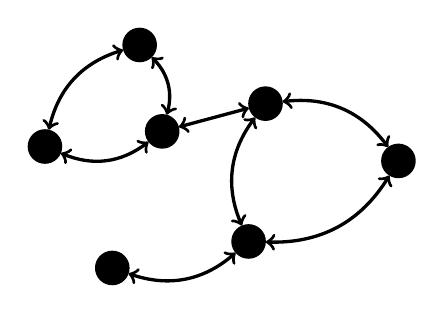
\begin{tikzpicture}[scale=0.75]
\GraphInit[vstyle=Simple]
\SetGraphUnit{2}
\tikzset{EdgeStyle/.style = {<->,very thick}}

\begin{scope}[rotate=-115]
  \Vertices{circle}{A,B,C,E,F}
\end{scope}
  \Vertex[x=4,y=0]{G}
  \Vertex[x=0,y=0.5]{D}
\Edges[style={bend right}](A,B,G,C,B)
\Edges[style={bend right}](D,E,F,D)
\Edges(D,C)
\end{tikzpicture}

\caption{Graph structure with multiple connected computational units:
  rich dynamics and powerful pattern recognition capabilities can
  result from the interaction of many simple nonlinear units.}
  \label{fig:graphStructure}
\end{figure}


\paragraph{Inductive learning (Learning from observations)} 
\begin{itemize}
	\item data driven, adaptive systems
	\item learning \& self-organization vs.\ deduction \& programming
	\item often seen as a plus: biologically inspired learning rules
\end{itemize}

\renewcommand{\descriptionlabel}[1]{\hspace{\labelsep}\emph{#1}}
\paragraph{Learning paradigms for ANNs}\mbox{}\\\\
Given: series of observations: $\vec{x}^{(1)}, \vec{x}^{(2)}, \ldots, \vec{x}^{(p)}$:
\begin{enumerate}[(1)]
\item {\bf Supervised Learning:} ''learning with a teacher''
  \begin{description}
  \item[Additional Information:] Additional training artefacts (``labels''): $y^{(1)}, y^{(2)}, \ldots, y^{(p)}$. Training is based on pairs $\{(\vec{x}^{(\alpha)},y^{(\alpha)})\}_{\alpha = 1, 2, ..., p}$
  \item[Goal:] Predict correct output for new (previously unseen) examples. 
  \item[Typical Problems:] classification and regression
  \end{description}
\item {\bf Unsupervised Learning:} ''self-organization''
  \begin{description}
    \item[Additional Information:] No additional information
    \item[Goal:] Detect statistical regularities, find a new representation of $\vec{x}$ useful for reasoning, decision making, prediction (e.g.\ efficient data storage)
      \item[Typical Problems:] clustering, categorization, source separation
  \end{description}
\item {\bf Reinforcement Learning:}
  \begin{description}
    \item[Additional Information:] additional ratings $r^{(1)}, r^{(2)}, \ldots, r^{(p)}$
    \item[Goal:] Selection of the right action $y$ for a given observation $\vec{x}$
    \item[Typical Problems:] learning association, strategy learning
  \end{description}
\end{enumerate}
\begin{figure}[h]
  \centering
\includegraphics[width=9cm]{section1_fig2}    
  \caption{Schematic illustration of reinforcement learning}
  \label{fig:reinforcementLearning}
\end{figure}

\vspace{5mm}

\textbf{Comments:}
\begin{itemize}
	\item (1)-(3) is a \emph{phenomenological} characterization of learning paradigms
	\item \underline{not} based on mathematical principles (e.g. same inductive 
		learning approaches for ''supervised'' and ''unsupervised'' 
		problems)
\end{itemize}

% -----------------------------------------------------------------------------

\subsection{Connectionist Neurons}

The components of an ANN are typically modeled as a simple
input-output function. In principle one could also use more complex components.

% -----------------------------------------------------------------------------
\subsubsection{Input-Output Relationship}
\textbf{Simple example:} Connectionist neurons can be modeled as a
\emph{linear filter} (see below) with a static non-linearity, i.e.\ as
a sequence of linear summation and a specific nonlinear function:
\vspace{5mm}

\begin{figure}[h]
  \centering
\begin{tabular}{c c c}
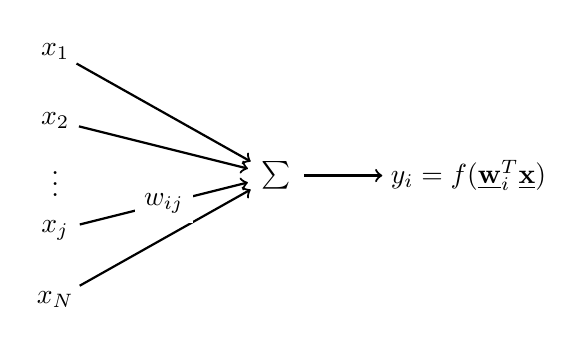
\begin{tikzpicture}[scale=0.7]
\GraphInit[vstyle=empty]
\SetGraphUnit{1}
\tikzset{EdgeStyle/.style = {->,thick}}
\SetVertexMath
\begin{scope}[rotate=-115]
\end{scope}
  \Vertex[x=4,y=0,L=\sum]{sumnode}
  \Vertex[x=0,y=2.25]{x_1}
  \Vertex[x=0,y=1]{x_2}
  \draw(0,0) node {\vdots};
  \Vertex[x=0,y=-1]{x_j}
  \Vertex[x=0,y=-2.25]{x_N}
  \Vertex[x=7.5,y=0,L={y_i=f(\vec{w}_i^T \vec{x})}]{y_i}
\Edge(x_1)(sumnode)
\Edge(x_2)(sumnode)
\Edge(x_N)(sumnode)
\Edge[label=$w_{ij}$](x_j)(sumnode)
\Edge(sumnode)(y_i)
\end{tikzpicture}
& \rule{2mm}{0pt}& \raisebox{18.5mm}{i.e.\ 
$y_i = f\Big(\underbrace{\sum_j \mathrm{w}_{ij} \mathrm{x}_j - \theta_i}_{h_i}\Big)$}
\end{tabular} 
\caption{Input-output function for the connectionist neuron.(\emph{cf.:} rate neurons, mean-field approximation, receptive field models \dots).}
  \label{fig:connectionistNeuron}
\end{figure}

\paragraph{Nomenclature:}
\[ \begin{array}{ll}
	\vec{x}: & \text{input vector with components } \mathrm{x}_j \\\\
	y_i: & \text{scalar output of neuron } i \\\\
	\vec{w}_i: & \text{weight vector of neuron } i \text{ with components }
		\mathrm{w}_{\underbrace{ij}_{out \leftarrow in}} \\\\
	\theta_i: & \text{threshold of neuron } i \\\\
	h_i: & \text{total input of neuron } i \\\\
	f: & \text{transfer function}
\end{array} \]
\\

\paragraph{Typical transfer functions:} In ANN applications the \emph{hyperbolic tangent}, \emph{logistic function} and in recent years the \emph{rectified linear unit} function are commonly used. Depending on interpretation (e.g.\ as probabilities when used at output units), one or the other might seem more intuitive. 
\begin{figure}[h]
  \centering
  \begin{tabular}[h]{c c}   
\parbox{4cm}{rectcified linear unit \\ $f_{(h)} = \max(0, h)$ } & 
\raisebox{-1cm}{\includegraphics[height=2cm]{section1_fig5a}}\\
\\
\parbox{4cm}{logistic function \\ $f_{(h)} = \frac{1}{1 + \exp (-\beta h)}$ } & 
\raisebox{-1cm}{\includegraphics[height=2cm]{section1_fig4}}\\
\\
\parbox{4cm}{hyperbolic tangent\\$f_{(h)} = \tanh(\beta h)$} &
\raisebox{-1cm}{\includegraphics[height=2cm]{section1_fig5}}
\end{tabular}
\end{figure}


\paragraph{Note:} The \emph{hyperbolic tangent}and the \emph{logistic function} transfer functions are computationally equivalent
\begin{equation}
	\begin{array}{ll}
	\frac{1}{1 + e^{-x}} 
	& = \frac{e^{\frac{x}{2}}}{e^{\frac{x}{2}} + e^{-\frac{x}{2}}} \\\\
	& = \frac{1}{2} \bigg\{
		\underbrace{\frac{e^{\frac{x}{2}} - e^{-\frac{x}{2}}}{
			e^{\frac{x}{2}} + e^{-\frac{x}{2}}}}_{
				\tanh \frac{x}{2}}
		+ \underbrace{\frac{e^{\frac{x}{2}} + e^{-\frac{x}{2}}}{
				e^{\frac{x}{2}} + e^{-\frac{x}{2}}}}_{1}
		\bigg\} \\\\
	& = \frac{1}{2} \big( \tanh \frac{x}{2} + 1 \big)
	\end{array}
\end{equation}
\begin{itemize}
	\itl scale input weights $\mathrm{w}_{ij}$ or slope parameter 
		$\beta$ by 2 (reparametrization)\\
	$\left.
	\begin{array}{l}
		\leadsto \text{shift output by -1} \\
		\leadsto \text{scale output by 2}
	\end{array}
	\right\} \text{change in units only} $
	\itR $\tanh x$
\end{itemize}

%\paragraph{Special transfer functions:} Special transfer function can be used depending up on the role of the output neuron in the network. For example, in case of linear feature extraction \emph{linear neurons} can be used. For classification application, \emph{binary} neuron can be used as the output neuron. \slideref{1.2 connectionist neurons}


\paragraph{Shortcut notation for neurons with thresholds:} The effect of a threshold $\theta_i$ can be accounted for by extending the input vector $\vec{x}$ by a constant entry $x_0=1$ with weight $w_{i0}$:\\

\begin{figure}[h]
  \centering
\begin{tabular}[h]{c c c}
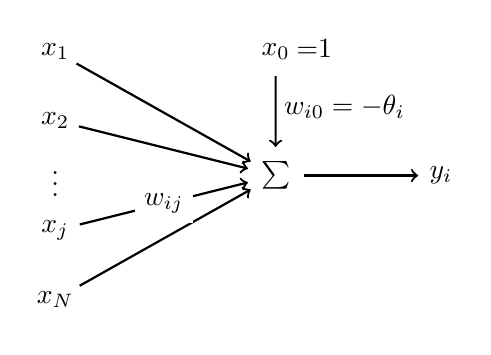
\begin{tikzpicture}[scale=0.7]
\GraphInit[vstyle=empty]
\SetGraphUnit{1}
\tikzset{EdgeStyle/.style = {->,thick}}
\SetVertexMath
\begin{scope}[rotate=-115]
\end{scope}
  \Vertex[x=4,y=0,L=\sum]{sumnode}
  \Vertex[x=0,y=2.25]{x_1}
  \Vertex[x=0,y=1]{x_2}
  \draw(0,0) node {\vdots};
  \Vertex[x=0,y=-1]{x_j}
  \Vertex[x=0,y=-2.25]{x_N}
  \Vertex[x=7,y=0]{y_i}
\Edge(x_1)(sumnode)
\Edge(x_2)(sumnode)
\Edge(x_N)(sumnode)
\Edge[label=$w_{ij}$](x_j)(sumnode)
\Edge(sumnode)(y_i)

\Vertex[x=4,y=2.25,L=x_0]{x_0}; \draw(4.7,2.3) node {=1}; 
\Edge(x_0)(sumnode)
\draw(5.25,1.25) node {$w_{i0}=-\theta_i$};
\end{tikzpicture}
&\rule{5mm}{0pt}& \raisebox{18.5mm}{
i.e. $y_i = f_{\big( \sum_j \mathrm{w}_{ij} \mathrm{x}_j \big)} = f_{( \vec{w}_i^T \vec{x} )}$
}
\end{tabular}
\caption{Shortcut notation for neurons with threshold}
\end{figure}
\vspace{5mm}

\noindent \textbf{Note:} With slight abuse of notation, in the following \\
\indent $\vec{w}$ will be used for $\rmat{ \mathrm{w}_1 \\ \vdots \\ \mathrm{w}_N}$ as well as for $\rmat{ \mathrm{w}_0 \\ \mathrm{w}_1 \\ \vdots \\ \mathrm{w}_N}$ \\\\
\indent $\vec{x}$ will be used for $\rmat{ \mathrm{x}_1 \\ \vdots \\ \mathrm{x}_N}$ as well as for $\rmat{ \mathrm{x}_0 \\ \mathrm{x}_1 \\ \vdots \\ \mathrm{x}_N}$

% -----------------------------------------------------------------------------

\subsubsection{Feature Detection and Evaluation}
\begin{itemize}
\item The weights $w_i$ can be interpreted as a ``linear filter''
\item Linear filters can be used for feature detection
  (cmp. ``receptive field'')
\end{itemize}
\textbf{Example:} Filters for points and edges:

\begin{figure}[h]
  \centering
\includegraphics[height=4cm]{section1_fig7}   
  \caption{Illustration: point and edge filters}
\end{figure}


\begin{equation}
	\underbrace{y_{kl}}_{
		\substack{\text{strength} \\ \text{of feature}}} 
		= \sum_{i,j = 0}^{m,n} 
			\underbrace{\mathrm{w}_{ij}}_{
				\substack{\text{filter} \\ \text{coefficients}}}
		\mathrm{x}_{\underbrace{(k+i)(l+j)}_{\text{pixel value}}}
\end{equation}

\begin{figure}[h]
  \centering
\includegraphics[width=8cm]{section1_fig8}  
  \caption{Linear coefficients for image filters}
\end{figure}


\begin{itemize}
\item $\vec{w}$ describing input summation in a sensory neuron is
often called its ''\emph{receptive field}''
\end{itemize}
\vspace{5mm}

\paragraph{Evaluation of filter output:} \label{sec:eval-filt-outp}
Assume a sample of data (black points) corresponding to size ($x_1$)
and weight ($x_2$) of apples and oranges (left plot, ``data
space''). Complex features are combinations $\vec{w}$ of such
elementary features and can be evaluated by projecting the datapoints
onto the weight vector ($\rightarrow$ right plot, ``feature space'').


\begin{figure}[h]
  \centering
\includegraphics[width=12.5cm]{section1_fig9}   
  \caption{Feature detection and evaluation}
\end{figure}


$\Rightarrow$ computing the match between feature and stimulus
(feature detection) and evaluating this match partitions the feature space into two half-spaces

% -----------------------------------------------------------------------------

\subsubsection{Special Transfer Functions}
\paragraph{Linear neuron}
\begin{equation} 
	f_{(h)} = \beta h
\end{equation}
$\Rightarrow$ extraction and detection of complex linear features
\paragraph{Binary neuron}
\begin{equation} 
	f_{(h)} = \mathrm{sign} (h)
\end{equation}
$\Rightarrow$ feature extraction and classification $\rightarrow$ perception
\begin{figure}[h]
  \centering
	\includegraphics[height=5.5cm]{section1_fig10}   
  \caption{The binary input-output function $y = f_{(h)} \in \{-1,+1\}$ 
partitions the feature space into two half-spaces.}
\end{figure}
\paragraph{Stochastic binary neuron}
In addition to the previous 2 deterministic transfer functions, stochastic
rules can be used to describe the response behavior of a
connectionist neurons (see \cite[ch.~39.1]{MacKay2003}), e.g.
\begin{equation}
	P_{(y \rightarrow -y)} = \frac{1}{1 + \exp (\beta y h)}
\end{equation}
$\beta$: noise parameter
\begin{figure}[h]
  \centering
\includegraphics[height=4.5cm]{section1_fig11}  
\caption{Stochastic binary neuron: The state of the stochastic binary neuron is not
deterministic, i.e.\ for a given input, its state can vary from trial
to trial.}
\end{figure}

% -----------------------------------------------------------------------------

\subsection{Multilayer Perceptron}

% -----------------------------------------------------------------------------

\subsubsection{Classes of Neural Networks}
The big variety of different ANNs can be classified according to their structure
 and the corresponding network graph
\[ \begin{array} {rcl}
\text{neural network} & \corresponds & \text{directed graph} \\
\text{(connectionist) neuron} & \corresponds & \text{node of the graph} \\
\text{connection between neurons} & \corresponds & \text{weighted edge} \\\\
\end{array} \]


\subsubsection*{Recurrent networks $\corresponds$ directed graphs containing cycles}
\begin{figure}[h]
  \centering
\includegraphics[height=2cm]{section1_fig12}   
  \caption{Recurrent neural networks are represented by graphs with cycles}
\end{figure}

\paragraph{Fields of application:}
\begin{itemize}
	\item models of dynamic systems
	\item spatio-temporal pattern analysis
	\item sequence processing
	\item associative memory and pattern completion
\end{itemize}
\paragraph{Examples:} Hopfield networks, Boltzmann machines,
\underline{i}nfinite \underline{i}mpulse \underline{r}esponse (IIR)
networks, \underline{l}ong \underline{s}hort-\underline{t}erm
\underline{m}emory networks (LSTM, \cite{HochreiterSchmidhuber1997})



\subsubsection*{Feedforward networks $\corresponds$ directed acyclic graphs}
\begin{figure}[h]
  \centering
\includegraphics[height=2cm]{section1_fig13}
  \caption{Feedforward neural networks are represented by graphs without cycles}
\end{figure}

\paragraph{Fields of application:}
\begin{itemize}
	\item association between variables
	\item prediction of attributes
\end{itemize}
\paragraph{Examples:} \underline{M}ulti\underline{l}ayer-\underline{P}erceptron (MLP), \underline{R}adial \underline{B}asis \underline{F}unction (RBF) network, \underline{S}upport \underline{V}ector \underline{M}achines (SVM) 

\paragraph{Prediction of attributes:} Many computational tasks involve the prediction of attributes. Depending on the type of predicted attribute, one distinguishes between \emph{regression} and \emph{classification}:
\\\\ 
\indent\textbf{Real-valued attributes:} $\rightarrow$ \emph{regression} problems
\begin{equation}
\begin{array}{lll}
	f: \mathbb{R}^N \rightarrow \mathbb{R} 
		& \text{ (or subsets)} 
		& \text{one target value} \\
	f: \mathbb{R}^N \rightarrow \mathbb{R}^M 
		& \text{ (or subsets)} 
		& \text{multivariate attributes}
              \end{array}
\end{equation}           
\\   
\indent \textbf{Ordinal attributes:} $\rightarrow$ \emph{classification} problems\\
              \indent let $S$ be the set of attributes $\{ a_1, a_2, \ldots, a_M \}$ 
              \[ f: \mathbb{R}^N \rightarrow S \]
              \indent \emph{special case:} two class problems, e.g. $f: \mathbb{R}^N \rightarrow \{-1, +1\}$\\\\
              \indent $\rightarrow$ predicting probabilities
              \\\\
              These approaches can be generalized for mappings from
              structured input to structured output

% -----------------------------------------------------------------------------

\subsubsection{The Multilayer-Perceptron for Regression}
\begin{figure}[h]
  \centering
\includegraphics[width=10cm]{section1_fig14} 
  \caption{Architecture of the MultiLayer Perceptron}
 \label{fig:MLP}
\end{figure}

\textbf{Simplifications used in this lecture:}
\begin{itemize}
	\item $\vec{x} \in \mathbb{R}^N, y_T \in \mathbb{R}$, i.e.\ scalar output, layered architecture
	\item training set: 
					$\big\{\vec x^{(\alpha)}, y_T^{(\alpha)} \big\}_{\alpha=1}^p$
	\item connections between subsequent layers only (except for bias node)
	\item similar transfer functions for all neurons
\end{itemize}
{\bf Nomenclature:}
\begin{equation*}
\begin{array}{ll}
	S_i^v & \text{activity of neuron } 
			\overbrace{(v, i)}^{\text{layer, unit}} := f(h_i^v) = f(\sum_j w_{ij}^{v,v-1} S_j^{v-1}-\theta_i^{v})\\\\
	S_0^0 = \mathrm{x}_0 = 1 & \text{activity of bias neuron} \\\\
	S_i^0 = \mathrm{x}_i & \text{input to MLP, } i^{\text{th}} 
			\text{ component} \\\\
	S_i^L = y_i & \text{output of MLP } (i=1 \text{ in figure } \ref{fig:MLP})\\\\
	\mathrm{w}_{ij}^{v'v} & \text{connection weight between neurons } 
			(v, j) \text{ and } (v', i) \\\\
	\mathrm{w}_{j0}^{v0} = \theta_j^v & \text{connection weight between 
			bias node and neuron } (v, j) \\\\
	h_i^v = \sum_j \mathrm{w}_{ij}^{vv-1} S_j^{v-1} & \text{total input
			of neuron } (v, i) \\\\
	f & \text{transfer function (sigmoid)}
\end{array}
\end{equation*}

\paragraph{MLP parameters}
\begin{itemize}
	\item[]
	$ \left.
	\begin{array}{l}
		\rightarrow \text{ number of layers} \\
		\rightarrow \text{ number of neurons per layer} 
	\end{array} 
	\right \} \text{''architecture''}$ 
	\itr $\left. \text{weights (including thresholds)} \right\} 
		\text{''model parameters''}$
	\itR \textbf{both} sets have to be chosen during \emph{model selection}! Examples on the MLP lecture slides page-13,14
\end{itemize} 
\paragraph{Visualization of weights and thresholds}

\begin{figure}[h]
  \centering
\includegraphics[height=3cm]{section1_fig15}  
  \caption{Visualisation of weights and thresholds}
\end{figure}

\textbf{Note:} Non-linear transfer functions are essential -- a 3
layered network of units with linear transfer functions is equivalent to a single connectionist neuron:
\begin{figure}[h]
  \centering
\includegraphics[height=3cm]{section1_fig16}  
  \caption{Importance of nonlinear transfer functions}
\end{figure}

\[ \begin{array}{rcl}
	y = \vec{w}^T \vec{z} = \vec{w}^T \vec{W} \vec{x} 
		= \widehat{\vec{W}} \vec{x} 
	& \corresponds & 
		\text{connectionist neuron}
\end{array} \]

\paragraph{MLPs are universal function approximators:} Even with
simple nonlinear functions, MLPs provide a model class with
powerful computational capabilities: For details, see e.g.\
\textcite{Funahashi1989} and \textcite{HornikEtAl1989}.
\\\\
\textbf{Theorem:} Let $y_{(\vec{x})}^*$ be a continuous, real valued function over a
compact interval $K$. Let
\[ \hat{y}_{(\vec{x})} = \sum_{i=1}^M \mathrm{w}_i^{21} 
	f_{\Big( \sum\limits_{j=1}^N \mathrm{w}_{ij}^{10} 
		\mathrm{x}_j - \theta_i \Big)}
\]
be a three-layered MLP with a non-constant, bounded, monotonously increasing and continuous function $f: \mathbb{R} \rightarrow \mathbb{R}$.
\\\\
Then there exists a set of parameters $M, N \in \mathbb{N}$ and $\mathrm{w}_i^{21}, \mathrm{w}_{ij}^{10}, \theta_i \in \mathbb{R}$ such that for every $\varepsilon > 0$:
\[ \max_{\vec{x} \in K} \Big| \hat{y}_{(\vec{x})} - y_{(\vec{x})}^* \Big| 
	\leq \varepsilon
\]

% -----------------------------------------------------------------------------

\subsubsection{Performance Measures and Model
  Selection} \label{sec:perf-meas-model} \textbf{Remark:} For both
regression and classification problems, the goal is to find a model
that predicts the observed outputs (and potential future observations)
as good as possible. This goodness of fit can be quantified via
\emph{error} or \emph{cost functions}. Below, we describe error
functions for \emph{regression} problems, for classification problems,
see \ref{sec:class-problems}.


\paragraph{Prediction of attributes}
\[ \underbrace{\vec{x} \in \overbrace{\mathbb{R}^N}^{
	\substack{\text{data} \\ \text{point}}}
	}_{\substack{\text{feature} \\ \text{vector}}}
   \longrightarrow 
   \underbrace{y \in \overbrace{\mathbb{R}}^{\text{label}}
	}_{\text{attribute}}
\]
\[ \begin{array}{ll}
	y_T: & \text{true value of attribute} \\
	y_{(\vec{x})}: & \text{predicted value of attribute (e.g. by MLP)}
\end{array} \]

\paragraph{Error measure (individual cost / individual loss):}
The error measure quantifies the cost of a wrong prediction (e.g.\ loss in \$\$, $\ldots$) and determines the ``goodness'' of a solution.
\\\\
\textbf{Example error functions}
\begin{figure}[h]
  \centering
\includegraphics[width=14cm]{section1_fig17}   
  \caption{Example error functions: choice depends on task setting \& assumptions regarding noise.}
\end{figure}

\begin{itemize}
	\item several choices possible $\Rightarrow$ one must be made
	\item predictor will depend on error measure!
\end{itemize}
Most common error measure: 
\begin{equation} \tag{quadratic error}
	e_{(y_T, \vec{x})} = \frac{1}{2} \big( y_T - y_{(\vec{x})} \big)^2
\end{equation}
\vspace{2mm}

\paragraph{Performance measure:}
How many \$\$ per prediction do I have to spend on average?\\
\indent $\Rightarrow$ mathematical expectation
\begin{equation} \tag{generalization error}
	E^G = \underbrace{<e>_{y_T, \vec{x}}}_{ 
		\substack{\text{mathematical} \\ \text{expectation} \\
			\text{w.r.t } y_T \text{ and } \vec{x}}}
	= \int \int d \vec{x} d y_T P_{(y_T, \vec{x})} e_{(y_T, \vec{x})}
\end{equation}
$P_{(y_T, \vec{x})}$: joint \underline{p}robability \underline{d}ensity \underline{f}unction (pdf) of observations
\[ \left. \begin{array}{ll}
	\text{good predictor:} & \text{low value for } E^G \\
	\text{bad predictor:} & \text{high value for } E^G
\end{array} \right \} E^G \eqexcl \min \]
\underline{but:}
\begin{itemize}
\item $P_{(y_T, \vec{x})}$ is - in general - not known.
\item If we knew it, there would be no need for learning!
\itr $E^G$ cannot be minimized directly.
\end{itemize}

\paragraph{Inductive learning through \underline{e}mpirical \underline{r}isk \underline{m}inimization (ERM)}\mbox{}\\\\
\textbf{General idea}
\begin{center}
mathematical expectation $\rightarrow$ empirical average over a ''training set''
\end{center}

\emph{training set of observations:} $\left\{ \Big(\vec{x}^{(\alpha)}, y_T^{(\alpha)} \Big) \right\}, \alpha = 1, \ldots, p$
\begin{equation} \tag{training error, empirical risk $E^T$}
	E^T = \frac{1}{p} \sum_{\alpha = 1}^p e^{(\alpha)}
\end{equation}
\textbf{Model selection:} Find model (parameters) such that: $E^T \eqexcl \min$
\\\\
{\bf Consequences}
\begin{itemize}
\item \emph{Validation:} Is the selected model indeed a good predictor?
\item \emph{Mathematical analysis:} When does ''$E^T \eqexcl \min$'' imply ''$E^G$ is small (enough)''? $\Rightarrow$ statistical learning theory, ch. \ref{sec:learn-theory-supp}. 

\end{itemize}


\begin{figure}[h]
  \centering
 \includegraphics[height=5cm]{section1_fig18}   
  \caption{model selection and overfitting}
\end{figure}

% -----------------------------------------------------------------------------

\subsubsection{Optimization of Model Parameters: Gradient Descent}
  \begin{center}
  \begin{tabular}{c c c}
architecture & vs. & model parameters\\
{\footnotesize (number of layers and nodes)} & & {\footnotesize(weights, thresholds)}    
  \end{tabular}
  \end{center}
Learning can affect both aspects; here we focus on learning the model parameters.\\\\
\emph{training set:} $\Big\{ \Big (\vec{x}^{(\alpha)}, y_T^{(\alpha)} \Big) \Big\}, \alpha = 1, \ldots, p$
\\\\
\emph{training error} $E^T$ for the given training set: $E_{[\vec{w}]}^T = \frac{1}{p} \sum\limits_{\alpha = 1}^p e_{[\vec{w}]}^{(\alpha)}$

\paragraph{Gradient Descent}
\begin{figure}[h]
  \centering
\includegraphics[width=\textwidth]{section1_fig19}  
  \caption{illustration of gradient descent}
\end{figure}

\begin{equation}
	\begin{array}{ll}
	\Delta \mathrm{w}_{ij}^{v'v} 
	& = \underbrace{-\hat{\eta}}_{ \substack{\text{learning} \\ 
			\text{step} } }
		\underbrace{\frac{\partial E_{[\vec{w}]}^T}{
			\partial \mathrm{w}_{ij}^{v'v}}}_{
				\substack{
					\text{gradient vector:} \\ 
					\text{direction of} \\
					\text{steepest ascent} } } \\\\
	& = \underbrace{-\eta}_{\eqexcl \frac{\hat{\eta}}{p}}
		\sum\limits_{\alpha = 1}^p \frac{\partial e_{[\vec{w}]}^{(\alpha)}}{
			\partial \mathrm{w}_{ij}^{v'v}}
	\end{array}
\end{equation}
\paragraph{Calculation of the gradient:}
\begin{equation} \label{eq:gradientMLP}
	\frac{\partial e_{[\vec{w}]}^{(\alpha)}}{\partial \mathrm{w}_{ij}^{v'v}}
	= \underbrace{ \frac{\partial e_{[\vec{w}]}^{(\alpha)}}{\partial 
		y_{(\vec{x}^{(\alpha)}, \vec{w})}} }_{
			\substack{\text{factor depending} \\
				\text{on cost function}}}
	  \cdot \underbrace{\frac{\partial y_{(\vec{x}^{(\alpha)}, \vec{w})}}{
		\partial \mathrm{w}_{ij}^{v'v}} }_{ 
			\substack{\text{factor depending on} \\
				\text{model class (e.g. MLP)}}}
\end{equation}
for the quadratic error we obtain: 
\begin{equation}
	\frac{\partial e_{[\vec{w}]}^{(\alpha)}}{
		\partial y_{(\vec{x}^{(\alpha)}, \vec{w})} } \quad
	=\frac{\partial}{\partial y_{(\vec{x}^{(\alpha)}, \vec{w})} }
	\frac{1}{2} (y_{(\vec{x}^{(\alpha)}, \vec{w})} - y_T)^2 \quad
	= y_{(\vec{x}^{(\alpha)}, \vec{w})} - y_T
\end{equation}
\paragraph{Problems of the gradient descent method}
\begin{itemize}
	\item convergence to local minima\\
              (problem of all gradient-based, local optimization methods)
	\item choice of $\eta$ may be critical (slow convergence vs. 	
		oscillations)
\end{itemize}

% -----------------------------------------------------------------------------

\subsubsection{The Backpropagation Method}
Backpropagation of errors is a computationally efficient method for calculating the  derivatives
\begin{equation}
	\frac{\partial y_{(\vec{x}^{(\alpha)}, \vec{w})}}{
		\partial \mathrm{w}_{ij}^{v'v}}
\end{equation}
required to determine the parameters of Multilayer-Perceptrons (MLPs) via gradient descent (see eq.~\ref{eq:gradientMLP}).
\begin{itemize}
	\itR can be extended to other feedforward networks
	\itR efficient way to do message passing in directed acyclic graphs
\end{itemize}
\begin{figure}[h]
  \centering
\includegraphics[height=3.5cm]{section1_fig20}   
  \caption{schema backpropagation}
\end{figure}
Smart application of the chain rule exploiting $h_i = \vec{w}_i^T\vec{s}-\theta_i$:
\begin{equation}
	\frac{\partial y}{\partial \mathrm{w}_{ij}^{v'v}}
		= \underbrace{\frac{\partial y}{\partial h_i^{v'}}}_{ 
			\substack{\coloneqq \delta_i^{v'} \\
				\text{''local error''} \\
				\text{at neuron} \\
				(v', i)}}
		  \cdot 
		  \underbrace{\frac{\partial h_i^{v'}}{\partial 
		  	\mathrm{w}_{ij}^{v'v}}}_{
				\substack{= S_j^v \\
				\text{activity} \\
				\text{of neuron} \\
				(v, j)}}
\end{equation}
\emph{Note:} this definition $\delta_i^{v'}:= \partial y/\partial
h_i^{v'}$ of a units local effect on $y$ is slightly different from
the definition $\delta_i^{v'}:= \partial e / \partial h_i^{v'}$ of ``local error'' given in e.g.\ \textcite{Bishop2006}. 


\paragraph{Forward propagation step:}  calculation of \emph{activities}
\begin{align} \tag{initialization: inputs}
	S_j^0 & = \mathrm{x}_j^{(\alpha)} \\
\tag{propagation}
	S_j^v &= f_{\Big( \sum\limits_{(\gamma, h) \in \text{ parents } (v, j)}
			\mathrm{w}_{jh}^{v\gamma} S_h^{\gamma} \Big) }
\end{align}

\paragraph{Backpropagation step:} calculation of \emph{''local errors''}
\begin{align} \tag{initialization: outputs}
  \delta_1^v &= f'_{(h_1^v)}\\
  \delta_i^{v'} 
  & = \sum\limits_{(\beta, l) \in \text{ children } (v', i)}
  \frac{\partial y}{\partial h_l^{\beta}} \cdot
  \frac{\partial h_l^{\beta}}{\partial h_i^{v'}} \\
  & = \sum\limits_{(\beta, l) \in \text{ children } (v', i)}
  \delta_l^{\beta} \mathrm{w}_{li}^{\beta v'} f'_{(h_i^{v'})}\\
\tag{propagation}
	 &= f'_{(h_i^{v'})} \sum_{(\beta, l) 
			\in \text{ children } (v', i)}
		\delta_l^{\beta} \mathrm{w}_{li}^{\beta v'}
\end{align} 

Computational complexity: $\mathcal{O}(n)$, $n$: number of weights \& thresholds

% -----------------------------------------------------------------------------

\subsubsection{Summary of the Gradient Descent Method}
{\bf Initialization:} random numbers, such that $h_i^v$ approx. $\mathcal{O}(1)???$
\begin{itemize}
	\item numbers too large: transfer function saturates\\
          $\leadsto$ gradients become too small
	\item numbers too small: neurons operate in the linear regime of $f$\\
          $\leadsto$ MLP becomes equivalent to one connectionist neuron
\end{itemize}
{\bf Stopping criterion}
\begin{itemize}
	\item fixed number of iterations
	\item fixed CPU-time
	\item $E^T$ falls below a predefined value
	\item $\frac{\Delta E^T}{E^T}$ falls below a predefined value
	\item validation criterion fulfilled
\end{itemize}

% -----------------------------------------------------------------------------

\subsubsection{Validation of Model Selection Results}
Assessment of prediction quality $\Rightarrow$ estimation of $E^G$
\paragraph{Test Set Method:} \mbox{}
\begin{equation*}
  \text{observations} \left \{ 
   \begin{array}{l}
   	\text{training data } \Big\{ \Big( \vec{x}^{(\alpha)}, y_T^{(\alpha)}
		\Big) \Big\}, \alpha = 1, \ldots, p \\
	\rightarrow \text{for selection of model parameters} \\\\
	\text{test data } \Big\{ \Big( \vec{x}^{(\beta)}, y_T^{(\beta)}
		\Big) \Big\}, \beta = 1, \ldots, q \\
	\rightarrow \text{for estimation of the generalization error}
\end{array} \right.
\end{equation*}

\begin{figure}[h]
  \centering
\includegraphics[height=6cm]{section1_fig21}  
  \caption{symptoms of overfitting: training vs.\ generalization error}
\end{figure}


\textbf{Notes:} 
\begin{itemize}
\item Test data must not be used for selection of model parameters.\\
Therefore, the method is problematic if only few data available
\item Estimate for the generalization performance of a \emph{specific} model. 
\end{itemize}

\paragraph{Resampling methods: N-Fold Cross-Validation}
\begin{enumerate}[(1)]
\item The set of all observations $D$ is partitioned into $n$ disjunct subsets $D_j$ such that $\bigcup\limits_{j = 1}^n D_j = D$\\
  \begin{figure}[h]
    \centering
\includegraphics[height=5cm]{section1_fig22}    
    \caption{Crossvalidation}
    \label{fig:crossvalidation}
  \end{figure}

\item On each of the training datasets $D$ / $D_j$, train a network $N_j$ and compute average prediction error $\hat{E}_i^G$ on the test set $D_j$.
\end{enumerate}

\textbf{Estimation of $E^G$:}
\begin{equation}
	\widehat{E}^G = \quad\frac{1}{N} \sum_{i=1}^N \hat{E}_i^G= \quad\frac{1}{p} \sum_j \sum_{\alpha \in D_j} e^{(\alpha)}
\end{equation}
\begin{itemize}
\item Typical choice: n $\approx$ 5 \dots 10
\item ``leave-one-out cross-validation'': $n = p$ 
\end{itemize}
\emph{Variance of the cross-validation estimator}
\begin{equation}
	\mathrm{var} \Big( \widehat{E}^G \Big) = \frac{n-1}{n}
		\sum_{j = 1}^n \Big( \underbrace{\widehat{E}_j^G}_{
				\substack{\text{test error} \\
					\text{on } D_j}}
			- \widehat{E}^G \Big)^2
\end{equation}
\textbf{Notes:} 
\begin{itemize}
\item n-fold cross-validation is only used for estimating $E^G$
\item the resampling procedure yields $n$ different sets of parameters
\item for selecting the final model parameters \underline{all data} are used!
\item estimates average prediction performance of the \emph{combination} (
  architecture + training method) ($\leftrightarrow$ test-set-method)
\end{itemize}
% -----------------------------------------------------------------------------

\newpage					% NEWPAGE for visual reasons
\subsection{Additional Topics}

% -----------------------------------------------------------------------------

\subsubsection{Stochastic Approximation and On-line Learning}
Gradient descent (MLP example):
\begin{equation}
	\begin{array}{ll}
	\Delta \mathrm{w}_{ij}^{v'v} 
	& = -p \eta \frac{\partial E_{[\vec{w}]}^T}{
		\partial \mathrm{w}_{ij}^{v'v}} \\\\
	& = -\eta \sum\limits_{\alpha = 1}^p \frac{
		\partial e_{[\vec{w}]}^{(\alpha)}}{
		\partial \mathrm{w}_{ij}^{v'v}} \\\\
	\end{array}
\end{equation}
{\bf Batch learning:} All observations are used for every weight update.
\\\\
{\bf On-line learning:} Sequential processing of observations
\begin{itemize}
\item  one weight update per data point (''learning while doing'')
  \itl learning and adaption in \emph{non-stationary} environments
\end{itemize}
Online learning for MLPs can easily be implemented:
\begin{algorithm}
  \DontPrintSemicolon
  $t \leftarrow 1$\;
  \Begin{
    $\eta_{t} \leftarrow \frac{\eta_0}{t}$ 
    \hfill (learning schedule, depends on learning goal) \;
    select next data point: $\left( \vec{x}^{(\alpha)}, y_T^{(\alpha)} \right)$\;
    change weights:$\big( \Delta \mathrm{w}_{ij}^{v'v} \big)^{t+1} = -\eta_t 
    \frac{\partial e_{[\vec{w}^{(t)}]}^{(\alpha)}}{
      \partial \mathrm{w}_{ij}^{v'v}}$\;
    $t \leftarrow t + 1$}
\caption{On-line learning of MLP-weights}
\end{algorithm}
\newline
In practice, online learning has proven to be \emph{robust}: 
\begin{itemize}
	\item convergence to (good) minima of $E^T$
	\item less affected by the ''local optimum'' problem (stochastic update)
\end{itemize}
\emph{But:} no general proof of convergence yet
\begin{enumerate}[(1)]
\item Theorem by Robbins \& Monro (1951): ''stochastic approximation''\\
  Holds only for convex optimization problems.\slideref{For theorem
    statement, see lecture slides}\footnote{For proof, see
    supplementary material}
\item Theorem by Bottou (1998): Almost sure convergence only to extrema of $E^T$
(not necessarily minima)\\
  $\Rightarrow$ conditions not necessarily fulfilled for MLPs with
  sigmoid transfer functions.\slideref{For theorem
    statement, see lecture slides}\footnote{For proof, see supplementary material}
\end{enumerate}
% -----------------------------------------------------------------------------

\subsubsection{Improved Gradient Descent Optimization}
\begin{enumerate}[(a)]
\item \textbf{Impulse terms / Momentum}
  \begin{center} \includegraphics[height=4cm]{section1_fig23} \end{center}
  Oscillations can be reduced by introducting ``momentum'' or impulse terms into the weight-update 
  \begin{equation}
    \Delta \vec{w}_{t + 1} = -\hat{\eta} \frac{\partial E^T}{
      \partial \vec{w}}\bigg|_{\vec{w}_t} + 
    \underbrace{\mu \Delta \vec{w}_t}_{
      \substack{\text{impulse} \\
        \text{term}}}
  \end{equation}
  \begin{center} \includegraphics[height=4cm]{section1_fig24} \end{center}
  Impulse terms can be interpreted as smoothing the weight updates
  with an exponentially weighted running average.
\item \textbf{Adaptive step size}
  \begin{center} \includegraphics[height=4cm]{section1_fig25} \end{center}
  \[ \eta_{t + 1} = \left \{ 
    \begin{array}{lll}
      \rho \, \eta_t, 
      & \text{if } \Delta E^T < 0,
      & \text{increase step size, if } E^T \downarrow \\\\
      \delta \, \eta_t, 
      & \text{if } \Delta E^T > 0,
      & \text{decrease step size, if } E^T \uparrow 
    \end{array} \right.
  \]
  typical values: $\rho = 1.1, \delta = 0.5$
\end{enumerate}
% -----------------------------------------------------------------------------

\subsubsection{The Conjugate Gradient Method}
\[ \text{local optimization} \left \{
	\begin{array}{l}
		\text{choice of direction} \Rightarrow 
			\text{conjugate direction} \\\\
		\text{choice of step size} \Rightarrow
			\text{line search method}
	\end{array} \right.
\]
{\it for details \& implementation see Numerical Recipes, 2nd edition chapter 10.2 \& 10.6}

\paragraph{Line search method}\mbox{}\\
Search for the minimum of the cost \emph{along a given direction} in
parameter space.
\begin{figure}[h]
  \centering
   \includegraphics[height=5cm]{section1_fig26}   
  \caption{linesearch}
  \label{fig:linesearch}
\end{figure}
There are different alternatives to find this minimum, one of them is
\emph{parabolic interpolation}:
\begin{algorithm}
   \DontPrintSemicolon
  \textbf{Initialization:} $a_0, b_0, c_0 (\text{on } \lambda \vec{d}_t); E_{(a_0)}^T, E_{(b_0)}^T > E_{(c_0)}^T$\;
  \While{stopping criterion not fulfilled}{
			\vspace{2mm}
			Fit a parabola through the three points $a_t, b_t, c_t$ \\[2mm]
			Calculate location $d_t$ of its minimum\\[0mm]
			Set $c_{t+1} = d_t,\quad b_{t+1} = c_t,\quad a_{t+1} = \left \{ 
			  \begin{array}{ll}
			 		a_t, & E_{(a_t)}^T < E_{(b_t)}^T \\
			 		b_t, & \text{else}
			 	\end{array} \right.$ 
		}
    \caption{parabolic interpolation. Note: the last step effectively
      selects the best 3 points for the next iteration. Problem: works
      only if close enough to local minimum.}
\end{algorithm}

\paragraph{The conjugate direction}\mbox{}\\
\emph{Problem with standard gradient direction:} Minimum $\vec{w}_t$
after line search: new gradient $\perp$ old direction $\leadsto$
oscillations. \slideref{Oscillations}

\paragraph{Definition of conjugate direction $\vec{d}_{t+1}:$}\mbox{}\\
The component of the gradient parallel to the old direction ($\vec{d}_t$) 
should remain zero along the new direction 
($\vec{d}_{t+1}$). \slideref{Conjugate\\Direction} It can be computed as:
\begin{equation} \tag{gradient}
	\vec{g}_{t+1} \coloneqq \frac{\partial E^T}{\partial \vec{w}}
		\bigg|_{\vec{w}_{t+1}}
\end{equation}
\begin{equation} 
	\vec{d}_{t+1} = -\vec{g}_{t+1} + \beta_t \vec{d}_t
\end{equation}
\begin{equation}
	\beta_t = \underbrace{ \frac{\vec{g}_{t+1}^T 
		\big( \vec{g}_{t+1} - \vec{g}_t \big)}{
		\vec{g}_t^T \vec{g}_t} }_{
			\text{Pollach-Ribiere rule}}
\end{equation}
The conjugate gradient method therefore contains the following steps
\begin{algorithm}
  \DontPrintSemicolon
  \textbf{Initialization:} $\vec{w},\quad \vec{d} = - \vec{g}$ \;
  \While{stopping criterion not fulfilled}{
			\vspace{1mm}
			Minimize $E^T$ along $\vec{d}$ using line-search 
				\quad $\rightarrow$ new $\vec{w}$ \\[1mm]
			Calculate the new conjugate direction 
				\quad $\;\,\rightarrow$ new $\vec{d}$
			\vspace{1mm}
		}
  \caption{Conjugate gradient method}
\end{algorithm}


\paragraph{Remark:} Conjugate Gradient realizes efficient gradient
descent with adaptive step size and impulse term
\begin{itemize}
\item step size: calculated via line search
\item impulse parameter: given by $\beta_t$
\end{itemize}
$\Rightarrow$ preferred gradient-based method for unconstrained optimization
% -----------------------------------------------------------------------------

\subsubsection{Overfitting and Underfitting}
\textbf{Typical task:} Given a limited set of data $(x_T,y_T)$, find a model to describe the relation between x and y and make predictions $y^*(x_N)$ for new data $x_N$. 
\[ \begin{array}{ll}
	\includegraphics[height=5cm]{section1_fig27}
	& y_T = y_{(\vec{x})}^* + \underbrace{\eta}_{\text{noise}}
\end{array} \]

\noindent {\bf Three cases:}
\begin{enumerate}[I.]
\item {\bf Model is too simple} (e.g. MLP is too small)\\
\indent $\leadsto y^*$ cannot be approximated well
\[ \begin{array}{ll}
	\includegraphics[height=4cm]{section1_fig28}
	& \left. \begin{array}{l}
		E^T \text{ large} \\
		E^G \text{ large}
	\end{array} \right \} E^T \text{ approx. } E^G \\\\
	& \text{''underfitting''}
\end{array} \]
\item{\bf Model complexity matches} (e.g. MLP has the right size)
\[ \begin{array}{ll}
	\includegraphics[height=4cm]{section1_fig29}
	& \left. \begin{array}{l}
		E^T \text{ small} \\
		E^G \text{ small}
	\end{array} \right \} E^T \text{ approx. } E^G \\\\
\end{array} \]
\item {\bf Model is overly complex} (e.g. MLP is too large)
\[ \begin{array}{ll}
	\includegraphics[height=4cm]{section1_fig30}
	& \left. \begin{array}{l}
		E^T \text{ small} \\
		E^G \text{ large}
	\end{array} \right \} E^T \ll E^G \\\\
	& \text{''overfitting''}
\end{array} \]
\begin{itemize}
	\itR often happens if $E^T$ does not vary strongly over a large volume 
		of parameter space
	\itR using a different sample of observations (from the same underlying 
		distribution) may lead to a large shift of the minimum of $E^T$ 
		in parameter space.\slideref{Overfitting}
\end{itemize}
\end{enumerate}
% -----------------------------------------------------------------------------

\subsubsection{Bias and Variance}
Complexity of a model class influences how well it can describe
different data sets but also how much parameter estimates are affected
by random fluctuations in the training data. The bias and variance of
an estimator quantify these two statistical aspects and together
determine its generalization performance.\footnote{The total
  generalization error can always be separated into the three terms
  squared bias, variance, and the error variance.}

\paragraph{Example scenario:} Data $y_T = \underbrace{y_{(\vec{x})}^*}_{\substack{\text{true} \\ \text{relationship}}} + \underbrace{\eta}_{\text{noise}}, \indent\vec{x} \in \mathbb{R}^N, y_T \in \mathbb{R}$
\[ \begin{array}{ll}
	\eta: & \text{zero mean additive noise} \\
	P_{(\vec{x})}: & \text{pdf of data points} \\
	P_{(y|\vec{x})}: & \text{conditional pdf of attributes}
\end{array} \]
\emph{Assessing generalization performance:}
\begin{enumerate}
\item sample many iid.\ datasets of equal length from $ P_{(y_T,
    \vec{x})} = P_{(y_T| \vec{x})} P_{(\vec{x})}$
\item fit one MLP to every dataset using squared error as individual
  cost.
\end{enumerate}
\textbf{Remark:} $\vec{x}, y_T$ are random variables
\begin{itemize}
	\itr $\vec{w}$ (model parameters) are random variables
	\itr $y_{(\vec{x};\vec{w})}$ (predicted values) are random variables
\end{itemize}
Generalization performance is based on the mathematical expectation
\begin{equation} \tag{''ensemble average''}
	\Big< \Big( \underbrace{y_{(\vec{x};\vec{w})}}_{y} 
		- \underbrace{y_{(\vec{x})}^*}_{y^*} 
		\Big)^2 \Big>_{
		\text{all datasets}}
\end{equation}
With
\begin{equation}
	\begin{array}{ll}
	(y - y^*)^2 
	& = (y - <y> + <y> - y^*)^2 \\
	& = (y - <y>)^2 + (<y> - y^*)^2 + 2 \underbrace{(y - <y>)}_{
		\substack{ = 0 \\ \text{when averaged}}} 
		(<y> - y^*)
	\end{array}
\end{equation}
one obtains the following decomposition of the generalization error
into bias and variance:
\begin{equation}
	\big< (y - y^*)^2 \big> = 
		\underbrace{(<y> - y^*)^2}_{\text{bias}^2}
		+ \underbrace{\big< (y - <y>)^2 \big>}_{\text{variance}}
\end{equation}
\begin{itemize}
\item useful for scenarios, where a deviation measure makes sense
\item not useful however for classification problems (other
  ansatz needed)
\end{itemize}

\begin{figure}[h]
  \centering
  \includegraphics[height=5cm]{section1_fig31}  
  \caption{Illustration of the bias-variance decomposition: different
    datasets result in different estimates ($y=y_{(\vec{x};\vec{w})}$,
    dashed lines). The bias is given by the mean squared deviation
    between their average ($\langle y \rangle$, thick line) and the
    true values ($y^*$, thin line). The variance quantifies the
    variability of the individual sample-based estimates $y$ around
    their mean $\langle y \rangle$.}
  \label{fig:bias-variance}
\end{figure}

\paragraph{Bias-variance trade-off:} While \emph{variance} describes
the amount by which our estimate is expected to vary if we compute it
using a different training dataset, its \emph{bias} describes the
systematic error due to our approximation with a (too) simple
(e.g. linear) model. As a result, more flexible (complex) statistical
methods typically have lower bias but higher variance. This
bias-variance trade-off applies to many inductive learning problems.
\begin{figure}[h]
    \centering
    \includegraphics[height=7.5cm]{section1_fig32}    
    \caption{Illustration of the bias-variance trade-off. Underfitting
      typically occurs when bias dominates the total deviation
      (too simple models), overfitting when variance dominates (too
      complex models).}
    \label{fig:bias-variance-tradeoff}
  \end{figure}
\paragraph{Examples for model classes of different complexity}
\begin{itemize}
	\itr MLP with increasing number of layers/units
	\itr polynomials of increasing degree\slideref{Duda\&Hart\\ p.467}
\end{itemize}

\paragraph{Relation to generalization performance} (for above example scenario)
\begin{equation}
	E^G = \big< e^G \big>_{P_{(\vec{x})}}, \text{ where } 
		e^G = \big< (y_{(\vec{x};\vec{w})} - y_T)^2 \big>_{
			P_{(y_T|\vec{x})}}
\end{equation}
\begin{equation}
	\begin{array}{ll}
	e^G
	& = \big< (y - y_T)^2 \big> \\\\
	& = \big< (y - y^* + y^* - y_T)^2 \big> \\\\
	& = (y - y^*)^2 + \big< (y^* - y_T)^2 \big> + 2(y - y^*) 
		\underbrace{ \big< (y^* - y_T) \big> }_{= 0} \\
	& = (y - y^*)^2 + \sigma_{\eta}^2
	\end{array}
\end{equation}
\begin{equation}
	\big< e^G \big>_{\text{ensemble}} 
	= \big< \underbrace{(y - y^*)^2}_{\text{bias}^2 + \text{variance}}
		\big>_{ \text{ensemble}} + \sigma_{\eta}^2
\end{equation}
\begin{itemize}
\item for classification example, see {\it cf. slide: Duda \& Hart 470}
\item relationship bias-variance usually not additive and can be
  non-linear
\end{itemize}
% -----------------------------------------------------------------------------


\subsubsection{Regularization}
Complex model but few observations $\rightarrow$ danger of overfitting
\begin{itemize}
\itr include additional (prior) knowledge about the problem
\itr bias the selection procedure towards a certain model class
\end{itemize}
\begin{equation} \tag{risk function}
	R_{[\vec{w}]} = \underbrace{ E_{[\vec{w}]}^T }_{
			\substack{\text{training} \\ \text{error}}}
		+ \underbrace{ \lambda E_{[\vec{w}]}^R }_{
			\substack{\text{regularization} \\ \text{term}}}
		\eqexcl \min 
\end{equation}
\[ \begin{array}{ll}
	E^R: & \text{penalizes certain models} \leadsto \text{''soft'' 
		restrictions on model space} \\
		& \text{(using prior knowledge of solution)}\\
	\lambda: & \text{regularization parameter; trade-off between 
		observations and prior knowledge}
\end{array} \]
\paragraph{Example I: inclusion unspecific knowledge:} weight decay
\begin{equation}
	E_{[\vec{w}]}^R = \frac{1}{2} \sum_{i, j, v', v} 
		\big( \mathrm{w}_{ij}^{vv'} \big)^2
\end{equation}
\begin{itemize}
  \itr penalty for models with many weights of large absolute value
  \itr implicit smoothness assumption (e.g.\ MLPs smaller weights
  $\sim$ smoother input-output functions)
\end{itemize}
\emph{Minimization of the risk R through gradient descent:}
\begin{equation}
	\Delta \mathrm{w}_{ij}^{vv'} \sim 
		-\frac{\partial R}{\partial \mathrm{w}_{ij}^{vv'}}
= -\left(\frac{\partial E^T}{\partial \mathrm{w}_{ij}^{vv'}}
  +\frac{\partial E^R}{\partial \mathrm{w}_{ij}^{vv'}}\right) 
= -\underbrace{\frac{\partial E^T}{\partial \mathrm{w}_{ij}^{vv'}}}_{
		\substack{\text{e.g. via} \\ \text{backprop}}}
	- \underbrace{\lambda \mathrm{w}_{ij}^{vv'}}_{
		\substack{\text{decay} \\ \text{term}}}
\end{equation}
\begin{itemize}
  \itl Parameters which are not supported by data (can be estimated
  less reliably) decay to zero.
  \itl Different components of the weight vector can be estimated more or less reliably from the data. They are affected differently by weight decay and therefore differ more or less from the unregularized estimate $\vec{w}^*$ minimizing training Error $E^T$
\end{itemize}

\begin{figure}[h]
  \centering
\includegraphics[height=5cm]{section1_fig33}  
  \caption{weight decay}
  \label{fig:weight-shrinkage}
\end{figure}


\begin{tabular}{l l l }
$\mathrm{w}_1$: & "badly" supported parameter& $\rightarrow$ shrinks more\\
$\mathrm{w}_2$: & "well" supported parameter & $\rightarrow$ shrinks less
\end{tabular}
\paragraph{Example II: inclusion of specific knowledge:} symmetries
\begin{enumerate}[(a)]
\item Odd vs. even function
\begin{equation}
	E_{[\mathrm{w}]}^R = \frac{1}{2p} \sum_{\alpha = 1}^p 
		\Big( y_{(\vec{x}^{(\alpha)}; \vec{w})} 
			\pm y_{(-\vec{x}^{(\alpha)}; \vec{w})} 
		\Big)^2
\end{equation}
\item Invariance under shift $\vec{t}$:
\begin{equation}
	E_{[\mathrm{w}]}^R = \frac{1}{2p} \sum_{\alpha = 1}^p 
		\Big( y_{(\vec{x}^{(\alpha)}; \vec{w})} 
			- y_{(\vec{x}^{(\alpha)} - \vec{t}; \vec{w})} 
		\Big)^2
\end{equation}
\item Monotony:
\begin{equation}
	E_{[\mathrm{w}]}^R = \frac{1}{n_p} \sum_{
		\vec{x}^{(\alpha)} > \vec{x}^{(\beta)}} 
	\left \{
	\begin{array}{ll}
		\Big( y_{(\vec{x}^{(\alpha)}; \vec{w})} - 
			y_{(\vec{x}^{(\beta)}; \vec{w})} \Big)^2,  
		& \text{if } y_{(\vec{x}^{(\alpha)}; \vec{w})} < 
			y_{(\vec{x}^{(\beta)}; \vec{w})} \\\\
		0, & \text{else}
	\end{array} \right.
\end{equation}
\end{enumerate}

\paragraph{Early stopping}
\begin{itemize}
\item estimate generalization error with a validation set during training
\item stop training when the validation error rises
\end{itemize}
\begin{center}
		\includegraphics[width=10cm]{section1_fig49}
	\end{center}
\textit{Relationship between (unregularized) early stopping at time $t$ 
		and converged weight-decay regularization with constant $\alpha$: }
\begin{itemize}
\itr second order Taylor approximation around the minimum $\vec w^*$
\begin{equation}
			E^T_{(\vec{w})} \quad\approx\quad
			E^T_{(\vec{w}^*)} + \frac{1}{2} (\vec{w} - \vec{w}^*)^T \vec{H}(\vec{w}-\vec{w}^*)+\frac{\alpha}{2}\vec{w}^T
\vec{w}
\end{equation}
\includegraphics[width=\textwidth]{section1_fig50}
\begin{equation}
\begin{array}{ll}
\vec w^{(t)} - \vec w^*
&=\vec w^{(t-1)} - \eta \frac{\partial E^T{(\vec w^{(t-1)})}}{\partial\vec w}\\\\
&=(\vec I - \eta \vec H)(\vec w^{(t-1)} - \vec w^*) \\\\
&=-(\vec I - \eta \vec H)^t \vec w^*
\end{array}
\end{equation}
\itr the partial differential term in the above equation, 
\begin{equation}
\frac{\partial E^T{(\vec w^{(t-1)})}}{\partial\vec w}\\
= \vec H (\vec w - \vec w^*) + \alpha \, \vec w 
					\; \stackrel{!}{=}0 \\
\Rightarrow \tilde{\vec{w}} = (\vec H + \alpha \, \vec I)^{-1} \vec H \, \vec w^*
\end{equation}
\itr 
$$ 
			\vec w^{(t)} \stackrel{!}{=} {\color{blue}\tilde{\vec w}}
			\quad\Rightarrow\quad 
			\vec I  - (\vec I - \eta \vec H)^t 
			= {\color{blue}(\vec H + \alpha \vec I)^{-1} \vec H}
$$

$$
			\vec H \;=:\; \vec U \kern-1.5ex 
				\underbrace{\vec \Lambda }_{\text{diagonal}} 
			\kern-1.5ex\vec U^\top
			\quad\Rightarrow\quad
			\vec U \big( \underbrace{\vec I - (\vec I - \eta \vec \Lambda)^t 
				}_{\text{diagonal}}\big) \vec U^\top
			= {\color{blue} \vec U (\underbrace{
					\vec \Lambda + \alpha \vec I)^{-1}	\vec \Lambda 
				}_{\text{diagonal}} \vec U^\top }
$$
$$
			1 - (1 - \eta \lambda_i)^t = 
			{\color{blue} \frac{\lambda_i}{\lambda_i + \alpha}}
			\quad\Rightarrow\quad t \approx 
			\frac{1}{\eta {\color{blue} (\lambda_i+\alpha) }}
			\approx \frac{1}{\eta \, {\color{blue} \alpha} } \,,
			\quad {\color{blue}\alpha} \approx \frac{1}{\eta \, t}
$$
{\tiny $$
			\text{using}\; \ln(1-x) \approx -x \;
			\text{and assuming}\; \lambda_i \ll 1
$$}
\end{itemize}
\paragraph{Choice of regularization parameter}
\begin{itemize}
	\itr perform model selection for different values of $\lambda$\\
        (on training data - still weighted)
	\itr select value of $\lambda$, which provides best prediction results\\
	(on test data - still biased)
	\itr validation of the selected model\\
        (on validation data - test set method)
\end{itemize}
$\Rightarrow$ To find the optimal value of $\lambda$, one can use n-fold crossvalidation:
\begin{algorithm}[h]
\DontPrintSemicolon
\For{$\lambda = \lambda_1$ TO $\lambda_n$}{
perform n-fold cross-validation on data
\;
}
Pick optimal $\lambda^{\text{opt}}$ with minimum $\widehat{E}^G$\;\;
Train network on all data with $\lambda^{\text{opt}}$ 
\;\;
\caption{Choosing the hyperparameter via n-fold cross-validation}
\end{algorithm}

\paragraph{Nested n-fold cross-validation}\mbox{}\\
If model fitting includes crossvalidation to find hyperparameters
(e.g.\ regularization parameter), one can use \emph{nested} n-fold
crossvalidation (CV) to estimate the \emph{generalization performance} of this
model (model class + learning procedure).

\paragraph{Using nested-CV to estimate generalization performance}
\begin{enumerate}[(1)]
\item \[ \begin{array}{ll}
	\includegraphics[height=1.8cm]{section1_fig34}
	& \begin{array}{ll}
		\bullet & \text{do } n - 1 \text{ CV for all 
			values of } \lambda \\
		\bullet & \text{pick best result} \rightarrow \lambda_1 \\
		\bullet & \text{validate with } \lambda=\lambda_1 \rightarrow \hat{E}^G_{(1)}
	\end{array}
\end{array} \]
\item \[ \begin{array}{ll}
	\includegraphics[height=1.8cm]{section1_fig35}
	& \begin{array}{ll}
		\bullet & \text{do } n - 1 \text{ CV for all 
			values of } \lambda \\
		\bullet & \text{pick best result} \rightarrow \lambda_2\\
		\bullet & \text{validate with } \lambda=\lambda_2 \rightarrow \hat{E}^G_{(2)}
	\end{array}
\end{array} \]
\item \[ \begin{array}{ll}
	\includegraphics[height=1.8cm]{section1_fig36}
	& \begin{array}{ll}
		\bullet & \text{do } n - 1 \text{ CV for all 
			values of } \lambda \\
		\bullet & \text{pick best result} \rightarrow \lambda_N\\
		\bullet & \text{validate with } \lambda=\lambda_N \rightarrow \hat{E}^G_{(n)}
	\end{array}
\end{array} \]
\end{enumerate}
Generalization performance $\widehat{E}^G$ of this training
procedure is then computed as the average over all
validation errors $\hat{E}^G_{(1)}, \hat{E}^G_{(2)}, ...,
\hat{E}^G_{(n)}$. 
\paragraph{Remarks:}
\begin{itemize}
\item never use test data (for validation purposes) for selection
\item always embed the whole selection procedure (including 
  hyperparameter search) within an n-fold cross-validation run
\item nested x-val is used here to estimate $\hat{E}^G$ of a specific procedure -- for prediction: find best $\lambda$ via simple crossvalidation
  and finally train on the whole dataset
\end{itemize}


% -----------------------------------------------------------------------------
\subsubsection{Classification Problems} \label{sec:class-problems}
\textbf{Remark:} In the simplest case, the classification problem is
binary such that the target class can be predicted by a single output
unit (e.g. representing the probability of belonging to class 1
vs.\ 2). The use of a 1-out-of-c-code (see below) generalizes this idea and 
provides an approach allowing to deal with multi-class problems, too.
\\
\emph{Observations:} $\Big\{ \Big( \vec{x}^{(\alpha)}, y_T^{(\alpha)} \Big) \Big\}, \alpha = 1, \ldots, p$ \hfill from $c$ classes $C_k, k = 1, \ldots, c$
\\
\textcircled{1} {\bf Prediction of class labels}
\begin{itemize}
	\item ordinal (or binary) attributes $y$
	\itr gradient-based optimization methods not applicable
\end{itemize}
\textcircled{2} {\bf Prediction of class probabilities}
\begin{itemize}
	\item real-valued attributes
	\itr most of previous machinery can be transferred
\end{itemize}
{\bf Parametrized ansatz for class probabilities}
\\
\[ \begin{array}{ll}
	\begin{array}{l}
		y_{k (\vec{x};\vec{w})} \coloneqq P_{(C_k|\vec{x};\vec{w})}\\\\
		\includegraphics[height=4cm]{section1_fig37}
	\end{array} &
	\begin{array}{l}
		\text{probabilistic interpretation} \\
		\text{of network output}\\\\
		\text{normalization:} \\\\
		\begin{array}{lcl}
			0 \leq & y_{k (\vec{x};\vec{w})} & \leq 1 \\\\
			       & \sum\limits_{k=1}^c 
			       		y_{k (\vec{x};\vec{w})} & = 1
		\end{array}
	\end{array}
\end{array} \]
Transfer function for the ouput layer:
\begin{equation} \tag{softmax function}
	y_{k (\vec{x};\vec{w})} = \frac{\exp h_{k (\vec{x};\vec{w})}}{
		\sum_l \exp h_{l (\vec{x};\vec{w})}}
\end{equation}
{\bf 1-out-of-c-code:}
\\
Observations: $\Big\{ \Big( \vec{x}^{(\alpha)}, y_T^{(\alpha)} \Big) \Big\}, \alpha = 1, \ldots, p$\\
\begin{equation}
	y_{Tk} = \left 
	\{ \begin{array}{lll}
	0, & \vec{x} \notin C_k & \Rightarrow \text{binary vector, one non-zero
		element} \\
	1, & \vec{x} \in C_k
	\end{array} \right.
\end{equation}
Limiting case of probabilities, assumption: true labels are known.
\\
{\bf Cost function}
\\
True probability: $P_{(C|\vec{x})}$ \\
Model prediction: $P_{(C|\vec{x};\vec{w})}$
\\
Kullbach-Leibler-Divergence $D_{KL}$:
\begin{equation}
	D_{KL} = \sum_C \int d \vec{x} P_{(\vec{x})} P_{(C|\vec{x})} 
		\ln \frac{P_{(C|\vec{x})}}{P_{(C|\vec{x};\vec{w})}}
		\cdot \frac{P_{(\vec{x})}}{P_{(\vec{x})}}
\end{equation}
\begin{itemize}
	\itR distance measure between probability distributions and densities
	\itR always non-negative
	\itR $D_{KL} = 0$ iff $P_{(C|\vec{x})} \equiv P_{(C|\vec{x};\vec{w})}$ 
		(both distributions / densities equal)
\end{itemize}
\begin{equation}
	D_{KL} = -\sum_C \int d \vec{x} P_{(\vec{x})} P_{(C|\vec{x})} \ln
		P_{(C|\vec{x};\vec{w})} + 
		\underbrace{ \sum_C \int d \vec{x} P_{(\vec{x})} 
			P_{(C|\vec{x})} \ln P_{(C|\vec{x})} }_{
				\substack{\text{independent of} \\
					\text{model parameters}
				}}
\end{equation}
Measure of prediction performance: ''cross entropy''
\begin{equation}
	E^G = -\sum_C \int d \vec{x} 
		\underbrace{P_{(\vec{x})} P_{(C|\vec{x})}}_{\text{unknown!}}
		\ln P_{(C|\vec{x};\vec{w})}
\end{equation}
Mathematical expectation $\rightarrow$ empirical average over training set:
\begin{equation}
	E^T = -\frac{1}{p} \sum_{\alpha = 1}^p \sum_{k = 1}^c y_{Tk}^{(\alpha)}
		\ln y_{k (\vec{x}^{(\alpha)}; \vec{w})}
\end{equation}
Optimization via gradient descent (on-line):
\begin{equation}
	e^{(\alpha)} = -\sum_{k = 1}^c y_{Tk}^{(\alpha)} \ln 
		y_{k (\vec{x}^{(\alpha)}; \vec{w})} 
\end{equation}
\begin{equation}
	\begin{array}{lll}
	\frac{\partial e^{(\alpha)}}{\partial \vec{w}}
	& = & -\sum\limits_{k = 1}^c \frac{y_{Tk}^{(\alpha)}}{
		y_{k (\vec{x}^{(\alpha)}; \vec{w})}} \cdot
		\frac{\partial y_{k (\vec{x}^{(\alpha)}; \vec{w})}}{
			\partial \vec{w}} \\
	& = & -\sum\limits_{k = 1}^c \frac{y_{Tk}^{(\alpha)}}{
		y_{k (\vec{x}^{(\alpha)}; \vec{w})}}
		\Bigg\{ y_{k (\vec{x}^{(\alpha)}; \vec{w})} 
			\frac{\partial h_{k (\vec{x}^{(\alpha)}; \vec{w})}}{
				\partial \vec{w}} \\
	&& -\frac{\exp h_{k (\vec{x}^{(\alpha)}; \vec{w})}}{
				\Big(\sum\limits_{l = 1}^c \exp 
					h_{l (\vec{x}^{(\alpha)}; \vec{w})}
				\Big)^2} 
			\sum\limits_{l = 1}^c \exp h_{l (\vec{x}^{(\alpha)}; 
				\vec{w})}
			\frac{\partial h_{l (\vec{x}^{(\alpha)}; \vec{w})}}{
				\partial \vec{w}}
		\Bigg\}\\
	& = & -\sum\limits_{k = 1}^c y_{Tk}^{(\alpha)} 
		\frac{\partial h_{k (\vec{x}^{(\alpha)}; \vec{w})}}{
				\partial \vec{w}}
		+ \underbrace{\bigg( \sum\limits_{k = 1}^c y_{Tk}^{(\alpha)} 
				\bigg)}_{=1}
			\bigg( \sum\limits_{l = 1}^c y_{l (\vec{x}^{(\alpha)}; 
					\vec{w})}
				\frac{\partial
					h_{l (\vec{x}^{(\alpha)}; \vec{w})}}{
						\partial \vec{w}}
			\bigg) \\
	& = & \sum\limits_{k = 1}^c \Big( y_{k (\vec{x}^{(\alpha)}; \vec{w})}
			- y_{Tk}^{(\alpha)} \Big) 
		\underbrace{\frac{\partial h_{k (\vec{x}^{(\alpha)}; 
				\vec{w})}}{\partial \vec{w}}}_{
					\substack{\text{using, e.g.}\\
						\text{backpropagation}}}
	\end{array}
\end{equation}
{\bf Validation}\\
\indent test-set method or n-fold cross-validation\\
\indent but: using the cross-entropy measure ({\it cf. (1.30)!})
\\
{\bf Comment:} To find the ``best'' predictions of actual class labels, additional considerations are required:
\begin{itemize}
\item What is the \emph{cost} of a misclassification error? $\rightarrow$ minimize
  average cost
	\item If all errors are equally costly: Choose class of highest
          probability
\end{itemize}


\paragraph{Prediction of class labels}
	\begin{itemize}
		\item Decision costs 
			\begin{itemize}
				\item $\$_{ij}:$ cost for choosing $C_i$ 
					when $\vec x$ is of class $C_j$ \\[4mm]
			\end{itemize}
	\end{itemize}
	\begin{center}
		\footnotesize
		\begin{tabular}{|l|cc|}
			\hline
									& patient is sick & patient is not sick \\
			\hline
			prediction: sick 		& buy medicine (\$20)	
				& adverse effects (\$100)\\
			prediction: not sick	& sick leave (\$1500) 
				& everything is fine (\$0) \\
			\hline
		\end{tabular}
	\end{center}
	\vspace{8mm}
	\begin{itemize}
		\item Choose $C_k$ with minimal prediction costs,
			i.e.~$k = \argmin\limits_{i} 
			\sum\limits_{j=1}^c \$_{ij} \; y_j(\vec x; \vec w)$
	\end{itemize}



% -----------------------------------------------------------------------------

\newpage					% NEWPAGE for visual reasons

\subsection{Deep Learning}
\subsubsection{Deep Neural Networks}
\paragraph{Shallow vs deep networks}
\iitem{deep MLP were long thought to be \textbf{un-trainable}
		\vspace{1mm}
		\iitem{lower layers need to converge first $\leadsto$ long training times}
		\vspace{-1mm}
		%\iitem{hidden layers increase the number of local minima $\leadsto$ bad initialization}
		\iitem{sigmoid transfer functions $f$ have {\em vanishing gradients}, \\
			{\small i.e.~if $|h_i^v|$ is large, $f'(h_i^v)$ is very small}
			$\leadsto$ slow convergence}
		\vspace{-2mm}
		\iitem{large number of parameters $\leadsto$ available datasets too small}
	}
	\vspace{3mm}
	\iitem{shallow architectures appeared to be the a reasonable choice
		\vspace{1mm}
		\iitem{MLP with 1 hidden layer are {\em universal function approximators}}
	}
	\vspace{2mm}
	\iitem{{\em support vector machines} dominated ML by the end of the 1990's}
	\vspace{3mm}
	\iitem{research was practically abandoned in the early 2000's}

\iitem{number of layers increases the performance of MLP
		\vspace{1mm}
		\iitem{large house-number recognition data-set on street-view images}
		\iitem{various architectures were trained with many tricks-of-the-trade}
	}
	\vspace{0mm}
	\begin{center}
		\includegraphics[width=7.25cm]{section1_fig51}\\
		\small \textit{source: } \cite{Goodfellow-et-al-2016}
	\end{center}
	\vspace{-2mm}
	\iitem{since 2006 deep MLP won most machine learning challenges. \textbf{But why?}
	\iitem{availability of larger training data sets}
	\iitem{increasing compute power, GPUs}
	\iitem {deep networks can exploit invariances}
	\iitem {deep MLP can encode \textit{representations} of increasing complexity. Similar representations have been found in the visual area of human brain} \slideref{Ex: more on slides}
	\iitem{better generalization than shallow networks}
	\iitem{new tricks for training network}\slideref{Ex: more on slides}
	}

\subsubsection{Auto-encoder and Pre-training}
\paragraph{Auto-encoders}
\begin{figure}[h]
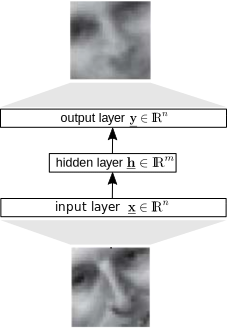
\includegraphics[width=4.25cm]{section1_fig52}
\end{figure}
\iitem{shallow ``auto-encoder'' to learn invariances/representations:
				\iitem{MLP output predicts input}
				\iitem{smaller hidden layer, i.e.~$m \ll n$}
		}
\begin{equation}
E^T_{[\vec w]} = \smallfrac{1}{p} \sum_{\alpha=1}^{p} 
	\smallfrac{1}{n} \smallsum{i=1}{n}
	\Big(y_i(\vec x^{(\alpha)}|\vec w) - x_i^{(\alpha)} \Big)^2
\end{equation}
\iitem{hidden layer $\vec h$ learns low-dimensional 
					representation/encoding of input}
\iitem{compact representations often {\em generalize} 
					better to unseen inputs}
\iitem{information bottleneck}				

%
\paragraph{Deep belief networks (DBN)}\mbox{}\\
\begin{figure}
\includegraphics[width=0.95\textwidth]{section1_fig53}
\end{figure}
Restricted Boltzmann Machines \citep{Hinton06b}: \\
\iitem{initialize parameters by layer-wise unsupervised pre-training}
\iitem{hidden units of each layer are the input to the next}
Encoding and Decoding\cite{Hinton06}:\\
\iitem{{\bf encoding}: compresses input to low-dimensional representation}
\iitem{{\bf decoding}: generates an input ``image'' from the representation }
Fine Tuning \cite{Hinton06}:\\
\iitem{{\bf generative auto-encoder} can be fine-tuned by back-propagation}
\iitem{learns an efficient representation of training set plus noise $\varepsilon_i$}

\paragraph{Mini-batch stochastic gradient descend}
Deep learning requires a large training set which may not fit in the memory. Therefore, the batch gradient descent is not feasible. On the other hand, the online stochastic gradient descent is very slow as it requires a very small learning rate. So, mini-batches are used for gradient updates which is a common practice. 
\iitem{\small asynchronously request small random 
					subsets of the data}
\iitem{\small update based on the average gradient of the mini-batch}
\iitem{\small faster convergence than online learning}

\paragraph{Layer-wise pre-training} (\cite{Bengio09})
\iitem{deep MLP with random initializations require very large training sets}
\iitem{layer-wise auto-encoder pre-training reduces the number of samples}

\subsubsection{Regularization for Deep Learning}
\paragraph{Norm regularization}
\iitem{all previously discussed regularization methods work, e.g.}
	\begin{align}
		\tag{$L_2$ regularization}
		R_{[\vec w]} \quad&=\quad \smallsum{i=1}{N} w_i^2 \\
		\tag{$L_1$ regularization}
		R_{[\vec w]} \quad&=\quad \smallsum{i=1}{N} |w_i|
	\end{align}
\begin{center}
	\includegraphics[width=7cm]{RegularizationTypesIntersect_clean.png}
\end{center}

\paragraph{Data augmentation}
\iitem{perform transformations on the training data}
	\begin{center}
		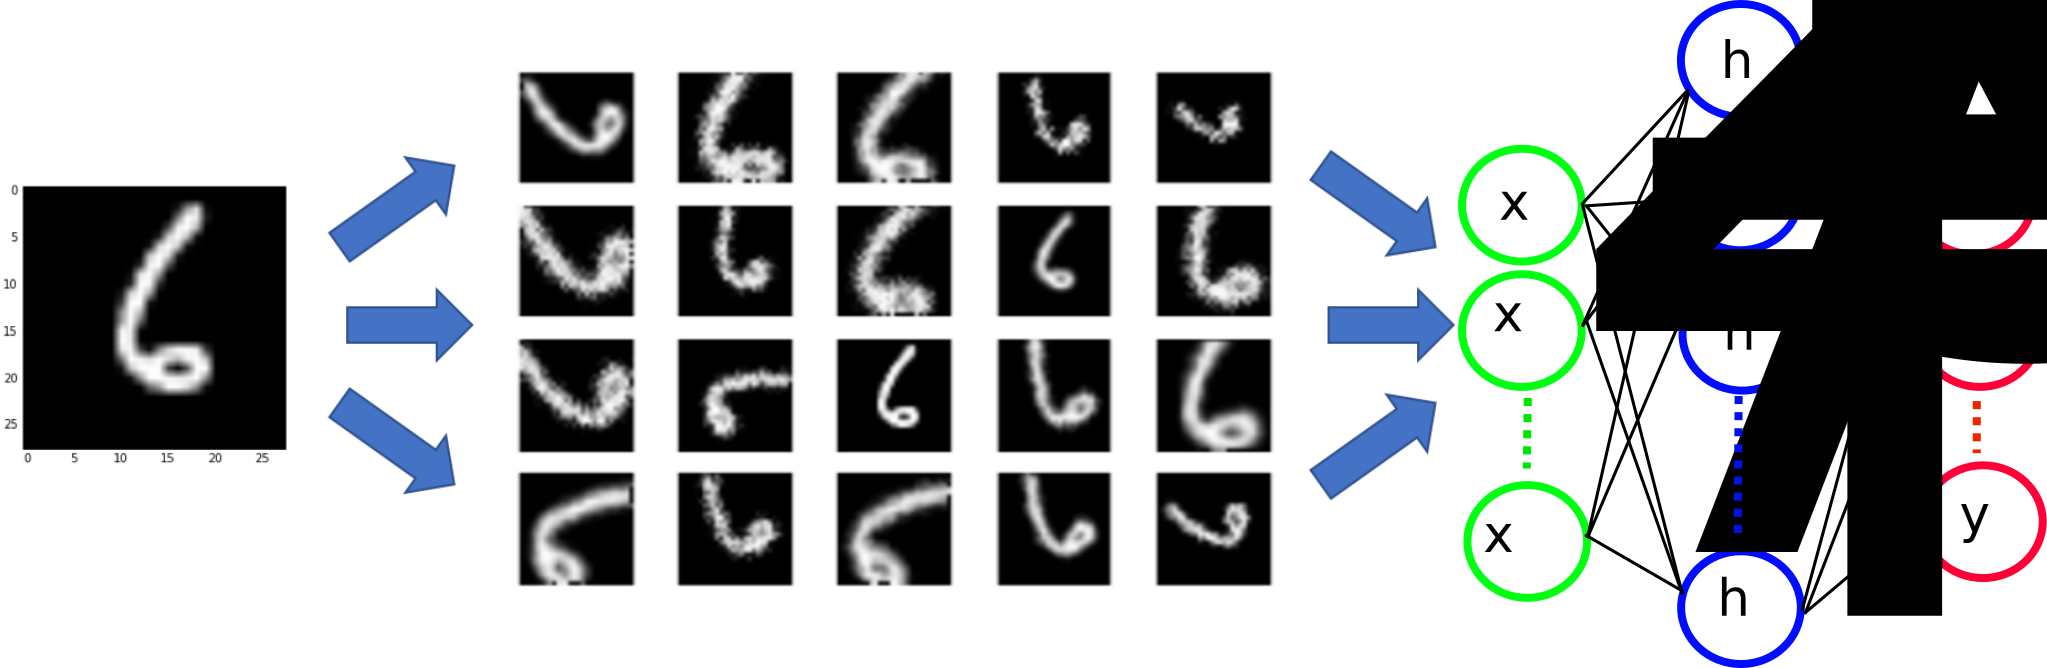
\includegraphics[width=11cm]{section1_fig55}
	\end{center}
\iitem{injecting noise in training samples and labels}
\iitem{output becomes {\em invariant} against transformations and noise}
\paragraph{Dropout}(\cite{Srivastava14})
\begin{center}
		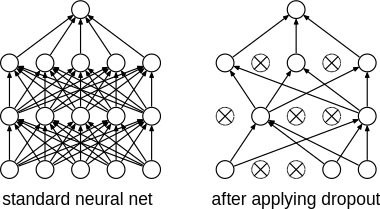
\includegraphics[height=4cm]{section1_fig56}
\end{center}
\iitem{each update step deactivates a number of randomly chosen neurons}
\iitem{prediction uses all neurons with proportionally scaled weights}
\iitem{Dropout as an ensemble method:
\begin{center}
		\includegraphics[height=4cm]{section1_fig57}
\end{center}}
\iitem{dropout updates an ensemble of $2^n$ models
			\iitem{ all models share parameters $\vec W$
			\item neurons $i$ are deactivated by 
			  		drawing $d_i \in \{0,1\}$ (Bernoulli i.i.d.)
			\item each neuron's output $S_i(\vec x)$ 
			  		is multiplied by $d_i \in \{0,1\}$
			\item each model can be identified by a unique 
			  		vector $\vec d \in \{0,1\}^n$
			}
		}

\iitem{ all probabilistic predictions are (geometrically) averaged
			\iitem{the distribution factorizes, i.e.~$P(\vec d) = \prod_i P(d_i)$}
		}

\iitem{approximation can rarely be proven, but works well empirically}
\begin{equation}
P(y|\vec x) \quad=\quad \sqrt[\leftroot{-2}\uproot{0}{2^n}]%
				{ {\textstyle\prod\limits_{\scriptscriptstyle\vec d \in \{0,1\}^n}} 
					\kern-1.5ex P(\vec d) \, P\big(y\,|\,\vec d \cdot \vec S(\vec x)\big) }
			\quad\approx\quad P\big(y\,|\, \E[\vec d] \cdot \vec S(\vec x)\big)
\end{equation}
\iitem{prediction uses all neurons, but scales the learned weights}
\begin{equation}
		w_{ij}^{v'v} \quad\leftarrow\quad w_{ij}^{v'v} \cdot \E[d_j^v] 
\end{equation}
\iitem{the prediction approximates the geometric ensemble average}
\slideref{Ex: MNIST results with dropout}
\subsubsection{Convolutional Layers}
\paragraph{Structured input and output}\mbox{}\\
	\begin{minipage}{12cm}
		\begin{minipage}{3.5cm}
			\vspace{12mm}
			\includegraphics[width=\textwidth]{soundwave.png}
			\vspace{2mm}
			\begin{center}
				$1 \times n$ \\[-2mm] tensor
			\end{center}
		\end{minipage}
		\hfill
		\begin{minipage}{2cm}
			\includegraphics[width=\textwidth]{pixels_marilyn.jpg} 
			\vspace{-4mm}
			\begin{center}
				$n \times m$ \\[-2mm] tensor
			\end{center}
		\end{minipage}
		\hfill
		\begin{minipage}{2cm}
			\vspace{4mm}
			\includegraphics[width=\textwidth]{pixels_marilyn_color_2.jpeg}
			\begin{center}
				$n \times m \times 3$ \\[-2mm] tensor
			\end{center}
		\end{minipage}
		\hfill
		\begin{minipage}{3.4cm}
			\vspace{1mm}
			\includegraphics[width=\textwidth]{pixels_moving_object.png}
			\begin{center}
				$n \times m \times 3 \times t$ \\[-2mm] tensor
			\end{center}
		\end{minipage}
	\end{minipage}
\iitem{structured input/output spaces are sometimes called \textbf{tensors} 
\iitem{here defined as multidimensional extensions of matrices} 
\iitem{tensors imply a {\em spatial} relationship between variables}}
\iitem{MLP can have tensors as inputs and as outputs, e.g.
			\iitem{MNIST has a $28 \times 28$ input tensor
				and a $10 \times 1$ output vector}
			%\vspace{1mm}\hspace{4cm}
			%\includegraphics[width=3cm]{img/mnist_single_tensor.png}
			\iitem{segmentation to predict the location of $c$ object-classes in an image\\
				has a $n \times m \times 3$ input tensor 
				and a $n \times m \times c$ output tensor}
			%\vspace{1mm}\hspace{34mm}
			%\includegraphics[width=4.2cm]{img/image_segmentation_example.pdf}
		}

\paragraph{Convolutions}
\iitem{convolutions require a spatial structure, i.e.~an input tensor}
\iitem{Example: one-dimensional audio data
\begin{figure}[h]
\centering
\includegraphics[width=0.5\textwidth]{section1_fig69}
\end{figure}
	\iitem{$\vec x$ is a $1 \times n$ input tensor
						\vspace{-1mm}
					  	\item $\vec w$ is a $1 \times n'$ filter tensor
					  	\vspace{-1mm}
					  	\item $\vec h$ is a $1 \times
					  			(n {\kern-0.5ex} - {\kern-0.5ex} n')$ output tensor
			}
	}	
\vspace{-0.5cm}
\begin{eqnarray*}
		h_i \;\;=\;\; (\vec x * \vec w )_{(i)}
		&=& \sum_{k=1}^{n-n'} \, x_k \; w_{i-k} 
		\;\;=\;\; \sum_{k=1}^{n'} \, x_{i-k} \; w_{k} 
		\qquad \text{(convolution)}\\
		h_i \;\;=\;\; (\vec x \star \vec w)_{(i)}
		&=& 
		\sum_{k=1}^{n-n'} \, x_k \; w_{i+k} 
		\;\;=\;\; \sum_{k=1}^{n'} \, x_{i+k} \; w_{k} 
		\qquad \text{(correlation-> subtle difference)}
	\end{eqnarray*}	
\iitem{Example: two-dimensional gray-scale images
\begin{figure}[h]
\centering
\includegraphics[width=0.5\textwidth]{section1_fig70}
\end{figure}
					\iitem{$\vec X$ is a $n \times m$ input tensor
						\vspace{1mm}
					  	\item $\vec W$ is a $n' \times m'$ filter tensor
					  	\vspace{1mm}
					  	\item $\vec H$ is a $(n\kern-.5ex-\kern-.5exn') 
					  		\times (m\kern-.5ex-\kern-.5ex m')$ output tensor
					}
				}
\begin{eqnarray*}
			\vec H_{(i,j)} \quad=\quad (\vec X * \vec W )_{(i,j)}
			&=& \sum_{k=1}^n \sum_{l=1}^m \, \vec X_{(k,l)} \; \vec W_{(i-k, j-l)} \\
			&=& \sum_{k=1}^{n'} \sum_{l=1}^{m'} \, \vec X_{(i-k,j-l)} \; \vec W_{(k, l)}
		\end{eqnarray*}	

\paragraph{Convolutions reduce number of parameters}
	\iitem{convolutions correspond to a sparsely connected shared weight matrix}
	\begin{center}
		\includegraphics[width=7cm]{section1_fig71}
	\end{center}
	\vspace{-3mm}
	\iitem{sparse shared weight matrix $\vec W \in \R^{n \times n-n'}$ has only $n'$ parameters}
	\vspace{-1mm}
	\iitem{shifted filters enforce a location-invariant feature}

\paragraph{Feature maps}
	\iitem{most tasks require multiple features, 
		e.g.~horizontal and vertical edges}
	\begin{center}
		\includegraphics[width=10cm]{section1_fig72}
	\end{center}
	\vspace{-2mm}
	\iitem{$n \times m \times 3$ input tensor $\longrightarrow$ 
		$(n-3) \times (m-3) \times 2$ output tensor}

\paragraph{Convolutional layers in MLP}
\begin{center}
		\includegraphics[width=8cm]{section1_fig73}
	\end{center}
	\vspace{-2mm}
	\iitem{convolutional layer gets {\color{blue}activities $h_i^v$} 
			from the preceding layer}
	\vspace{-1mm}
	\iitem{convolutional layer gets {\color{red}errors $\delta_j^{v'}$} 
			from the succeeding layer}
\paragraph{Training convolutional layers}
	\begin{enumerate}			
\item gradient calculation by chain rule:\\[-2mm]
			$\displaystyle 
				\smallfrac{\partial {\color{red}e^{(\alpha)}}}
					{\partial w_{k}^{v}}
				\quad=\quad 
					\smallsum{j=1}{n-n'}
					\smallfrac{\partial{\color{red} e^{(\alpha)}}}
						{\partial {\color{blue}h_j^{v'}}}
					\cdot \smallfrac{\partial {\color{blue}h_j^{v'}}}
						{\partial w_{k}^{v}}
				\quad=\quad
					\Big[ \overbrace{ 
						\smallfrac{\partial {\color{red}e^{(\alpha)}}}%
						{\partial {\color{blue}\vec h^{v'}}} 
					}^{\kern-2ex{\color{red}\text{error}\,\vec \delta^{v'}}\kern-2ex} 
					\star \underbrace{
						f\big({\color{blue}\vec h^{v}}\big)
					}_{\kern-2ex\color{blue}\text{activity}\,\vec h^v\kern-2ex} 
					\Big]_{(n'-k)}
			$	
		\item forward pass:
			$$
				{\color{blue}h_j^{v'}}
				\;:=\; [ f({\color{blue}\vec h^v}) * \vec w^{v} ]_{(j)}
				\;=\; \smallsum{k=1}{n'} f\big({\color{blue}h^{v}_{n'+j-k}}\big) 
					\cdot w_k^v  \,,
				\qquad \forall j \in \{1, \ldots, n-n'\}
			$$	
		\vspace{0mm}	
		\item backward pass: \\[3mm]
			$\displaystyle 
				{\color{red}\delta_i^{v}}
				\quad=\quad 
					f'\big( {\color{blue}h_i^{v}} \big) \cdot
					\big[ {\color{red}\vec \delta^{v'}} \star \vec w^{v} 
					\big]_{(i-n')}
				\quad=\quad 
					f'\big( {\color{blue}h_i^{v}} \big) \cdot
					\smallsum{j=1}{n'}
					{\color{red} \delta_{(i-n')+j}^{v'} }
					\cdot w_j^v  
			$
			%\hfill
			%(note the cross-correlations $\star$)
	\end{enumerate}			
\paragraph{Training convolutional layers: derivation}			
\iitem{forward pass:}
	$$
		{\color{blue}h_j^{v'}}
		\;:=\; [ f({\color{blue}\vec h^v}) * \vec w^{v} ]_{(j)}
		\;=\; \smallsum{k=1}{n'} f\big({\color{blue}h^{v}_{n'+j-k}}\big) 
			\cdot w_k^v  \,,
		\qquad \forall j \in \{1, \ldots, n-n'\}
	$$
	\vspace{4mm}
	\begin{minipage}{\textwidth} \footnotesize
		\begin{minipage}[t]{5.25cm}
			\iitem{gradient calculation:}
			\vspace{-4mm}
			\begin{eqnarray*}
				\smallfrac{\partial {\color{red}e^{(\alpha)}}}
					{\partial w_{k}^{v}}
				&=& \smallsum{j=1}{n-n'}
					\smallfrac{\partial{\color{red} e^{(\alpha)}}}
						{\partial {\color{blue}h_j^{v'}}}
					\cdot \smallfrac{\partial {\color{blue}h_j^{v'}}}
						{\partial w_{k}^{v}} \\
				&=& \smallsum{j=1}{n-n'}
					\smallfrac{\partial {\color{red}{e^{(\alpha)}}}}%
						{\partial {\color{blue}h_j^{v'}}}
					\cdot f\big({\color{blue}h^{v}_{n'+j-k}}\big) \\
				&=& \Big[ \underbrace{ 
						\smallfrac{\partial {\color{red}e^{(\alpha)}}}%
						{\partial {\color{blue}\vec h^{v'}}} 
					}_{{\color{red}\vec \delta^{v'}}} 
					\star \underbrace{
						f\big({\color{blue}\vec h^{v}}\big)
					}_{\text{\color{blue}input}} \Big]_{(n'-k)}
			\end{eqnarray*}		
		\end{minipage}
		\hfill
		\begin{minipage}[t]{5.5cm}
			\iitem{backward pass:}
			\vspace{-4mm}
			\begin{eqnarray*}
				{\color{red}\delta_i^{v}}
				&=& \smallsum{j=1}{n-n'}
					\smallfrac{\partial {\color{red}e^{(\alpha)}}}%
						{\partial {\color{blue}h^{v'}_j}}
					\cdot \smallfrac{\partial {\color{blue}h_j^{v'}}}
						{\partial f({\color{blue}h_i^{v}})}
					\cdot \smallfrac{\partial f({\color{blue}h_i^{v}})}
						{\partial {\color{blue}h_i^{v}}} \\
				&=& \smallsum{j=1}{n-n'}
					{\color{red}\delta_j^{v'}}
					\cdot w^{v}_{n'+j-i}
					\cdot f'\big( {\color{blue}h_i^{v}} \big) \\
				&=& \smallsum{j=1}{n'}
					{\color{red}\delta_{i-n'+j}^{v'}}
					\cdot w^{v}_{j}
					\cdot f'\big( {\color{blue}h_i^{v}} \big) \\
				&=& \big[ {\color{red}\vec \delta^{v'}}  
							\star \vec w^{v} 
						\big]_{(i-n')}
					\cdot f'\big( {\color{blue}h_i^{v}} \big)
			\end{eqnarray*}				
		\end{minipage}
	\end{minipage}
	\iitem{note that gradient and backward-pass are computed with a correlation}			
\subsubsection{Convolutional Architectures}
\definecolor{midred}{rgb}{0.75,0,0}
\definecolor{darkgreen}{rgb}{0,0.5,0}
\begin{center}
		\includegraphics[width=12cm]{section1_fig74}
	\end{center}
	\iitem{most modern deep architecture consist of:
		\vspace{1mm}
		\iitem{a larger number of {\color{blue}convolutional layers} 
				(increase \#features)}
		\vspace{0mm}
		\iitem{{\color{darkgreen}pooling and down-sampling layers} (decrease size)}
		\vspace{-1mm}
		\iitem{a smaller number of {\color{midred}fully connected layers}}
	}

\paragraph{Introducing invariances: spatial pooling}
	\iitem{invariance to small spatial transformation, e.g.}
	$$
		f_i(\vec x) = \max(x_{i-m}, x_{i-m+1}, \ldots, x_{i+m-1}, x_{i+m})
		\hspace{10mm}
	$$
\begin{center}
		\includegraphics[width=12cm]{section1_fig75} \\[2mm]
		\includegraphics[width=12cm]{section1_fig76}
\end{center}
\paragraph{Down-sampling}\mbox{}\\
\iitem{spatial invariance (from pooling) can be exploited by down-sampling
		\iitem{using only every {\color{blue}\em stride}'th output node, 
				e.g.~for {\color{blue} stride 2}:}}
	\begin{center}
		\includegraphics[width=12cm]{section1_fig77}
	\end{center}
	
\iitem{down-sampling yields more compact representation
		\vspace{1mm}
		\iitem{smaller output tensors $\leadsto$ less parameters in successive layers}}

\paragraph{Introducing invariances: feature pooling}\citep[maxout networks,][]{Goodfellow13a}
	\iitem{other invariances can be learned by pooling over multiple features
		\iitem{each filter learns to detect the feature in another pose}
		\iitem{the pooling layer keeps the maximum of the participating filters}
		\iitem{the pooled output is invariant against the learned transformation}}
	\begin{center}
		\centering
		\includegraphics[height=4cm]{section1_fig78}
	\end{center}
	\iitem{training determines which invariances are learned}

\paragraph{Input tensors with varying size}
\iitem{images come in many sizes and resolutions
		\vspace{1mm}
		\iitem{but fully connected layers have a fixed input size}
		\iitem{convolution is size-free and downsampling strides are flexible}}
\begin{figure}[h]
\centering
\includegraphics[width=7cm]{maxpooling_images.png}
\end{figure}
\iitem{one can exploit {\em downsampling} to reduce the image size 
		\iitem{choose {\em stride} in each layer such that the input 
			size \\ of the first fully connected layer is constant}}
\begin{figure}[h]
\centering
\includegraphics[width=7cm]{section1_fig79}
\end{figure}
\paragraph{Depth and parameter sizes}
\begin{center}
		\includegraphics[width=10cm]{deep_full_vs_convolutional.png}\\
		\small house-number recognition on street-view images \citep{Goodfellow14d}
	\end{center}
	
	\iitem{ convolutions {\em reduce parameters}, which allows for more layers
	  \item convolutions {\em regularize} by restricting the model class
	  \item convolutions {\em generalize} better due to introduced invariances
	}
\paragraph{Example deep architecture: detecting traffic signs}

		\iitem{detection of speed related traffic signs for a fixed input size
			\vspace{2mm}
			\iitem{small $32 \times 32$ input images of traffic signs}
			\vspace{1mm}
			\iitem{three $5 \times 5$ convolution layers 
					with $2 \times 2$ downsampled max-pooling}
			\iitem{each convolution layer increases the features,
					but reduces the size}
			\iitem{one fully connected layer predicts the traffic sign}
		}
		\vspace{2mm}
		\begin{center}
			\includegraphics[width=11cm]{section1_fig80.pdf}
		\end{center}
		\vspace{-4mm}
	
		\iitem{simultaneous detection of speed limits and traffic sign position
			\vspace{2mm}
			\iitem{apply sign-recognition network on every 
					{\em tile} of a $720 \times 1280$ image
			\vspace{2mm}
			\item  each application predicts which traffic sign is present in the tile
			\vspace{2mm}
			\item  final map detects all visible traffic signs and their position}
		}
		\begin{center}
			\includegraphics[width=12cm]{section1_fig81.pdf}
		\end{center}
		\vspace{-2mm}
		\iitem{network runs real-time on customized hardware (e.g.~in a car)}

\paragraph{Deconvolutional networks}	
\begin{figure}[h]
		\centering
		\includegraphics[width=10cm]{deconvolution_network.png} 
		\caption{Deconvolutional networks \cite{Noh15}}
\end{figure}
			\iitem{MLP output tensors can be equal (or larger) than the input tensor
				\vspace{1mm}
				\iitem{e.g.~image segmentation: identify which pixel belongs to which object}
			}
			\vspace{4mm}
			\iitem{original convolution and pooling layers must be {\em reversed}
				\vspace{1mm}
				\iitem{deconvolutional (sub-)networks have larger output tensors}
			}

\paragraph{Unpooling layers}
\iitem{every pooling layer can be reversed by an unpooling layer}
			\iitem{remember ``switch-variables'', i.e.~which unit was maximal}
			\iitem{yields enlarged, but sparse feature maps}
\begin{figure}[h]
\centering
\includegraphics[width=7cm]{section1_fig82}
\caption{Unpooling layers \cite{Noh15}}
\end{figure}

\paragraph{Deconvolutional layers}
\iitem{every convolution layer can be reversed by a deconvolution layer}
			\iitem{learns small input tensors \\ to predict large output tensors}
			\iitem{convolution generates dense feature maps
					from sparse unpooling maps}	
\begin{figure}[h]
\centering
\includegraphics[width=7cm]{section1_fig83}	
\caption{Deconvolutional layers \cite{Noh15}}
\end{figure}	

\begin{figure}[h]
\centering
\includegraphics[width=10cm]{section1_fig84} 
\caption{Deconvolutional example: image segmentation}
\small trained on PASCAL VOC 2012 benchmark data \cite{Noh15}
\end{figure}

\subsection{Recurrent Networks}
\subsubsection{Time series}	
\iitem{sequences of samples of arbitrary/varying length $n$
		\iitem{generated by a dynamic system evolving in time e.g. speech, video}}
	\iitem{time series prediction:
		\iitem{predict the next $m$ samples
		\item  {based on the last $n$ samples e.g. predict share price in stock-exchange}}}
	\iitem{time series generation:
		\iitem{generate a new time series 
		\item  conditioned on a sequence or image in another format} \slideref{Ex: more time series on slide}}
\paragraph{Time series distributions}
\begin{figure}[h]
	\begin{subfigure}{0.49\textwidth}
	\includegraphics[width=\textwidth]{section1_fig59}
	\caption{Time series with no window}
	\end{subfigure}
	\begin{subfigure}{0.49\textwidth}
	\includegraphics[width=\textwidth]{section1_fig60}
	\caption{Time series with finite window}
	\end{subfigure}
	\caption{Time series distribution}\label{fig:time_series_windows}
\end{figure}
\iitem{probability at each time step depends on all previous observations (\ref{fig:time_windows})}
	$$
		P\Big( \vec y^{(t)} | \vec y^{(1)}, \ldots, \vec y^{(t-1)} \Big)
	$$

\iitem{we assume often the {\color{blue}distribution} 
			depends on a short {\color{green}time-window}(\ref{fig:time_windows})}
		$$
			P\Big({\color{blue}\vec y^{(t)}}|
				{\color{green}\vec y^{(t-m)}, \ldots, \vec y^{(t-1)}}\Big)
		$$
\slideref{Ex: Time series exmaples on slide}

\paragraph{Modeling time series with hidden states}
$ P\big(\vec y^{(t+1)} | \vec y^{(1)}, \ldots, \vec y^{(t)}\big) 
		\approx P\big( \vec y^{(t+1)} | \vec h^{(t)} \big)$\\
\begin{figure}
	\centering
	\includegraphics[width=0.5\textwidth]{section1_fig61}
	\caption{Modeling time series with hidden states}\label{fig:time_series_model}
\end{figure}

\subsubsection{Recurrent Networks}
\paragraph{Recurrent neural networks (RNN)}
\begin{figure}
	\begin{subfigure}{0.65\textwidth}
	\centering
	\includegraphics[width=0.75\textwidth]{section1_fig62}
	\end{subfigure}
	\begin{subfigure}{0.29\textwidth}
	\centering
	\includegraphics[width=0.75\textwidth]{section1_fig63}
	\end{subfigure}
	\caption{Recurrent neural networks (RNN)}\label{fig:rnn}
\end{figure}
From Figure \ref{fig:rnn}, the hidden states and output can be written as, 
\begin{eqnarray*}
			h_i^{(t)} &=& f\Big({\color{blue}\smallsum{k=1}{N} U_{ik} \, x_k^{(t)}} 
					{{\color{red} + \smallsum{j=1}{H} 
							W_{ij} \, h_j^{(t-1)}}}
					+ b_i \Big) \,,
				\qquad\text{e.g.}\;f(\cdot) = \tanh(\cdot)\\
			y_k^{(t)} &=& g\Big({\color{green}\smallsum{j=1}{H} 
					V_{kj} \, h_j^{(t)}} + c_k\Big) \,,
				\hspace{28mm}\text{e.g.}\;g(\cdot) = \text{\rm softmax}(\cdot)
\end{eqnarray*}
\iitem{generates an output $\vec y^{(t)}$ at each time step $t$}
\iitem{takes an input $\vec x^{(t)}$ at each time step $t$
\iitem{possibly previous output $\vec y^{(t-1)}$}}
\iitem{summarizes all previous inputs as $\vec h^{(t)}$}
\iitem{one hidden layer is sufficient \\[0mm]
{\footnotesize(hidden layer is universal approximator)}}

\paragraph{RNN are Turing machines}
\iitem{Turing machines (TM) are theoretical computing machines
		\vspace{1mm} 
		\iitem{TM apply a finite set of operations between a number of {\em stacks}
		 \vspace{1mm}
		 \item TM can compute any recursively computable function $\phi: \N \to \N$}}
\iitem{RNN are universal Turing Machines \cite{Siegelmann91}} 

\iitem{input sequence $x_1^{(t)}$ contains 
				function $\phi$ and parameter $n$}
			\vspace{-3mm}
			\iitem{transfer functions encode the binary size of stacks
				$f(\cdot) = g(\cdot) = \min\big( \max(\cdot, 0), 1\big)$
				\vspace{-2mm}
				\iitem{binary $n = 1011...$ 
					are represented $h_i^{(t)} = 0.1011...$}}
			\vspace{-4mm}
			\iitem{all operations of a TM can be encoded by weights}
			\vspace{-4mm}
			\iitem{output sequence $y_1^{(t)}$ contains answer $m = \phi(n)$}
				\vspace{-3mm}
				$$
					y_1^{(\ldots)} = 0\ldots 0%
					\overbrace{1\ldots 1}^{m\text{ times}}0\ldots
				$$

\clearpage
\paragraph{Training an RNN}
\begin{figure}[h]
	\begin{subfigure}{0.25\textwidth}
	\centering
	\includegraphics[width=0.8\textwidth]{section1_fig64}
	\end{subfigure}
	\begin{subfigure}{0.65\textwidth}
	\centering
	\includegraphics[width=\textwidth]{section1_fig65}
	\end{subfigure}
	\caption{Training an RNN}\label{fig:training_rnn}
\end{figure}
\begin{itemize}
		\item cost function $e^{(\alpha,t)}$ for time 
				step $t$ of training sequence $\alpha$ 
			$$
				E^T = \smallfrac{1}{p} \sum\limits_{\alpha=1}^p
				\smallfrac{1}{n_\alpha}\smallsum{t=1}{n} e^{(\alpha,t)} \,,
				\quad \text{for training set} \quad 
				\Big\{ \{ \vec x^{(\alpha,t)}, \vec y^{(\alpha,t)} 
					\}_{t=1}^{n_\alpha}\Big\}_{\alpha=1}^{p}
			$$
		\item compute gradient of a sequence by unfolding the network in time 
		\item online gradient computation for sequence $\alpha$
			has complexity $\Set O(n_\alpha^2)$
	\end{itemize}
\paragraph{Backpropagation through time (BPTT)}
\begin{figure}
	\centering
	\includegraphics[width=0.65\textwidth]{section1_fig67}
	\caption{Backpropagation through time (BPTT)}\label{fig:rnn_bptt}
\end{figure}
\begin{itemize}
		\item assume all unfolded weights, 
				e.g.~$\color{blue}\vec W^{(t)}$, are independent
		\item compute gradients of deep MLP with backpropagation 
				($\leadsto \Set O(n_\alpha)$)
		\item average all computed gradients 
				${\color{blue} \frac{\partial e^{(\alpha,t)}}%
				{\partial \vec W^{(\alpha,\tau)}}}$ 
				for weight update
			$$ \hspace{-5mm}
				\Delta \vec W \;\; = \;\;
					-\eta \, \smallfrac{\partial E^T}{\partial \vec W}
				\;\;=\;\; -\smallfrac{\eta}{pn} 
					\smallsum{\alpha=1}{p} \smallsum{t=1}{n}
					\smallfrac{\partial e^{(\alpha, t)}}{\partial \vec W}
				\;\;\approx\;\; \smallfrac{\eta}{pn^2}
					\smallsum{\alpha=1}{p} \smallsum{t=1}{n} \smallsum{\tau=1}{n}
					{\color{blue} \smallfrac{\partial e^{(\alpha,t)}}%
						{\partial \vec W^{(\alpha,\tau)}}}
			$$
	\end{itemize}
\subsubsection{Long-term Dependencies}

\paragraph{Long-term Dependencies}
\iitem{long sequences require often a long memory}\slideref{Ex: Protein folding}\slideref{Ex: Text understanding}
\iitem{a RNN with no inputs and a linear transfer function}
	\vspace{1mm}
\begin{equation}
	\vec h^{(t)} 
	\quad = \quad \vec W \, \vec h^{(t-1)}
	\quad=\quad (\vec W)^t \, \vec h^{(0)}
\end{equation}
\iitem{eigenvalue decomposition:
		$\vec W = \vec U \, \vec \Lambda \, \vec U^\top$}
\begin{equation}
\vec h^{(t)} \quad =\quad 
			\underbrace{\vec U
			}_{\kern-3ex\text{\footnotesize rotate back}\kern-3ex}
			\overbrace{(\vec \Lambda)^t
			}^{\kern-6ex\text{\footnotesize exponential scaling}\kern-6ex}
			\underbrace{\vec U^\top \vec h^{(0)}
			}_{\text{\footnotesize rotation}}
\end{equation}
\iitem{long-term activity dominated by the largest $|\lambda_{1}|$ 
\iitem{$|\lambda_{1}| > 1 \quad 
			\leadsto \quad \lim\limits_{t\to\infty} h_i^{(t)} = \pm \infty\,,
				\forall i$
			\hfill (exploding activity)}
		\vspace{-2mm}
		\iitem{$|\lambda_{1}| < 1 \quad 
			\leadsto \quad \lim\limits_{t\to\infty} h_i^{(t)} = 0 \,,
				\forall i$
			\hfill (vanishing activity)}
	}
\paragraph{Vanishing gradients}
\iitem{local error terms $\vec \delta^{(t)}$ in backpropagation through time
		\vspace{1mm}
		\iitem{for transfer function $f(x) = \tanh(x)$, 
				i.e.~$f'(x) = \big(1 - f^2(x)\big)$}}
	$$
		\delta_i^{(t)} 
		\quad=\quad \smallfrac{\partial E^T}{\partial h_i^{(t)}}
		\quad=\quad \Big(\kern-1.5ex\underbrace{1 - \big(h_i^{(t)}\big)^2
				}_{\begin{array}{c}\\[-4mm]
					\text{\scriptsize derivative < 1} \\[-1.5mm]
					\text{\scriptsize i.e.~contracting} 
				\end{array}} \kern-1.5ex\Big)
			\cdot \Big(\underbrace{\smallsum{j=1}{H} W_{ij}^\top \delta_j^{(t+1)}
				}_{\kern-2ex\begin{array}{c}\\[-6mm]
					\text{\scriptsize potentially} \\[-1.75mm]
					\text{\scriptsize exploding/vanishing}
				\end{array}\kern-2ex}\Big)
	$$
	\iitem{over many time steps the local errors $\delta_i^{(t)}$ often vanish}
		%\vspace{1mm}
		%\iitem{large $\vec w_i \Rightarrow h_i^{(t)} \approx 1 \Rightarrow$ 
		%	derivative $\approx 0$}
		%\iitem{rarely explodes thanks to anti-cyclical derivative $<1$}
	\iitem{small short-term errors overshadow large long-term errors}

\paragraph{Solution 1: echo-state networks}\citep[Section 10.8]{Jaeger04,Goodfellow16}
\iitem{system dynamics determine the input representation
	\iitem{non-linear preprocessing step with memory}}
\iitem{address vanishing gradients by keeping $\vec W$ and $\vec U$ fixed
	\iitem{output weights $\vec V$ can be trained by e.g.~linear regression}
	\iitem{hidden ``reservoir'' maintains inputs/errors over time}
	}
\iitem{system dynamics determine how fast inputs/errors are forgotten}
\iitem{eigenvalues $\lambda_i$ of the system's {\em Jacobian} $\vec J$}
			$$
				J_{ij}^{(t)} 
				\quad=\quad 
				\smallfrac{\partial h_i^{(t)}}{\partial h_j^{(t-1)}}
				\quad=\quad
				f'\big(h_i^{(t)}\big) \cdot W_{ij}
				\hspace{2cm}
			$$
\iitem{eigenvectors with $|\lambda_i| \approx 1$ vanish/explode {\em very slowly}
	\iitem{inputs/errors are maintained for a long time}}
\iitem{generate random $\vec W$, and $\vec U$ 
				where all $|\lambda_i| \approx r$
		\iitem{$f'(h_i^{(t)}) < 1$ \quad is a contraction $\quad\leadsto\quad$ $r > 1$}
		\iitem{values between $r=1.2$ and $r=3$ are used in practice}
		\iitem{$n$ hidden neurons can maintain
					inputs/errors for up to $n$ time steps }
		}

\paragraph{Solution 2: leaky units \citep[Section 10.9]{Goodfellow16}}
\begin{wrapfigure}{r}{0.15\textwidth}
  \begin{center}
    \includegraphics[scale=0.9]{section1_fig68}
  \end{center}
  \caption{Leaky unit}
\end{wrapfigure}
\iitem{introduce linear ``leaky units'' $\mu_i$}
	$\qquad
		\mu_i^{(t)} \quad=\quad
		\alpha_i \, \mu_i^{(t-1)} + (1-\alpha_i) \, h_i^{(t-1)} \,,
		\qquad 0 < \alpha_i < 1
	$

	\iitem{$\mu_i$ estimates the average activity of $h_i$
			with time constant $\alpha_i$
		\iitem{averages maintain errors/activity over longer time periods}
		\iitem{small $\alpha_i$ average over short periods}
		\iitem{large $\alpha_i$ average over long periods}}
	\iitem{leaky unit's have different time constants $\alpha_i$}
\iitem{introduce linear ``leaky units'' $\mu_i$}
	$\qquad
		\mu_i^{(t)} \quad=\quad
		\alpha_i \, \mu_i^{(t-1)} + (1-\alpha_i) \, h_i^{(t-1)} \,,
		\qquad 0 < \alpha_i < 1
	$
	\vspace{6mm}
	\iitem{the extended system's Jacobian $\vec J_{h\mu}$:}
	\vspace{2mm}
	{\small $$
		\vec J_{h\mu} 
		\;\;=\;\;
		\mat{\partial \vec h^{(t)} / \partial \vec h^{(t-1)}, & 
			\partial \vec h^{(t)} / \partial \vec\mu^{(t-1)} \\ 
			\partial \vec\mu^{(t)} / \partial \vec h^{(t-1)}, &
			\partial \vec\mu^{(t)} / \partial \vec\mu^{(t-1)}}
		\;\;=\;\; 
		\mat{\vec J_h\quad, & \vec 0 \\ 
			\text{diag}(1-\vec\alpha)\,, & \text{diag}(\vec \alpha)}
	$$}
	\vspace{2mm}
	\iitem{errors/inputs in $\mu_i$ vanish with eigenvalue $\alpha_i$
		\vspace{1mm}
		\iitem{pairs $h_i/\mu_i$ with small $\alpha_i$ 
				specialize in {\em short-term memory}}
		\vspace{-1mm}
		\iitem{pairs $h_i/\mu_i$ with large $\alpha_i$ 
				specialize in {\em long-term memory}}}

\paragraph{Leaky units with indefinite memory?}
\iitem{unit $\mu_i$ with $\alpha_i=1$ 
		\vspace{1mm}
		\iitem{$\mu_i$	would maintain memories indefinitely}
		\vspace{-1mm}
		\iitem{$\mu_i$ can no longer be overwritten by the accompanying $h_i$}
	}
\iitem{BPTT sends local errors $\delta_i'^{(t)}$ in an endless loop
$$\hspace{-6mm}
			\delta_i'^{(t)} 
			\quad:=\quad \smallfrac{\partial E^T}{\partial \mu_i^{(t)}}
			\quad=\quad {\color{red}\delta_i'^{(t+1)}} + \smallsum{k=1}{M} 
				\smallfrac{\partial E^T}{\partial y_k^{(t)}} 
				\cdot V'_{ki} \cdot f'\big(\smallsum{j=1}{H} V_{kj} \, h_j^{(t)}
					+ \smallsum{l=1}{L} V'_{kl} \, \mu_l^{(t)}\big)
		$$
		\iitem{local errors from the output nodes $y_k^{(t)}$ 
				{\color{red}accumulate} in $\mu_i^{(t)}$ over time}
		\iitem{the accumulated error $\delta_i^{(t)}$ 
			never leaves $\mu_i$, due to $1-\alpha_i = 0$}
}
\iitem{memory units require a gating mechanism 
		\vspace{1mm}
		\iitem{for reading, writing and error handling}
	}

\paragraph{Solution 3: long short-term memory (LSTM)\citep[Section 10.10]{Hochreiter97,Goodfellow16}}
			\iitem{leaky unit $s_i$ with $\alpha_i=1$}
			\iitem{{\color{green}time delayed feedback} to hidden layer}
			\iitem{{\color{blue} transfer function} 
					$\sigma(x) = \big( 1 + e^{-x} \big)^{-1}$}
	\iitem{introducing an {\color{blue}input (``write'') gate 
					$g_i^\mathrm{i}$}
					\vspace{-2mm}
					\iitem{\footnotesize gate transfer function
							$\sigma(x) = \big( 1 + e^{-x} \big)^{-1}$} }
			\iitem{state input is multiplied ($\color{blue}\otimes$) with gate}
\newpage
\subsubsection{Recurrent Architectures}
\paragraph{Output recurrence}\citep[Section 10.2.1]{Goodfellow16}
\begin{figure}[h]
	\begin{subfigure}{0.22\textwidth}
	\includegraphics[width=\textwidth]{section1_fig85}
	\end{subfigure}
	\begin{subfigure}{0.69\textwidth}
	\includegraphics[width=\textwidth]{section1_fig86}
	\end{subfigure}
	\caption{Output recurrence}
\end{figure}

\begin{itemize}
		\item The activity of the hidden neurons depends on the previous output
		\item less powerful function class than general RNN 
		\iitem{but faster training procedure}
\end{itemize}
\paragraph{Teacher forcing}
	\iitem{replace $\vec y^{(t-1)}$ with $\vec y_T^{(t-1)}$ during training
			\iitem{each time step is independent and can be sampled i.i.d.}}
	%\iitem{forcing induces different training and test distributions
	%		\iitem{use mixture of real outputs and labels during training}}
	\iitem{training becomes robust when real outputs and labels are mixed}
\begin{figure}[h]
	\begin{subfigure}{0.22\textwidth}
	\includegraphics[width=\textwidth]{section1_fig85}
	\end{subfigure}
	\begin{subfigure}{0.69\textwidth}
	\includegraphics[width=\textwidth]{section1_fig88}
	\end{subfigure}
	\caption{Teacher forcing}
\end{figure}

\paragraph{Conditional sequences}
	\begin{itemize}
		\item all teacher forced time steps are {\em conditioned} 
				on the same input $\vec x$
		\vspace{2mm}
		\item the generated sequence can e.g.~describe the input $\vec x$
	\end{itemize}
\begin{figure}[h]
	\begin{subfigure}{0.22\textwidth}
	\includegraphics[width=\textwidth]{section1_fig64}
	\end{subfigure}
	\begin{subfigure}{0.69\textwidth}
	\includegraphics[width=\textwidth]{section1_fig89}
	\end{subfigure}
	\caption{Conditional sequences}
\end{figure}
\slideref{Ex: Image Description}

\paragraph{Bidirectional RNN \citep[Section 10.3]{Schuster97,Goodfellow16}}\mbox{}\\
\vspace{0.5cm}
	\begin{minipage}{\textwidth}
			\iitem{tasks like speech recognition and 
					translation are {\em context sensitive}
				\vspace{1mm}
				\iitem{the end of a sentence may be 
					as important as the beginning} }
		\begin{minipage}{6cm}
			\iitem{RNN evolve in one direction}
			\iitem{bidirectional RNN propagate information in {\em both} directions}
			\iitem{training as before with BPTT}
			\vspace{6mm}
		\end{minipage}
		\hfill
		\begin{minipage}{5.5cm}
			\includegraphics[width=\textwidth]{section1_fig90}
		\end{minipage}
	\end{minipage}
\slideref{Ex: Handwriting generation}	


\paragraph{Sequence-to-sequence architectures \citep[Section 10.4]{Goodfellow16}}\mbox{}\\
	\iitem{some tasks must be conditioned on sequences
		\iitem{e.g.~machine translation, synthesized speech}}
	\iitem{generate sequence of length $m$ from sequence of length $n \neq m$}
	\iitem{final hidden neurons {\color{blue}$\vec h^{(n)}$}
			of the {\color{blue}decoder} are called {\color{red}context}
		\iitem{the {\color{red}context} ``summarizes'' the 
			content of the input sequence} }
	
\begin{center}
		\includegraphics[width=9cm]{section1_fig91}
	\end{center}

\paragraph{Dynamic context selection \citep[][]{Bahdanau15}} 
	\iitem{RNN often fail to {\color{blue}encode} 
		long input sequences into the {\color{red}context}}
	\begin{minipage}{\textwidth}
		\begin{minipage}{7.25cm}
			\iitem{define {\color{red}context $\vec c^{(t)}$} as gated mixture}
			$$
				{\color{red}\vec c^{(t)}} \quad=\quad 
				\smallsum{i=1}{n} \, g_i^{(t)} \cdot {\color{blue}\vec h^{(i)}}
			$$
			\vspace{-4mm}
			\iitem{gates depend on {\color{blue}encoder} 
					and {\color{darkgreen}dencoder}}
			\vspace{-4mm}
			\begin{eqnarray*}
				e_i^{(t)} &=& \smallsum{k=1}{G} w^g_{k} \, 
					\text{tanh} \Big( 
						{\color{blue}\smallsum{j=1}{H} U^g_{kj} h_j^{(i)}}
						+ {\color{darkgreen}\smallsum{j=1}{H'} V^g_{kj} h_j'^{(t-1)}}
					\Big) \\
				g_{i}^{(t)} &=&
					\smallfrac{\exp(e_i^{(t)})}{\sum_{k=1}^{n} \exp(e_k^{(t)})}
				\qquad \text{(softmax)}
			\end{eqnarray*}
			\vspace{-4mm}
			%\iitem{gates select {\color{darkred}context} dynamically}
			%\vspace{0mm}
			\iitem{parameters $\vec w^g$, $\vec U^g$ and $\vec V^g$
				are \\ learned  during backpropagation}
		\end{minipage}
		\hfill
		\begin{minipage}{4.5cm}
			\includegraphics[width=\textwidth]{section1_fig92}
		\end{minipage}
	\end{minipage}

\slideref{Ex: Machine translation}

\newpage
\subsection{Radial Basis Function Networks}
% -----------------------------------------------------------------------------

\subsubsection{Network Architecture}
Two layered network:
\[ \begin{array}{ll}
	\includegraphics[height=5.5cm]{section1_fig38}
	& y_{(\vec{x})} = \sum\limits_i \mathrm{w}_i \phi_{i(\vec{x})}
\end{array} \]
\\
\textbf{General principle:} Expansion into basis functions, e.g.\ sine-waves (Fourier), polynomials (Taylor), sigmoidal functions (MLP)
\\
{\bf\underline{r}adial \underline{b}asis \underline{f}unction (RBF-) networks}
\begin{equation}
	\begin{array}{lll}
	\phi_{i(\vec{x})} & = \widetilde{\phi}_{i(|\vec{x} - \vec{t}_i|)}
		& \Rightarrow \text{distance dependent output} \\
	\phi_{i(\vec{x})} 
	& = \exp \bigg\{ -\frac{(\vec{x} - \vec{t}_i)^2}{2 \sigma_i^2} \bigg\} 
		& \text{most common choice: Gaussian functions}
	\end{array}
\end{equation}

\paragraph{Differences MLP $\leftrightarrow$ RBF}
\begin{enumerate}[(1)]
\item lines of equal output (basis functions)
\[ \begin{array}{ll}
	\includegraphics[height=5cm]{section1_fig39}
	& \includegraphics[height=5cm]{section1_fig40} \\
	\text{hyperplanes } \rightarrow \text{ half spaces} 
	& \text{hyperspheres } \rightarrow \text{ cluster} \\
	\Rightarrow \text{''discriminative features} 
	& \Rightarrow \text{''categories/classes''} \\
	& \Rightarrow \text{prototype-based analysis}
\end{array} \]
\item local approximation through RBF-networks
\begin{center}\includegraphics[height=5cm]{section1_fig41}\end{center}
\item advantages and disadvantages
\\
\emph{Advantages:} RBF-networks show fast convergence during learning
\begin{itemize}
	\item few parameters have to be changed per training point
	\item ''credit assignment'' is simple
\end{itemize}
\emph{Disadvantages:} RBF-networks are prone to ''curse of dimensionality''.\\
For good coverage of input space $\sim n^d$ basis functions required\footnote{$d$: dimension, $n$: no. of basis functions along one dimension}\\
$\Rightarrow$ for $d = 20, n = 10 \leadsto 10^{20}$ basis functions
\end{enumerate}
$\Rightarrow$ RBF-networks should be used for
\begin{itemize}
	\item low dimensional data or
	\item datasets with a pronounced cluster structure
\end{itemize}

% -----------------------------------------------------------------------------

\subsubsection{Model Selection - Learning} \label{sec:model-select-learn}
We assume real-valued attributes:
\[ \Big\{ \Big( \vec{x}^{(\alpha)}, y_T^{(\alpha)} \Big) \Big\},
	\alpha = 1, \ldots, p \]
\[ \vec{x} \in \mathbb{R}^d, y_T \in \mathbb{R} \]
{\it (classification problems: modifications similar to chapter 1.4.7)}\\

\paragraph{Model class}
\begin{equation}
	y_{(\vec{x})} = \sum\limits_{i=1}^M \mathrm{w}_i \phi_{i(\vec{x})} = \sum_{i = 1}^M \mathrm{w}_i \exp
		\bigg\{ -\frac{(\vec{x} - \vec{t}_i)^2}{2 \sigma_i^2} \bigg\}
\end{equation}
Parameters to be determined:
$$
\begin{array} {ll}
	\hspace{6.5cm} \substack{\text{two-step} \\ \text{procedure}} 
	\hspace{1cm} \substack{\text{gradient-based} \\ \text{methods}} \\
	\left.
	\begin{array}{ll}
		\left. 
		\begin{array} {ll}
			\vec{t}_i & \text{centroids of basis functions} \\
			\sigma_i & \text{range of basis functions}
		\end{array}
		\right \} \text{unsupervised} \\
		\left.
		\begin{array} {ll}
			\mathrm{w}_i & \text{weights of the second layer}
		\end{array}
		\right. \text{supervised}
	\end{array}
	\right \} \text{supervised}
\end{array}
$$
\textbf{Remark:} The parameters of this architecture can be optimized
using previously described methods e.g.\ gradient descent on the
quadratic cost
$$E^T = \frac{1}{2P} \sum_{\alpha=1}^P[y(\vec{x}^{(\alpha)}|\{\vec{t}_i,\sigma_i\})
-y_T^{(\alpha)}]^2$$ While the problem is convex for the output
weights $w_i$, this does not hold regarding the centroid locations $t_i$
and ranges $\sigma_i$. Therefore, the heuristic approach described
below is commonly used. Although it does not strictly minimze the
training error $E^T$, this two-step procedure...
\begin{itemize}
\item[...] is fast \& robust
\item[...] usually yields equal performance to gradient-based methods
\item[...] can use unlabeled data to determine the centroids. This can be useful when obtaining labels $y_T$ is costly but obtaining $\vec{x}$ is cheap.
\end{itemize}

\paragraph{Learning via the two-step procedure:} The two RBF-parameters
$(\vec{t}_i,\sigma_i)$ and the weights ($w_i$) can be efficiently
determined in 2 subsequent steps.

\begin{enumerate}[(1)]
\item \textbf{Determination of RBF-parameters: Locations and Range} 
  \begin{enumerate}[a.)]
  \item K-means clustering of centroids $\vec{t}_i$ using algorithm (\ref{alg:kmeans})\footnote{for details, see MI2}
\begin{algorithm}[h]
\DontPrintSemicolon
\textbf{Initialization:} $\vec{t}_i$ \;
\Begin{
Choose data point $\vec{x}^{(\alpha)}$ \;
Determine the closest centroid $\vec{t}_q : \; q = \argmin\limits_r \big| \vec{t}_r - \vec{x}^{(\alpha)} \big|$ \;
Change $\vec{t}_q$ according to: $\Delta \vec{t}_q = \eta \big( \vec{x}^{(\alpha)} - \vec{t}_q \big)$, $\eta$ \hfill (learning step) \;
}
\caption{K-means clustering}\label{alg:kmeans}
\end{algorithm}

\[ \begin{array}{ll}
	\includegraphics[height=5cm]{section1_fig42}
	& \substack{\text{implicit assumption:} \\
			\text{cluster structure} \\
			\text{in input space}}
\end{array} \]
\emph{Remarks regarding k-means clustering:}
\begin{itemize}
\item For On-line learning, one typically starts with an initial phase
  of constant learning rate $\eta$ and then decreases it slowly,
  e.g.\ $\eta \sim \frac{1}{\mathrm{t}}$
\item For a fixed number of centroids $\vec{t}_i$, K-means clustering
  minimizes the average quadratic distance between the data points and
  the closest centroid (i.e. the average size of the clusters).\footnote{for details, see MI 2}
\end{itemize}
\item Choice of width parameter: $\sigma_i$\\
\emph{Goal:} Sufficient (but not too strong) overlap between
neighboring basis functions:
\begin{equation}
	\sigma_i = \lambda \min_{j \neq i} \big| \vec{t}_i - \vec{t}_j \big|,
	\lambda \approx 2
\end{equation}
\end{enumerate}
\item \textbf{Selection of output weights}
\begin{figure}[h]
  \centering
\begin{tabular}[h]{c c c}
\begin{tikzpicture}[scale=0.7]
\GraphInit[vstyle=empty]
\SetGraphUnit{1}
\tikzset{EdgeStyle/.style = {->,thick}}
\SetVertexMath
\begin{scope}[rotate=-115]
\end{scope}
  \Vertex[x=4,y=0,L=\sum]{sumnode}
  \Vertex[x=0,y=2.25,L=\phi_1(\vec{x})]{x_1}
  \Vertex[x=0,y=1,L=\phi_2(\vec{x})]{x_2}
  \draw(0,0) node {\vdots};
  \Vertex[x=0,y=-1,L=\phi_j(\vec{x})]{x_j}
  \Vertex[x=0,y=-2.25,L=\phi_M(\vec{x})]{x_N}
  \Vertex[x=7,y=0]{y}
\Edge(x_1)(sumnode)
\Edge(x_2)(sumnode)
\Edge(x_N)(sumnode)
\Edge[label=$w_{j}$](x_j)(sumnode)
\Edge(sumnode)(y_i)
\end{tikzpicture}
\end{tabular}
\caption{schema: input-output function for RBF networks}
\end{figure}
\vspace{5mm}


Cost function {\it(cf. chapter 1.3.3)}: quadratic error
\begin{equation}
	E^T = \frac{1}{2p} \sum_{\alpha = 1}^p \bigg( y_T^{(\alpha)} 
		- \sum_{j = 1}^M \mathrm{w}_j 
		\underbrace{ \phi_{j(\vec{x}^{(\alpha)})} }_{
			\coloneqq \phi_j^{(\alpha)} }
		\bigg)^2
\end{equation}
Search for the minimum:
\begin{equation}
	\frac{\partial E^T}{\partial \mathrm{w}_k} = -\frac{1}{p}
		\sum_{\alpha = 1}^p \bigg( y_T^{(\alpha)} - \sum_{j = 1}^M 
			\mathrm{w}_j \phi_j^{(\alpha))} 
		\bigg) \phi_k^{(\alpha)}
		\eqexcl 0
\end{equation}
\begin{equation}
	\sum_{j = 1}^M \bigg(\sum_{\alpha = 1}^p \phi_k^{(\alpha)}
		\phi_j^{(\alpha)} \bigg) \mathrm{w}_j 
		= \sum_{\alpha = 1}^p \phi_k^{(\alpha)} y_T^{(\alpha)}
\end{equation}
In matrix notation:
\begin{equation}\label{eq:ginv}
	\underbrace{\big( \vec{\phi}^T \vec{\phi} \big)}_{\text{known}} \vec{w}
		= \underbrace{\vec{\phi}^T \vec{y}_T}_{\text{known}}
\end{equation}
\[ \begin{array}{lll}
	\vec{\phi} & = \big\{ \phi_k^{(\alpha)} \big\}
		& p \text{ x } M \text{ matrix} \\
	\vec{w} & = \big\{ \mathrm{w}_j \big\} & M \text{ vector} \\
	\vec{y}_T & = \big\{ y_T^{(\alpha)} \big\} & p \text{ vector}
\end{array} \]
\end{enumerate}

\paragraph{Remarks}
\begin{description}
\item[Determination of output weights]\mbox{}
\begin{itemize}
\item The system of linear equations in eq.~(\ref{eq:ginv}) is known as the ``normal equation'' and central to least squares fitting (e.g.\ linear regression).
\item $\vec{\phi}^T \vec{\phi}$ is often close to being a singular
  matrix\\
  $\leadsto$ use singular value decomposition\footnote{cf. Numerical
    Recipes, 2nd edition, chapter 2.6}
\end{itemize}
\item[Choice of number of basis functions]\mbox{}
\begin{itemize}
	\item too many basis functions $\Rightarrow$ overfitting 
	\item too few basis functions $\Rightarrow$ underfitting
	\itR selection of number of basis functions via validation set is 
		necessary {\it (cf. procedure in chapter 1.4.6)}
\end{itemize}
\end{description}

% -----------------------------------------------------------------------------

\subsubsection{RBF-networks and Function Regularization}
Regularization theory addresses the following, more general learning problem:
\[ \begin{array}{ll}
	\text{observations:} & \Big\{ \Big( \vec{x}^{(\alpha)}, y_T^{(\alpha)}
		\Big) \Big\}, \alpha = 1, \ldots, p \\
	\text{model class:} & \text{all continuous and differentiable 
		functions } y_{(\vec{x})} \text{(!)}\\
	\text{cost function:} & E^T = \frac{1}{2p} \sum\limits_{\alpha = 1}^p
		\Big( y_{(\vec{x}^{(\alpha)})} - y_T^{(\alpha)} \Big)^2
\end{array} \]
$\Rightarrow$ ill-posed learning problem $\rightarrow$ danger of overfitting
$\rightarrow$ regularization
\[ \begin{array}{ll}
  \includegraphics[height=3cm]{section1_fig44}
  & \substack{\text{many functions are} \\ 
    \text{consistent with the data}}
\end{array} \]
\\
\paragraph{Regularization: making the learning problem well-posed}\mbox{}\\
Consider the following representation of a function $y_{(x)}$ in the frequency domain, i.e.\ parametrised via the amplitudes $\tilde{y}_{(\vec{k})}$
\begin{equation} \tag{Fourier transform}
	y_{(\vec{x})} = \int d \vec{k} e^{(i \vec{k}^T \vec{x})}
		\tilde{y}_{(\vec{k})}
\end{equation}
Regularization term:
\begin{equation}
	E^R = \frac{1}{2} \int d \vec{k} \frac{ \big| \tilde{y}_{(\vec{k})}
		\big|^2}{\widetilde{G}_{(\vec{k})}}
\end{equation}
$\Rightarrow$ Filter $\widetilde{G}_{(\vec{k})}$ imposes (soft-)constraints on admissible functions.
\\
New cost function:
\begin{equation}
	R = E^T + \lambda E^R
\end{equation}
\textbf{Note:} Functions have NOT been parametrized but the problem is now well-posed 
\\
Interpretation of $E^R$:\\
\[ \text{Fourier-transform} \left \{ \begin{array}{l}
	\text{expansion into sine-waves} \\
	\text{amplitude and phase information } \leftarrow \tilde{y}
\end{array} \right. \]
\newpage					% NEWPAGE for visual reasons
\noindent Smooth function:
\begin{center}\includegraphics[height=4cm]{section1_fig45}
\end{center}
Rough function:
\begin{center}\includegraphics[height=4cm]{section1_fig46}
\end{center}
Role of filter $\widetilde{G}_{(\vec{k})}$:
\begin{center}\includegraphics[height=5.5cm]{section1_fig47}
\end{center}
{\bf Minimization of $E^R$:}
\begin{center}\includegraphics[height=4cm]{section1_fig48}
\end{center}
high pass $\widetilde{G}^{-1} \Rightarrow$ implicit smoothness constraint
\\
\emph{Result of minimization:}
\begin{equation} \tag{RBF-network depending on filter}
	y_{(\vec{x})} = \sum_{\alpha = 1}^p \mathrm{w}_\alpha 
		G_{(\vec{x} - \vec{x}^{(\alpha)})}
\end{equation}
with
\begin{equation} \tag{Fourier-transform of filter}
	G_{(\vec{x})} = \int d \vec{k} e^{(i \vec{k}^T \vec{x})}
		\widetilde{G}_{(\vec{k})}
\end{equation}
\emph{Interpretation}
\begin{itemize}
\item prior knowledge affects shape of basis functions
\item location of data points determines location of centroids (unsupervised)
\item labels (\& prior knowledge) then determine output weights (supervised)
\begin{equation}
	\vec{w} = \frac{1}{\lambda p} \vec{G}^{-1} 
		\bigg( \vec{G}^{-1} + \frac{1}{\lambda p} \vec{1} \bigg)^{-1}
		\vec{y}_T,\quad \text{ where } \vec{G} = G_{(\vec{x}^{(\alpha)} 
			- \vec{x}^{(\beta)})}
\end{equation}

** check formula for weights: see Haykin 7.57 bzw. 5.76 **

\end{itemize}
\paragraph{Example:} Gaussian functions
\begin{equation}
	E^R = \int d \vec{k} \underbrace{e^{\sigma^2 \vec{k}^2}}_{\text{
		high pass}} \big| \tilde{y}_{(\vec{k})} \big|^2 \quad
	\rightarrow \quad G_{(\vec{x})} \sim \exp \bigg\{ 
		-\frac{\vec{x}^2}{\sigma^2} \bigg\}
\end{equation}
\begin{itemize}
	\itR close connection between RBF-networks and regularization
	\itR yet another model selection procedure for RBF-networks
	\itR but: no. of basis functions = no. of data points (large!)
	\begin{itemize}
		\itl sparse expansion desirable
		\itl support vector machines
	\end{itemize}
\end{itemize}

% -----------------------------------------------------------------------------
 %% Artificial Neural Networks
% ---------------------------- README -----------------------------------------
% This file holds section two of the body of the Machine Intelligence I script.
% -----------------------------------------------------------------------------

\newpage
\section{Learning Theory and Support Vector Machines}
\label{sec:learn-theory-supp}
\setcounter{equation}{0}

Statistical learning theory (SLT) provides a general mathematical
framework to describe and analyze learning problems. It allows to
identify conditions under which inductive learning is possible. It
provides bounds quantifying data requirements and limits to the
performance of a learning algorithm. Support Vector Machines (see
ch. \ref{sec:SVM}) have been developed in the framework of SLT and
represent a powerful learning algorithm based on the principle of
\underline{S}tructural \underline{R}isk \underline{M}inimization
(SRM).

% -----------------------------------------------------------------------------
\subsection{Elements of Statistical Learning Theory}

% -----------------------------------------------------------------------------
\subsubsection{Formulation of the Problem}
Learning can be understood as model selection with the goal of finding
a model of optimal (generalization) performance.\slideref{learning\\ as\\ model selection} The previous chapter described
inductive learning via \emph{empirical risk minimization} (ERM, see
\ref{sec:perf-meas-model}) -- SLT discusses when the ERM principle can
be expected to work. 

\begin{equation} \tag{generalization error}
	E_{[\vec{w}]}^G = \int d \vec{x} d y_T P_{(y_T, \vec{x})}
		e_{(y_T, \vec{x};\vec{w})} \eqexcl \min
\end{equation}
\[ \begin{array}{cl}
	\text{generalization error (mathematical expectation)} \\ \\
	\Downarrow \text{ \textbf{ERM} } \Downarrow 
		& \leftarrow \text{ When does this work?} \\\\
	\text{training error (empirical average)}
\end{array} \]
\begin{equation} \tag{training error}
	E_{[\vec{w}]}^T = \frac{1}{p} \sum_{\alpha = 1}^p 
		e_{(y_T^{(\alpha)}, \vec{x}^{(\alpha)}; \vec{w})} \eqexcl \min
\end{equation}
\paragraph{Change in Nomenclature}\mbox{} \\
\indent {\it (to be consistent with \cite{Vapnik1998})}
\[ \begin{array}{lll}
	E_{[\vec{w}]}^G 
		& \rightarrow R_{[\vec{w}]}
		& \text{(risk)} \\\\
	E_{[\vec{w}]}^T 
		& \rightarrow R_{\emp [\vec{w}]}
		& \text{(empirical risk)} \\\\
	e_{(y_T, \vec{x}; \vec{w})}
		& \rightarrow \underbrace{ Q_{[\vec{z}; \vec{w}]} }_{
				\text{data point; model}}
		& \text{(individual cost)}
\end{array} \]

\paragraph{The learning problem} 
\begin{itemize}
\item $p$ observations $\vec{z}^{(\alpha)}, \alpha = 1, \ldots, p$ drawn iid from  unknown distribution
\item \emph{stationarity:} training and test distributions are identical
\end{itemize}

\begin{figure}[h]
  \centering
\includegraphics[height=6cm]{section2_fig1} 
  \caption{the learning problem}
\end{figure}



\paragraph{When does inductive learning through empirical risk minimization work?} \mbox{}
\\\\
\textbf{Goal:} Find conditions for which:
\begin{equation}
	\lim_{p \rightarrow \infty} P \Big\{ \big| R_{(\vec{w}_p)}
		- R_{(\vec{w}_0)} \big| \geq \eta \Big\} = 0 
		\text{ for all } \eta > 0
\end{equation}
\textbf{Requirement:} The ERM procedure should converge to the optimal predictor in the limit of infinite number of observations. 

\paragraph{How strongly does $R_{(\vec{w}_p)}$ differ from $R_{(\vec{w}_O)}$ for a finite sample?} \mbox{}
\\
For a given confidence $\epsilon$, find $\eta$ such that
\begin{equation}
	P \Big\{ \big| R_{(\vec{w}_0)} - R_{(\vec{w}_p)} \big| \geq \eta \Big\}
		< \epsilon
\end{equation}

% -----------------------------------------------------------------------------

\subsubsection{The Key Theorem of Learning Theory}
\[ \begin{array}{ll}
	\Lambda = \{ \vec{w} \}: & \text{set of all predictors} \\
	\Lambda_{(c)} \subset \Lambda: & \text{set of all ''bad'' predictors}
\end{array} \]
\begin{figure}[h]
  \centering
  \begin{tabular}[h]{c c}
	\includegraphics[height=4.5cm]{section2_fig2}  
& \raisebox{15mm}{$\times\times\times: \Lambda_{(c)} = \big\{ \vec{w}: R_{(\vec{w})} \geq c \big\}$} 
  \end{tabular}
  \caption{key theorem}
\end{figure}




Definition of \emph{strict consistency}:
\begin{equation}
	\lim_{p \rightarrow \infty} P \bigg\{ \Big| 
		\inf_{\vec{w} \in \Lambda_{(c)}} R_{\emp (\vec{w})}^{(p)}
		- \inf_{\vec{w} \in \Lambda_{(c)}} R_{(\vec{w})}
		\Big| \geq \eta \bigg\} = 0
\end{equation}
\[ \begin{array}{lcl}
	\text{strict consistency}
	& \substack{ \rightarrow \\ \nleftarrow}
	& \substack{ \text{inductive learning via ERM} \\
			\text{(eq. (2.1))} }
\end{array} \]
{\it proof: supplementary material}

\paragraph{Key theorem}\mbox{}
\\
Let $a \leq R_{(\vec{w})} \leq A$ for all $\vec{w} \in \Lambda$ and $P_{(\vec{z})} \in \Pi$, then:
\begin{equation}
	\begin{array}{c}
	\text{The ERM procedure is strictly consistent for } \Lambda 
		\text{ and } \Pi \\
	\Updownarrow \\
	\lim\limits_{p \rightarrow \infty} P \bigg\{ 
		\sup\limits_{\vec{w} \in \Lambda}
		\Big( R_{(\vec{w})} - R_{\emp (\vec{w})}^{(p)} \Big)
		> \eta \bigg\} = 0 \text{ for all } P_{(\vec{z})} \in \Pi
	\end{array}
\end{equation}
{\it proof: supplementary material}
\\\\
Learning by induction through ERM is linked to the uniform (one-sided) convergence of the empirical averages $R_{\emp (\vec{w})}^{(p)}$ to their mathematical expectations $R_{(\vec{w})}$.

\paragraph{Law of large numbers}\mbox{}
\\
{\it ''The sequence of means converges to the expectation of a random variable (if it exists) as the number $p$ of samples increases.''} 
\begin{itemize}
	\itR can only be applied if set of predictors has a finite number of 
		elements (use Hoeffding's inequality for bound on 	
		deviations)
	\itR extension to infinite sets (e.g. MLPs) necessary
	\itR characterization of sets of predictors by ''capacity measures'' 
		(since number of models is infinite)
\end{itemize}

\paragraph{Why does this matter?} The key theorem of SLT provides the
conditions under which one can expect to learn from examples. It gives
bounds telling how good we can expect our predictions to be. 
% -----------------------------------------------------------------------------

\subsubsection{An important example: Linear classifiers}
\textcite{Cover1965} computes bounds on the pattern-separating
capacity of hyperplanes and nonlinear decision surfaces. It
demonstrates that the probability of ambiguous generalization is large
unless the number of
training patterns exceeds the capacity of the classifier.\\\\
$\Rightarrow$ link between the capacity of a classifier (linear
classifier) and its generalisation performance (probability of
ambiguous generalization).  A related calculation of the capacity
of linear connectionist neurons can be found in \parencite[ch.~40.3]{MacKay2003}. 
\\\\
\emph{Set of classifiers:} binary connectionist neurons with 
$y = \sign (\vec{w}^T \vec{x})$
\begin{figure}[h]
  \centering
 \includegraphics[height=3cm]{section2_fig3}  
  \caption{binary connectionist neuron}
\end{figure}


Classification boundary: $\vec{w}^T \vec{x} = 0 \leadsto$ hyperplane
\begin{figure}[h]
  \centering
  \begin{tabular}[h]{c c c}
	\raisebox{-2.5cm}{\includegraphics[height=6cm]{section2_fig4}}
	& \rule{5mm}{0pt}&$\vec{w} = \left(
          \begin{array}{c}
          \mathrm{w}_0 \\ \vec{w}_h
          \end{array}
          \right)
$
  \end{tabular}
  \caption{classification boundary induced by weight vector $\vec{w}_h$}
\end{figure}



\paragraph{Linear separability}
\[ \left. \begin{array}{l}
	\leadsto \text{classes do not overlap} \\
	\leadsto \text{classes can be separated by a hyperplane}
\end{array} \right \} \substack{ \text{all data points can be correctly} \\
				\text{classified by at least one classifier} \\
				\text{from the set} } \]

\paragraph{Statistics of linear separability} \mbox{}\\
\emph{Data:} observations $\vec{x}^{(\alpha)} \in \mathbb{R}^N, \alpha = 1, \ldots, p$, in general location\\
$\rightarrow$ (each subset of $N$ points should be linearly independent)
\begin{figure}[h]
  \centering
  \[ \begin{array}{lcl}
	\includegraphics[height=3.5cm]{section2_fig5}
	& \includegraphics[height=3.5cm]{section2_fig6}
	& \includegraphics[height=3.5cm]{section2_fig7} \\
	\substack{ \text{four points in} \\ \text{general location} }
	& \substack{ \text{linearly separable assignment of} \\
			\text{labels } y_T \\
			\Rightarrow \text{classifier with zero training} \\
			\text{error exists} }
	& \substack{ \text{assignment of labels } y_T \text{ is} \\
			\text{not linearly separable} \\
			\Rightarrow \text{classifier with zero training} \\
			\text{ error does not exist} }
\end{array} \]
  \caption{Separability of randomly drawn points}
\end{figure}

\begin{enumerate}[(1)]
\item \textbf{Number} $C_{(P,N)}$ of linearly separable assignments $y_T: \vec{x} \rightarrow y_T$:
\begin{equation}
	\begin{array}{ll}
	C_{(P,N)} = 2 \sum\limits_{k = 0}^{N - 1} 
		\rmat{P - 1 \\ k} \text{ using}
	& \overbrace{ \rmat{r \\ q} }^{\substack{\text{binomial} \\ 
						\text{coefficient}} }
		= \left \{ \begin{array}{ll}
			\frac{r!}{q! (r-q)!}, & r \geq q \\\\
			0, & \text{else}
		\end{array} \right.
	\end{array}
\end{equation}
{\it proof: supplementary material}\\
\textbf{Note:} $N$ refers to the number dimensions in the homogeneous case ($w_0=0$) or number of dimensions$+1$ for
($w_0 \neq 0$). 
\\\\
\item \textbf{Fraction} $\Pi_{(P,N)}$ of linearly separable assignments:
\begin{equation}
	\Pi_{(P,N)} 
	= \underbrace{ \frac{C_{(P,N)}}{2^P} }_{
		\substack{ \text{number of all} \\
				\text{possible assignment}}}
	= \frac{\sum\limits_{k = 0}^{N-1} \rmat{P-1 \\ k} }{
			2^{P-1} }
\end{equation}
\item \textbf{Difference} of linearly separable assignments, when one data point is added to the training set:
\begin{equation}
	\Delta \Pi_{(P)} 
	\coloneqq \Pi_{(P,N)} - \Pi_{(P+1,N)} 
	= \frac{C_{(P,N)}}{2^P} - \frac{1}{2} \frac{C_{(P+1,N)}}{2^P}
\end{equation}
with $\rmat{r \\q} = \rmat{r-1 \\ q} + \rmat{r-1 \\q -1}$ we obtain (Pascal's triangle):
\begin{equation}
	\begin{array}{ll}
		\Delta \Pi_{(P)} 
		& = \frac{1}{2^P} \Big( C_{(P,N)} - \frac{1}{2} C_{(P,N)}
			- \frac{1}{2} C_{(P,N-1)} \Big) \\\\
		& = \frac{1}{2} \cdot \frac{1}{2^P} \rmat{P-1 \\N-1} \\\\
		\Delta \Pi_{(P)} 
		& \approx k \rmat{P-1 \\ N-1} \rmat{\frac{1}{2}}^{N-1}
			\rmat{\frac{1}{2}}^{(P-1)-(N-1)} 
			\leftarrow \text{ binomial distribution}
	\end{array}
\end{equation}
\item \textbf{Limit} $N, P \rightarrow \infty, \frac{P}{N} = \mathrm{const}$:
binomial distrib.\ $\rightarrow$ \textbf{normal distrib.}
\begin{equation}\tag{asymptotical distribution}
	\Delta \Pi_{(N)} \approx \mathit{N}_{(P/2, \sqrt{P}/2)}
\end{equation}
%%\begin{equation} \tag{alternative, less good approx}
%%	\Delta \Pi_{(P)} \approx \mathit{N}_{(2N, \sqrt{2N})}
%%\end{equation}


\end{enumerate}

\paragraph{Capacity of the set of classifiers}
\begin{figure}[h]
  \centering
	\includegraphics[height=6.5cm]{section2_fig8}  
        \caption{Classification capacity: all $2^P$ label configurations are
          realizable below $\frac{P}{N} = 2$. This number therefore
          provides a capacity measure. Compare with
          the storage capacity of Hopfield networks under the
          perceptron learning rule. }
\end{figure}


{\bf Optimal predictors and generalization performance}

  \begin{figure}[h]
    \centering
\includegraphics[height=4cm]{Cover1965-ambiguous}    
    \caption{Illustration of ambiguous assignments (from \cite{Cover1965})}
  \end{figure}

\begin{itemize}
\item Number of ambiguous assignments: $C_{(P,N-1)}$
\item for $P$ data points and linearly separable assignments on $P-1$ data points, there are still two choices left for the remaining data point.\\
{\it proof: supplementary material}
\end{itemize}
%%
\textbf{$\Rightarrow$ Fraction of ambiguous, linearly separable assignments}
\begin{equation}
	g_{(P,N)} \coloneqq \frac{ C_{(P,N-1)} }{
	 \underbrace{ C_{(P,N)}  }_{ \substack{\text{all linearly} \\ \text{separable assignments}}} }
\end{equation}
\begin{equation}
	g_{(\frac{P}{N})}^* = \underbrace{\lim_{P,N \rightarrow \infty}}_{
				\frac{P}{N} = \mathrm{const} }
	g_{(P,N)} = \left \{ \begin{array}{ll}
		1, 
			& \text{for } 0 \leq \frac{P}{N} \leq 2 \\\\
		\frac{1}{ \frac{P}{N} - 1},
			& \text{for } \frac{P}{N} > 2
	\end{array} \right.
\end{equation}
{\it proof: supplementary material}

\begin{figure}[h]
  \centering
\includegraphics[height=6cm]{section2_fig10}  
  \caption{fraction of ambiguous assignments}
\end{figure}


\paragraph{Interpretation:} \label{sec:interpretation} This means that
for $P/N>2$ learning is possible, i.e.\ a learned classifier
can make useful predictions.

% -----------------------------------------------------------------------------

\subsubsection{Conditions for Successful Learning with ERM}
Under which conditions one can learn with a specific model
($\rightarrow$ classifier) clearly depends on both the model and the
availability of data. The \emph{growth function} is an important tool
to describe this relation.

\emph{Capacity measures} quantitatively characterize a classifier and
we describe the \emph{VC-Dimension} which will further allow us to
derive bounds on the growth function.


\paragraph{General classification problems}\mbox{}\\
Observations: $\Big\{ \Big( \vec{x}^{(\alpha)}, y_T^{(\alpha)} \Big) \Big\}, \alpha = 1, \ldots, p$ \indent $\vec{x} \in \mathbb{R}^N, y_T \in \{-1,+1\}$\\\\
Set of classifiers: $y_{(\vec{x}; \vec{w})}$ \indent $y \in \{-1,+1\}$\\\\
Individual cost:
\begin{equation}
	Q_{(\vec{z};\vec{w})} = 1 - \delta_{y_T y} = 
	\left \{ \begin{array}{ll}
		0, & \text{if } y_{(\vec{x};{\vec{w})}} = y_T \\\\
		1, & \text{else}
	\end{array} \right. 
	\Rightarrow 0 - 1 \text{ loss}
\end{equation}
Model selection via ERM:
\begin{equation}
	R_{\emp [\vec{w}]}^{(p)} = \frac{1}{p} \sum_{\alpha = 1}^p 
		Q_{(\vec{z}^{(\alpha)};\vec{w})} \eqexcl \min
\end{equation}
\paragraph{Capacity measures for the set of classifiers}\mbox{}\\
Binary cost vector: $q_{(\vec{w})} = \Big( Q_{(\vec{z}^{(1)}, \vec{w})}, Q_{(\vec{z}^{(2)}, \vec{w})}, \ldots, Q_{(\vec{z}^{(p)}, \vec{w})} \Big)$\\
\indent $\Rightarrow$ different classifiers can induce the same cost vector on the training set 
\\\\
Number of different vectors $q_{(\vec{w})}$ induced by the whole set $\Lambda$ of classifiers:
\begin{equation}
	N_{ \underbrace{ (\vec{z}^{(1)}, \ldots, \vec{z}^{(p)}) }_{
		\substack{\text{training} \\ \text{set}}} }^{
			\overbrace{ \Lambda }^{
				\substack{\text{model} \\ \text{class}}}}
\end{equation}
\begin{itemize}
  \itR equivalent to the number of labelings (classification)
  induced by the set of classifiers on a given sample $\big(
  \vec{x}^{(1)}, \ldots, \vec{x}^{(p)} \big)$
  \itR $N_{(\vec{z}^{(1)}, \ldots, \vec{z}^{(p)})}^\Lambda \leq 2^p$
\end{itemize}
\textbf{Note:} General statements about the model class should not depend on the specific sample observed $\Rightarrow$ Need for a sample and distribution free quantity
\begin{equation} \tag{growth function}
	G_{(p)}^\Lambda = \ln \underbrace{ \bigg( 
		\sup_{\vec{z}^{(1)}, \ldots \vec{z}^{(p)}}
		N_{(\vec{z}^{(1)}, \ldots, \vec{z}^{(p)})}^\Lambda \bigg) }_{
			\text{worst case}}
\end{equation}
bound on the growth function
\begin{equation}
	G_{(p)}^\Lambda
	\left \{ \begin{array}{ll}
		= p \ln 2 
		& \text{for } p \leq \dvc \\\\
		\leq \dvc \Big( 1 + \ln \frac{p}{\dvc} \Big) 
		& \text{for } p > \dvc
	\end{array} \right.
\end{equation}
{\it proof: \textcite[ch.~4.10]{Vapnik1998}}
\begin{center}\includegraphics[height=8cm]{section2_fig11}
\end{center}
\textbf{Note:} While the number of potential labelings grows as $2^p$,
the growth function quantifies in how many different ways the data
could be labeled by the classifier. The higher the capacity of the
classifier, the more different labelings are possible.

\paragraph{$\dvc$: VC-dimension (\underline{V}apnik, \underline{C}hernovenkis)}
\begin{itemize}
	\item capacity measure for a given set of models 
	\item largest number of data points on which (at least for one set) 
		$2^p$ different loss vectors (i.e. label assignments) can be 
		induced
\end{itemize}
$\Rightarrow$ These results provide answers to the questions posed in chapter 2.1.1:
\begin{enumerate}[(1)]
\item {\bf Learnability} 
\begin{equation}
	P \bigg\{ \sup_{\vec{w} \in \Lambda} \Big| R_{(\vec{w})}
		- \underbrace{ R_{\emp (\vec{w})}^{(p)} }_{
			\frac{1}{p} G_{(p)}^\Lambda 
			\xrightarrow[p \rightarrow \infty]{} 0}
		\Big| > \eta	\bigg\} 
		\xrightarrow[p \rightarrow \infty]{\text{a.s.}} 0
\end{equation}
{\it proof: \textcite[ch.~14]{Vapnik1998}}
\\\\
Note: 
\begin{equation} \tag{original proof}
	\frac{1}{p} H_{(p)}^\Lambda \xrightarrow[p \rightarrow \infty]{} 0
\end{equation}
and
\begin{equation} \tag{'entropy'}
	H_{(p)}^\Lambda = \Big< \ln 
		N_{(\vec{z}^{(1)}, \ldots, \vec{z}^{(p)})}^{\Lambda} 
		\Big>_{\vec{z}}
\end{equation}
Inductive learning using the ERM method is only guaranteed (for large enough sample size) if $\dvc$ is finite. \slideref{example of an unlearnable problem}
\\\\
\item {\bf Finite samples: Bound on the generalization error}
\begin{equation}
	P \bigg\{ \sup_{\vec{w} \in \Lambda} \Big| R_{(\vec{w})}
		- R_{\emp (\vec{w})}^{(p)} \Big| > \eta \bigg\}
	< 4 \exp \bigg\{ G_{(2p)}^\Lambda - p 
		\Big( \eta -\frac{1}{p} \Big)^2 \bigg\}
\end{equation}
{\it proof: supplementary material}
\\\\
Note:
\begin{equation} \tag{original proof}
	G_{(2p)}^\Lambda \rightarrow \underbrace{ H_{\mathrm{ann}(2p)}^\Lambda }_{ \substack{
			\text{annealed} \\ \text{entropy} }}
		 = \ln 
		\Big< N_{(\vec{z}^{(1)}, \ldots, \vec{z}^{(p)})}^{\Lambda} 
		\Big>_{\vec{z}}
\end{equation}
and 
\begin{equation}
	H_{(2p)}^\Lambda \leq H_{\mathrm{ann} (p)}^\Lambda \leq G_{(p)}^\Lambda
\end{equation}
bound is non-trivial only if $G_{(2p)}^\Lambda$ sublinear in $p$
\begin{equation}
	\begin{array}{ll}
	G_{(2p)}^\Lambda - p \Big\{ \eta - \frac{1}{p} \Big\}^2
	& = p \Big\{ 2 \ln 2 - \Big( \eta -\frac{1}{p} \Big)^2 \Big\}
		> p \big\{ 2 \ln 2 - 1 \big\} \\\\
	& = 0.386p > 1
	\end{array}
\end{equation}
\item {\bf Finite samples: Deviation from the optimal model}
\begin{equation}
	P \Bigg\{ R_{(\vec{w}_p)} - R_{(\vec{w}_0)}
		> \Bigg\{ \frac{G_{(2p)}^\Lambda - \ln \frac{\epsilon}{8}}{p} 
		\Bigg\}^{\frac{1}{2}} 
		+ \bigg\{ -\frac{\ln \frac{\epsilon}{2}}{2p}
		\bigg\}^{\frac{1}{2}} + \frac{1}{p} \Bigg\} < \epsilon
\end{equation}
{\it proof: supplementary material}
\[ p \uparrow \left \{ \begin{array}{l}
	\epsilon \downarrow \text{ for equal bound on the difference} \\\\
	\text{bound on the difference } \downarrow \text{ for equal } \epsilon
\end{array} \right. \]
\end{enumerate}

\paragraph{Comments}
\begin{itemize}
  \itR bounds can be made tighter and condition on learnability made
  less strict if a capacity measure is used, which depends on the
  distribution $P_{(\vec{z})}$ (entropy or annealed entropy) \itR
  better bounds can be achieved using other capacity measures \itR
  regression problems can be treated in a similar manner if every
  continuous loss function $Q_{(\vec{z},\vec{w})}$ is replaced by a
  set of binary indicator functions
\end{itemize}
\begin{equation}
	I_{(\vec{z}, \vec{w}, \beta)} = \underbrace{ \theta_{\big( Q_{(\vec{z}, \vec{w})} 
		- \beta \big)} }_{ \substack{\text{step} \\ \text{function}}}, \beta \in \mathbb{R}
\end{equation}

% -----------------------------------------------------------------------------
\subsection{Support Vector Machines} \label{sec:SVM} While the bounds
derived from SLT are interesting from a theoretical
point of view, they more generally justify structural risk
minimisation as a guiding principle for model optimization.
 
Support Vector Machines (SVMs) provide an important example of a
learning approach that is based on structural risk minimization (SRM)
rather than ERM.

% -----------------------------------------------------------------------------
\subsubsection{Learning by Structural Risk Minimization}
Typical bound on the generalization error for ERM:
\begin{equation}
	P \bigg\{ \sup_{\vec{w} \in \Lambda} \Big| R_{(\vec{w})} 
		- R_{\emp (\vec{w})}^{(p)} \Big| > \eta \bigg\} 
	< \underbrace{ 4 \exp \bigg\{ G_{(2p)}^\Lambda - p 
		\bigg( \eta - \frac{1}{p} \bigg)^2 \bigg\} }_{
			\eqexcl \epsilon}
\end{equation}
In this formulation, $\eta$ depends on $\epsilon$. Therefore with
probability larger than $1 - \epsilon$ we obtain:
\begin{equation}
	R_{(\vec{w})} < R_{\emp (\vec{w})}^{(p)} + \Bigg\{
		\frac{G_{(2p)}^\Lambda - \ln \frac{\epsilon}{4}}{p}
		\Bigg\}^{\frac{1}{2}} + \frac{1}{p}
\end{equation}
{\it cf. supplementary material}
\begin{equation}
	R_{(\vec{w})} < \underbrace{ R_{\emp (\vec{w})}^{(p)} }_{ \substack{\text{empirical} 
		\\ \text{error}}} 
		+ \underbrace{C}_{
		\substack{ \text{complexity} \\ \text{term}}}
		, C = C_{(\dvc,P)}
\end{equation}

\begin{figure}[h]
  \centering
\includegraphics[height=6.5cm]{section2_fig12}  
  \caption{Illustration of the SRM approach: Inner to outer ellipses represent models of increasing capacity ($d_{VC}$). Models on the very left have low capacity and high training error ($\rightarrow$ underfitting), models on the right have high capacity and low training error ($\rightarrow$ overfitting).}
  \label{fig:SRM-principle}
\end{figure}


\paragraph{\underline{S}tructural \underline{R}isk \underline{M}inimization:}
\emph{Minimize capacity of the model class under the constraint, that the empirical error is not too large.}\\\\
$\Rightarrow$ Keeping empirical error fixed, $R_{(\vec{w})}$ can be optimized by minimizing the capacity $C$ of the model. 
\\\\
\textbf{Note:} SRM-learning is consistent ({\it see \cite[ch.~6.3]{Vapnik1998})}

% -----------------------------------------------------------------------------

\subsubsection{Application of SRM to Classification with Binary Connectionist Neurons}
Training data: $\Big\{ \Big( \vec{x}^{(\alpha)}, y_T^{(\alpha)} \Big) \Big\}, \alpha = 1, \ldots, p,$ \indent $\vec{x} \in \mathbb{R}^N, y_T \in \{-1,+1\}$\\\\
Connectionist neurons: $y = \sign \big( \vec{w}^T \vec{x} + b \big)$ 
\newpage					%NEWPAGE for visual reasons
\noindent Classification boundary:
\begin{equation} \tag{hyperplane}
	\vec{w}^T \vec{x} + b = 0
\end{equation}
\indent $\Rightarrow$ does not change if $\vec{w}^T$ and $b$ are multiplied by the same factor
\\\\
Canonical hyperplanes: 
\\\\
Data dependent normalization of $\vec{w}$ and $b$ such that:
\begin{equation}\label{eq:marginNormalization}
	\min_{\alpha = 1, \ldots, p} \Big| \underbrace{\vec{w}^T \vec{x}^{(\alpha)} + b}_{:=h}
		\Big| \eqexcl 1 
\end{equation}
For the closest data point, this sets the Normalized distance $d$ to
\[ \begin{array}{cl}
	\includegraphics[height=6cm]{section2_fig13}
	& \mathrm{d} = \Big| 
		\underbrace{ \frac{ \vec{w}^T \vec{x} }{ |\vec{w}| }}_{
			\substack{ \text{length of} \\
				\text{projection of} \\
				\vec{x} \text{ on } \vec{w}}}
		+ \underbrace{ \frac{b}{|\vec{w}|} }_{
			\substack{ \text{distance from} \\
				\text{origin (} b \text{ is} \\
				\text{negative because} \\
				\text{origin in direction} \\
				- \vec{w}}}
		\Big| \\\\
	\mathrm{d} = \frac{1}{|\vec{w}|} 
		\underbrace{ \big| \vec{w}^T \vec{x} + b \big| }_{
			\eqexcl 1} = \frac{1}{|\vec{w}|} 
	& \text{''margin'' of a canonical hyperplane}
      \end{array} \] 
To apply the SRM principle, we need to construct a nested sequence of sets of models. These models are parametrised via their weights:
\begin{equation}
	|\vec{w}| \leq \mathrm{d}_{\mathrm{w}}^{-1}
\end{equation}
\begin{figure}[h]
  \centering
\includegraphics[height=4cm]{section2_fig14}
  \caption{Application of the SRM principle: Better figure???}
  \label{fig:applicationSRM}
\end{figure}

\begin{itemize}
  \itl for each value of $\vec{w}$, this yields a set of connectionist
  neurons with margin larger than $\mathrm{d}_{\mathrm{w}}$.  

  \itl sequence of numbers $\mathrm{d}_{\mathrm{w}}$ leads to a nested
  sequence of sets of models
\itl minimizing $|\vec{w}|$ corresponds to maximizing the margin
\end{itemize}
\textbf{Note:} Large $\mathrm{d}_{\mathrm{w}}$ means low capacity,
because some labelings cannot be induced. This relation between the
weight-dependent margin $d_\mathrm{w}$ and the capacity of the classifier is
quantified in the following theorem providing a bound on the
VC-Dimension.
\\\\
\textbf{Theorem:} Let $|\vec{x}| \leq R$ (bounded range of $\vec{x}$
for which $P_{(\vec{x})} \neq 0$), then:
\begin{equation}
	\dvc \leq \min \bigg( \bigg[ 
		\underbrace{ \frac{R^2}{\mathrm{d}_{\mathrm{w}}^2} }_{
				\text{New!}}
		\bigg], N \bigg) + \underbrace{1}_{
				\substack{ \dvc \text{of the} \\
					\text{connectionist} \\
					\text{neuron}}}
\end{equation}
{\it proof: \textcite[ch.~8.5]{Vapnik1998}}\\\\
\textbf{Note:} $\frac{R^2}{\mathrm{d}_{\mathrm{w}}^2}$ is independent
of the dimension $N$ of feature space
\begin{itemize}
  \itl VC-dimension of ''fat'' hyperplanes is independent of the
  number $N$ of parameters 

  \itl this provides an approach to learn classification in
  high-dimensional spaces that avoids overfitting
\end{itemize}


% -----------------------------------------------------------------------------

\subsubsection{SRM Learning for Linearly Separable Problems}
We now apply this approach to learn the weights of a connectionist
neuron (i.e.\ a linear classifier) assuming that data are linearly
separable.\\\\
\emph{Training data:}
\[ \Big\{ \Big( \vec{x}^{(\alpha)}, y_T^{(\alpha)} \Big) \Big\}, \alpha = 1, 
	\ldots, p, \text{\indent} \vec{x} \in \mathbb{R}^N, y_T \in \{-1, +1\}
\]
\subsubsection*{Model selection through SRM: Primal Problem}
\[ \begin{array}{ll}
	\frac{1}{2} |\vec{w}|^2 \eqexcl \min 
	& \text{minimization of model complexity} \\\\
	y_T^{(\alpha)} \Big( \vec{w}^T \vec{x}^{(\alpha)} + b \Big) \geq 1 \quad
		, \forall \alpha
\end{array} \]
\paragraph{Note:} The "$\geq 1$" guarantees correct classification of all training data points for the normalized margin of 1 (see eq.~\ref{eq:marginNormalization}).
\paragraph{Note:} This is a convex (quadratic!) optimization problem
$\leadsto$ only one (global!) minimum. There are standard (quadratic
programming) algorithms to find the solution!

\subsubsection*{Theorem by Kuhn and Tucker}
This theorem provides a strategy to efficiently solve the optimization
problem of finding the optimal weight vector $\vec{w}$. It links the 
solution for the original ("primal") problem to a "dual" problem which is often easier to solve (see below, generalization to nonlinear problems).
\paragraph{Preliminaries: } Consider
\begin{itemize}
\item $\vec{x} \in \mathrm{X} $ linear space $\mathrm{X}$ ($\leadsto$ Jensen's equality holds)
\item $A \subset \mathrm{X}$ where $A$ is a convex set 
\item $f_{k (\vec{x})}$ convex functions $f_k: \mathrm{X} \rightarrow \mathbb{R}, k = 0, \ldots, m$
\item $\exists \vec{x} \quad$ such that $f_{k (\vec{x})} < 0 \quad \forall k
  \in 1, \ldots, m$
\end{itemize}
The last point implies that there is a solution for which all constraints (formulated via the functions $f_{k (\vec{x})}$) can be fulfilled. \\
\paragraph{(primal) Optimization problem}\mbox{}\\
For $\vec{x} \in A$ find
\begin{equation}
	\underbrace{ f_{0 (\vec{x})} \eqexcl \min }_{\text{minimization}}
	\qquad \text{subject to} \qquad
			\underbrace{ f_{k (\vec{x})} \leq 0, k = 1, \ldots, m 
				}_{\text{constraints}}
\end{equation}
\paragraph{Lagrangian}
\begin{equation}
	L_{(\mathrm{x}, \{ \lambda_k \} )} \eqexcl f_{0 (x)}
	+ \sum_{k = 1}^m \underbrace{ \lambda_k }_{
		\substack{\text{lagrange} \\ \text{multipliers}}}
	\underbrace{ f_{k (\vec{x})} }_{\text{constraints}}
\end{equation}
\paragraph{Equivalent optimization problem} (existence of a saddle point):
\begin{equation}
	\min_{\mathrm{x} \in A} L_{(\mathrm{x}, \{ \lambda_k^*\})}
	= L_{(\mathrm{x}^*, \{ \lambda_k^* \})}
	= \max_{ \lambda_k \geq 0} L_{(\mathrm{x}^*, \{ \lambda_k \})}
\end{equation}
\begin{itemize}
\itR If the Lagrangian has such a saddle point, then $x^*$ is a solution to the constrained optimization problem and can be found by maximizing the right hand side with respect to the $\lambda_k$. 
\end{itemize}
\paragraph{Comments}
\begin{itemize}
	\itl violation of constraints 
	\begin{itemize}
		\itr $f_k$ positive 
		\itr maximization with respect to $\lambda_k$ leads to 
			divergence of $L$
		\itr minimization with respect to $\mathrm{x}$ assures, that
			constraints are fulfilled
	\end{itemize}
	\itl maximization with respect to $\lambda_k$
		\begin{center}
		$\lambda_k^f \neq 0$ only for values $\mathrm{x}^*$ for which
		the equality sign holds in the constraints
		\end{center}
\end{itemize}
\paragraph{Application of the theorem:}
\[ \begin{array}{ll}
	f_0: & \frac{1}{2} | \vec{w} |^2 \\\\
	f_\alpha: & - \Big\{ y_T^{(\alpha)} \Big( \vec{w}^T \vec{x}^{(\alpha)}
		+ b \Big) -1 \Big\} \leq 0
\end{array} \]
Lagrangian:
\begin{equation}\label{eq:lagrangianLinSep}
	L = \frac{1}{2} | \vec{w} |^2 
	- \sum_{\alpha = 1}^p \lambda_\alpha \Big\{ y_T^{(\alpha)} 
		\Big( \vec{w}^T \vec{x}^{(\alpha)} + b \Big) - 1 \Big\} 
\end{equation}
\[ \begin{array}{lll}
	\vec{w}, b: & \text{''primal variables''} 
		& \sim \text{ dimension of feature space} \\\\
	\lambda_\alpha: & \text{''dual variables''} 
		& \sim \text{ number of training data}
\end{array} \]\\\\
Finding the saddle point in 2 steps
\begin{enumerate}[(a)]
\item Minimization w.r.t. $\vec{w}$
\begin{equation}
	\begin{array}{ll}
	\frac{\partial L}{\partial \mathrm{w}_l}
	& 	= \mathrm{w}_l - \sum\limits_{\alpha = 1}^p \lambda_\alpha
		y_T^{(\alpha)} \mathrm{x}_l^{(\alpha)} \eqexcl 0 \\\\
	& \Rightarrow \underbrace{
		\vec{w} = \sum_{\alpha = 1}^p \lambda_\alpha 
		y_T^{(\alpha)} \vec{x}^{(\alpha)} }_{
			\substack{	\text{expansion of weight vector} \\
					\text{in terms of data points}}}
	\end{array}
\end{equation}
\item Minimization w.r.t. $b$:
\begin{equation}
	\frac{\partial L}{\partial b}
	= -\sum_{\alpha = 1}^p \lambda_\alpha y_T^{(\alpha)} \eqexcl 0
\end{equation}
\end{enumerate}
\emph{Problem:} the $\lambda_\alpha$ are unknown\\\\
$\Rightarrow$ inserting results into $L$ (eq.~\ref{eq:lagrangianLinSep}):
\begin{equation}
	\begin{array}{lcl}
	L & = & \frac{1}{2} \sum\limits_{\alpha,\beta = 1}^p \lambda_\alpha
		\lambda_\beta y_T^{(\alpha)} y_T^{(\beta)} 
		\Big( \vec{x}^{(\alpha)} \Big)^T \vec{x}^{(\beta)} \\\\
	&& -\sum\limits_{\alpha = 1}^p \lambda_\alpha y_T^{(\alpha)} 
		\sum\limits_{\beta = 1}^p \lambda_\beta y_T^{(\beta)} 
		\Big( \vec{x}^{(\beta)} \Big)^T \vec{x}^{(\alpha)} \\\\
	&& - \underbrace{ \Bigg( \sum\limits_{\alpha = 1}^p \lambda_\alpha 
			y_T^{(\alpha)} \Bigg) }_{ = 0 }
		b + \sum\limits_{\alpha = 1}^p \lambda_\alpha \\\\
	L & = & -\frac{1}{2} \sum\limits_{\alpha, \beta = 1}^p 
		\lambda_\alpha \lambda_\beta y_T^{(\alpha)}
		y_T^{(\beta)} 
		\underbrace{\Big( \vec{x}^{(\alpha)} \Big)^T 
			\vec{x}^{(\beta)}}_{ \circledast }
		+ \sum\limits_{\alpha = 1}^p \lambda_\alpha
	\end{array}
\end{equation}
this dual optimization problem is typically solved using SMO methods (see section \ref{sec:sequentialOptim}, software implementation: \texttt{libsvm}):
\begin{equation}
	L = \max \lambda_\alpha
\end{equation}
constraints:
\[ \begin{array}{l}
	\lambda_\alpha \geq 0, \alpha = 1, \ldots, p \\\\
	\sum\limits_{\alpha = 1}^p \lambda_\alpha y_T^{(\alpha)} = 0
\end{array} \]
If the Lagrange parameters $\lambda_\alpha$ are known, the weights are calculated as a linear combination of data points:
\begin{equation} \tag{calculation of $\vec{w}$}
	\vec{w} = \sum\limits_{\alpha = 1}^p \lambda_\alpha 
		y_T^{(\alpha)} \vec{x}^{(\alpha)}
\end{equation}
and $b$ can be calculated using the fact that
\begin{equation}
	y_T^{(\alpha)} \Big( \vec{w}^T \vec{x}^{(\alpha)} + b \Big) = 1
		\text{ for ''support vectors''}
\end{equation}
because $\lambda_\alpha \neq 0$ holds only for those data points (i.e.\ the support vectors)! {\it (cf. theorem by Kuhn and Tucker)}
\begin{equation}
	y_T^{(\alpha)} \sum\limits_{\beta = 1}^p \lambda_\beta 
		y_T^{(\beta)} \Big( \vec{x}^{(\beta)} \Big)^T
		\vec{x}^{(\alpha)} + y_T^{(\alpha)} b = 1
\end{equation}
\begin{equation}
	b = y_T^{(\alpha)} - \sum\limits_{\beta = 1}^p \lambda_\beta
		y_T^{(\beta)} \Big( \vec{x}^{(\beta)} \Big)^T 
		\vec{x}^{(\alpha)} 
\end{equation}
because $\big( y_T^{(\alpha)}\big)^2 = 1 $
\begin{equation} \tag{calculation of $b$}
	b = \frac{1}{\#_{\mathrm{SV}}} \sum\limits_{\mathrm{SV}}
		\bigg( y_T^{(\alpha)} - \sum\limits_{\mathrm{SV}}
			\lambda_\beta y_T^{(\beta)} 
			\underbrace{ \Big( \vec{x}^{(\beta)} \Big)^T 
			\vec{x}^{(\alpha)} }_{ \circledast }
		\bigg)
\end{equation}
Classification:
\begin{equation}
	\begin{array}{ll}
	y 
	& = \sign \big( \vec{w}^T \vec{x} + b \big) \\\\
	& = \sign \bigg\{ \sum\limits_{\mathrm{SV}} \lambda_\alpha 
		y_T^{(\alpha)} \underbrace{ \Big( \vec{x}^{(\alpha)}
			\Big)^T \vec{x} }_{ \circledast } + b \bigg\}
	\end{array}
\end{equation}
\textbf{Notes:} This classifier, together with aforementioned learning rules for $\lambda_\alpha$ and $b$, is called ''\emph{support vector machine}''.
\\\\
{\bf Comments}
\begin{itemize}
	\item only points on the margin are support vectors (i.e. fulfill 
		the equality sign of the constraint) 
		$\leadsto$ usually only few SVs
	\item classification boundary has equal distance between examples from
		class +1 and class -1
	\item learning and classification depends only on scalar products ($\rightarrow$ similarities) between
		data points ($\circledast$)
\end{itemize}

% -----------------------------------------------------------------------------

\subsubsection{SRM Learning for Non-linear Classification Boundaries}
\textbf{Idea:} Projection into a new feature space, where decision
boundaries are linear:
\begin{center} \includegraphics[height=10cm]{section2_fig15} \end{center}
{\bf Two steps}
\begin{equation} \tag{"intelligent" preprocessing}
	\underbrace{ \vec{x} }_{\substack{\text{elementary} \\
					\text{features} \\
					\text{(in } \mathbb{R}^N \text{)}}}
	\longrightarrow \underbrace{ \vec{\phi}_{(\vec{x})} }_{
			\substack{ \text{new feature space } F \\
				\text{(non-linear combination} \\
				\text{of elementary features}}}
\end{equation}
{\bf Kernel trick}
\begin{itemize}
	\itR avoid direct transformation $\vec{\phi}$
	\itR replace all scalar products by ''kernel functions''
	\[ \vec{\phi}_{(\vec{x})}^T \vec{\phi}_{(\vec{x}')} \rightarrow
		K_{(\vec{x}, \vec{x}')} \]
		Only scalar products are needed for SVM learning and 
		prediction.
              \itR under which conditions is this possible?
\end{itemize}

\paragraph{Mercer's theorem} establishes the important link between a
positive definite Kernel $K$ and a scalar product in some
corresponding metric feature space $F$. Given the following setting:
\[ \begin{array}{ll}
	\chi: & \text{compact subset of } \mathbb{R}^N \\\\
	K: \chi \times \chi \rightarrow \mathbb{R}, K \in L_\alpha,
		& \text{symmetric function (''kernel'')} \\\\
	\left. \begin{array}{l}
		T_k: L_{2 (\chi)} \rightarrow L_{2 (\chi)} \\\\
		\big( T_k f \big)_{(\vec{x})} \coloneqq \int\limits_\chi
			K_{(\vec{x},\vec{x}')} f_{(\vec{x}')}
			d \vec{x}
	\end{array} \right \} & \text{corresponding integral operator}\\\\
	\begin{array}{l}
		\lambda_j: \\\\
		\psi_j \in L_{2 (\chi)}:
	\end{array} & 
		\left. \begin{array}{ll}
			\text{eigenvalues} \\\\
			\text{normalized eigenfunctions}
		\end{array} \right \} \text{of } T_k
\end{array} \]
under the \emph{essential condition} for $T_k$ positive definite, i.e.\
\begin{equation}
	\int\limits_{\lambda \in \chi} K_{(\vec{x}, \vec{x}')} 
		f_{(\vec{x})} f_{(\vec{x}')} d \vec{x} d \vec{x}'
		> 0, \forall f \in L_{2 (\chi)}
\end{equation}
Mercers theorm then establishes that:
\begin{equation}
	\begin{array}{l}
	K_{(\vec{x}, \vec{x}')} = \sum\limits_{j = 1}^n \underbrace{\lambda_j
		\psi_{j (\vec{x})}  \psi_{j (\vec{x}')} }_{
			\substack{\text{eigenvalue} \\
				\text{decomposition}}} \\\\
	n \rightarrow \infty: \underbrace{ \text{absolute and uniform 
		convergence}}_{\text{non-trivial part}}
	\end{array}
\end{equation}
\textbf{Consequences of Mercer's theorem}
\begin{equation}
	\vec{\phi} : 
		\vec{x} \rightarrow \Big( \sqrt{\lambda_1} \psi_{1 (\vec{x})},
		\sqrt{\lambda_2} \psi_{2 (\vec{x})}, \ldots,
		\sqrt{\lambda_n} \psi_{n (\vec{x})},
		\Big)^T
\end{equation}
\begin{equation}
	K_{(\vec{x}, \vec{x}')} = \vec{\phi}_{(\vec{x})}^T 
		\vec{\phi}_{(\vec{x}')}
\end{equation}
{\bf Typical kernel functions}
\[ \begin{array}{ll}
	K_{(\vec{x}, \vec{x}')} = \big( \vec{x}^T \vec{x}' + 1 \big)^d
	& \text{polynomial kernel of degree } d \\
	& \rightarrow \text{ image processing: pixel correlations} \\\\
	K_{(\vec{x}, \vec{x}')} = \exp \Big\{ -\frac{(\vec{x} - \vec{x}')^2}{
		2 \sigma^2} \Big\}
	& \text{RBF-kernel with range } \sigma \\
	& \rightarrow \text{ infinite dimensional feature space} \\\\
	K_{(\vec{x}, \vec{x}')} = \tanh \big\{ \kappa \vec{x}^T \vec{x}' + \theta
		\big\}
	& \text{neural network kernel with parameters } \kappa \text{ and } \theta\\
	& \rightarrow \text{ not positive definite!} \\\\
	K_{(\vec{x}, \vec{x}')} = \frac{1}{ | \vec{x} - \vec{x}' + \epsilon
		|^N}
	& \text{Plummer kernel with parameter } \epsilon \\
	& \rightarrow \text{ scale invariant kernel}
\end{array} \]
Hyperparameter selection is typically done via cross-validation methods.

\paragraph{Comments}
\begin{enumerate}[(1)]
\item Kernel trick allows to work in high-dimensional feature space
  \[ K_{(\vec{x}, \vec{x}')} = \big( \vec{x}^T \vec{x}' + 1 \big)^{10}
  \leadsto \text{ space of all monomials up to a degree of } 10 \]
\item  SVMs vs. RBF-networks
\[ y_{(\vec{x})} = \sign \Big( \sum\limits_i \mathrm{w}_i 
	K_{(\vec{x}, \vec{x}')} \Big) \]
$\Rightarrow$ same architecture, but different learning rules\\
{\it (slide: Schoelkopf / Smola, figs. 7.7 \& 7.8)}

\item Mercer's theorem can be used to ''kernelize'' many different linear methods, both supervised or unsupervised. Important examples: 
\begin{itemize}
	\item Fisher discriminant analysis
	\item principal component analysis {\it (see MI 2)}
	\item K-means clustering \& self-organizing maps {\it (see MI 2)}
	\item canonical correlation analysis
\end{itemize}
\end{enumerate}
% -----------------------------------------------------------------------------

\subsubsection{The C-Support Vector Machine}
Many real-world problems are non-separable due to overlapping classes
or noise in the observation process. Given such a dataset, we might still find a feature-representation
allowing to obtain perfect prediction. Such a solution would, however,
not generalize well to new observations and therefore illustrates the
need to control overfitting in the SRM-framework.  The C-SVM
introduces a hyper-parameter $C$ to address this problem.

\begin{itemize}
	\itR empirical cost $R_{\emp}^{(p)} \neq 0$
	\itR trade-off between minimization of $R_{\emp}^{(p)}$ and capacity of 
		the model class
\end{itemize}
{\bf ''Primal'' problem}
\begin{equation}\label{eq:primal-problem-csvm}
	\begin{array}{ll}
	\frac{1}{2} |\vec{w}|^2 + \frac{C}{p} \sum\limits_{\alpha = 1}^p 
		\varphi_\alpha \eqexcl \min 
	& \begin{array}{l}
		\text{left: minimization of bound on VC dimension} \\
		\text{right: minimization of (approx.) margin error}
	\end{array}
	\end{array}
\end{equation}
Constraints:
\begin{equation}
	\begin{array}{ll}
		y_T^{(\alpha)} \Big( \vec{w}^T \vec{x}^{(\alpha)} + b \Big)
			\geq 1 - \varphi_\alpha
		& \substack{ \text{correct classification of all data points} \\
				\text{with margin } |\vec{w}| \text{ for } 
				\varphi = 0 } \\\\
		\varphi_\alpha \geq 0 
		& \text{''margin errors'' for } \varphi \neq 0
	\end{array}
\end{equation}
\begin{itemize}
	\itR exact margin error: $\frac{1}{p} \sum\limits_{\alpha = 1}^p 
		\theta_{(\varphi_\alpha)} \rightarrow$ NP hard optimization 
		problem
	\itR C: hyperparameter\footnote{Note: ``C'' here refers to a parameter in eq.~(\ref{eq:primal-problem-csvm}), not ``capacity'' directly, as in figure \ref{fig:SRM-principle}} $\leadsto$ model selection ($\leadsto$ crossvalidation).
	\itR Why margin error? $\leadsto$ margin necessary for bounding $\dvc$
		(i.e. to be smaller than $N$!)
\end{itemize}
{\bf Dual problem}
\begin{equation}
	-\frac{1}{2} \sum\limits_{\alpha,\beta = 1}^p \lambda_\alpha
		\lambda_\beta y_T^{(\alpha)} y_T^{(\beta)} 
		\underbrace{ \Big( \vec{x}^{(\alpha)} \Big)^T 
			\vec{x}^{(\beta)}}_{\text{kernel!}}
		+ \sum\limits_{\alpha = 1}^p \lambda_\alpha 
		\eqexcl \max_{(\lambda_\alpha)}
\end{equation}
Constraints:
\begin{equation}
	\begin{array}{l}
	0 \leq \underbrace{\lambda_\alpha \leq \frac{C}{p} }_{
		\substack{ \text{difference to linearly} \\
			\text{separable case}}} \\\\
	\sum\limits_{\alpha = 1}^p \lambda_\alpha y_T^{(\alpha)} = 0
	\end{array}
\end{equation}
{\it (derivation: see supplementary material)}
\begin{center} \includegraphics[height=5cm]{section2_fig16} \end{center}
Calculation of $\vec{w}$ and $b$:
\begin{equation}
	\vec{w} = \sum\limits_{\alpha = 1}^p \lambda_\alpha y_T^{(\alpha)}
		\vec{x}^{(\alpha)} 
	\leadsto \lambda_\alpha \neq 0 \text{ only for support vectors}
\end{equation}
let $SV_<$ be the $SV$s with $\lambda_\alpha < \frac{C}{p}$ ($SV$s on the margin)
\begin{equation}
	b = \frac{1}{\# SV_<} \sum\limits_{SV_<} \bigg( y_T^{(\alpha)}
		- \sum\limits_{SV} \lambda_\beta y_T^{(\beta)} 
		\underbrace{ \Big( \vec{x}^{(\beta)} \Big)^T 
			\vec{x}^{(\alpha)}}_{\text{kernel!}}
		\bigg)
\end{equation}
(via constraints of the primal problem)
\\\\
{\bf Classifier}
\begin{equation}
	y = \sign \big( \vec{w}^T \vec{x} + b \big) 
	= \sign \bigg( \sum\limits_{SVs} \lambda_\alpha y_T^{(\alpha)} 
		\underbrace{ \Big( \vec{x}^{(\alpha)} \Big)^T \vec{x}}_{
			\text{kernel!}}
		+ b
		\bigg)
\end{equation}

% -----------------------------------------------------------------------------

\subsubsection{Sequential Minimal Optimization}\label{sec:sequentialOptim}
Sequential Minimal Optimization (SMO) is an efficient procedure to
solve the dual problem.

The kernel matrix (or ''Gram matrix'') is defined as
\begin{equation} \tag{''Gram matrix''}
	K_{\alpha\beta} = K_{(\vec{x}^{(\alpha)}, \vec{x}^{(\beta)})}
\end{equation}
$$\begin{array}{c|ccccc}
  & 1      & 2      & 3      & \ldots & j      \\
  \hline
  1	& K_{11} & K_{12} & \ldots & \ldots & K_{1j} \\
  2 	& \vdots & \vdots & K_{23} & \ldots & K_{2j} \\
  \vdots 	& \vdots & \vdots & \vdots & \vdots & \vdots \\
  i	& K_{i1} & K_{i2} & \ldots & \ldots & K_{ij}
\end{array}
$$
and is typically pre-computed to speed up subsequent computations.

\begin{itemize}
	\itR SVMs operate on pairwise (similarity) data!
	\itR positive definite kernel
	\begin{itemize}
		\itr positive definite Gram matrix
		\itr well defined optimization problem
	\end{itemize}
\end{itemize}
Optimization of the Lagrangian $\rightarrow$ iterative procedure
\begin{itemize}
	\itr choose two Lagrange multipliers $\lambda_\gamma, \lambda_\delta$
	\itr optimize Lagrangian with respect to $\lambda_\gamma, 
		\lambda_\delta$ obeying constraints (keeping all other 
		$\lambda_\alpha$ fixed)
	\itR optimization with respect to two variables can be done analytically
\end{itemize}
{\bf Selection rules} $\rightarrow$ good heuristics are important
\\\\
\underline{K}arush-\underline{K}uhn-\underline{T}ucker conditions (KKT conditions)
\begin{equation}\label{eq:kkt-conditions}
	\Big[ \underbrace{ y_T^{(\alpha)} \Big( \vec{w}^T \vec{x}^{(\alpha)} 
				+ b \Big) -1 + \varphi_\alpha }_{
			\substack{ \text{constraint of the primal problem:} \\
				= 0 \text{ for all data points on and} \\
				\text{within the margin}}}
	\Big] 
		\underbrace{ \lambda_\alpha }_{
			\substack{ \text{Lagrange} \\
				\text{parameter} \\
				\text{of the} \\
				\text{dual problem}}}
	= 0
\end{equation}
% -------> BEGIN CODE
\begin{enumerate}
\item \verb|loop over all | $\lambda_\gamma$
      \verb| wich violate KKT-conditions|\\
      (and additional ''threshold''-conditions due to errors in
determination of $b$); typically done using the ``primal problem'' (\ref{eq:kkt-conditions}), i.e.\ pick $\lambda_\alpha$ for which \ref{eq:kkt-conditions}$\neq 0$
\item \verb|for picked | $\lambda_\gamma$ \verb|, select | $\lambda_\delta$
       \verb| in order to make ''large steps'|\\
       \verb| towards the optimum|\\
       (general heuristics)
% -------> END CODE
\end{enumerate}


Reduced optimization problem - Lagrangian C-SVM:
\begin{equation}
	\begin{array}{llll}
	& \frac{1}{2} \sum\limits_{\alpha \beta} \lambda_\alpha \lambda_\beta
		y_T^{(\alpha)} y_T^{(\beta)} K_{\alpha \beta} 
		- \sum\limits_\alpha \lambda_\alpha
	& \eqexcl & \min_{(\lambda_\alpha)} \\\\
	& \frac{1}{2} \bigg[ \lambda_\gamma^2 
		\underbrace{ \Big( y_T^{(\gamma)} \Big)^2 }_{= 1} 
		\alpha_{\gamma\gamma} + \lambda_\delta^2 
		\underbrace{ \Big( y_T^{(\delta)} \Big)^2 }_{= 1}
		\alpha_{\delta\delta} + 2 \lambda_\gamma \lambda_\delta
		y_T^{(\gamma)} y_T^{(\delta)} K_{\gamma\delta}
		\bigg]
	& & \\\\
		& + \lambda_\gamma \underbrace{ \bigg[
		\sum\limits_{\beta \neq \delta} \lambda_\beta 
		y_T^{(\gamma)} y_T^{(\beta)} K_{\gamma\beta} - 1
		\bigg] }_{C_\gamma}
	& & \\\\
		& + \lambda_\delta \underbrace{ \bigg[ 
		\sum\limits_{\beta \neq \gamma} \lambda_\beta 
		y_T^{(\delta)} y_T^{(\beta)} K_{\delta\beta} - 1
		\bigg] }_{C_\delta}
		+ \mathrm{const}_{(\lambda_\delta, \lambda_\gamma)}
	& \eqexcl & \min_{(\lambda_\delta, \lambda_\gamma)} \\\\
	\circledast & \frac{1}{2} \bigg[ \lambda_\gamma^2 
		Q_{\gamma\gamma} + \lambda_\delta^2 Q_{\delta\delta}
		+ 2 \lambda_\gamma \lambda_\delta
		\bigg] + C_\gamma \lambda_\gamma + C_\delta \lambda_\delta
	& \eqexcl & \min_{(\lambda_\delta, \lambda_\gamma)}
	\end{array}
\end{equation}
Constraints:
\begin{equation}
	\begin{array}{lll}
	\circledast & 0 \leq \lambda_{\gamma,\delta} \leq \frac{C}{p}
		& \text{''box constraints''} \\\\
	& \lambda_\gamma + \underbrace{ \frac{y_T^{(\delta)}}{
			y_T^{(\gamma)}}}_{s} \lambda_\delta 
		= \underbrace{ \frac{1}{y_T^{(\gamma)}} 
			\sum\limits_{\beta \neq \gamma, \delta} \lambda_\beta
			y_T^{(\beta)} }_{d}
		& \text{''equality constraint''} \\\\
	\circledast & \lambda_\gamma + s \lambda_\delta = d
	\end{array}
\end{equation}
{\it (slide: analytical solution of constrained optimization (Schoelkopf / Smola, p. 308))} \\
{\it (supplementary material: Pseudocode (Schoelkopf / Smola, p. 313))}
\\\\
Optimization software: libsvm-package
\begin{center}
\verb|http://www.csie.ntu.edu.tw/|$\sim$\verb|cjlin/libsvm|
\end{center}
$\Rightarrow$ also different variants, multiclass problems, support vector regression, one-class SVMs. 

\paragraph{Note on Validation: } SVMs implement the SRM principle and
therefore favor simple models with a small VC-Dimension. This helps to
avoid overfitting. Do we need to validate? Similar to other
classification algorithms, SVMs require to make decisions regarding
the exact architecture to use. For example, we need to choose shape
and parameters of the kernel and how to weight simplicity vs.\ penalty
for boundary intrusions via the parameter C. Typically, these choices
are based on available data and may therefore lead to
overfitting. Thus they need to be validated, e.g.\ using (nested)
crossvalidation with the 0-1 loss function.

% -----------------------------------------------------------------------------

\newpage					%NEWPAGE for visual reasons
\subsection{The P-SVM Ansatz}

% -----------------------------------------------------------------------------

\subsubsection{Shortcomings of Standard SVM-Approaches}
Scale sensitive solutions\\
{\it (slide: NC 18(6), p. 1472 ff., Fig. 2)}
\\\\
All data points related to margin errors are support vectors
\begin{itemize}
	\itR many support vectors for problems with overlapping classes
	\itR expansion of $\vec{w}$ is not as ''sparse'' as it could be (even
		for the same classification boundary)
\end{itemize}
\[ \begin{array}{ll}
	\includegraphics[height=5cm]{section2_fig17}
	& \begin{array}{l}
		\text{SVM-solution:} \\
		y_{(\vec{x})} = \sign \bigg( \sum\limits_{SVs} \lambda_\alpha
			y_T^{(\alpha)} \Big( \vec{x}^{(\alpha)} \Big)^T 
			\vec{x} + b \bigg) \\\\
		\text{but: for 2d and linear classifiers} \\
		\text{expansion into two data points would suffice}
	\end{array}
\end{array} \]
Only positive definite kernel functions / Gram matrices
\begin{itemize}
	\itR some ''interesting'' kernels cannot be used \\
		{\it (cf. sine-kernel for periodic distributions)}
		\[ K_{(\vec{x}^{(\alpha)}, \vec{x}^{(\beta)})} 
			= \sin \Big\{ \mathrm{w} \Big| 
			\vec{x}^{(\alpha)} - \vec{x}^{(\beta)} \Big| \Big\}
		\]
		here Gram matrix must have at least some negative eigenvalues
		(because: $T_\gamma \vec{K} = 0$)
	\itR structured objects: sometimes hard to assure positive definiteness
		of relational measure (kernels)
\end{itemize}

% -----------------------------------------------------------------------------

\subsubsection{The Primal Optimization Problem}
Training data: $\Big\{ \Big( \vec{x}^{(\alpha)}, y_T^{(\alpha)} \Big) \Big\},\alpha = 1, \ldots, p, \vec{x} \in \mathbb{R}^N, y_T \in \{-1, +1\}$ 
\\\\
Connectionist neurons: $ y = \sign \big( \vec{w}^T \vec{x} + b \big)$ 
\\\\
Capacity measure for the model class: $\dvc \leq \min \Big( \Big[ \frac{R^2}{d_{\mathrm{w}}^2} \Big], N \Big) + 1$ \\
{\it (cf. chapter 2.2.2) }
\newpage					%NEWPAGE for visual reasons
\noindent \textcircled{1} {\bf Scale invariant objective function}
\[ \begin{array}{ll}
	\includegraphics[height=4cm]{section2_fig18}
	& \begin{array}{l}
		\text{project all data into the subspace (Id) defined by }
		\vec{w} \\\\
		\Rightarrow \text{ smallest possible value for }
		\frac{R^2}{d_{\mathrm{w}}^2}
	\end{array}
\end{array} \] 
\begin{equation}
	R \rightarrow \widetilde{R} = \min\limits_{t \in \mathbb{R}} 
		\max\limits_\alpha \Big| \widehat{\vec{w}}^T
		\vec{x}^{(\alpha)} + t \Big|, 
	\widehat{\vec{w}} = \frac{\vec{w}}{|\vec{w}|} \text{ unit vector}
\end{equation}
\begin{equation}
	\begin{array}{lll}
	\frac{\widetilde{R}^2}{d_{\mathrm{w}}^2}  
	& = \vec{w}^2 \bigg\{ \min\limits_{t \in \mathbb{R}} \max\limits_\alpha
		\Big( \widehat{\vec{w}}^T \vec{x}^{(\alpha)} + t \Big)^2
		\bigg\}
	& \leq \vec{w}^2 \bigg\{ \max\limits_\alpha 
		\Big(\widehat{\vec{w}}^T \vec{x}^{(\alpha)} \Big)^2
		\bigg\} \\\\
	& = \max\limits_\alpha \Big( \vec{w}^T \vec{x}^{(\alpha)} \Big)^2
	& \leq \sum\limits_{\alpha = 1}^p \Big( \vec{w}^T
		\vec{x}^{(\alpha)} \Big)^2
	\end{array}
\end{equation}
New objective function:
\begin{equation}
	\sum\limits_{\alpha = 1}^p \Big( \vec{w}^T \vec{x}^{(\alpha)}
		\Big)^2 
	= \sum\limits_{\alpha = 1}^p \sum\limits_{i,j = 1}^N \mathrm{w}_i
		\mathrm{x}_i^{(\alpha)} \mathrm{w}_j 
		\mathrm{x}_j^{(\alpha)}
	= \sum\limits_{i,j = 1}^N \mathrm{w}_i
		\underbrace{ \bigg( \sum\limits_{\alpha = 1}^p 
			\mathrm{x}_i^{(\alpha)} \mathrm{x}_j^{(\alpha)}
			\bigg) }_{\substack{ p \cdot C_{ij} \\
				\text{correlation matrix} \\
				\text{of data} }}
			\mathrm{w}_j
\end{equation}
Matrix notation:
\begin{equation}
	\big| \vec{X}^T \vec{w} \big|^2 = \vec{w}^T \vec{X} \vec{X}^T \vec{w}
	= p \cdot \vec{w}^T \vec{C} \vec{w}, 
	\vec{X} = \Big( \vec{x}^{(1)}, \vec{x}^{(2)}, \ldots, \vec{x}^{(p)}
		\Big)
\end{equation}
Objective function is equivalent to the ''old'' SVM objective $|\vec{w}|^2$ if $\vec{C} = \vec{1}$ (i.e. for sphered data)
\\\\
\textcircled{2} {\bf New constraints}
$\leadsto$ applicability to general dyadic data

\includegraphics[height=4.5cm]{section2_fig19}

\begin{itemize}
\item selected complex features:
  $\Big\{ \vec{z}^{(\beta)} \Big\}, \beta = 1, \ldots, q$

\item measurement of feature values: $\Big( \vec{z}^{(\beta)} \Big)^T \vec{x}^{(\alpha)} \coloneqq K_{\beta \alpha} $\\
  $\leadsto q \times p$ matrix\footnote{Please note that this
    definition of $K$ corresponds to $K^T$ in
    \textcite{HochreiterObermayer2006}}
\end{itemize}
\paragraph{Quadratic cost function:}
\begin{equation}
	R_{\emp}^{(p)} = \frac{1}{2p} \sum\limits_{\alpha = 1}^p \Big( 
		\vec{w}^T \vec{x}^{(\alpha)} + b - y_T^{(\alpha)}
		\Big)^2
\end{equation}
\begin{itemize}
	\itR actually more natural for regression ratio than classification 
		problems
\end{itemize}
Constraints: minimal empirical error along the selected complex feature
\begin{equation} 
	\Big( \vec{z}^{(\beta)} \Big)^T \frac{\partial R_{\emp}^{(p)} }{
		\partial \vec{w}} = \frac{1}{p}
		\sum\limits_{\alpha = 1}^p 
		\underbrace{ \Big( \vec{z}^{(\beta)} \Big)^T 
			\vec{x}^{(\alpha)} }_{K_{\beta \alpha}}
		\Big( \vec{w}^T \vec{x}^{(\alpha)} + b - y_T^{(\alpha)}
		\Big) \eqexcl 0
\end{equation}
\begin{itemize}
	\itR one constraint per feature
\end{itemize}
\begin{equation}
	\frac{\partial}{\partial b} R_{\emp}^{(p)} 
	= \frac{1}{p} \sum\limits_{\alpha = 1}^p \Big( \vec{w}^T
		\vec{x}^{(\alpha)} + b - y_T^{(\alpha)}
		\Big) \eqexcl 0
\end{equation}
\begin{equation}
	\leadsto b = \frac{1}{p} \sum\limits_{\alpha = 1}^p 
		\Big( y_T^{(\alpha)} - \vec{w}^T \vec{x}^{(\alpha)} \Big)
\end{equation}
Normalization of $K_{\beta \alpha}$:
\begin{equation} 
	\begin{array}{lll}
		\frac{1}{p} \sum\limits_{\alpha = 1}^p K_{\beta \alpha} = 0
		& \text{zero mean} 
		& \text{because } \bigg( \frac{1}{p} \sum\limits_{\alpha = 1}^p
			K_{\beta \alpha} \bigg) b = 0 \\\\
		\frac{1}{p} \sum\limits_{\alpha = 1}^p K_{\beta \alpha}^2 = 1
		& \text{unit variance}
	\end{array}
\end{equation}
{\bf Primal problem of the P-SVM}
\begin{equation} 
	\frac{1}{2} \Big| \vec{X}^T \vec{w} \Big| \eqexcl \min
\end{equation}
Constraints: 
\begin{equation}
 	\vec{K} \Big\{ \vec{X}^T \vec{w} - \vec{y}_T \Big\} \eqexcl 0
\end{equation}
Offset $b$ is given by:
\begin{equation}
	b = \frac{1}{p} \sum\limits_{\alpha = 1}^p \Big( y_T^{(\alpha)} 
		- \vec{w}^T \vec{x}^{(\alpha)} \Big)
\end{equation}
but: if $\vec{K} = \big( K_{\beta \alpha} \big)$ has at least rank $p$ (no. of complex features equal or larger than number of data points), then constraints are always fulfilled with zero empirical error \\
\indent $\Rightarrow$ overfitting

% -----------------------------------------------------------------------------

\subsubsection{Regularization}
Trade-off between violation of constraints and minimization of capacity measure.
\\\\
Primal problem:
\begin{equation}
	\frac{1}{2} \Big| \vec{X}^T \vec{w} \Big|^2 + C \vec{1}^T 
	\big( \vec{\varphi}^+ + \vec{\varphi}^- \big) \eqexcl
	\min_{\big( \vec{w}, \vec{\varphi}^+, \vec{\varphi}^- \big)}
\end{equation}
Constraints:
\begin{equation} 
	\begin{array}{rll}
		\vec{K} \Big( \vec{X}^T \vec{w} - \vec{y}_T \Big) 
			+ \vec{\varphi}^+ + \epsilon \vec{1} 
		& \geq & 0 \\\\
		\vec{K} \Big( \vec{X}^T \vec{w} - \vec{y}_T \Big) 
			- \vec{\varphi}^- - \epsilon \vec{1} 
		& \leq & 0 \\\\
		\vec{\varphi}^+, \vec{\varphi}^- 
		& \geq & 0
	\end{array}
\end{equation}
{\bf C-regularization}
\begin{itemize}
	\itl violation of constraints for individual features (''outliers'')
	\itl large values for $\varphi_\beta^+$ and $\varphi_\beta^-
		\Rightarrow$ corresponding features influence the 
		classification boundary only weakly
\end{itemize}
{\bf $\epsilon$-regularization}
\begin{itemize}
	\itl deviations from the optimal residual error are tolerated if small
		enough (''small'' determined by value of $\epsilon$)
	\itl these features then do not influence the classification boundary
\end{itemize}

% -----------------------------------------------------------------------------

\subsubsection{Dual Formulation and P-SVM Classifier}
Lagrangian:
\begin{equation}
	\begin{array}{lllc}
	L 
	& = & \frac{1}{2} \vec{w}^T \vec{X} \vec{X}^T \vec{w} + 
		C \vec{1}^T \big( \vec{\varphi}^+ + \vec{\varphi}^- \big)
		& \text{cost function} \\\\
	&& \left. \begin{array}{l}
		- \big( \vec{\lambda}^+ \big)^T \Big\{
			\vec{K} \big( \vec{X}^T \vec{w} - \vec{y}_T \big)
			+ \vec{\varphi}^+ + \epsilon \vec{1} \Big\} \\\\
		+ \big( \vec{\lambda}^- \big)^T \Big\{
			\vec{K}\big( \vec{X}^T \vec{w} - \vec{y}_T \big)
			+ \vec{\varphi}^- - \epsilon \vec{1} \Big\}
	\end{array} \right \} & \substack{ \text{constraints for} \\
					\text{complex features} } \\\\
	&& - \big( \vec{\mu}^+ \big)^T \vec{\varphi}^+ - \big( \vec{\mu}^-
		\big)^T \vec{\varphi}^-
		& \substack{ \text{positivity of} \\
				\text{slack variables} }
	\end{array}
\end{equation}
Derivatives:
\begin{equation}
	\frac{\partial L}{\partial \vec{w}} = \vec{w}^T \vec{X} \vec{X}^T
		- \big( \vec{\lambda}^+ \big)^T \vec{K} \vec{X}^T
		+ \big( \vec{\lambda}^- \big)^T \vec{K} \vec{X}^T 
	\eqexcl 0
\end{equation}
\begin{equation}
	\vec{w}^T \vec{X} = \big( \vec{\lambda}^+ - \vec{\lambda}^- \big)
		\vec{K} = \big( \vec{\lambda}^+ - \vec{\lambda}^- \big)
		\vec{Z}^T \vec{X}
\end{equation}
Expansion of weight vector into ''support features'' rather than ''support data''. 
\begin{equation}
	\begin{array}{llll}
	\frac{\partial L}{\partial \vec{\varphi}^+} 
		= C \vec{1} - \vec{\lambda}^+ - \vec{\mu}^+ & \eqexcl \vec{0}
	& \leadsto & 
		\vec{\mu}^+ = C \vec{1} - \vec{\lambda}^+ \\\\
	\frac{\partial L}{\partial \vec{\varphi}^-}
		= -C \vec{1} + \vec{\lambda}^- + \vec{\mu}^- & \eqexcl \vec{0}
	& \leadsto & 
		\vec{\mu}^- = C \vec{1} - \vec{\lambda}^-
	\end{array}
\end{equation}
Derivation of the dual\footnote{Please note that here $K$ corresponds to $K^T$ in \textcite{HochreiterObermayer2006}} - inserting above equations into $L$: 
\begin{equation}
	\begin{array}{lll}
	L 
	& = & \frac{1}{2} \big( \vec{\lambda}^+ - \vec{\lambda}^- \big)^T
		\vec{Z}^T \vec{X} \vec{X}^T \vec{Z} \big( \vec{\lambda}^+ -
		\vec{\lambda}^- \big) + C \vec{1}^T \big( \vec{\varphi}^+
		+ \vec{\varphi}^- \big) 
		\\\\
	&& - \big( \vec{\lambda}^+ \big)^T \Big\{ \vec{K} \big( \vec{X}^T 
		\vec{Z} \big( \vec{\lambda}^+ - \vec{\lambda}^- \big) - 
		\vec{y}_T \big) + \vec{\varphi}^+ + \epsilon \vec{1} \Big\}
		\\\\
	&& + \big( \vec{\lambda}^- \big)^T \Big\{ \vec{K} \big( \vec{X}^T 
		\vec{Z} \big( \vec{\lambda}^+ - \vec{\lambda}^- \big) - 
		\vec{y}_T \big) - \vec{\varphi}^- - \epsilon \vec{1} \Big\}
		\\\\
	&& \big( C \vec{1} - \vec{\lambda}^+ \big)^T \vec{\varphi}^+ - 
		\big( C \vec{1} - \vec{\lambda}^- \big) \vec{\varphi}^-
		\\\\
	& = & - \frac{1}{2} \big( \vec{\lambda}^+ - \vec{\lambda}^- \big)^T \vec{K} 
		\vec{K}^T \big( \vec{\lambda}^+ - \vec{\lambda}^- \big)
		+ \big( \vec{\lambda}^+ - \vec{\lambda}^- \big) 
		\vec{K} \vec{y}_T 
		\\\\
	&& - \epsilon \big( \vec{\lambda}^+ - \vec{\lambda}^- \big)^T \vec{1}
		\eqexcl \max\limits_{(\vec{\lambda}^+, \vec{\lambda}^-)}
	\end{array}
\end{equation}
\begin{equation}
\frac{1}{2}	\big( \vec{\lambda}^+ - \vec{\lambda}^- \big)^T \vec{K} \vec{K}^T 
		\big( \vec{\lambda}^+ - \vec{\lambda}^- \big) - 
		\vec{y}_T^T \vec{K}^T \big( \vec{\lambda}^+ - \vec{\lambda}^-
		\big) + \epsilon \vec{1}^T \big( \vec{\lambda}^+ - 
		\vec{\lambda}^- \big) \eqexcl \min_{(\vec{\lambda}^+,
		\vec{\lambda^-})}
\end{equation}
\begin{itemize}
	\itR convex optimization problem for all $\vec{K}$
	\begin{itemize}
		\itl $\vec{K} \vec{K}^T$ is always positive (semi-)definite
	\end{itemize}
	\itR $\epsilon \vec{1}^T \big( \vec{\lambda}^+ - \vec{\lambda}^- 
		\big)$: sparseness constraint for the Lagrange multipliers
\end{itemize}
Evaluating the constraints we obtain (''box constraints''):
\begin{equation}
	\begin{array}{lll}
	\vec{0} \leq \vec{\lambda}^+ \leq C \vec{1},
	& \text{because } \vec{\mu}^+ \geq \vec{0} 
	& \leadsto C \vec{1} - \vec{\lambda}^+ \geq \vec{0} 
	\\\\
	\vec{0} \leq \vec{\lambda}^- \leq C \vec{1},
	& \text{because } \vec{\mu}^- \geq \vec{0} 
	& \leadsto C \vec{1} - \vec{\lambda}^- \geq \vec{0}
	\end{array}
\end{equation}
Optimization: adapted SMO method
\begin{center}
\verb|http://ni.cs.tu-berlin.de/software/psvm/index.html|
\end{center}
{\bf P-SVM classifier}
\begin{equation} 
	\begin{array}{ll}
	y & = \sign \big( \vec{w}^T \vec{x} + b \big) \\\\
	& = \sign \Big\{ \big( \vec{\lambda}^+ - \vec{\lambda}^- \big)^T
		\vec{Z}^T \vec{x} + b \Big\} \\\\
	\end{array} 
\end{equation}
\begin{equation}
	y_{\mathrm{x}} = \sign \Bigg\{ \sum\limits_{\beta \in \mathrm{SV}^+}
		K_{\beta \mathrm{x}} \lambda_\beta^+ - 
		\sum\limits_{\beta \in \mathrm{SV}^-} 
		K_{\beta \mathrm{x}} \lambda_\beta^-
		+ b \Bigg\}
\end{equation}
where: 
\begin{equation}
	\begin{array}{ll}
	b 
	& = \frac{1}{p} \sum\limits_{\alpha = 1}^p \Big( y_T^{(\alpha)}
		- \vec{w}^T \vec{x}^{(\alpha)} \Big) \\\\
	& = \frac{1}{p} \sum\limits_{\alpha = 1}^p \bigg( y_T^{(\alpha)}
		- \sum\limits_{\beta = 1}^q \big( \lambda_\beta^+
			- \lambda_\beta^- \big) \big(\vec{Z}^{(\beta)}
			\big)^T \vec{x}^{(\alpha)} \bigg) \\\\
	& = \underbrace{ \frac{1}{p} \sum\limits_{\alpha = 1}^p }_{
				\eqexcl 0 }
		\bigg( y_T^{(\alpha)} - \sum\limits_{\beta = 1}^q 
			\big( \lambda_\beta^+ - \lambda_\beta^- \big)
			\underbrace{ K_{\beta \alpha} }_{
				\eqexcl 0 }
			\bigg) \\\\
	& = \frac{1}{p} \sum\limits_{\alpha = 1}^p y_T^{(\alpha)}
	\end{array}
\end{equation}


% -----------------------------------------------------------------------------

\subsubsection{The Kernel Trick}
Under fairly mild assumptions {\it (cf. Hochreiter \& Obermayer(2006), New. Comp. 18, 1427ff, Appendix)} one obtains:
\begin{equation}
	\begin{array}{llll}
	\vec{\psi}: & \underbrace{\mathrm{z}}_{\substack{\text{from a} \\ \text{Hilbert space}}} 
		& \rightarrow & \underbrace{\vec{\psi}_{(\mathrm{z})}}_{ \text{from } l^2} \\\\
	\vec{\phi}: & \underbrace{\mathrm{x}}_{\substack{\text{from a} \\ \text{Hilbert space}}} 
		& \rightarrow & \underbrace{\vec{\phi}_{(\mathrm{x})}}_{ \text{from } l^2} \\\\
	K: & \mathrm{z}, \mathrm{x} & \rightarrow & K_{(\mathrm{z},
							\mathrm{x})}
	\end{array}
\end{equation}
then:
\begin{equation}
	\underbrace{ K_{(\mathrm{x}, \mathrm{z})} }_{\text{kernel}}
	= \underbrace{ \vec{\psi}_{(\mathrm{z})}^T \vec{\phi}_{(\mathrm{x})} }_{
		\text{scalar product}}
\end{equation}

% -----------------------------------------------------------------------------

\subsubsection{Properties of the P-SVM}
General dyadic data:
\[ \begin{array}{l|l}
				& \text{objects (attributes to be predicted)} \\
	\hline	
	\text{descriptions} 	& \text{Gram matrix}
\end{array} \]
\[\begin{array}{lcccc}
	\text{examples:} & \text{objects} && \text{descriptions} \\
	& \Downarrow && \Downarrow \\
	\text{DNA microarrays} & \text{probes} & \text{vs.} & \text{genes} \\
	\text{documents} & \text{text} & \text{vs.} & \text{indexwords}\\
	\text{web-pages} & \text{page} & \text{vs.} & \text{links}
\end{array} \]
\begin{itemize}
	\itR arbitrary rectangular Gram matrices
	\itR non-definite (square) matrices
	\itR Gram matrix measured or constructed
\end{itemize}
{\it slide: NC paper, Tab.3}
\\\\
Standard metric data: indefinite kernels:\\
e.g.: sine-kernel 
\[ K_{(\vec{x}, \vec{x}')} = \sin \big\{ 
	\theta \big| \vec{x} - \vec{x}' \big| \big\}
\]
{\it slide: NC paper, Fig. 4}
\\\\
Feature selection:
\begin{itemize}
	\itR ''support features'' are important for prediction
	\itR sparse set of support features (determined via regularization 
		parameter $\epsilon$)
	\itR binary classification problem
		\[ \begin{array}{ll}
			\lambda_\beta^+ \neq 0: 
			& \text{features supporting class ''}+1\text{''} \\
			\lambda_\beta^- \neq 0: 
			& \text{features supporting class ''}-1\text{''} 
		\end{array} \]
	\itR Lagrange parameters are directly related to the increase in 
		empirical error when one feature is removed
		({\it proof: see supplementary material})
		\[ \Delta_\gamma \coloneqq
			R_{\emp[\vec{w} - \lambda_\gamma \vec{z}^{(\gamma)}
			,b]}^{(p)}  - R_{\emp [\vec{w},b]}^{(p)} \leq 
			\frac{\epsilon | \lambda_\gamma | }{p}
			+ \frac{\lambda_\gamma^2}{2}
		\]
	\itR P-SVM is an example of a wrapper method for feature selection\\
		{\it slide: NC paper, Tab. 7}
\end{itemize}

% -----------------------------------------------------------------------------
 %% Learning Theory & SVMs
% ---------------------------- README -----------------------------------------
% This file holds section three of the body of the Machine Intelligence I 
% script.
% -----------------------------------------------------------------------------

\newpage
\section{Probabilistic Methods I: Bayesian Inference}
\setcounter{equation}{0}

% -----------------------------------------------------------------------------
This chapter introduces a probabilistic approach to describe and
exploit the structure of stochastic relationships between multiple
variables. The general idea is to find a formally consistent
description of the world allowing to describe knowledge in terms of
``degrees of belief''. In this way, all knowledge can be stored in a
\emph{knowledge base} by assigning a degree of belief to each
\emph{atomic event}. Knowledge represented in this way can then be
exploited to \emph{infer} unobserved quantities, i.e.\ to reason about
the probability of making certain observations.

\subsection{Uncertainty and Inference}

% -----------------------------------------------------------------------------

\subsubsection{Degrees of Belief}
Knowledge can be stored in form of rules. Using deductive reasoning
and logic ($\rightarrow$ true or false) we can apply those rules to
observed data to infer further information beyond what is observed.
\begin{figure}[h] 
  \centering
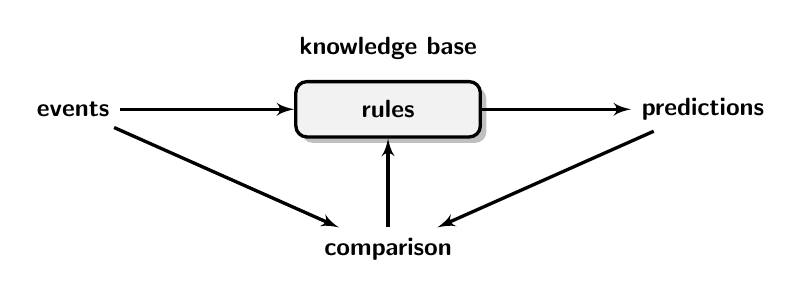
\begin{tikzpicture}[font=\small\sffamily\bfseries,very thick,node distance = 4cm]
\node [frame] (rul) {rules};
\node [above=5mm] (kb) {knowledge base};
\node [above=0cm, left of=rul] (eve) {events};
\node [above=0cm, right of=rul] (pred)  {predictions};
\node [below=1.5cm] (comp)  {comparison};
\path [line] (eve) -> (rul);
\path [line] (rul) -> (pred);
\path [line] (eve) -> (comp);
\path [line] (pred) -> (comp);
\path [line] (comp) -> (rul);
\end{tikzpicture}
\end{figure}

\emph{But}: Does this really work in the real world?

\paragraph{Diagnosis example:} toothache (using first order logic)
\begin{enumerate}[(1)]
\item $\forall p$ $symptom(p, toothache) \Rightarrow disease(p,cavity)$ \\
\indent $\leadsto$ rule is wrong: not all patients with toothache have cavities (gum disease, abscess, $\ldots$)
\item $\forall p$ $symptom(p, toothache) \Rightarrow$ \\
 $disease(p, cavity) \lor disease(p, gum disease) \lor disease(p, abscess) \lor \ldots$ \\
$\leadsto$ almost unlimited list of possible causes
\item diagnostic rule to causal rule \\
 $\forall p$ $disease(p, cavity) \Rightarrow symptom(p, toothache)$ \\
$\leadsto$ rule is wrong: not all cavities cause pain
\end{enumerate}
$\Rightarrow$ First order logic fails in many situations! Examples:
\begin{itemize}
	\item complete set of antecedents and consequences too large
	\item no complete theory for the domain
	\item incomplete observations
	\item stochastic environments
\end{itemize}
$\Rightarrow$ How can we deal with the fact that we are almost never 100\% sure
about our rules?
\paragraph{Degrees of belief}\mbox{}\\
\emph{Proposition} $H$: Patient $p$ has a cavity.
\[ \begin{array}{ll}
	P(H): H \rightarrow [0,1] 
	& \text{assignment of numbers} \\\\
	P(H) = 0
	& H \text{ is false} \\\\
	P(H) = 1
	& H \text{ is true} \\\\
	0 < P(H) < 1
	& \text{quantifies our degree of belief}
\end{array} \]
\emph{Formal treatment:} Assume $P(H)$ to obey the laws of probability theory
\begin{itemize}
  \itl ''probabilities''
  \itl but: no justification via repeated observations and stochastic outcome
\end{itemize}
(for detailed treatment, see \cite{Jaynes2003})
\\\\
\emph{Application to Betting agents:} (de Finetti, 1931)
\\
''If agent 1 expresses a set of degrees of belief that violate the
axioms of probability theory, then there is a combination of bets by
agent 2 that guarantees that agent 1 will lose money all the time.''
\\\\
Example: \textcite[p.474]{RussellNorvig2003}\slideref{betting agents}

% -----------------------------------------------------------------------------

\subsubsection{The Description of the World}
We start with a "sufficiently complete" set of random variables to describe the state of the world. 

\paragraph{Random variables and propositions}
\begin{description}
\item[Random variable:] a ''part'' of the world whose ''status'' is initially unknown  $\leadsto X, Y, \ldots$
\item[Domain of a random variable:] ''values'' the variable can take on 
\indent $\leadsto x, y, \ldots$
\end{description}
\paragraph{Examples}\mbox{}\\
Boolean variables:\\
\indent variable: $cavity$; domain: $\{true, false\}$ \\
\indent proposition: $cavity = true$\\
Discrete ordinal variables:\\
\indent variable: $weather$; domain: $\{sunny, rainy, cloudy, snow\}$ \\
\indent proposition: $weather = sunny$ \\
Continuous variables: \\
\indent variable: $temperature$; domain: $\mathbb{R}_0^+$ \\
\indent proposition: $temperature \in [290K, 291K]$
\paragraph{Atomic events}\mbox{}\\
Description of the ''world'': complete set of random variables \\
\indent e.g. $cavity, \; toothache, \; weather$
\\\\
Atomic event: complete specification of the state of the world \\
\indent e.g. $cavity = true \land toothache = false \land weather = sunny$
\begin{itemize}
  \itl atomic events are mutually exclusive
  \itl set of atomic events must be exhaustive
  \itl proposition $\corresponds$ disjunction of atomic events
\end{itemize}
\indent $cavity = true$ is equivalent to: \\
\indent $(cavity = true \land toothache = false \land weather = sunny) \lor$ \\
\indent $(cavity = true \land toothache = true \land weather = rainy) \lor \ldots$ 

\paragraph{Prior (unconditional) probabilities}\mbox{}\\ 
Specification of one's knowledge about the world - in the absence of any other information \\
\indent e.g. $P(cavity=true) = 0.1$ \\
\indent\indent $P(cavity=true,toothache=false,weather=snow) = 0.02$
\\\\
Complete specification of domain knowledge: table of degrees of belief for all atomic events \\
\indent e.g. $P(cavity,toothache,weather)$

\paragraph{Conditional probabilities}\mbox{}\\
Specification of one's knowledge about the world - given a set of observations (the ''evidence'').
\[ \begin{array}{l}
	P(cavity = true | toothache = true) = 0.8 \\
	P( \underbrace{cavity = false}_{ \text{proposition} }
	| \underbrace{ toothache = true}_{\substack{\text{observation /} \\
						\text{evidence}}}
	) = 0.2
\end{array} \]
$\Rightarrow$ conditional probability
\begin{equation}
	P( \underbrace{C}_{\text{variable}} | \underbrace{t}_{\text{value}} 
		) = \frac{ \overbrace{P(C,t)}^{\substack{\text{joint} \\
						\text{probability}}} }{
				P(t)}
\end{equation}
\begin{equation} \tag{product rule}
	P(C,t) = P(C|t) P(t)
\end{equation}
$P(C|t)$: degree of belief in $C$, given \underline{all} we know is $t$.

% -----------------------------------------------------------------------------

\subsubsection{Probabilistic Inference Using Joint Probabilities}
\emph{Knowledge base:} $P(x,y,\ldots)$ degrees of belief for all atomic events
\\\\
What is the probability of a proposition given a set of observations?
\[ \begin{array}{lll}
	\text{query variable:}
	& X & \leftarrow \text{ probability of values to be inferred}\\\\
	\text{evidence variable:}
	& E_j & \leftarrow \text{ observed variables} \\\\
	\text{unobserved variables:} 
	& Y_j & \text{"hidden" or "nuisance" variables}
\end{array} \]
\begin{equation}
	P(x | \vec{e}) = \underbrace{ \frac{P(x, \vec{e})}{P(\vec{e})} }_{
		\substack{\text{def. of cond.} \\ \text{probability}}}
		= \underbrace{ \alpha P(x, \vec{e}) }_{\text{normalization}}
		= \underbrace{ \alpha \sum\limits_{\vec{y}} 
			P(x, \vec{e}, \vec{y}) }_{\text{marginalization}}
\end{equation}
$\frac{1}{\alpha} = P(\vec{e}) = \sum\limits_{x,\vec{y}} P(x,\vec{e},\vec{y})$ involves a
sum over many different combinations of $x$ and $\vec{y}$ which can be
costly to evaluate. However, this does not have to be computed explicitly, because:
\begin{equation}		\tag{normalization of probabilities}
	\sum\limits_x P(x|\vec{e}) \eqexcl 1 
\end{equation}
This only uses knowledge $P(x,\vec{e},\vec{y}$) stored in the
knowledge-base, the \emph{product rule} and normalization
(for an example, see \cite[pp. 475]{RussellNorvig2003}). \slideref{marginalisation}

\paragraph{Note:} If we have the complete probability table for all atomic events, we have all the relevant information to do inference. 
\paragraph{Problem:} this ansatz does not scale! Assume $N$ binary random
variables:
\begin{itemize}
	\itl table of joint probabilities has $2^N$ entries
	\itl summation over approx. $2^N$ entries for inference\\ 
		$N = 100 \leadsto 2^N \approx 1.3 \cdot 10^{30}$ 
		$\leadsto$ additional assertion needed
\end{itemize}

% -----------------------------------------------------------------------------

\subsubsection{Conditional Independence}
\begin{center} \includegraphics[height=2cm]{section3_fig2} \end{center}
Cause and effect: $P(W|U) \rightarrow$ ''causal rule''\\
One cause and two effects: $P(W_1, W_2|U) = P(W_1|U) P(W_2|U)$\\\\
\emph{Example: }$P(\text{toothache}, \text{catch}| \text{cavity})
	= P(\text{toothache}|\text{cavity})
		P(\text{catch}|\text{cavity})$

\paragraph{Definition of conditional independence}\mbox{}\\
Two random variables $X$ and $Y$ are conditionally independent given $Z$ if:
\begin{equation}
	P(X,Y|Z) = P(X|Z) P(Y|Z)
\end{equation}
and we write $X\perp Y |Z$.\\\\
\emph{Note:} Conditional independence is \underline{not} independence:\\
\indent $\Rightarrow$ $X$ and $Y$ are typically \underline{not}
independent.
\\\\
\emph{Note:} Conditional independence assertions are an important step
towards efficient inference algorithms: they enable a 
\emph{decomposition} of the knowledge base. To illustrate this fact,
consider a set of binary random variables: $w_1, w_2, \ldots, w_{N-1},
U$.
\\\\
Assuming conditional independence of effects given the cause:
\begin{equation}
	\underbrace{
		\underbrace{ P(w_1, w_2, \ldots, w_{N-1}, U) }_{
		2^N-1 \text{ table entries}}
		= \underbrace{ P(U) \prod\limits_{i = 1}^{N-1} P(w_i|U) }_{
		1 + 2(N-1) = 2N-1 \text{ table entries}} }_{
			\text{probabilities sum to one}}
\end{equation}
$\Rightarrow$ greatly reduces computational burden to determine joint distribution from $O\big(2^N\big)$ to $O(N):$ this would solve the scaling problem!
\\\\
This approach is called ``naive Bayes'' can even be useful in
situations where conditional independence does \emph{not} strictly hold.
\begin{center} \includegraphics[height=2cm]{section3_fig3} \end{center}
$\Rightarrow$ use conditional probabilities as part of the model base
\subsubsection{Bayes' Theorem}
\paragraph{Common inference task:} Extract the causes underlying observations!
\[ \begin{array}{ll}
	\begin{array}{ll}
	\text{causal rule: } & P(W|U)P(U) \\\\
	\text{diagnostic rule: } & P(U|W)P(W) 
	\end{array}
	& \begin{array}{l}
	\includegraphics[height=1.5cm]{section3_fig4}
	\end{array}
\end{array} \]
\emph{Note:} In this graph, arrows do not represent causation but statistical dependency. 

\subsubsection*{Approach 1: causal knowledge base $\rightarrow$ diagnostic rule}
More generally, the joint probability $P(W,U)$ can be written as:
\begin{equation}\tag{Product rule}
	P(W|U)P(U) = P(W,U) = P(U|W)P(W)
\end{equation}
This can be used to infer $P(U|W)$ given $P(W|U)$ and $P(U)$ are known:
\begin{equation}\tag{Bayes' Theorem}
	P(U|W) = \frac{P(W|U)P(U)}{P(W)} = \alpha \; P(W|U)P(U)
\end{equation}
\underline{Comment 1:} Bayes' theorem holds for arbitrary random variables. ''Causes'' and ''effects'' were only used for illustration.

\subsubsection*{Approach 2: diagnostic knowledge base}
\emph{Advantage:} no calculations necessary to determine $P(U|W)$
\\\\
\underline{Comment 2:} Causal rules vs. diagnostic rules
\[ \left. \begin{array}{ll}
	\text{M:} & \text{meningitis} \\
	\text{S:} & \text{stiff neck}
\end{array} \right \} P(M|S) \]
Diagnostic knowledge base: $P(M|S)$ is directly stored. No computation
\\\\
causal knowledge base: $P(M|S) = \underbrace{ \alpha P(S|M) P(M) }_{
	\substack{\text{Bayes'} \\ \text{theorem}}}$\\
\indent $\rightarrow$ constructed from hospital records
\\\\
\emph{Problem:} Consider a sudden epidemic of meningitis: $P(M) \uparrow$ \\
\indent $\leadsto$ diagnostic knowledge base $p(M|S)$ cannot be updated easily

% -----------------------------------------------------------------------------

\newpage					% NEWPAGE for visual reasons
\subsection{Bayesian Networks}
\[ \text{Bayesian network} \left \{ \begin{array}{l}
	\text{- representation of the joint probability distribution} \\
	\text{- encoding of a collection of conditional independence statements}
\end{array} \right. \]
{\bf \underline{D}irected \underline{A}cyclic \underline{G}raphs (DAG)}
\begin{itemize}
	\item set of random variables 
		\begin{itemize}
			\itl nodes of the graph
		\end{itemize}
	\item direct influence between variables (e.g. causal relationships)
	\begin{itemize}
		\itl directed links between nodes
	\end{itemize}
	\item nodes are annotated with conditional probability distributions
		\[ P(x_i| parents(x_i)) \]
\end{itemize}
For details, see \textcite[ch. 14: Probabilistic Reasoning]{RussellNorvig2003}. 

\paragraph{Example:} Burglary detection in california: What is the probability of a burglary given that John and/or Mary call? 
\begin{center} \includegraphics[width=10cm]{section3_fig5} \end{center}
\begin{equation}
	P(J,M,A,B,E) = P(J|A)P(M|A)P(A|B,E)P(B)P(E)
\end{equation}
\emph{Bayesian network:}
\[ \begin{array}{lcl}
	\substack{\text{directed acyclic graph} \\ \text{annotated nodes}}
	& \longleftrightarrow &
	P(x_1, \ldots, x_N) = \prod\limits_{i=1}^n P(x_i|\mathrm{parents}(x_i))
\end{array} \]

\paragraph{Inference:} What is the probability of burglary - given that both Mary and John call?
\begin{center} \includegraphics[width=8cm]{section3_fig6} \end{center}
To determine this probability, we need to marginalize over the two 
nuisance variables \texttt{Alarm} ($a$) and \texttt{Earthquake} ($e$):
\begin{equation}
	\begin{array}{lll}
	P(B|J=true, M=true) 
	& = & \underbrace{ \alpha P(B, J=true, M=true) }_{
		\substack{ \text{normalization} \\ \text{c.f. section 3.1.3}}} \\\\
	& = & \underbrace{ \alpha \sum\limits_{a,e} P(B, e, a, 
				J=true, M=true) }_{
		\text{marginalization}} \\\\
	& = & \alpha P(B) \sum\limits_e P(e) \sum\limits_a P(a|B,e) \\
	&& \cdot P(J=true|a) P(M=true|a) \\\\
	& = & \alpha \cdot \left \{ \begin{array}{ll}
			0.00059224 & \text{for } B=true \\\\
			0.0014919 & \text{for } B=false
		\end{array} \right.
	\end{array}
\end{equation}
Choose $\alpha$, such that sum is 1:
\begin{equation}
	P(B|J=true, M=true) = \left \{ \begin{array}{clc}
		0.284 & \text{for } B=true & 0.001 \\\\
		\underbrace{0.716}_{\substack{\text{evidence changed} \\
					\text{our assessment}}}
			& \text{for } B=false 
			& \underbrace{0.999}_{\text{Prior } P(B)}
	\end{array} \right.
\end{equation}
\textbf{Question:} How can we efficiently implement inference in larger and more complex Bayesian networks?

% -----------------------------------------------------------------------------

\subsubsection{Directed Acyclic Graphs}
Directed Acyclic Graphs (DAG's) provide useful graph structures to
represent probabilistic knowlege bases (cf.\ feedforward neural networks).
\begin{equation*}
\begin{array}{ll}
	\raisebox{-10mm}{\includegraphics[width=4cm]{section3_fig7}}
	& \begin{array}{l}
		\text{Graph } G = (V, K) \\\\
		\begin{array}{ll}
			V & \rightarrow \text{ set of nodes} \\\\
			K & \rightarrow \text{ set of links}
		\end{array}
	\end{array}
\end{array}
\end{equation*}
\begin{description}
\item[path:]sequence $\big\{ x_i \big\}, i=1, \ldots, n$ of different nodes $x_i \in V$, such that $\big( x_i, x_{i+1} \big) \in K$ 
\item[cycle:] path with property  $x_1 = x_{n+1}$ 
\item[parents and children] of nodes:
\begin{center} \includegraphics[width=4cm]{section3_fig8} \end{center}
\end{description}
\textbf{DAGs and distributions:} Graphical models provide a link
between graph structures and probability distributions. This link
allows to use results from graph-theory to implement efficient
inference algorithms.\\\\
\textbf{Note:} Every DAG corresponds to a factorization of a joint PDF!
\begin{equation}
	\begin{array}{ccc}
	P(x_1, \ldots, x_n) & = & \prod\limits_{i=1}^n P(x_i|parents(x_i)) \\\\
	\text{''causal flow''} & \longleftrightarrow 
		& \text{well ordered nodes} \\\\
	\substack{\text{useful for construction} \\ \text{of compact networks}}
	&& \substack{\text{index of a node } x_i \text{ should always} \\
		\text{be larger than all indices of its parents}}
	\end{array}
\end{equation}

\paragraph{Topological sorting:} Naming nodes according to causal
flow. Application of \algfont{algorithm~\ref{alg:topological-sorting}} results
in a well ordered sorting of nodes corresponding to a factorization of
the joint pdf.
\begin{algorithm}
  \DontPrintSemicolon
  DAG with nodes without indices\;
  $i = 1$\;
  \While{nodes are left within DAG}{
    choose node without parents\;
    set index of node to $i$\;
    delete node and all its links from DAG\;
    $i\leftarrow i+1$\;
  }
\caption{Topological sorting}
\label{alg:topological-sorting}
\end{algorithm}

\paragraph{Comment:} conditional independence $\Rightarrow$ encoded by graph structure
\begin{enumerate}[(1)]
\item A node is conditionally independent of its non-descendants - given its parents
\item A node is conditionally independent of all other nodes in the network - given its parents, children and children's parents (Markov blanket)
\end{enumerate}
for further details, see \textcite[ch.14, Fig 14.4]{RussellNorvig2003}.\slideref{Markov Blanket}

\paragraph{Properties of DAGs}
\begin{itemize}
	\item efficient representation of knowledge about (causal) relationships 
		between variables
	\item \emph{topology}: qualitative relationships (causality, conditional 
		independence)
	\item \emph{annotation}: quantitative information (probability tables of pdfs)
	\item straightforward to construct
\end{itemize}
\emph{Problem}: DAGs do not provide an efficient representation for
inference (one of the central aims of using graphical models). Such a
respresentation, however, can be constructed on the basis of the
corresponding decomposable undirected graph.

% -----------------------------------------------------------------------------

\subsubsection{Decomposable Undirected Graphs}
\[\begin{array}{ll}
	\includegraphics[width=4cm]{section3_fig9}
	& \substack{\text{undirected graph:} \\ 
		\text{graph with undirected links}}
\end{array} \]
\paragraph{Separator}\mbox{}\\
Consider $A, B, C \subset V$ (not necessarily disjoint)\\\\
$\Rightarrow C$ separates $A$ and $B$, if every path from an arbitrary node from $A (x_1 \in A)$ to an arbitrary node from $B (x_n \in B)$ passes through at least one node from $C$.
\[ \begin{array}{ll}
	\includegraphics[width=4.5cm]{section3_fig10}
	& C \text{ separates } A \text{ and } B
      \end{array} \]
\textbf{Complete graph:} a graph in which every pair of nodes is connected by an edge.

\paragraph{Proper decomposition of $G = (V,K)$}\mbox{}\\
Consider $V = A \cup B \cup C$ with $A,B,C$ non-empty and disjoint
\\\\
$\Rightarrow A,B,C$ is a proper decomposition of $G$ if:
\begin{itemize}
	\itl $C$ separates $A$ and $B$
	\itl $C$ is complete 
\end{itemize}
\[ \begin{array}{ll}
	\includegraphics[width=4.5cm]{section3_fig11}
	& \substack{C \text{ separates } A \text{ and } B\\
		A,B,C \text{ is proper decomposition}}
\end{array} \]
\paragraph{Decomposable graph}
\begin{itemize}
	\itl complete graph \underline{or}
	\itl there exists a proper decomposition $A,B,C$ such that both 
		subgraphs $G_{A \cup C}$ and $G_{B \cup C}$ are both proper 
		decomposable
\end{itemize}
\[ \begin{array}{ccc}
	\includegraphics[width=4cm]{section3_fig12}
	& \includegraphics[width=4cm]{section3_fig13}
	& \includegraphics[width=4cm]{section3_fig14} \\\\
	\substack{ \text{not decomposable} \\
		\text{(no separator of } A \cup C \text{ is complete} \\
		\text{nor is } A \cup C \text{ complete)}}
	& \text{decomposable}
	& \text{decomposable or complete}
\end{array} \]
$\Rightarrow$ decomposition into \underline{maximally complete subgraphs (''cliques'')} separated by ''separators''

\begin{center} \includegraphics[width=12cm]{section3_fig15} \end{center}

\paragraph{Decomposable graphs and distributions: }
Decomposable graphs provide a useful factorization of the joint
distribution allowing to efficiently calculate marginals ($\rightarrow$
inference, see 3.2.4/5).


\begin{enumerate}[(1)]
\item $A$ is conditionally independent of $B$ given $C$ \\
$\Leftrightarrow A,B,C$ is a proper decomposition of $G$
\item $\begin{array}{ll}
	P(\vec{x}) = \frac{ \prod\limits_{\text{cliques }C} P_C(\vec{x}_C) }{
			\prod\limits_{\text{separators }S} P_S(\vec{x}_S)}
	& \substack{\text{decomposable graph} \\
		\longleftrightarrow \text{ factorization into} \\
			\text{marginal distributions}}
\end{array} $
\end{enumerate}
\textbf{Note:} The cliques (separators) are annotated by the marginal
probability distributions over the corresponding clique (separator)
variables.
\begin{center} \includegraphics[width=4cm]{section3_fig16} \end{center}
\begin{equation}\label{eq:marginalRepresentation}
	P(x_1, \ldots, x_6) = \frac{ \overbrace{ P(x_1, x_2, x_3) 
					P(x_2, x_3, x_4) P(x_4, x_5, x_6)}^{
						\text{cliques}}}{
				\underbrace{P(x_2, x_3)P(x_4)}_{
					\text{separators}}}
\end{equation}
This is a valid distribution, because:
\begin{eqnarray*}
\frac{ \prod_{C \in \mathcal{C}} P_C(\vec{x}_C) }{
			\prod_{S \in \mathcal{S}} P_S(\vec{x}_S)}
& = & \frac{ P(x_1, x_2, x_3) P(x_2, x_3, x_4) P(x_4, x_5, x_6)}{P(x_2, x_3)P(x_4)} \\
 & = &  P(x_1|x_2,x_3) P(x_2,x_3|x_4) P(x_4,x_5,x_6) \\
  & = & P(x_1|x_2,x_3) P(x_2|x_3,x_4) P(x_3) P(x_4|x_5,x_6) P(x_5|x_6) P(x_6) \\
  & = & \prod\limits_{i=1}^6 P(x_i|x_{i+1}, \ldots, x_6) \\
  & = & P(x_1, x_2, \ldots, x_6)
\end{eqnarray*}
\begin{center} \includegraphics[width=4cm]{section3_fig17} \end{center}
\begin{itemize}
	\itr every decomposable undirected graph represents a valid probability 
		distribution
	\itr full marginalization: complexity $\mathcal{O}(2^n)$, $n$: cardinality of the 
		largest clique
\end{itemize}
\textbf{Note:} The general factorization into potentials is not unique!
\begin{equation}
	\begin{array}{ll}
		P(\vec{x}) \sim \frac{\prod\limits_{\text{cliques }C} 
					\psi_C (\vec{x}_C)}{
				\prod\limits_{\text{separators }S} 
					\psi_S (\vec{x}_S)} 

	\end{array}
\end{equation}
Shifting factors between terms in the numerator and denominator
results in the same value. This will become important for inference.
% -----------------------------------------------------------------------------

\newpage 						% --- for visual reasons
\subsubsection{Marginal Distributions and Inference on Decomposable Graphs}
The following example illustrates how the representation of the joint
distribution in terms of potential functions can be transformed into a
representation based on the marginal probabilities over the
corresponding cliques
(cmp.~\cite[p.~84]{CowellEtAl2003}). Consider the distribution
over 3 random variables $X,Y,Z$ described by the following graph:

\begin{center} \includegraphics[width=8cm]{section3_fig18} \end{center}
\begin{equation}\label{eq:potentialRepresentation}
	P(x, y, z) = \alpha \frac{f(x, y) g(y, z)}{h(y)}
\end{equation}

\paragraph{Goal:} calculate factorization into marginals
\\
\emph{Starting point:} factorization into potentials (here: $f,g,h$) often straightforward to construct, e.g.
\begin{equation}
  P(x,y,z) = \frac{ \overbrace{P(x|y)}^{\corresponds f(x,y)}
    \overbrace{P(y|z)P(z)}^{\corresponds g(y,z)}}{
    \underbrace{1}_{\corresponds h(y)}}
\end{equation}
\begin{center} 
  \includegraphics[width=6cm]{section3_fig19} 
\end{center}
Furthermore, inference problems lead to a potential-based representation for
the conditional probability distributions. \\\\
Consider, e.g.\ inference given observed evidence: $Z=z$
\begin{equation}
  P(x,y|z) = \frac{P(x,y,z)}{P(z)} = \alpha' P(x,y,z)
  = \alpha \frac{f(x,y) g(y,z)}{h(y)}
\end{equation}
indicator functions:
\begin{equation}
  E(z) = \left \{ \begin{array}{ll}
      1, & \text{if } Z = z\\
      0, & \text{else}
    \end{array} \right.
\end{equation}
\begin{equation}
  \underbrace{P(x,y|z)}_{P^{(z)}(X,Y,Z)} = 
  \alpha \frac{f(x,y)
    \overbrace{g(y,z)E(z)}^{\substack{
        \text{new clique} \\
        \text{- potential -}\\
        \text{after observing} \\
        \text{the evidence}}
    }}{h(y)}
\end{equation}
\begin{equation}
  \Rightarrow P^{(z)}(x, y, z) = \alpha
  \frac{f(x,y)g^{(z)}(y,z)}{
    h(y)}
\end{equation}

\paragraph{Calculation through message passing:}The representation of
the joint probability in terms of clique potentials
(eq.~\ref{eq:potentialRepresentation}) can be transformed into a
representation in terms of the marginal probabilities over the
corresponding cliques (cmp. \ref{eq:marginalRepresentation}) which is
useful e.g.\ to infer conditional probabilities.
\begin{enumerate}[(1)]
\item The marginal distribution of $P(x,y)$ can be calculated from the
  clique-representation
 \begin{equation}
	\begin{array}{ll}
		P(x,y) 
		& = \sum\limits_{z} P(x,y,z) \\\\
		& = \alpha \frac{f(x,y)}{h(y)} \underbrace{
			\sum\limits_{z} g(y,z)}_{\eqexcl h^*(y)} \\\\
		& = \alpha \underbrace{ f(x,y) \frac{h^*(y)}{h(y)} }_{
			\eqexcl f^*(x,y)}
	\end{array}
\end{equation}
This means that $f^*(x,y) \sim P(x,y)$ and can be calculated from the
potential $f(x,y)$ by passing to it a ``message'' containing the \emph{update ratio}
$\frac{h^*(y)}{h(y)}$ calculated from the clique potential $g(y,z)$
and the separator potential $h(y)$. This way we get a representation
of the joint distribution in terms of the updated (*) potentials: 
\begin{equation}
	\begin{array}{ll}
		P(x,y,z) 
		& = \alpha f(x,y) \frac{1}{h(y)} \frac{h^*(y)}{h^*(y)} 
			g(y,z)\\\\
		& = \alpha f^*(x,y) \frac{1}{h^*(y)}g(y,z)\\\\
	\end{array}
\end{equation}
\item The marginal distribution of clique $P(y,z)$ can be calculated in the same way
\begin{equation}
	\begin{array}{ll}
		P(y,z) 
		& = \sum\limits_x P(x,y,z) \\\\
		& = \alpha \underbrace{\bigg(\sum\limits_x f^*(x,y) \bigg)}_{
				\eqexcl h^+(y)} \frac{1}{h^*(y)} g(y,z)\\\\
		& = \alpha \underbrace{\frac{h^+(y)}{h^*(y)} g(y,z)}_{
				 \eqexcl g^+(y,z)}
	\end{array}
\end{equation}
Yielding the updated potential $g^+(y,z) \sim P(y,z)$ and the joint representation in terms of both updated potentials: 
\begin{equation}
	\begin{array}{ll}
		P(x,y,z) 
		& = \alpha f^*(x,y) \frac{h^+(y)}{h^+(y)}
			\frac{1}{h^*(y)} g(y,z)  \\\\
		& = \alpha f^*(x,y) \frac{1}{h^+(y)} g^+(y,z)
	\end{array}
\end{equation}
\item Marginal distribution of the separator $P(y)$
 \begin{equation}
	\begin{array}{ll}
		P(y) 
		& = \sum\limits_x P(x,y) \\\\
		& = \alpha \sum\limits_x f^*(x,y)\\\\
		& = \alpha h^+(y) \\\\
		& \Rightarrow h^+(y) \sim P(y)
	\end{array}
\end{equation}
\item Joint distribution: collecting terms shows that the updated representation is, indeed, based on the clique-marginal distributions. 
\begin{equation}
	\begin{array}{ll}
		P(x,y,z) 
		& = \alpha \frac{P(x,y)}{\alpha}
			\frac{\alpha}{P(y)} 
			\frac{P(y,z)}{\alpha}\\\\
		& = \frac{P(x,y)P(y,z)}{P(y)}
	\end{array}
\end{equation}
\end{enumerate}
\slideref{message passing\\ \& local\\ computation} 
\[ \text{message passing} \left \{ \begin{array}{l}
	\text{for calculating prior marginals} \\\\
	\text{for calculating posteriors marginals (after observation of 
		evidence)}
\end{array} \right. \]

% -----------------------------------------------------------------------------

\subsubsection{Belief Propagation and the Junction Tree Algorithm}
\paragraph{Overview}
\begin{enumerate}[(1)]
\item  \emph{definition of state variables \& construction of the Bayesian network:}
\begin{enumerate}[-a-]
	\item directed acyclic graph (expert analysis, causal relationship)
	\item topological sorting
	\item annotation with conditional probabilities (expert
          knowledge, extraction of fractions from database, ... inductive learning?)
        \end{enumerate}

\item \emph{ construction of the inference engine}
\[ \begin{array}{ccl}
	\text{-a-} & \text{directed acyclic graph} & \leftarrow \text{ annotated with 
					conditional pdfs} \\
	& \downarrow \\
	\text{-b-} & \text{moral graph}\\
	& \downarrow \\
	\text{-c-} 
& \text{undirected decomposable graphs} & \leftarrow \text{ annotated with
					clique and separator potentials}\\
	& \downarrow \\
	\text{-d-} & \text{junction tree} & \leftarrow \text{ final data structure for 
					message passing}
\end{array} \]

\item \emph{inference:} processing the evidence
\begin{enumerate}[-a-]	
  \item initialization
  \item modification of clique potentials by observed evidence (not when 
  just calculating prior)
  \item message passing (''belief propagation'')
  \item final marginalization within relevant clique
\end{enumerate}
\end{enumerate}


\paragraph{Details ad (2) -- Construction of the inference engine}\label{sec:details}
\begin{enumerate}[-a-]
\item directed acyclic graph
\item construction of the related moral graph \slideref{DAG\\$\downarrow$\\moral\\graph}
  \begin{itemize}
    \itr connect all parents of a node with undirected links (for 
    all nodes)
    \itr replace all directed links with undirected links 
  \end{itemize}
  \item construction of a related undirected decomposable graph\slideref{undirected\\ decompos.\\ graph} 
  \begin{itemize}
    \itr add undirected links such that all cycles of length four and
    larger contain a chord \itr chordal graph is always decomposable\footnote{for a proof, see Cowell et. al. theorem 4.4} \slideref{triangulation algorithm}
    \itr chordal graph is not unique 
    \itr construction of a chordal graph with cliques of minimal size is NP hard 
  \end{itemize}
  \item construction of a related junction tree
  \begin{itemize}
    \itr \emph{nodes of the junction tree}:\\
    maximal cliques of the decomposable graph
    \itr \emph{links of the junction tree}:\\
    connect neighboring maximal cliques annotated by the corresponding separators \slideref{construction of the junction tree}
    \itr after the first loop, the running intersection
    property holds, i.e. for all $1 < j \leq k$ 
    there exists one $i < j$, such that $C_j \cap
    \big( C_1 \cup \ldots \cup C_{i-1} \big) 
    \subseteq C_i$
    \itr but: nodes may not only be cliques, but could be 
    other complete subgraphs
    \itr second loop estimates those nodes
  \end{itemize}
\end{enumerate}

\paragraph{Details ad (3) -- Inference: processing of the evidence}
\label{sec:infer-proc-evid}
\begin{enumerate}[-a-]
  \item initialization of the clique and separator potentials   \slideref{initialization of cliques and separators}
  \begin{equation}	
    P(\vec{x}) = \prod\limits_k P(x_k|parents(x_k)) 
    \leftarrow \text{ from annotated DAG}
  \end{equation}
   \begin{algorithm}
     \DontPrintSemicolon
     Set all clique and separator potentials to $\psi_{C,S}(\vec{x}_{C,S}) = 1$\;
     \For{all nodes $x_k$ of the DAG}{
       Find a node of the junction tree which contains $x_k$ and its parents\; 
       Multiply corresponding clique potential with $P(x_k|parents(x_k))$}
     \caption{Initialization of clique potentials}
   \end{algorithm}

\item modification of clique potentials by observed evidence 
  \begin{itemize}
  \itr for given observations $\vec{X}_e = \vec{x}_e$, set clique potentials to:
  \begin{equation}
    P(\vec{x}/\vec{x}_e|\vec{x}_e) =
    \alpha P(\vec{x}) 
    \underbrace{\prod\limits_{j \in e}}_{
      \substack{\text{multiplied to} \\
        \text{the proposed} \\
        \text{clique potential}}}
    \underbrace{E(x_j)}_{\substack{\text{indicator
          functions}\\
        E(x_j) = \left\{ \begin{array}{ll}
            1, & \text{ if } X_j = x_j\\\\
            0, & \text{ else}
          \end{array} \right.}}
  \end{equation}
  \end{itemize}


  \item calculation of marginal probabilities: belief propagation
    \begin{itemize}
      \itr ''collect evidence'' (1st pass): choose a root node from the junction tree, broadcast ``request'' \& collect
      \[ \begin{array}{ll}
        \includegraphics[width=4cm]{section3_fig20} 
        & \text{broadcast of request} \\\\
        \includegraphics[width=4cm]{section3_fig21} 
      & \substack{ \text{transmission of 
          messages (and} \\
        \text{modification of 
          potentials)}}
    \end{array} \]
    \itr ''distribute evidence'' (2nd pass) 
    \[ \begin{array}{ll}
      \includegraphics[width=4cm]{section3_fig22} 
      & \substack{ \text{transmission of 
          messages (and} \\
        \text{modification of 
          potentials)}}
    \end{array} \]
    \itR \begin{equation}
      \left. \begin{array}{l}
          P(\vec{x}) = \frac{\prod\limits_{\text{cliques }
              C} P_C(\vec{x}_C)}{\prod\limits_{
              \text{separators }S} P_S(
            \vec{x}_S)}
        \end{array} \right \} \text{marginal
        distributions}
    \end{equation}
  \end{itemize}
\item marginalization within relevant clique

\end{enumerate}

% -----------------------------------------------------------------------------

\newpage 						% --- for visual reasons
\subsection{Bayesian Inference and Neural Networks}

% -----------------------------------------------------------------------------
\subsubsection{Generative Models}
observations: $\vec{z}^{(\alpha)} = \big( \underbrace{ \vec{x}^{(\alpha)} }_{
	\substack{ \text{independent} \\ \text{variable} }}, 
	\underbrace{ \vec{y}_T^{(\alpha)} }_{ \substack{ \text{associated} \\
		\text{variable}} } \big), \alpha = 1, \ldots, p$
\\\\
true distribution:
\begin{equation}
	p_{(\vec{z})} = \underbrace{p_{(\vec{y} | \vec{x})}}_{
		\substack{ \text{conditional} \\ \text{probability} }}
	p_{(\vec{x})}
\end{equation}
\emph{previous approach:}
\begin{itemize}
	\itl construct a parametrized class $y_{(\vec{x};\vec{w})}$ of 
		(deterministic) predictors
	\itl inference is based on a single selected (optimal) predictor 
		$y_{(\vec{x}; \vec{w}^*)}$
\end{itemize}
\emph{generative model approach:}
\begin{itemize}
	\itl construct a parametrized class $p_{(\vec{y}|\vec{x};\vec{w})}$
		of (conditional) densities
	\itl inference is based on good ''generative models''
\end{itemize}
\begin{center}
$\underbrace{ \fbox{ \text{''generative'' model of a data source} } 
	}_{ \substack{
		\text{description of the data} \\
		\text{generation process} }}
\longrightarrow \fbox{ \text{observations} }$
\end{center}
\emph{Comment:}
\begin{itemize}
	\item[] models $p_{(\vec{z};\vec{w})}$ for unconditional densities
		$\leadsto$ unsupervised learning 
		\\ (e.g. ICA, mixture models)
	\item[] models $p_{(\vec{y}|\vec{x};\vec{w})}$ for conditional 
		densities $\leadsto$ supervised learning
\end{itemize}
\paragraph{Example I:} Generative model for simple regression
\begin{center}
\includegraphics[width=6cm]{section3_fig23} 
\end{center}
\emph{Description of the data generation process:}
\begin{equation}
  y_{(\vec{x})} = 
  \underbrace{ \widehat{y}_{(\vec{x};\vec{w})} }_{
    \substack{ 	\text{model of a deterministic} \\
      \text{relationship}}}
    + \underbrace{\widehat{\eta}}_{
      \substack{\text{model of the noise} \\
       \text{here: additive noise}}}
\end{equation}
The deterministic relationship is typically modeled with a
parametrized function e.g.\ a polynomial or a neural network. Noise is
often assumed to be additive but could also be multiplicative. Here, we model
noise with a parametrized distribution 
$\widehat{p}_{(\widehat{\eta}; \vec{\sigma})}$. 

\paragraph{Common noise models}\mbox{}\\
Additive Gaussian noise:
\begin{equation}
	\widehat{p}_{(y|\vec{x};\vec{w})} 
	= \frac{1}{\sqrt{2 \pi} \sigma} \exp \Bigg\{
		-\frac{ \big( y - \widehat{y}_{(\vec{x};\vec{w})} \big)^2 }{
			2 \sigma^2} \Bigg\}
\end{equation}
Additive Minkowski noise:
\begin{equation}
	\widehat{p}_{(y|\vec{x};\vec{w})} 
	= \frac{d \beta^{\frac{1}{d}}}{2 
		\underbrace{ \Gamma_{(\frac{1}{d})} }_{
			\substack{ 	\text{Gamma} \\
					\text{function} }
			} }
		\exp \Big\{ -\beta \big| y - \widehat{y}_{(\vec{x};\vec{w})}
			\big|^d \Big\}
\end{equation}
\indent $d = 1$: exponential function
\begin{equation}
	\widehat{p}_{(y|\vec{x};\vec{w})}
	= \frac{\beta}{2} \exp \Big\{ -\beta \big| y - 
		\widehat{y}_{(\vec{x};\vec{w})}	\big|^d \Big\}
\end{equation}
\indent $d = 2$: Gaussian distribution
\begin{center}
\includegraphics[width=12cm]{section3_fig24} 
\end{center}
\paragraph{Example II:} Classification for $c$ classes $C_k, k = 1, \ldots, c$
\\\\
\emph{Description of the data generation process:}
\begin{equation}
	p_{(C_k|\vec{x})} = y_{k(\vec{x})}
\end{equation}
\begin{itemize}
	\itl label noise (e.g. overlapping classes)
\end{itemize}
\emph{Model:}
\begin{equation}
	\widehat{p}_{(C_k|\vec{x};\vec{w})} = y_{k(\vec{x};\vec{w})}
\end{equation}
\begin{itemize}
	\itl general parametrized model (e.g. neural network: section 1.4.7)
\end{itemize}

% -----------------------------------------------------------------------------

\subsubsection{Bayesian Model Selection}
\emph{Reasoning under uncertainty} (cf.\ section 3.1.4)
\[ \begin{array}{lcl}
	\text{causal rules:}
	& \includegraphics[width=5cm]{section3_fig25} 
	& \text{''generative model''} \\\\
	\text{diagnostic rules:}
	& \includegraphics[width=5cm]{section3_fig26}
	& \substack{ 	\text{''model evaluation''} \\
			\leadsto \text{ evaluating the evidence}} \\\\
	& \includegraphics[width=5cm]{section3_fig27}
\end{array} \]
\emph{Degree of belief in a given model}
\begin{itemize}
	\itl set $\{ M_i \}$ of disjunct models (hypotheses) $M_i$
	\itl a random observed event $E$ (evidence)
\end{itemize}
\emph{Bayes rule:}
\begin{equation}
	\underbrace{ P_{(M_i|E)} }_{\substack{\text{posterior}}}
	= \frac{ \overbrace{ P_{(E|M_i)} }^{ \substack{ \text{likelihood}}}
	\overbrace{ P_{(M_i)} }^{\substack{\text{prior}}}
	}{ \underbrace{ P_{(E)} }_{\substack{\text{normalization constant}\\
		\text{(''evidence'')}}} }
\end{equation}
\textbf{Likelihood} $P_{(E|M_i)}$: probability of observing the evidence $E$, given that model $M_i$ is true $\Leftarrow \fbox{\text{''generative model''}}$
\\\\
\textbf{Prior} $P_{(M_i)}$: our degree of belief in $M_i$, before $E$ has been observed
\\\\
Initialization of prior beliefs $\rightarrow$ maximum entropy methods
\begin{equation}
	\begin{array}{lc}
	-\sum\limits_i P_{(M_i)} \ln P_{(M_i)} \eqexcl \max
	& \substack{ 	\text{find least informative} \\
			\text{prior beliefs}}
	\end{array}
\end{equation}
\emph{Constraints:}
\begin{equation}
	\begin{array}{lc}
	\sum\limits_i P_{(M_i)} = 1 
	& 
	\substack{	\text{normalization of} \\
			\text{probabilities}} \\\\
	\substack{ 	\text{information about (e.g.)} \\
			\text{moments of meanwhile} \\
			\text{quantities} }
	& \substack{ 	\text{formal description of} \\
			\text{prior knowledge}}
	\end{array}
\end{equation}
\begin{itemize}
	\itR solution using Lagrange multipliers
	\itR if no prior knowledge exists:
	\begin{equation}
		P_{(M_i)} = \mathrm{const.}
	\end{equation}
	\begin{equation}
		P_{(M_i|E)} \sim P_{(E|M_i)}
	\end{equation}
\end{itemize}

% -----------------------------------------------------------------------------

\subsubsection{Bayesian Prediction}
Predictions regarding future data $e$ will depend on both the observed
evidence $E$ and the model $M$ used. The \emph{predictive distribution} combines predictions from multiple models and weights them, depending on how probable these models are given the data observed so far ($\rightarrow$ posterior distribution of models/parameters given observed evidence).\\\\
\emph{The predictive distribution:}
\begin{equation}
	\substack{ 	\text{observations } E}
	\xrightarrow{ \substack{	\text{fundamental problem} \\
					\text{of prediction}} }
	\substack{	\text{degree of belief } P_{(e|E)} \\
			\text{into a new event } e}
\end{equation}
\begin{equation}
	\begin{array}{llc}
	P_{(e|E)} 
	& = \sum\limits_i P_{(e, M_i|E)}
	& \substack{ \text{marginalization} } \\\\
	& = \sum\limits_i P_{(e|M_i, E)} P_{(M_i|E)}
	& \substack{ \text{def. of conditional probability} } \\\\
	& \eqexcl \sum\limits_i P_{(e|M_i)} P_{(M_i|E)}
	& \substack{ \text{conditional independence assumption} }
	\end{array}
\end{equation}
\begin{itemize}
  \itr only ok if model fully describes data generation
  \itr only approximately fulfilled in reality
  \itR committee-ansatz (Bayesian committee)
\end{itemize}

\paragraph{Prediction and evaluation of distribution:}
After selection of a ''predicted attribute'' (see below) one can make a
decision based on $P_{(e|E)}$. In many cases it might not be
optimal to simply choose the maximally probable value because there are
additional constraints to consider, e.g. estimated loss if a
prediction error occurs. 
\\\\
\emph{Loss function:}
\begin{equation}
	C_{( \underbrace{ e }_{ \substack{	\text{true} \\
						\text{value}} }
		, \underbrace{ \widehat{e} }_{ \substack{
			\text{predicted} \\
			\text{value} \\
			\text{(based on } \\
			P_{(e|E)} \text{)}}} )}
\end{equation}
Instead of choosing the maximally probable value, it is therefore a common strategy to minimize the expected loss
\begin{equation}
	\widehat{e} = \argmin\limits_{\tilde{e}}
		\int d e C_{(e, \tilde{e})} P_{(e|E)}
\end{equation}

% -----------------------------------------------------------------------------

\subsubsection{Application: MLPs with weight decay}
For some simple models such as linear regression, the posterior
parameter distribution and the predictive distribution can be analysed
in closed form ($\leadsto$ Bayesian linear regression). For more
flexible models, exact analytical treatment is not available such that
evaluation of the predictive distribution requires approximation
techniques (e.g.\ sampling, variational inference). 

Here, we discuss another alternative, the \emph{Laplace
  approximation}, which (a) approximates the true posterior parameter
distribution with a Gaussian centered on a MAP estimate and (b)
assumes the network function to be approximately linear around this
point.

To determine the posterior parameter distribution from a given set of
training data we will (a) formulate the likelihood function for a
given class of generative models, (b) determine the maximum entropy
prior distribution, and (c) use Bayes rule to combine them.
\\

\emph{training data:} $\Big\{ \big( \vec{x}^{(\alpha)}, y_T^{(\alpha)} \big)
	\Big\}, \alpha = 1, \ldots, p$ \\

\emph{abbreviations:} $X = \Big\{ \vec{x}^{(\alpha)} \Big\}, 
	Y = \Big\{ \vec{y}_T^{(\alpha)} \Big\}$


\paragraph{(a) Construction of the model class}
$\rightarrow$ likelihood of the data 
\begin{equation}
	P_{\big( y_T^{(\alpha)}| \vec{x}^{(\alpha)}; \vec{w} \big)}
	\sim \exp \Big\{ -\beta \underbrace{ 
		e_{\big( y_T^{(\alpha)}, \vec{x}^{(\alpha)}; 
		\vec{w}\big)}^T }_{ \substack{
			\text{almost always possible,} \\
			\text{because } P \text{ positive}}}
	\Big\}
\end{equation}
\begin{equation}
	\begin{array}{ll}
	P_{(Y|\vec{x};\vec{w})}
	& \sim \prod\limits_{\alpha} \exp \Big\{ -\beta 
		e_{\big( y_T^{(\alpha)}, \vec{x}^{(\alpha)}; \vec{w}\big)}^T
		\Big\} \\\\
	& \sim \exp \Big\{ -\beta \sum\limits_{\alpha} 
		e_{\big( y_T^{(\alpha)}, \vec{x}^{(\alpha)}; \vec{w}\big)}^T
		\Big\} \\\\
	& \sim \exp \left\{-\beta E^T \right\}
	\end{array}
\label{eq:likelihoodData}
\end{equation}
where $E^T:=E_{(Y, \mathrm{x}; \vec{w})}$ denotes the training
error. This shows a direct relation between minimisation of the
mean squared error and Maximum likelihood estimation under the
assumption of additive Gaussian noise:
\begin{equation}
	P_{(Y| \vec{x};\vec{w})} = 
	\frac{1}{(2 \pi \sigma^2)^{\frac{p}{2}}} 
	\underbrace{
	\exp \Bigg\{ -\frac{1}{2 \sigma^2} 
		\overbrace{
		\underbrace{ \sum\limits_{\alpha = 1}^p }_{
			\substack{ \text{iid assumption}} }
		\Big( y_T^{(\alpha)} 
		- \underbrace{ \widehat{y}_{\big(\vec{x}^{(\alpha)}; \vec{w})}
			}_{\substack{ \rightarrow \text{ MLP}}}
		\Big)^2 }^{ \substack{ \text{''quadratic error''} } }
	\Bigg\}
	}_{ \substack{\text{additive Gaussian noise}}}
\end{equation}
\paragraph{(b) Construction of the prior:} Maximum entropy method
\begin{equation}
	-\sum\limits_{\vec{w}} P_{(\vec{w})} \ln P_{(\vec{w})} \eqexcl \max
\end{equation}
\begin{equation}
	\sum\limits_{\vec{w}} P_{(\vec{w})} = 1
\end{equation}
\begin{equation}
	\sum\limits_{\vec{w}} E_{(\vec{w})}^R P_{(\vec{w})} 
	= \underbrace{ E_0 }_{ \substack{	\text{prior} \\
						\text{knowledge}} }
\end{equation}
\emph{Solution using Lagrange multipliers:}
\begin{equation}
	- \sum\limits_{\vec{w}} P_{(\vec{w})} \ln P_{(\vec{w})} 
	+ \lambda \Bigg( \sum\limits_{\vec{w}} P_{(\vec{w})} - 1 \Bigg)
	- \alpha \Bigg( \sum\limits_{\vec{w}} E_{(\vec{w})}^R P_{(\vec{w})}
	- E_0 \Bigg) \eqexcl \max
\end{equation}
\begin{equation}
	\begin{array}{rcl}
	- \ln P_{(\vec{w})} - 1 + \lambda - \alpha E_{(\vec{w})}^R 
	& = & 0 \\\\
	\ln P_{(\vec{w})} & = & \lambda - 1 - \alpha E_{(\vec{w})}^R \\\\
	P_{(\vec{w})} & \sim & \exp \Big( -\alpha E_{(\vec{w})}^R \Big)
	\end{array}
\label{eq:priorParameters}
\end{equation}
$\lambda$ is found through normalization of prior probabilities
$\leftarrow$ equivalent to choosing a normalization factor
\\\\
$\alpha$: can be calculated - in principle - from the corresponding
constraint $\rightarrow$ often used as a hyperparameter
\\\\
\emph{Comment:} This gives the ``least informative'' prior
distribution $P(\vec{w})$ constraining the final solution as little as
possible. However, prior knowledge already explicitly put in
\begin{itemize}
	\itl choice of parametrization (i.e.\ model class)
	\itl choice of noise model
\end{itemize}

\paragraph{(c) Application of Bayes rule:}
making use of the distributions from eqs.~(\ref{eq:likelihoodData}) and (\ref{eq:priorParameters}), we get the posterior parameter distribution
\begin{equation}
	\begin{array}{ll}
	P_{(\vec{w}|Y, X)}
	& \sim P_{(Y|X; \vec{w})} P_{(\vec{w})} \\\\
	& \sim \exp \big\{ -\beta E^T - \alpha E^R \big\} \\\\
	& = \exp(-\beta R)
	\end{array}	
\end{equation}
\indent where:
\begin{equation}
	R = \underbrace{ p }_{ \sim \# \text{data} } E^T
	+ \underbrace{ \alpha^{'} }_{ \sim \# \text{hyperparameters} }
	E^R
\end{equation}
\begin{equation}
	\begin{array}{lc}
	\alpha^{'} = \frac{\alpha}{\beta} 
	& \substack{	\text{the more data points, the} \\
			\text{less important is the prior}}
	\end{array}
\end{equation}
\begin{itemize}
	\item formal equivalence to a regularized training error
	\item low $R \rightarrow$ high posterior
	\item noise model $\rightarrow$ form of training error
	\item prior knowledge $\rightarrow$ regularization term
\end{itemize}


\paragraph{Note:} The form of the posterior distribution gives a
probabilistic justification of the MLP with weight decay
\begin{equation}
	R = \frac{1}{2} \sum\limits_{\alpha = 1}^p \Big( y_T^{(\alpha)}
		- \widehat{y}_{(\vec{x}^{(\alpha)}; \vec{w})} \Big)^2
		+ \underbrace{ \frac{ \alpha }{2} \sum\limits_{k = 1}^{d} 
			\mathrm{w}_k^2 }_{ \substack{ \text{{\it 
			cf. section 1.4.6}}} }
\end{equation}
\emph{Comment:} Because for the MLP, $\hat{y}$ depends nonlinearly on
$\vec{w}$, this distribution is not simply a Gaussian and might have
multiple local optima.

% -----------------------------------------------------------------------------

\subsubsection{The ''maximum a posteriori'' method}
\emph{Prediction through Bayesian committee}:
\begin{equation}
	\begin{array}{lc}
	P_{(y|\vec{x};Y,X)} = \int P_{(y|\vec{x};\vec{w})}
		P_{(\vec{w}|Y,X)} d^d \vec{w}
	\end{array}
\end{equation}
\begin{itemize}
\item often no closed expression for the integral
\item due to large number of model parameters, numerical methods to
  approximate high dimensional integrals (e.g.\ MCMC, variational
  Bayes) are often either time-consuming or inaccurate
\item MAP method provides an efficient \emph{approximation}
\end{itemize}
(see also \textcite[ch. 5.7]{Bishop2006})

\paragraph{The MAP-assumption:} Posterior has a localized maximum
\begin{center}
\includegraphics[width=8cm]{section3_fig28} 
\end{center}
\begin{equation}
	\begin{array}{lll}
	\vec{w}^* 
	& = \argmax\limits_{\vec{w}} P_{(\vec{w}|Y, X)} \\\\
	& = \argmin\limits_{\vec{w}} \underbrace{
		\big(p E^T + \alpha^{'} E^R \big) }_{ R }
		& \leftarrow \text{''MAP solution''}
	\end{array}
\end{equation}
We will use this assumption to approximate the \emph{predictive
  distribution}
\begin{equation}
	P_{(y|\vec{x};Y,X)} \sim \int \underbrace{
		\exp \big( -\beta e_{(y,x;\vec{w})}^T \big) }_{
			\substack{ \text{individual} \\ \text{likelihood} }}
		\underbrace{ \exp \big( -\beta R_{(\vec{w}, Y, X)} \big) }_{
			\substack{ \text{posterior} } }
		d^d \vec{w}
\end{equation}
This can be a good approximation e.g.\ when the posterior is highly
concentrated around $\vec{w}^*$. The approach used here involves two
approximations around the mode $\vec{w}^*$:

\paragraph{(1) Gaussian approximation of the posterior around $\vec{w}^*$:}
(Taylor expansion to $2^\mathrm{nd}$ order at
$\vec{w}^*$).\footnote{As the expansion is around the maximum
  $\vec{w}^*$, first order terms vanish here.}
\begin{equation}
	R_{(\vec{w}, Y, X)} = R_{(\vec{w}^*, Y, X)} + \frac{1}{2} 
		\sum\limits_{i,j} (\mathrm{w}_i - \mathrm{w}_i^*)
		\underbrace{ \frac{\partial^2 R}{\partial \mathrm{w}_i
			\partial \mathrm{w}_j} }_{
				\substack{ H_{ij} \text{: Hesse matrix}} }
		\bigg|_{\vec{w}^*} (\mathrm{w}_j - \mathrm{w}_j^*)
\end{equation}
\paragraph{(2) Linear approximation of the individual likelihood:}
Taylor expansion of the models input-output function around
$\vec{w}^*$ to $1^{\mathrm{st}}$ order
\begin{equation}
	e_{(y,\vec{x};\vec{w})}^T = e_{(y,x;\vec{w}^*)}^T 
	+ \sum\limits_i \frac{\partial e^T}{\partial \mathrm{w}_i} 
	\bigg|_{\vec{w}^*} (\mathrm{w}_i - \mathrm{w}_i^*)
\end{equation}
Result of the integration ({\it calculation see supplementary material})
\begin{equation}\label{eqn:predictiveDistributionAGN}
	P_{(y|\vec{x};Y,X)} \sim \exp \Bigg\{
		\underbrace{ -\beta e^T }_{ \substack{
			\text{individual} \\
			\text{likelihood} \\
			\text{for the MAP} \\
			\text{''model''} \vec{w}^*}}
		+ \frac{\beta}{2} \bigg( \underbrace{ 
			\frac{\partial e^T}{\partial \vec{w}} }_{
			\substack{ 	\text{correction for} \\
					\text{uncertainty} \\
					\text{(}2^{\mathrm{nd}}
					\text{ order)} \\
					\text{in estimating} \\
					\text{the model} \vec{w} }} \bigg)
		\vec{H}^{-1} \frac{\partial e^T}{\partial \vec{w}} \Bigg\}
		\Bigg|_{\vec{w}^*}
\end{equation}
For the MLP with additive Gaussian noise and weight decay, the corresponding terms are:
\begin{equation*}
	\beta = \frac{1}{\sigma^2}
%\end{equation}
\qquad \quad
%\begin{equation}
	e_{(\vec{x},y;\vec{w})}^T = \frac{1}{2} \big( y - 
		\underbrace{ \widehat{y}_{(\vec{x};\vec{w})} }_{ 
			\substack{ \text{MLP}}}
		\big)^2
%\end{equation}
\qquad \quad
%\begin{equation}
	\frac{\partial e^T}{\partial \vec{w}} = -\big( y - 
		\widehat{y}_{(\vec{x};\vec{w})} \big) 
	\underbrace{ \frac{\partial \widehat{y}}{\partial \vec{w}} }_{
		\eqexcl \vec{g}}
\end{equation*}
inserting into (\ref{eqn:predictiveDistributionAGN}) yields
\begin{equation}
	P_{(y|\vec{x};Y,X)} \sim \exp \bigg\{ -\frac{1}{2\sigma^2} 
	\big( \underbrace{ 1 }_{\substack{ \text{noise} \\ \text{model}}}
	- \underbrace{ \vec{g}^T \vec{H}^{-1} \vec{g} }_{
		\substack{	\text{correction for} \\
				\text{uncertainty in the} \\
				\text{determination of} \\
				\text{model parameters}} }
	\big) \Big|_{\vec{w}^*} \big( y - \widehat{y}_{(\vec{x}; \vec{w}^*)}
	\big)^2 \bigg\}
\end{equation}
This is a Gaussian centered on the model prediction ($M_{\vec{w}^*}$) whose
variance depends on the width of the posterior ($\rightarrow$ noise
model):
\begin{equation}
  \sigma_y^2 \eqexcl \frac{\sigma^2}{1 - \vec{g}^T \vec{H}^{-1} \vec{g}} \Big|_{\vec{w}^*}
\end{equation}
width of posterior $\uparrow \leadsto$ ''$\vec{H}^{-1} \uparrow$''
$\leadsto (1 - \vec{g}^T \vec{H}^{-1} \vec{g}) \downarrow \leadsto
\sigma_y^2 \uparrow$ \slideref{MacKay(1992)\\Fig.4b}.\\\\
For a more detailed discussion of the theoretical approach, see \textcite{MacKay1992c}.

\paragraph{Comments} 
\begin{enumerate}[(1)]
\item $\vec{w}^*$ is referred to as the ''MAP-solution'' \\
\begin{equation}
	\vec{w}^* = \argmin\limits_{\vec{w}} \big( p E^T + \alpha^{'} E^R \big)
\end{equation}
Formal equivalence between MAP solution and regularized ERM:
\begin{equation}
	E^T  \corresponds- \log \mathrm{likelihood} \qquad \qquad
	E^R  \corresponds - \log \mathrm{prior}
\end{equation}
\item \emph{Efficient calculation of the relevant terms for MLPs}\\
  $\vec{g}$ can be calculated via backpropagation, for calculation of
  $\vec{H}^{-1}$, see e.g.\ \textcite[ch.\ 5.4]{Bishop2006}.
\item $P_{(y|\vec{x};Y,X)} \sim \exp (-\beta e^T) \big|_{\vec{w}^*}$
  is sometimes referred to as the \emph{MAP solution} for the output
  distribution

\item The solution illustrates \emph{2 types of uncertainty:} 
  \begin{itemize}
  \item uncertainty inherent in the generating process ($\rightarrow \sigma^2$)
  \item precision of estimated model ($\rightarrow 1 - \vec{g}^T \vec{H}^{-1} \vec{g}$)
  \end{itemize}
\end{enumerate}
% -----------------------------------------------------------------------------

\subsubsection{Prediction of attributes (point prediction)}
\emph{Loss-function:} $C_{(y, \widehat{y})}$, real valued attributes
\\\\
\emph{Minimization of expected loss:}
\begin{equation}
	\widehat{y}_{(\vec{x})} = \argmin\limits_{\tilde{y}}
	\int dy C_{(y, \tilde{y})} P_{(y|x;Y,X)}
\end{equation}
\begin{center}
\includegraphics[width=12cm]{section3_fig29} 
\end{center}
For the Gaussian density: maximum $\corresponds$ mean $\corresponds$ median\\
$\Rightarrow$ predictions coincide

\paragraph{Example:} MLP with weight-decay, Gaussian approximation (MAP)
\begin{equation}
	\begin{array}{ll}
	\vec{w}^*
	& = \argmin\limits_{\vec{w}} \big( p E^T + \alpha^{'} E^R \big) \\\\
	& = \argmin\limits_{\vec{w}} \bigg\{ \frac{1}{2} 
		\sum\limits_{\alpha = 1}^p \Big( y_T^{(\alpha)} - 
		\widehat{y}_{\big( \vec{x}^{(\alpha)}; \vec{w} \big)}
		\Big)^2 + \frac{\alpha^{'}}{2} \sum\limits_{k = 1}^d
		\mathrm{w}_k^2 \bigg\}
	\end{array}
\end{equation}
predictor: ''optimal'' network: $\widehat{y}_{(\vec{x};\vec{w}^*)}$

% -----------------------------------------------------------------------------
 %% Probabilistic Methods I
% ---------------------------- README -----------------------------------------
% This file holds section four of the body of the Machine Intelligence I 
% script.
% -----------------------------------------------------------------------------
\newpage
\definecolor{reward}{rgb}{0,0.5,0}
\definecolor{policy}{rgb}{0.75,0,0}
\definecolor{trans}{rgb}{0,0,1}

\section{Reinforcement Learning}
	\begin{center}
		\includegraphics[width=10cm]{section4_fig1}
	\end{center}
\subsection{Reinforcement Learning -- Evaluation}
\subsubsection{Conditioning}
\paragraph{Classical conditioning}
	\begin{itemize}
				\item Ivan Pavlov (1849--1936)
				\vspace{2mm}
				\item \includegraphics[width=2mm]{neutral_stimulus}:
					conditioned stimulus (neutral)
				\vspace{2mm}
				\item \includegraphics[width=4mm]{rewarded_stimulus}:
					unconditioned stimulus (rewarding)
				\vspace{2mm}
				\item experience reinforces {\em involuntary response}
				\vspace{2mm}
				\item animal learns to {\em expect} reward
			\end{itemize} 
\begin{center}
		\includegraphics[width=12cm]{section4_fig2}
\end{center}
\paragraph{Operant conditioning}\mbox{}\\
\begin{minipage}{\textwidth}
		\begin{minipage}{7.75cm}
			\begin{itemize}
				\item B.F.~Skinner (1904--1990)
				\vspace{2mm}
				\item animal has to act voluntarily
				\vspace{2mm}
				\item actions are rewarded or punished
				\vspace{2mm}
				\item experience reinforces {\em voluntary behavior}
				\vspace{2mm}
				\item animal learns how to {\em achieve} reward
			\end{itemize} 
		\end{minipage}
		\hfill
		\begin{minipage}{4cm}
			\begin{center}
				\includegraphics[width=3cm]{Skinner.jpg} \\
				\includegraphics[width=4cm]{Skinner_box_scheme.png} 
			\end{center}
		\end{minipage}
	\end{minipage}
	
\paragraph{Future rewards}
	\begin{itemize}
		\item not all decisions are immediately rewarded
			\iitem{ decision in \textbf{state} $x_1$ is crucial, 
				but not rewarded}
		\vspace{2mm}
		\item some decisions require foresight 
			\iitem{future reward of decision in $x_1$ depends on 
				decisions in $x_2$ and $x_3$}
		\vspace{2mm}
		\item animal must {\em delay} the reinforcement of behavior
	\end{itemize}
	
	\vspace{2mm}
	\begin{center}
		\includegraphics[width=6cm]{section4_fig3}
	\end{center}

\subsubsection{Markov Decision Processes}
\paragraph{Markov decision processes}\mbox{}\\
\begin{minipage}{\textwidth}
		\begin{minipage}{7.75cm}
			\begin{itemize}
				\item a set of \textbf{states} $\vec x \in \Set X$,
			\begin{itemize}
				\item e.g.~$\Set X := \{\vec x_1, \ldots, \vec x_S\} 
					\subset \{0,1\}^S$  \\with 1-out-of-$S$ encoding
			\end{itemize}
			\end{itemize} 
		\end{minipage}
		\hfill
		\begin{minipage}{4cm}
			\begin{center}
				\includegraphics[width=5cm]{section4_fig3} \\
			\end{center}
		\end{minipage}
	\end{minipage}

\begin{minipage}{\textwidth}
		\begin{minipage}{7.75cm}
			\begin{itemize}
			\item a set of \textbf{actions} $\vec a \in \Set A$,
			\begin{itemize}
				\item e.g.~$\Set A := \{\vec a_1, \ldots, \vec a_A\} 
					\subset \{0,1\}^A$ \\ with 1-out-of-$A$ encoding
			\end{itemize}
			\end{itemize} 
		\end{minipage}
		\hfill
		\begin{minipage}{4cm}
			\begin{center}
				\includegraphics[width=5cm]{section4_fig4} \\
			\end{center}
		\end{minipage}
	\end{minipage}

\begin{minipage}{\textwidth}
		\begin{minipage}{7.75cm}
			\begin{itemize}
			\item a {\color{trans}\textbf{transition model} 
			$P(\vec x_j|\vec x_i, \vec a_k)$}
			\begin{itemize}
				\item probability to end up in $\vec x_j$ 
					after choosing $\vec a_k$ in $\vec x_i$
				\item stationary distribution (Markov property)
			\end{itemize}
			\end{itemize} 
		\end{minipage}
		\hfill
		\begin{minipage}{4cm}
			\begin{center}
				\includegraphics[width=5cm]{section4_fig5} \\
			\end{center}
		\end{minipage}
	\end{minipage}

\begin{minipage}{\textwidth}
		\begin{minipage}{7.75cm}
			\begin{itemize}
			\item a bounded {\color{reward}\textbf{reward function} 
			$r(\vec x_i, \vec a_k)$}
			\begin{itemize}
				\item denotes the {\em average immediate reward} 
					for choosing $\vec a_k$ in $\vec x_i$
				\item extension with randomized rewards possible
			\end{itemize}
			\end{itemize} 
		\end{minipage}
		\hfill
		\begin{minipage}{4cm}
			\begin{center}
				\includegraphics[width=5cm]{section4_fig6} \\
			\end{center}
		\end{minipage}
	\end{minipage}

\paragraph{Policy}
\begin{itemize}
		\item the agent's behavior is expressed by 
			a {\color{policy} \textbf{policy} $\pi(\vec a_k|\vec x_i)$}
			\begin{itemize}
				\item the probability that the agent 
					chooses $\vec a_k$ in $\vec x_i$
			\end{itemize}
	\end{itemize}
	\vspace{2mm}
	\begin{center}
		\includegraphics[width=\textwidth]{section4_fig7}
	\end{center}
	\iitem{the goal of RL is to find the ``\textbf{optimal policy}'' $\pi^*$}
	
\paragraph{Example: mountain car}\mbox{}\\
\begin{minipage}{12cm}
		\begin{minipage}{6.5cm}
			\begin{itemize}
				\item a car in a valley between mountains
					\iitem{$\Set X$: position and velocity}
				\vspace{2mm}
				\item agent drives the car
					\iitem{$\Set A$: forward, backward, nothing \\[-1.5mm]
						{\tiny (i.e., accelerate the car by $+a$, $-a$ and $0$)}}
				\vspace{2mm}
				\item dynamics are given by physics
					\iitem{{\color{trans}transition model $P$} simulated
					 \item gravitation but no friction}
				\vspace{2mm}
				\item{goal: reach right hilltop
					\iitem{{\color{reward}reward $r\kern-.5ex=\kern-.5ex0$}, 
							except {\color{reward}$r\kern-.5ex=\kern-.5ex1$} 
							at goal} }
				\vspace{2mm}
				\item but car is underpowered
					\iitem{{\color{policy}policy $\pi$} 
						must first pick up speed}
			\end{itemize}
		\end{minipage}
		\hfill
		\begin{minipage}{5.5cm}
			\includegraphics[width=\textwidth]{mountaincar2.jpg}
		\end{minipage}
	\end{minipage}
\paragraph{Markov chains}\mbox{}\\
\begin{minipage}{13cm}
		\begin{minipage}{7cm}
			\begin{itemize}
				\item a \textbf{Markov chain} of length $p$
					\vspace{2mm}
					\begin{itemize}
						\item  is a sequence  of states and actions
							$$
								\{\vec x^{(t)}, \vec a^{(t)}\}_{t=0}^{p} 
								\quad\subset\quad \Set X \times \Set A
							$$
						%\vspace{0mm}
						\item actions $\vec a^{(t)}$ 
							are drawn from {\color{policy}policy}: 
							$$
								\vec a^{(t)} \quad\sim\quad 
								{\color{policy}\pi(\cdot \,|\, \vec x^{(t)})}
							$$
						\item successive states $\vec x^{(t+1)}$
							are drawn from {\color{trans}transition model}:
							$$ 
								\vec x^{(t+1)} \quad\sim\quad 
								{\color{trans}P\big(\cdot|\, 
								\vec x^{(t)}, \vec a^{(t)}\big)}
							$$
					\end{itemize}
				\vspace{2mm}
				\item given an MDP, a Markov chain 
						depends on initial $\vec x^{(0)}$ 
						and {\color{policy}policy $\pi$}
			\end{itemize}
		\end{minipage}
		\begin{minipage}{5cm}
			\includegraphics[width=\textwidth]%
				{section4_fig8}
		\end{minipage}
	\end{minipage}

\paragraph{Markov chain distribution}\mbox{}\\
\begin{itemize}
		\item Markov chains are sets of random variables
			\iitem{ depend on initial state $\vec x^{(0)}$ 
				and {\color{policy}policy $\pi$} }
		\vspace{4mm}
		\item joint distribution of states in a Markov chain factorizes
			\vspace{-2mm}
			$$ 
				P(\vec x^{(0)}, \ldots, \vec x^{(p)})
				\;\;=\;\; P(\vec x^{(0)})
				\prod_{t=0}^{p-1} {\color{policy}\smallsum{k=1}{A}
					\pi(\vec a_k \,|\, \vec x^{(t)})} \,
					{\color{trans} P\big(\vec x^{(t+1)}|\, 
						\vec x^{(t)}, \vec a_k\big)}
			$$
	\end{itemize}
	\begin{center}
		\includegraphics[width=11cm]{section4_fig9}
	\end{center}
% -----------------------------------------------------------------------------
% =============================================================================
\subsubsection{Policy Evaluation}
\definecolor{darkgreen}{rgb}{0,.5,0}
\definecolor{discount}{rgb}{.75,0,.75}
\definecolor{expect}{rgb}{0,.5,.5}
\definecolor{chain}{rgb}{.75,.5,0}

\paragraph{Value function}\mbox{}\\

\paragraph{Monte Carlo (MC) estimation of the value function}
\begin{figure}[h]
\centering
		\includegraphics[width=4cm]{mountaincar2.png}
	\end{figure}

	\vspace{1mm}
	\begin{itemize}
		\item finite approximation of infinite Markov chains
			\vspace{.5mm}
			\begin{itemize}
				\item rewards weighted by $\gamma^H < \epsilon$ are neglected
				%\vspace{.5mm}
				%\item Markov chains of length $H$ are simulated
				\vspace{.5mm}
				\item value is the discounted reward averaged \\
					over $n$ Markov chains of length $H$
				\vspace{.5mm}
				\item $n$ must be sufficiently large
			\end{itemize}
		\vspace{2mm}
		\item requires simulator to draw $n$ chains 
			from the same initial state $\vec x^{(0)}$
		\vspace{2mm}
		\item every state must be evaluated often 
			$\leadsto$ not sample efficient
	\end{itemize}
	
	%\vspace{2mm}
	\begin{center}
		\includegraphics[width=12cm]{section4_fig10}
	\end{center}


\paragraph{The Bellman equation (1)}	
\begin{eqnarray*} %\hspace{-2mm}
		V^\pi(\vec x_i) 
		&=& \E\Bigg[ \sum_{t=0}^\infty \gamma^t \,
				{\color{reward}r(\vec x^{(t)}, \vec a^{(t)})} 
			\,\bigg| \begin{array}{c}
				\scriptstyle \vec x^{(0)} \;:=\;\; \vec x_i \hspace{11mm}\\[-1mm]
				\scriptstyle {\color{policy} \vec a^{(t)} \;\sim\;
					\pi(\cdot\,|\,\vec x^{(t)})} \;\;\;\\[-1mm]
				\scriptstyle {\color{trans}\vec x^{(t+1)} \;\sim\; 
					P(\cdot \,|\, \vec x^{(t)}, \vec a^{(t)}) }
			\end{array}\kern-1ex \Bigg] \\
		&=& \E\Big[ {\color{reward}r(\vec x_i, \vec a^{(0)})} \,\Big|\, 
				{\color{policy}\scriptstyle \vec a^{(0)} 
					\,\sim\, \pi(\cdot| \vec x_i)} 
			\Big] \\
		&& +\;\;  \E\Bigg[ 
				\sum_{t=1}^{\infty} \gamma^t \,
				{\color{reward}r(\vec x^{(t)}, \vec a^{(t)})} 
				\,\bigg| \begin{array}{c}
				\scriptstyle \vec x^{(0)} \;:=\;\; \vec x_i \hspace{11mm}\\[-1mm]
				\scriptstyle {\color{policy} \vec a^{(t)} \;\sim\;
					\pi(\cdot\,|\,\vec x^{(t)})} \;\;\;\\[-1mm]
				\scriptstyle {\color{trans}\vec x^{(t+1)} \;\sim\; 
					P(\cdot \,|\, \vec x^{(t)}, \vec a^{(t)}) }
			\end{array}\kern-1ex\Bigg] \\
		&=& \E\Big[ {\color{reward}r(\vec x_i, \vec a^{(0)})} \,\Big|\, 
				{\color{policy}\scriptstyle \vec a^{(0)} 
					\,\sim\, \pi(\cdot| \vec x_i)} 
			\Big] + \gamma \;\E\Big[ 
				V^\pi(\vec x^{(1)})
				\,\Big| \begin{array}{l}
					\scriptstyle {\color{policy} \vec a^{(0)} \;\sim\;
						\pi(\cdot\,|\,\vec x_i)} \\[-1mm]
					\scriptstyle {\color{trans} \vec x^{(1)} \;\sim\; 
						P(\cdot|\vec x_i, \vec a^{(0)})} 
			\end{array}\kern-1ex\Big] \\
		&=& {\color{policy} \sum_{k=1}^A \pi(\vec a_k \,|\, \vec x_i)}
			\Big( {\color{reward} r(\vec x_i, \vec a_k)}
			+ \gamma {\color{trans}\smallsum{j=1}{S} 
				P(\vec x_j \,|\, \vec x_i, \vec a_k)} \,
				V^\pi(\vec x_j) \Big) 
	\end{eqnarray*}
$\vec x_i \in \{0,1\}^S$: 1-out-of-$S$ coded state $i$

\paragraph{The Bellman equation (2)}
\begin{eqnarray*}
		V^\pi(\vec x_i) 
		&=&  
			{\color{policy} \sum_{k=1}^A \pi(\vec a_k \,|\, \vec x_i)}
			\Big( {\color{reward} r(\vec x_i, \vec a_k)}
			+ \gamma {\color{trans}\smallsum{j=1}{S} 
				P(\vec x_j \,|\, \vec x_i, \vec a_k)} \,
				V^\pi(\vec x_j) \Big) \\
		&=& 
			\underbrace{{\color{policy} \smallsum{k=1}A 
				\pi(\vec a_k \,|\, \vec x_i)} 
				{\color{reward} r(\vec x_i, \vec a_k)}
			}_{\kern-4ex\text{``controlled'' reward function }
					{\color{reward} r_i^\pi}\kern-4ex}
			\;+\; \gamma {\color{trans} \smallsum{j=1}{S}}
			\underbrace{
				{\color{policy} \smallsum{k=1}A 
				\pi(\vec a_k \,|\, \vec x_i)} 
				{\color{trans} P(\vec x_j \,|\, \vec x_i, \vec a_k)}
			}_{\text{``controlled'' transition model }
					{\color{trans} P^\pi_{ij}}}  V^\pi(\vec x_j) \\[4mm] 
		\vec v^\pi
		&=& {\color{reward}\vec r^\pi} 
			+ \gamma {\color{trans}\vec P^\pi} \vec v^\pi  \,,
		\quad \text{with}  \underbrace{ \left\{ \begin{array}{rcl} 
				{\color{reward}r^\pi_i} &\kern-1ex:=\kern-1ex& 
					{\color{policy} \smallsum{k=1}{A} 
					\pi(\vec a_k \,|\, \vec x_i)} \, 
					{\color{reward} r(\vec x_i, \vec a_k)} \\
				{\color{trans}P^\pi_{ij}} &\kern-1ex:=\kern-1ex& 
					{\color{policy}\smallsum{k=1}{A} 
					\pi(\vec a_k \,|\, \vec x_i)} \, 
					{\color{trans}P(\vec x_j | \vec x_i, \vec a_k)} \\
			\end{array} 
			\right.\kern-2ex}_{
				\text{``controlled'' models }
				{\color{reward}\vec r^\pi \in \R^S}
				\text{ and }{\color{trans}\vec P^\pi \in \R^{S \times S}}
			} \\[-12mm]
		&=:\kern-.5ex& \hat B^\pi[\vec v^\pi]
	\end{eqnarray*}
	\\
	$\vec x_i \in \{0,1\}^S$: 1-out-of-$S$ coded state $i$\\
	$\vec v^\pi \in \R^S$: vector containing all values $V^\pi$
	
\subsubsection{Model-based Approaches}
\paragraph{The analytic solution of the Bellman equation}\citep[see e.g.][for details]{Bertsekas07}\mbox{}\\
Bellman operator $\hat B^\pi$ for discrete state values:
	$$
				\hat B^\pi[\tilde{\vec v}] \quad=\quad
				{\color{reward}\vec r^\pi} 
				+ \gamma {\color{trans}\vec P^\pi} \tilde{\vec v} \,,
				\qquad\qquad \forall \tilde{\vec v} \in \R^S
	$$
\begin{itemize}
		\item Bellman operator $\hat B^\pi$ of {\color{policy}policy $\pi$}
			uses ``controlled'' models 
			\vspace{1mm}
			\iitem{of the reward function ${\color{reward}\vec r^\pi} \in \R^S$}
			\iitem{and transition model ${\color{trans}\vec P^\pi} 
					\in \R^{S \times S}$}
		\vspace{4mm}
		\item $\hat B^\pi$ has an analytic solution 
			of the value function $\vec v^\pi \in \R^S$
	\end{itemize}
	$$
	\vec v^\pi = {\color{reward}\vec r^\pi} 
		+ \gamma {\color{trans}\vec P^\pi} \vec v^\pi
	\;\;\leadsto\;\;
	\big(\vec I - \gamma {\color{trans}\vec P^\pi}\big) \vec v^\pi
		= {\color{reward}\vec r^\pi}
	\;\;\leadsto\;\;
	\vec v^\pi = \big(\vec I 
			- \gamma {\color{trans}\vec P^\pi}\big)^{-1}
		 {\color{reward}\vec r^\pi}
	$$
	\vspace{1mm}
	\begin{itemize}
		\item matrix $(\vec I - \gamma {\color{trans}\vec P^\pi}) 
			\in \R^{S \times S}$ is always invertible
			\vspace{1mm}
			\iitem{$|\lambda_k| \leq 1$ for all eigenvalues 
				$\lambda_k$ of transition matrices 
				${\color{trans}\vec P^\pi}$
			 \item discount factor $\gamma < 1$
			}
	\end{itemize}

\paragraph{Model-based value iteration}

\iitem{the value function $\vec v^\pi$ is the {\bf fixed-point} of 
			the Bellman operator $\hat B^\pi$}
	\vspace{1mm}
	$$	\vec v^\pi \quad=\quad 
		\hat B^\pi[\vec v^\pi] \quad=\quad
		{\color{reward}\vec r^\pi} 
		+ \gamma {\color{trans}\vec P^\pi} \vec v^\pi
	$$
	\iitem{{\bf value iteration}: repeated application of the Bellman operator}
	\vspace{3mm}
	$$
		\tilde{\vec v}^{\pi(t+1)} \quad=\quad {\color{reward}\vec r^\pi} 
				+ \gamma {\color{trans}\vec P^\pi} \tilde{\vec v}^{\pi(t)}
	$$
	\vspace{4mm}
	\iitem{is value iteration convergent, 
			i.e.~$\lim\limits_{t\to\infty} 
			\tilde{\vec v}^{\pi(t)} = \vec v^\pi$?}

\paragraph{Convergence of value iteration}\mbox{}\\

Contraction mapping (in supremum norm): \\
A function $\hat B : \R^S \to \R^S$ is called a 	
	{\em contraction mapping} 
		with Lipschitz constant $\lambda \kern-.5ex<\kern-.5ex 1$ if 
		$\max\limits_{j} 
		\big|(\hat B[\tilde{\vec v}] - \hat B[\tilde{\vec w}])_j \big| 
		\;\leq\; \lambda \max\limits_{j} \big|\tilde v_j - \tilde w_j \big|,
		\forall \tilde{\vec v}, \tilde{\vec w} \in \R^S$.
 
		\vspace{2mm}
		\iitem{application to the Bellman operator 
				$\hat B^\pi[\tilde{\vec v}] =
				{\color{reward}\vec r^\pi} 
				+ \gamma {\color{trans}\vec P^\pi} \tilde{\vec v}$}
		\begin{eqnarray*}
			\max_j \big| \hat B^\pi[\tilde{\vec v}]_j 
				- \hat B^\pi[\tilde{\vec w}]_j \big| 
			&=& \max_j
				\big| {\color{reward} r^\pi_j} 
					+ \gamma {\color{trans}(\vec P^\pi \tilde{\vec v})_j}
					- {\color{reward}r^\pi_j} 
					- \gamma {\color{trans}(\vec P^\pi \tilde{\vec w})_j} 
				\big| \\[-2mm]
			&\stackrel{\text{(i)}}{\leq}& 
				\max_j \gamma \, \big({\color{trans}\vec P^\pi} 
				|\tilde{\vec v} - \tilde{\vec w}|\big)_j 
			\quad\stackrel{\text{(ii)}}{\leq}\quad  
				\gamma \, \max_j |\tilde v_j - \tilde w_j|
		\end{eqnarray*}
		\vspace{2mm}
		\begin{eqnarray*}
			\text{(i)} \quad 
			 \Big|{\color{trans}\smallsum{i=1}{S} P^\pi_{ji}} \,x_i \Big|
			 	&\leq & 
				 {\color{trans} \smallsum{i=1}{S} P^\pi_{ji}} \, |x_i| \,,
				 \qquad\; \forall \vec x \in \R^S 
				 \hspace{1.2cm}\text{(Jensen's inequality)} \\[-1mm]
			\text{(ii)} \quad
			{\color{trans}\smallsum{i=1}{S} P^\pi_{ji}} \, |x_i|
				& \leq &
				{\color{trans} \smallsum{i=1}{S} P^\pi_{ji}}
					\max_{1\leq k\leq S} |x_k|
				\quad = \;\;\; \max_{1\leq k\leq S} |x_k| 
				\hspace{1.1cm}
				\text{(${\color{trans}\smallsum{i=1}{S} P^\pi_{ji} = 1}$)}
		\end{eqnarray*}

		\vspace{4mm}
		\begin{itemize}
			\item $\hat B^\pi$ is a contraction mapping 
				with Lipschitz constant $\gamma$
			\vspace{2mm}
			\begin{align} \tag{value iteration}
				\tilde{\vec v}^{\pi(t+1)} 
				\quad=\quad \hat B^\pi[\tilde{\vec v}^{\pi(t)}]
				\quad=\quad {\color{reward}\vec r^\pi} 
					+ \gamma {\color{trans}\vec P^\pi} \tilde{\vec v}^{\pi(t)}
			\end{align}
			\vspace{-2mm}
			\item $\max\limits_j \big|
				(\hat B^\pi[\vec v^{\pi(t)}])_j - v^\pi_j\big| 
				\leq \gamma \max\limits_j 
					\big|v^{\pi(t)}_j - v^\pi_j\big| $ 
				for {\em any} $\vec v^{\pi(t)} \in \R^S$
			\vspace{4mm}
			\item[$\Rightarrow$] value iteration converges in the limit
					to unique fix-point $\vec v^\pi$
				\vspace{1mm}
				\iitem{number of iterations until convergence 
					$\sim -\frac{1}{\log(\gamma)}$
				 \vspace{1mm}
				 \item analytic solution is faster for large $\gamma$
				}
		\end{itemize} 
		\vspace{4mm}


% =============================================================================
\subsubsection{Model-free Approaches: Online Value Estimation}
\paragraph{Inductive value estimation}
\iitem{agent must learn through interaction with the environment
		\vspace{1mm}
		\iitem{``controlled'' models ${\color{reward}\vec r^\pi}$ 
		and ${\color{trans}\vec P^\pi}$ are not available}}
	\vspace{4mm}
	$$
		V^\pi(\vec x_i) \quad=\quad 
			{\color{policy} \sum_{k=1}^A \pi(\vec a_k \,|\, \vec x_i)}
			\Big( {\color{reward} r(\vec x_i, \vec a_k)}
			+ \gamma {\color{trans}\smallsum{j=1}{S} 
				P(\vec x_j \,|\, \vec x_i, \vec a_k)} \,
				V^\pi(\vec x_j) \Big) 
	$$
	\vspace{4mm}
	\iitem{estimate value function {\em inductively} from one long Markov chain
		\vspace{1mm}
		\iitem{actions are drawn according to the {\color{policy}policy} 
		 	$ \vec a^{(t)} \sim {\color{policy}\pi(\cdot|\, \vec x^{(t)})}$
		 \vspace{1mm}
		 \item which lead to {\color{trans}transitions} 
		 		${\color{trans}\vec x^{(t+1)}
		 		\sim P(\cdot|\vec x^{(t)},\vec a^{(t)})}$
		 \vspace{1mm}
		 \item and yield {\color{reward} rewards 
		 		$r_t := r(\vec x^{(t)},\vec a^{(t)})$}
		 }
	}
\newcommand{\lr}{\eta}
\paragraph{Temporal difference (TD) learning}\citep[see][]{Sutton98}\mbox{}\\
\iitem{online estimation named after the difference in values (TD-error $\Delta V_t$)}
	$$
		\tilde V^{\pi}_{t+1}(\vec x^{(t)}) \quad = \quad 
		\tilde V^{\pi}_t(\vec x^{(t)}) \;+\;
		\lr \Big( \underbrace{{\color{reward}r_t} 
		+ \gamma \tilde V^{\pi}_t({\color{trans}\vec x^{(t+1)}}) 
		- \tilde V^{\pi}_t{(\vec x^{(t)})}}_{\text{TD-error }\Delta V_t} \Big) 
	$$
	
	\vspace{2mm}
	\iitem{TD learning performs value iteration {\em on average}
		\vspace{1mm}
		\iitem{for the average over all Markov chains 
			that pass $\vec x_i$ at time $t$ holds:
	}}
	$$
		\underbrace{\E\big[\tilde V^\pi_{t+1}(\vec x^{(t)})\big]
			}_{\tilde v_i^{\pi(t+1)}}
		\quad=\quad 
		(1 - \lr)\underbrace{\E\big[ \tilde V^\pi_t(\vec x^{(t)}) \big]
			}_{\tilde v_i^{\pi(t)}}
		\;+\; \lr \Big( \underbrace{\E[{\color{reward} r_t}]
		+ \gamma \E\big[\tilde V^\pi_t({\color{trans}\vec x^{(t+1)}})\big]
		}_{({\color{reward} \vec r^\pi} 
			+ \gamma {\color{trans} \vec P^\pi} \tilde{\vec v}^{\pi(t)})_i}\Big)
	$$
	
	\vspace{2mm}
	\iitem{{\em asynchronous online estimate} of 
			$\hat B^\pi[\tilde{\vec v}^{\pi(t)}] = {\color{reward}\vec r^\pi} 
			+ \gamma {\color{trans}\vec P^\pi} \tilde{\vec v}^{\pi(t)}$
		\vspace{1mm}
		\iitem{asynchronous update of one state at a time
		 \vspace{1mm}
		 \item estimates Bellman operator $\hat B^\pi$ by online average
		}
	}
\paragraph{Convergence of TD learning}
\iitem{{\bf example:} Markov chain running back and forth on 10 states
		\iitem{two randomly initialized 
			value functions ({\color{red}red}/{\color{blue}blue})
		 \item deterministic transitions with stochastic policy
		 \item rightmost state is rewarded, $\gamma=0.95$, $\lr=0.5$
		}
	 \vspace{1mm}
	 \item TD learning {\bf contracts} different initial values, 
		 	but does {\bf not converge} 
	}
	\begin{center}
		\includegraphics[width=\textwidth]{rl_chain_valuecontraction.png}
	\end{center}

\newcommand{\ssd}[1]{P_{\kern-.5ex\text{ss}}(\vec x_{{#1}})}
\paragraph{Requirements for contraction}\mbox{}\\
\begin{minipage}{12cm}
		\begin{minipage}{6.75cm}
			\begin{itemize}
				\item TD learning contracts 
					\vspace{1mm}
					\iitem{for an infinite Markov chain,
					 \vspace{1mm}
					 \item which visits {\em all} 
						states infinitely often}
				\vspace{5mm}
				\item no {\bf transient} transitions allowed
					 \vspace{1mm}
					 \iitem{transitions must be reversible
 					  \vspace{1mm}
					  \item ``you cannot learn from death''
					 }
			\end{itemize}
		\end{minipage}
		\hfill
		\begin{minipage}{5cm}
			\includegraphics[width=\textwidth]%
				{section4_fig11.pdf}
		\end{minipage}
	\end{minipage}
	
	\vspace{4mm}
	%\iitem{a state is called \textbf{transient} 
	%	if the Markov chain can never return to it
	%	\vspace{1mm}
		\iitem{\textbf{positive recurrence}:
			a non-zero probability to return in finite time}
	%}
\paragraph{Ergodic Markov chains}\mbox{}\\
Ergodicity: A Markov chain is {\bf ergodic} if it is
		{\bf positivly recurrent} 
		(non-zero probability to leave any state and 
		%a probability of 1 to 
		eventually return to it) and {\bf aperiodic} 
		(returns to the same state can occur at irregular times).
\begin{itemize}
		%\item infinite ergodic Markov chains visit every state infinitely often
		\item {\bf steady state distribution} 
			$\ssd{} > 0$ exists and visits all states $\vec x$ 
	\end{itemize}
%	$$
%		\ssd{j} \;\;=\;\; \sum_{i=1}^{S} \, \ssd{i} \;
%			\underbrace{{\color{policy}\smallsum{k=1}{A} 
%				\pi(\vec a_k \,|\, \vec x_i)} \;
%			{\color{trans}P(\vec x_j \,|\, \vec x_i, \vec a_k)} 
%				}_{{\color{trans}P_{ij}^\pi}}
%			\;\;=\;\; \sum_{i=1}^{S} \,\ssd{i}\, {\color{trans}P^\pi_{ij}}
%	$$
	\vspace{4mm}
	\begin{itemize}
		\item[$\Rightarrow$] TD learning is a contraction mapping 
			for {\em ergodic} Markov chains
	\end{itemize}

\paragraph{Influence of learning rate $\lr$}\mbox{}\\
\begin{minipage}{13cm} \hspace{-5mm}
		\begin{minipage}{6.75cm}
			{\footnotesize \begin{eqnarray*}
				\tilde V^{\pi}_{t+1}(\vec x^{(t)}) 
				&=& 
				\tilde V^{\pi}_t(\vec x^{(t)}) \;+\;
				\lr \, \Delta V_t \\
				\Delta V_t 
				&=&
				{\color{reward}r_t} 
				+ \gamma \tilde V^{\pi}_t({\color{trans}\vec x^{(t+1)}}) 
				- \tilde V^{\pi}_t{(\vec x^{(t)})}
			\end{eqnarray*}}
			\vspace{-4mm}
			\begin{itemize}
				\item stochastic transitions/rewards \\$\leadsto$ 
					$\tilde V^\pi_t$ may not converge
				\vspace{4mm}
				\item TD learning let $\tilde V^\pi_t$ fluctuate around \\ 
					 the true value function $V^\pi$ 
				\vspace{4mm}
				\item influence of the learning rate $\eta$
					\vspace{1mm}
					\begin{itemize}
						\item {\footnotesize large $\eta$: 
							fast learning, large variance}
						\vspace{1mm}
						\item {\footnotesize small $\eta$: 
							slow learning, small variance}
						\vspace{1mm}
						\item {\footnotesize decaying $\eta_t$ 
							are not practical as \\
							$\Delta V_t$ are (initially) not stationary}
					\end{itemize}
			\end{itemize}
		\end{minipage}
		\begin{minipage}{5.75cm}
			\includegraphics[width=\textwidth]{section4_fig12}
			
			\vspace{1mm}
			\footnotesize
			\begin{itemize}
				\item 10 states Markov chain 
				\item regular movement back and forth
				\item rightmost state rewarded, $\gamma = 0.95$
			\end{itemize}
			\vspace{1mm}			

			\includegraphics[width=\textwidth]{section4_fig13}
		\end{minipage}
	\end{minipage}


%%%==========================================================================
\subsubsection{Model-free Approaches: Eligibility Traces \& TD($\lambda$)}
\paragraph{Value propagation in TD learning}\mbox{}\\
\begin{minipage}{12.25cm}
		\begin{minipage}{6cm}
			{\footnotesize \begin{eqnarray*}
				\tilde V^{\pi}_{t+1}(\vec x^{(t)}) 
				&=& 
				\tilde V^{\pi}_t(\vec x^{(t)}) \;+\;
				\lr \, \Delta V_t \\
				\Delta V_t 
				&=&
				{\color{reward}r_t} 
				+ \gamma \tilde V^{\pi}_t({\color{trans}\vec x^{(t+1)}}) 
				- \tilde V^{\pi}_t{(\vec x^{(t)})}
			\end{eqnarray*}}
			\vspace{-4mm}
			\begin{itemize}
				\item TD learning propagates values one step into the past
					\iitem{many steps to convergence}
				\vspace{2mm}
				\item deterministic example:
					\begin{itemize}
						\item 10 states, 1 action 
						\item only forward transitions 
						\item reward in last state
						\item $\gamma = 0.9$; ${\color{red}\lr = 1}$ 
							or ${\color{darkgreen}\lr = 0.5}$
					\end{itemize}
				\vspace{2mm}
				\item value propagation requires
					\begin{itemize}
						\item exactly 10 rounds  
							(${\color{red}\lr = 1}$)
						\item roughly 26 rounds  
							(${\color{darkgreen}\lr = 0.5}$)
					\end{itemize}
			\end{itemize}
		\end{minipage}
		\hfill
		\begin{minipage}{5.8cm}
			\includegraphics[width=\textwidth]{section4_fig14}
		\end{minipage}
	\end{minipage}
	
\paragraph{$n$-step temporal difference learning}\mbox{}\\
\iitem{accumulation of observed rewards}
	\begin{minipage}{13cm}
		\begin{minipage}{7.5cm}
			\begin{eqnarray*}
				R_t^{(1)} &=& {\color{reward}r_t} 
					+ \gamma \tilde V^\pi_t({\color{trans}\vec x^{(t+1)}})\\
				R_t^{(2)} &=& {\color{reward}r_t}  
					+ \gamma {\color{reward}r_{t+1}} 
					+ \gamma^2 \tilde V^\pi_t({\color{trans}\vec x^{(t+2)}}) \\
				&\vdots& \\
				R_t^{(n)} &=& \sum_{\tau=0}^{n-1} \gamma^\tau 
					{\color{reward}r_{t+\tau}} 
					+ \gamma^n \tilde V^\pi_t({\color{trans}\vec x^{(t+n)}})
			\end{eqnarray*}
		\end{minipage}
		\begin{minipage}{4.5cm}
			\includegraphics[width=\textwidth]{section4_fig15}\\[-8mm]
			\flushright
			\hfill{\tiny RMS averaged over 100 random-walks\\[-2mm] 
			on a 19-state chain, rewarded at one end}
		\end{minipage}
	\end{minipage}
	\vspace{-2mm}
	\iitem{online estimation similar to TD learning 
		\hfill {\footnotesize\citep{Sutton98}}}
		
	\vspace{-1mm}
	$$
		\tilde V^\pi_t(\vec x^{(t)}) \quad\leftarrow\quad 
		\tilde V^\pi_t(\vec x^{(t)}) \;+\; 
			\lr \Big( R_t^{(n)} - \tilde V^\pi_t(\vec x^{(t)}) \Big)
	$$

\paragraph{Discounted average}
$$
		\tilde V^\pi_{t+1}(\vec x^{(t)}) \quad\leftarrow\quad 
		\tilde V^\pi_t(\vec x^{(t)}) \;+\; 
			\lr \Big( R_t^{(n)} - \tilde V^\pi_t(\vec x^{(t)}) \Big)
	$$	
	\iitem{there is an optimal combination of $\eta$ and $n$, however,
	 \vspace{1mm}
	 \iitem{agent must memorize the last $n$ steps
	  \vspace{1mm}
	  \item values are updated with a delay of $n$ steps}
	}
	\vspace{4mm}
	\iitem{trick: consider a discounted average of $R^{(n)}_t$}
	$$
		R^\lambda_t \quad=\quad (1-\lambda) \,
		\sum_{k=0}^\infty \lambda^{k} \, R^{(k+1)}_t
	$$

\paragraph{Forward view}\mbox{}\\
	\includegraphics[width=\textwidth]{section4_fig16}
	
$$
	 \tilde V^{F}_{t+1}(\vec x^{(t)}) = \tilde V^{F}_t(\vec x^{(t)}) + \lr \Big( R_t^{\lambda} - \tilde V^{F}_t(\vec x^{(t)}) \Big)
$$	
$$
		R^\lambda_t \quad=\quad (1-\lambda) \,
		\sum_{k=0}^\infty \lambda^{k} \, R^{(k+1)}_t
$$

\definecolor{eligibility}{rgb}{.5,0,.5}
\paragraph{Eligibility traces \& TD($\lambda$)}
	\iitem{the {\bf eligibility trace} $\vec e^{(t)} \in \R^S$
		stores traces of past visits of state $\vec x_i$}
	$$
				e_i^{(t)} \quad=\quad 
				\sum_{k=0}^t (\gamma\lambda)^{t-k} \, \delta_{ik}  \,,
				\qquad \delta_{ik} = \vec x_i^\top \vec x^{(k)}
				\qquad \forall \vec x_i \in \Set X \,,
	$$
	\vspace{2mm}
	\iitem{The {\bf TD($\lambda$) method}:}
	\vspace{-6mm}
	\begin{eqnarray*}
		\tilde V^\pi_{t+1} (\vec x_i) 
		&=& \tilde V^\pi_t(\vec x_i) 
			\;+\; \lr \, {e_i}^{(t)} \,
			\big(\overbrace{
					{\color{reward}r_t} 
					+ \gamma \tilde V^\pi_t({\color{trans}\vec x^{(t+1)}})	
					- \tilde V^\pi_t(\vec x^{(t)})
			}^{\text{TD-error }\Delta V_t} \big)  \\
		\vec e^{(t+1)} &=&
			\gamma \, \lambda \, \vec e^{(t)} \;+\; \vec x^{(t+1)}
	\end{eqnarray*}
	
	\begin{minipage}{\textwidth}
		\begin{minipage}{5cm}
			\vspace{2mm}
			\begin{itemize}
				\item TD(0): TD learning
						as defined before
			\end{itemize}
			
			\vspace{1mm}
			\begin{flushright}
			{\tiny RMS averaged over 100 random-walks\\[-2mm]
			 on a 19-state chain, rewarded at one end}\\
			{\footnotesize \citep{Sutton98}}
			\end{flushright}
		\end{minipage}
		\hspace{10mm}
		\begin{minipage}{4cm} 
			\includegraphics[width=\textwidth]{section4_fig17}
		\end{minipage}
		\hspace{1cm}
	\end{minipage}
	
\paragraph{Backward view}\mbox{}\\
	\includegraphics[width=\textwidth]{section4_fig18}
$$
		 \tilde V^{B}_{(t+1)}(\vec x_i) 
		 = \tilde V^{B}_{(t)}(\vec x_i)
		 	+\lr e_i^{(t)} \Delta V_t, \quad \Delta V_t 
		 = \big( r_t + \gamma \tilde V^{B}_t({\vec x^{(t+1)}})	
					- \tilde V^{B}_t(\vec x^{(t)})
			 \big)
$$
\vspace{-5mm}
$$
\vec e^{(t+1)} =\gamma \lambda \vec e^{(t)} + \vec x^{(t+1)}
$$
\vspace{-0.4cm}
\begin{itemize}
\item Both the forward and the backward view updates are \emph{equivalent}
\end{itemize}
\vspace{-0.2cm}


\paragraph{TD($\lambda$) derivation: the backwards view}
	\iitem{we use \quad$(1 - \lambda) \smallsum{i=0}{\infty} \lambda^i  = 1$ 
		\quad and \quad
		$\smallsum{i=0}{n} \, \smallsum{j=0}{i} A_{ij} 
		 = \smallsum{j=0}{n} \, \smallsum{i=j}{n} A_{ij}$}
	\iitem{The forward value at time $t$ is called $V^F_t$,
			the TD($\lambda$) value $V^B_t$}
	\iitem{the TD-error at time $t$ is $\Delta V_t 
		= r_t + \gamma V_t^{F/B}(\vec x^{(t+1)}) - V_t^{F/B}(\vec x^{(t)})$} 
	\hfill {\small ($F/B \rightarrow$  Forward or Backward view, whichever applies)}
	\begin{eqnarray*}
		V^B_T(\vec x_i) 
		&=& \smallsum{t=0}{T-1} \eta \; \Delta V_t \; e_i^{(t)} 
		\quad=\quad \eta \smallsum{t=0}{T-1}  \Delta V_t 
				\smallsum{k=0}{t} (\gamma\lambda)^{t-k} \, \delta_{ik} \\
		&=& \eta \smallsum{k=0}{T-1} \delta_{ik} 
			\smallsum{t=k}{T-1} (\gamma\lambda)^{t-k} \, \Delta V_t \\
		&=& \eta \smallsum{t=0}{T-1} \delta_{it} 
			\smallsum{k=t}{T-1} (\gamma\lambda)^{k-t} \, \Delta V_k
	\end{eqnarray*}

\paragraph{TD($\lambda$) derivation: the forwards view}
	\vspace{-4mm}
	\begin{eqnarray*}\hspace{-2mm}
		%\Delta V^F_t &:=& 
		R_t^\lambda - V_t^F(\vec x^{(t)}) \kern-2ex
		&=&\kern-2ex
		%\quad=\quad 
			(1-\lambda) \smallsum{k=0}{\infty} \lambda^k R_t^{(k+1)} 
			- V_t^F(\vec x^{(t)})\\
		&=&\kern-2ex 
			(1-\lambda) \smallsum{k=0}{\infty} \lambda^k 
			\Big( \smallsum{\tau=0}{k} \gamma^\tau r_{t+\tau} 
				+ \gamma^{k+1} V_t^F(\vec x^{(t+k+1)}) \Big)
			- V_t^F(\vec x^{(t)}) \\
		&=&\kern-2ex 
			(1-\lambda) \smallsum{\tau=0}{\infty} \, \smallsum{k=\tau}{\infty} 
			\lambda^k \gamma^\tau r_{t+\tau} 
			+ \gamma (1-\lambda) \smallsum{k=0}{\infty} \lambda^k \gamma^{k} 
				V_t^F(\vec x^{(t+k+1)}) 
			- V_t^F(\vec x^{(t)}) \\
		&=&\kern-2ex 
			\smallsum{\tau=0}{\infty} \gamma^\tau r_{t+\tau} \, \lambda^\tau
			\Big[(1-\lambda) \smallsum{k=0}{\infty} \lambda^k \Big]
			+ \gamma (1-\lambda) \smallsum{k=0}{\infty} (\gamma \lambda)^{k} 
				V_t^F(\vec x^{(t+k+1)}) 
			- V_t^F(\vec x^{(t)}) \\
		&=&\kern-2ex 
			\smallsum{k=0}{\infty} (\gamma\lambda)^k 
			\Big( r_{t+k} + \gamma V_t^F(\vec x^{(t+k+1)}) 
				- \gamma\lambda \, V_t^F(\vec x^{(t+k+1)}) \Big)
			- V_t^F(\vec x^{(t)}) \\
		&=&\kern-2ex 
			\smallsum{k=0}{\infty} (\gamma\lambda)^k 
			\Big( r_{t+k} + \gamma V_t^F(\vec x^{(t+k+1)}) 
				- V_t^F(\vec x^{(t+k)}) \Big) \\
		&\approx&\kern-2ex 
			\smallsum{k=0}{\infty} (\gamma\lambda)^k \, \Delta V_{t+k}
			\hspace{20mm}\text{(approximation is good for stationary $V_t^F$)} \\
		&\approx&\kern-2ex 
			\smallsum{k=t}{T-1} (\gamma\lambda)^{k-t} \, \Delta V_{k}
			\hspace{28mm}\text{(approximation is good for large  $T$)}
	\end{eqnarray*}

\paragraph{TD($\lambda$) derivation: both views}

	\iitem{the TD($\lambda$) value of state $\vec x_i$ at time $T$ is}
		$$
			V_T^B(\vec x_i) \quad=\quad 
			\eta \smallsum{t=0}{T-1} \delta_{it} 
			\smallsum{k=t}{T-1} (\gamma\lambda)^{k-t} \, \Delta V_k
		$$
	\iitem{the value of state $\vec x_i$ at time $T$ in the forward view is}
		\begin{eqnarray*}
			V_T^F(\vec x_i) 
			&=& \smallsum{t=0}{T-1} \eta \,\delta_{it} 
				\big(R_t^\lambda - V_t^F(\vec x^{(t)}) \big)
			\quad\approx\quad \eta \smallsum{t=0}{T-1} \delta_{it}
				 \smallsum{k=t}{T-1} (\gamma\lambda)^{k-t} \, \Delta V_{k}
		\end{eqnarray*}
	\iitem{in the limit of inifinite training samples the approximation is exact}
		\vspace{2mm}
		$$
			V_\infty^F(\vec x_i) \quad=\quad V_\infty^B(\vec x_i) 
		$$
		
\paragraph{Value propagation in TD learning}\mbox{}\\
	\begin{minipage}{12.25cm}
		\begin{minipage}{6cm}
			{\footnotesize \begin{eqnarray*}
				\tilde V^{\pi}_{t+1}(\vec x^{(t)}) 
				&=& 
				\tilde V^{\pi}_t(\vec x^{(t)}) \;+\;
				\lr \, \Delta V_t \\
				\Delta V_t 
				&=&
				{\color{reward}r_t} 
				+ \gamma \tilde V^{\pi}_t({\color{trans}\vec x^{(t+1)}}) 
				- \tilde V^{\pi}_t{(\vec x^{(t)})}
			\end{eqnarray*}}
			\vspace{-4mm}
			\begin{itemize}
				\item TD learning propagates values one step into the past
					\iitem{many steps to convergence}
				\vspace{2mm}
				\item deterministic example:
					\begin{itemize}
						\item 10 states, 1 action 
						\item only forward transitions 
						\item reward in last state
						\item $\gamma = 0.9$; ${\color{red}\lr = 1}$ 
							or ${\color{darkgreen}\lr = 0.5}$
					\end{itemize}
				\vspace{2mm}
				\item value propagation requires
					\begin{itemize}
						\item exactly 10 rounds  
							(${\color{red}\lr = 1}$)
						\item roughly 26 rounds  
							(${\color{darkgreen}\lr = 0.5}$)
					\end{itemize}
			\end{itemize}
		\end{minipage}
		\hfill
		\begin{minipage}{5.8cm}
			\includegraphics[width=\textwidth]{section4_fig19}
		\end{minipage}
	\end{minipage}
	
% =============================================================================
\subsubsection{Model-free approaches: Batch Value Estimation}
% -----------------------------------------------------------------------------
\paragraph{Reminder: the Bellman equation}
	\vspace{12mm}
	\begin{eqnarray*}
		V^\pi(\vec x_i) 
		&=& 
			\underbrace{{\color{policy} \smallsum{k=1}A 
				\pi(\vec a_k \,|\, \vec x_i)} 
				{\color{reward} r(\vec x_i, \vec a_k)}
			}_{\kern-4ex\text{``controlled'' reward function }
					{\color{reward} r_i^\pi}\kern-4ex}
			\;+\; \gamma {\color{trans} \smallsum{j=1}{S}}
			\underbrace{
				{\color{policy} \smallsum{k=1}A 
				\pi(\vec a_k \,|\, \vec x_i)} 
				{\color{trans} P(\vec x_j \,|\, \vec x_i, \vec a_k)}
			}_{\text{``controlled'' transition model }
					{\color{trans} P^\pi_{ij}}}  V^\pi(\vec x_j) \\[4mm] 
		\vec v^\pi
		&=& \hat B^\pi[\vec v^\pi] 
		\quad=\quad {\color{reward}\vec r^\pi} 
			+ \gamma {\color{trans}\vec P^\pi} \vec v^\pi 
	\end{eqnarray*}
	
	\vspace{4mm}
	{\footnotesize $\vec x_i \in \{0,1\}^S$: 1-out-of-$S$ coded state $i$\,,
		\hfill $\vec v^\pi \in \R^S$: vector containing all values $V^\pi$ \\
		${\color{reward} \vec r^\pi} \in \R^S$ ``controlled'' reward function\,,
		\hfill ${\color{trans}\vec P^\pi} \in \R^{S \times S}$
			``controlled'' transition model
	}	

\paragraph{Batch approximation of the Bellman operator (1)}\mbox{}\\
\begin{itemize}
		\item approximate $\tilde V_{t+1}^\pi \approx \hat B^\pi[\tilde V^\pi_t]$
			using samples from an\\
				{\color{trans}ergodic Markov chain} 
			$\{\vec x^{(t)}, \vec a^{(t)} \}_{t=0}^p$,
			{\color{policy}executing policy $\pi$} 
	\end{itemize}
	\vspace{-4mm}
	\begin{eqnarray*} \hspace{-9mm}
		\hat B^\pi[\tilde V^\pi_t](\vec x_i) &=&
		 	\underbrace{ {\color{policy} \sum_{k=1}^A 
		 		\pi(\vec a_k \,|\, \vec x_i)}
			\Big( {\color{reward}r(\vec x_i, \vec a_k)}
			+ \gamma \overbrace{
				{\color{trans}\smallsum{j=1}{S} 
					P(\vec x_j \,|\, \vec x_i, \vec a_k)} \,
				\tilde V^\pi_t(\vec x_j) \Big) }^{\text{average }
					\{\tilde V^\pi_t({\color{trans}\vec x^{(t+1)}}) 
						| \vec x^{(t)}=\vec x_i\}}
		}_{\text{approximate by averaging over } 
			\{\vec x^{(t)},\, \vec a^{(t)} \,|\, 
				\vec x^{(t)} = \vec x_i,\, 
				{\color{policy}\vec a^{(t)} \sim \pi} \} }\\[2mm]
				&\approx& \frac{1}{\underbrace{\textstyle\sum_{\tau=0}^{p-1} 
					\vec x_i^\top \vec x^{(\tau)}
					}_{\text{normalization}} 
				}\sum_{t=0}^{p-1} { 
					\underbrace{\vec x_i^\top \vec x^{(t)}
					}_{\text{selection}} 
				} %\only<3->{\quad\lr_t(\vec x_i)\quad}
			\Big( {\color{reward}r(\vec x^{(t)}, \vec a^{(t)})}
			+ \gamma \tilde V^\pi_t({\color{trans}\vec x^{(t+1)}}) \Big) 
	\end{eqnarray*}
	\iitem{$\vec x_i^\top \vec x^{(t)} = 1$ 
		only if $\vec x_i = \vec x^{(t)}$}
	\vspace{1mm}
	\iitem{$\sum_{\tau=0}^{p-1} \vec x_i^\top \vec x^{(\tau)}$
		counts how often $\vec x_i$ appears in Markov chain}

\paragraph{Batch approximation of the Bellman operator (2)}
	\begin{itemize}
		\item approximate $\tilde V_{t+1}^\pi \approx \hat B^\pi[\tilde V^\pi_t]$ 
			using samples from an\\
				{\color{trans}ergodic Markov chain} 
			$\{\vec x^{(t)}, \vec a^{(t)} \}_{t=0}^p$,
			{\color{policy}executing policy $\pi$} 
	\end{itemize}
	\begin{eqnarray*} \hspace{-3mm}
		\hat B^\pi[\tilde V^\pi](\vec x_i) 
%		&=&
%		 {\color{policy} \sum_{k=1}^A 
%		 		\pi(\vec a_k \,|\, \vec x_i)}
%			\Big( {\color{reward}r(\vec x_i, \vec a_k)}
%			+ \gamma {\color{trans}\smallsum{j=1}{S} 
%					P(\vec x_j \,|\, \vec x_i, \vec a_k)} \,
%				V(\vec x_j) \Big)  \\[2mm]
		&\approx& \frac{1}{\textstyle\sum_{\tau=0}^{p-1} 
					\vec x_i^\top \vec x^{(\tau)}}
			\sum_{t=0}^{p-1} \vec x_i^\top \vec x^{(t)}  
			\Big( {\color{reward}r(\vec x^{(t)}, \vec a^{(t)})}
			+ \gamma \tilde V^\pi({\color{trans}\vec x^{(t+1)}}) \Big) 	\\[2mm]
			&=& \kern-1ex\vec x_i^\top\kern-.5ex
				\Big( \underbrace{{\textstyle\smallsum{\tau=0}{p-1} 
					\vec x_i^\top \vec x^{(\tau)}}
					}_{C_{ii}} \Big)^{\kern-.5ex-1}
				\Big( \underbrace{\smallsum{t=0}{p-1} \vec x^{(t)} 
					{\color{reward}r(\vec x^{(t)}, \vec a^{(t)})}
					}_{{\color{reward}\vec b}}
				+ \gamma \, \underbrace{\smallsum{t=0}{p-1} \vec x^{(t)} 
					\tilde V^\pi({\color{trans}\vec x^{(t+1)}}) 
					}_{{\color{trans}\vec D^\pi} \tilde{\vec v}^\pi} \Big) \\[4mm]
		\hat B^\pi[\tilde{\vec v}^\pi]
		&\approx&
		\vec C^{-1} \big( {\color{reward}\vec b} + \gamma 
			{\color{trans} \vec D^\pi} \tilde{\vec v}^\pi \big)
	\end{eqnarray*}
	
	\vspace{4mm}
	\begin{minipage}{13cm} \hspace{-5mm}
		\begin{minipage}{4cm}
			\begin{center}	\scriptsize
				$\vec C = \smallsum{t=0}{p-1} \vec x^{(t)} (\vec x^{(t)})^\top
					\in\, \R^{S \times S}$\\ 
				diagonal normalization matrix 
			\end{center}
		\end{minipage}
		\begin{minipage}{4.4cm}
			\begin{center} \scriptsize
				${\color{trans}\vec D^\pi} = 
					\smallsum{t=0}{p-1} \vec x^{(t)} (\vec x^{(t+1)})^\top
					\in\, \R^{S \times S}$\\ 
				matrix of {\color{trans}transition} counts
			\end{center}
		\end{minipage}
		\begin{minipage}{4cm}
			\begin{center} \scriptsize
				${\color{reward}\vec b} = \smallsum{t=0}{p-1} \vec x^{(t)} 
					{\color{reward}r_{(\vec x^{(t)}, \vec a^{(t)})}}
					\,\in\, \R^{S}$\\ 
				vector of sum of {\color{reward}rewards}
			\end{center}
		\end{minipage}
	\end{minipage}

\paragraph{Example batch approximation}
	\iitem{the approximated Bellman operator:}
	$$ \hspace{-2cm} 
		\hat B^\pi[\tilde{\vec v}^\pi] \quad\approx\quad 
		\vec C^{-1} \big({\color{reward}\vec b} 
			+ \gamma {\color{trans}\vec D^\pi} \tilde{\vec v}^\pi \big) 
	$$
	
	\vspace{2mm}
	\begin{minipage}{12cm}
			\hspace{1cm}
			\begin{minipage}{3cm}
				\includegraphics[height=2cm]{section4_fig20.pdf}
			\end{minipage}
			\begin{minipage}{7cm}
				\begin{itemize}
					\item example MDP with 4 states:
						\begin{itemize}
							\item example chain of length $p=30$
							\item {\color{trans} transition probabilities 
								$\vec P^\pi \approx \vec C^{-1} 
									{\color{trans}\vec D^\pi}$}
							\item {\color{reward} reward for transitions 
								\hspace{1.25mm} $\vec r^\pi \approx \vec C^{-1} 
								{\color{reward} \vec b}$}
						\end{itemize}
				\end{itemize}
			\end{minipage}
	\end{minipage}
	
	\vspace{2mm}
	$$
			\vec C = \left[ \begin{array}{cccc}
				10 & 0 & 0 & 0 \\
				0 & 3 & 0 & 0 \\
				0 & 0 & 7 & 0 \\
				0 & 0 & 0 & 10
			\end{array}\right] \,, 
			\qquad 
			{\color{blue}\vec D^\pi} = 
			\left[ \begin{array}{cccc}
				0 & \color{trans}3 & \color{trans}7 & 0 \\
				0 & 0 & 0 & \color{blue}3 \\
				0 & 0 & 0 & \color{blue}7 \\
				\color{blue}10 & 0 & 0 & 0
			\end{array}\right] \,,
			\qquad
			{\color{reward}\vec b} = 
			\left[ \begin{array}{c}
				\color{reward} 1.5 \\ 
				\color{reward} -3 \\ 
				\color{reward} +7 \\ 
				\color{reward} 0 
			\end{array} \right]
	$$
	{\footnotesize 
			\hspace{11mm} state visit counts 
			\hspace{26mm} {\color{trans}transition} counts
			\hspace{9mm} collected {\color{reward}rewards}
	}
	
	\vspace{6mm}
	\begin{minipage}{13cm} \hspace{-5mm}
		\begin{minipage}{4cm}
			\begin{center}	\scriptsize
				$\vec C = \smallsum{t=0}{p-1} \vec x^{(t)} (\vec x^{(t)})^\top
					\in\, \R^{S \times S}$
			\end{center}
		\end{minipage}
		\begin{minipage}{4.5cm}
			\begin{center} \scriptsize
				${\color{trans}\vec D^\pi} = 
					\smallsum{t=0}{p-1} \vec x^{(t)} (\vec x^{(t+1)})^\top
					\in\, \R^{S \times S}$
			\end{center}
		\end{minipage}
		\begin{minipage}{4cm}
			\begin{center} \scriptsize
				${\color{reward}\vec b} = \smallsum{t=0}{p-1} \vec x^{(t)} 
					{\color{reward}r_{(\vec x^{(t)}, \vec a^{(t)})}}
					\,\in\, \R^{S}$
			\end{center}
		\end{minipage}
	\end{minipage}

% -----------------------------------------------------------------------------
\paragraph{Solution to the approximated Bellman operator}
		

		\iitem{the approximated Bellman operator:}
	$$ \hspace{-2cm} 
		\hat B^\pi[\tilde{\vec v}^\pi] \quad\approx\quad 
		\vec C^{-1} \big({\color{reward}\vec b} 
			+ \gamma {\color{trans}\vec D^\pi} \tilde{\vec v}^\pi \big) 
	$$
	\begin{itemize}
		\item fixed-point $\vec v^* \approx \hat B^\pi[\vec v^*]$ 
				can be computed analytically
	\end{itemize}
		$$
			\vec v^* \;=\;  
			\big( \vec C - \gamma {\color{trans}\vec D^\pi} \big)^{-1}\, 
				{\color{reward}\vec b}\;=\; \big(\vec I - \gamma \underbrace{
						\vec C^{-1}{\color{trans}\vec {D}^\pi} 
						}_{\color{trans}\tilde{\vec P}^\pi}\big)^{-1} 
					\underbrace{\vec C^{-1} {\color{reward} \vec {b}}
						}_{\color{reward}\tilde{\vec r}^\pi}
				\;=\; 
				\big(\vec I - \gamma 
					{\color{trans}\vec {\tilde P}^\pi} \big)^{-1} 
				{\color{reward} \vec {\tilde r}^\pi}
		$$

			\begin{itemize}
				\item equivalent to empirically estimated model-based solution
			\end{itemize}
%			$$
%				{\color{trans}\vec{\tilde P}^\pi} 
%					\;\;=\;\; \vec C^{-1} {\color{trans}\vec D^\pi} \,, 
%				\qquad \text{and} \qquad
%				{\color{reward}\vec{\tilde r}^\pi} \;\;=\;\; \vec C^{-1} 
%				{\color{reward}\vec b}
%			$$
			{$$
				{\color{blue}\tilde{\vec P}^\pi} 
				\;=\; 
				\vec C^{-1} {\color{trans}\vec D^\pi} 
				{\;=\;
					\left[ \begin{array}{cccc}
						0 & \color{trans}.3 & \color{trans}.7 & 0 \\
						0 & 0 & 0 & \color{blue}1 \\
						0 & 0 & 0 & \color{blue}1 \\
						\color{blue}1 & 0 & 0 & 0
					\end{array}\right] 
				\,,}
				\qquad
				{\color{reward}\tilde{\vec r}} 
				\;=\; 
				\vec C^{-1} {\color{reward}\vec b} 
				{\;=\; 
					\left[ \begin{array}{c}
						\color{reward} .15 \\ 
						\color{reward} -1 \\ 
						\color{reward} +1 \\ 
						\color{reward} 0 
					\end{array} \right]
				}
			$$}
			\begin{itemize}
				\item in the limit convergence to $V^\pi$ 
					for ergodic Markov chains 
					\vspace{1mm}
					\iitem{${\color{trans}\tilde{\vec P}^\pi} 
						\to {\color{trans}\vec P^\pi}$
						and ${\color{reward}\tilde{\vec r}^\pi} 
						\to {\color{reward}\vec r^\pi}$
						if all states are visited infinitely often}
			\end{itemize}


\paragraph{Comparison of batch and online value estimation}\mbox{}\\
	\begin{minipage}{13cm}
		\begin{minipage}{6.4cm}
			\begin{itemize}
				\item reward propagation
					\begin{itemize}
						\item[TD(0):] {\footnotesize 
							one time step into the past}
						\item[TD($\lambda$):] {\footnotesize 
							all $\lambda$-discounted steps into the past}
						\item[batch:] {\footnotesize fix-point computation}
					\end{itemize}
				\vspace{4mm}
				\item different convergence behavior
					\begin{itemize}
						\item[TD(0):] fluctuates around $V^\pi$
						\item[TD($\lambda$):] fluctuates around $V^\pi$
						\item[batch:] converges to $V^\pi$
					\end{itemize}
				\vspace{4mm}
				\item computational complexities \\[-2mm]
					{\tiny (time and memory)}
					\begin{itemize}
						\item[TD(0):] $\Set O(p)$ and $\Set O(S)$
						\item[TD($\lambda$):] $\Set O(pS)$ and $\Set O(S)$
						\item[batch:] $\Set O(p+S^3)$ and $\Set O(S^2)$
					\end{itemize}
			\end{itemize}
			{\footnotesize $S$: number of states, \hfill $p$: number of samples}
		\end{minipage}
		\begin{minipage}{5.6cm}
			\includegraphics[width=\textwidth]{section4_fig21}
			
			\vspace{1mm}
			\footnotesize
			\begin{itemize}
				\item Markov chain back and forth
				\item only last state rewarded
				\item value estimated for $\gamma = 0.95$
			\end{itemize}
			\vspace{1mm}			

			\includegraphics[width=\textwidth]{section4_fig22}
		\end{minipage}
	\end{minipage}
\paragraph{Neurological relevance of reinforcement learning}
			\begin{itemize}
				\item dopamine neurons encode TD-errors in many species
				\item model-based prediction errors 
						were found in human {\em pre-frontal cortex}
			\end{itemize}
		\slideref{Ex:Neurological relevance of reinforcement learning}

\subsection{Reinforcement Learning -- Improvement}
\subsubsection{Policy Improvement}
\paragraph{Valuation of state-action pairs: Q-values}\mbox{}\\
	\begin{itemize}
		\item{so far: agents learns where to {\em expect} rewards
		\vspace{4mm}
		\item now: agents learn how to {\em act} to maximize rewards}
		\vspace{4mm}
		\item {\bf Q-value} is the value of state $\vec x_i$ 
			{\bf after} choosing action $\vec a_k$
	\end{itemize}
	
	$$
		Q^\pi(\vec x_i, \vec a_k) \quad=\quad 
		\E\bigg[ \,
			\smallsum{t=0}\infty \, \gamma^t \,  
				{\color{reward}r(\vec x^{(t)}, \vec a^{(t)})}
			\, \bigg| \begin{array}{l}
				\scriptstyle \vec x^{(0)} =\, \vec x_i \,, \quad 
					\vec a^{(0)} =\, \vec a_k \\[-1mm]
				\scriptstyle {\color{trans} \vec x^{(t+1)} 
					\,\sim\, P(\cdot|\vec x^{(t)}, \vec a^{(t)})}\\[-1mm]
				\scriptstyle {\color{policy} \vec a^{(t+1)} 
				\,\sim\, \pi(\cdot|{\color{trans}\vec x^{(t+1)}})}
			\end{array}	
		\bigg]
	$$
Bellman equation for Q-values:\\
		\vspace{-4mm}	
		$$
			Q^\pi(\vec x_i, \vec a_k) \;\;=\;\; 
			{\color{reward} r(\vec x_i, \vec a_k)} \;+\; 
			\gamma {\color{trans} \sum_{j=1}^S 
				P(\vec x_j | \vec x_i, \vec a_k)} \;
				\underbrace{{\color{policy} \smallsum{l=1}{A} \, 
					\pi(\vec a_l | {\color{trans}\vec x_j})} \,
					Q^\pi({\color{trans}\vec x_j}, 
						{\color{policy}\vec a_l})
				}_{V^\pi({\color{trans}\vec x_j})}
		$$

\slideref{Ex: toy example}

\newcommand{\ind}[2]{\text{\raisebox{10pt}{\tiny%
	$\Big[\kern-2ex\begin{array}{c}%
	{#1}\\[-.5mm]{#2}\end{array}\kern-2ex\Big]$}}}
	
\paragraph{Q-value estimation}\mbox{}\\
\begin{eqnarray*} 
		V^\pi(\vec x_i) &=&
			\overbrace{
				{\color{policy}\smallsum{k=1}{A} \pi(\vec a_k|\vec x_i)} \, 
				{\color{reward}r(\vec x_i, \vec a_k)}
			}^{{\color{reward}r^\pi(\vec x_i)}}
			\;+\; \gamma {\color{trans} \sum_{j=1}^{S}}
				\overbrace{{\color{policy}\smallsum{k=1}{A} 
						\pi(\vec a_k|\vec x_i)} 
					{\color{trans}P(\vec x_j|\vec x_i, \vec a_k)}
				}^{{\color{trans}P^\pi(\vec x_j|\vec x_i)}}
				V^\pi(\vec x_j) \\ 
	\hspace{-2.5mm}
		Q^\pi(\vec x_i, \vec a_k)
		&=& {\color{reward}r(\vec x_i, \vec a_k)}
			\;+\; \gamma {\color{trans}\sum_{j=1}^{S}} 
			{\color{policy}\sum_{l=1}^{A}} \,\underbrace{
			{\color{policy}\pi(\vec a_l|\vec x_j)} \,
			{\color{trans}P(\vec x_j | \vec x_i, \vec a_k)}
			}_{{\color{trans}P'^\pi(\vec x_j,\vec a_l| \vec x_i,\vec a_k)}} 
			Q^\pi(\vec x_j, \vec a_l)
	\end{eqnarray*}
\begin{itemize}
		\item ${\color{trans}P'^\pi}$ is a transition model
			in the space of states and actions
			\vspace{-2mm}
			$$
				{\color{trans}\smallsum{j=1}{S} \smallsum{l=1}{A} \;
					P'^\pi(\vec x_j,\vec a_l| \vec x,\vec a)}
				\quad=\quad 1 \,, \qquad \forall \vec x \in \Set X, \quad 
				\forall \vec a \in \Set A
			$$
		\item {\bf Q-values are value functions} of state-action pairs
			\vspace{1mm}
			\begin{itemize}
				\item with reward function ${\color{reward}r}$ 
					and transition model ${\color{trans}P'^\pi}$
				\vspace{1mm}
				\item all techniques for value estimation apply to Q-values		
				\vspace{1mm}
				\item much larger space $\leadsto$ requires more samples to estimate
			\end{itemize}
	\end{itemize}
\paragraph{SARSA}\mbox{}\\
\begin{itemize}
		\item inductive TD(0) learning for Q-values using TD-errors
			\vspace{1mm}
			\iitem{with \quad 
				${\color{trans}\vec x^{(t+1)} \sim 
					P(\cdot| \vec x^{(t)}, \vec a^{(t)})}$ 
				\quad and \quad ${\color{policy}\vec a^{(t+1)} 
					\sim \pi(\cdot | \vec x^{(t+1)})}$}
			\vspace{2mm}
			$$
				\Delta Q_t \quad=\quad {\color{reward}r_t} 
				\;+\; \gamma \, Q({\color{trans}\vec x^{(t+1)}}, 
					{\color{policy}\vec a^{(t+1)}}) 
				\;-\; Q(\vec x^{(t)}, \vec a^{(t)})
			$$
		\vspace{0mm}
		\item {\bf on-policy}: SARSA estimates the Q-values $Q^\pi$ 
			of sampling policy $\pi$ 
			\vspace{1mm}
			\iitem{named after the type of  training data: \\
				State$_t$-Action$_t$-{\color{reward}Reward$_t$}%
					-{\color{trans}State$_{t+1}$}%
					-{\color{policy}Action$_{t+1}$}}
		\vspace{4mm}
		\item a SARSA($\lambda$) variant with eligibility traces exists
	\end{itemize}
	\vspace{2mm}
SARSA algorithm for Q-value estimation:\\
		\For{$t \in \{0,\ldots,p-1\}$}{
			$Q_{(\vec x^{(t)},\vec a^{(t)})} \quad \leftarrow \quad
			Q_{(\vec x^{(t)},\vec a^{(t)})} \;+\; \lr \, 
				\Big(\underbrace{{\color{reward}r_t} + \gamma \, 
				  Q_{({\color{trans}\vec x^{(t+1)}}, 
				  	{\color{policy}\vec a^{(t+1)}})} 
				- Q_{(\vec x^{(t)}, \vec a^{(t)})}
			}_{\Delta Q_t} \Big)$ \\[-5mm]
		}

\paragraph{Off-policy value estimation}
	\begin{itemize}
		\item  {\color{policy}sampling policy} 
			affect SARSA updates through 
			${\color{policy}\vec a^{(t+1)} \sim \pi(\cdot|\vec x^{(t+1)})}$
			$$ \hspace{-21mm}
				\Delta Q_t \quad=\quad {\color{reward}r_t} 
				\;+\; \gamma \, Q({\color{trans}\vec x^{(t+1)}}, 
					{\color{policy}\vec a^{(t+1)}}) 
				\;-\; Q(\vec x^{(t)}, \vec a^{(t)})
			$$
		\vspace{0mm}
		\item why not estimate Q-values of a {\em different} 
			{\color{policy}policy $\pi'$} ({\bf off-policy}\footnote{
				Note that the concepts underlying TD($\lambda$) 
				cannot be applied to off-policy learning.
			})?
			$$
				\Delta Q'_t \quad=\quad {\color{reward}r_t} 
				\;+\; \gamma \, {\color{policy}\smallsum{k=1}{A}
					\pi'(\vec a_k \,|\, {\color{trans}\vec x^{(t+1)}})} \,
					Q({\color{trans}\vec x^{(t+1)}}, {\color{policy}\vec a_k}) 
				\;-\; Q(\vec x^{(t)}, \vec a^{(t)})
			$$
		\vspace{0mm}
		\item contracts for an ergodic Markov chain:
			$\lim\limits_{p\to\infty} \E\Big[
				\smallsum{t=0}{p} \Delta Q'_t 
			\Big]= Q^{\pi'}$
		\vspace{4mm}
		\item Markov chain $\{x_t,a_t,r_t\}_{t=1}^{p}$ 
		used for training can be reused when $\pi'$ changes!
	\end{itemize}
\paragraph{Optimal policy}
	\begin{itemize}
		\item the optimal policy $\pi^*$ should maximize
			value function $V^{\pi^*}$
		\vspace{4mm}
		\item maximizing values:
			\vspace{-2mm}
			\begin{eqnarray*}\hspace{-8mm}
				\max_{{\color{policy}\pi^*}} V^{\pi^*}(\vec x_i) 
				&=& \max_{{\color{policy}\pi^*}} 
					{\color{policy} \smallsum{k=1}{A} 
					\pi^*(\vec a_k|\vec x_i)} \, 
					Q^{\pi^*}(\vec x_i, \vec a_k) \\
				&=& {\color{policy}\max_{1 \leq k \leq A}} 
					Q^{\pi^*}(\vec x_i, {\color{policy}\vec a_k})
			\end{eqnarray*}
		\item $\pi^*$ chooses the action $\vec a_k$ with 
			the largest associated Q-value
		\vspace{2mm}
	\end{itemize}
	
{\bf Greedy policy} $\pi'$ on a Q-value function $Q^{\pi}$:\\
			$$
				\pi'(\vec a_k \,|\, \vec x_i) 
				\quad=\quad \left\{ \begin{array}{cl}
					1 &,\; \text{if} \; k = \argmax\limits_{1 \leq l \leq A} 
						Q^{\pi}(\vec x_i, \vec a_l) \\
					0 &,\; \text{otherwise}
				\end{array} \right.
			$$			
\paragraph{Policy iteration}
	\begin{itemize}
		\item any policy $\pi_i$ is {\em improved} by
			the greedy policy $\pi_{i+1}$ of Q-value $Q^{\pi_{i}}$:
			\vspace{1mm}	
			$$
				Q^{\pi_{i+1}}(\vec x_i, \vec a_k) 
					\quad\geq\quad Q^{\pi_{i}}(\vec x_i, \vec a_k)
			$$
		%\vspace{4mm}
		%\item alternating value estimation and policy improvement 
	\end{itemize}
	\vspace{4mm}
Policy iteration (PI):\\
		initialize first policy $\pi_{0}$ randomly\\
		\While{Q-values not converged}{
			estimate 
				%(with any algorithm) Q-value function 
				$\tilde Q^{\pi_i} :\approx Q^{\pi_i}$ of policy $\pi_i$ \\
			choose $\pi_{i+1}$ to be the greedy policy on $\tilde Q^{\pi_i}$
		} 
		
		\vspace{-4mm}
		{\footnotesize\hfill\citep[see]%
		[for convergence with estimated Q-values]{Bertsekas07}}

\paragraph{On-line policy improvement: Q-learning}
	{\small $$\hspace{-2mm}
			\tilde Q^*(\vec x^{(t)}, \vec a^{(t)})
			\;\; \leftarrow \;\;
			\tilde Q^*(\vec x^{(t)}, \vec a^{(t)})
			\;+\; \lr \Big( \underbrace{
				{\color{reward}r_t} + \gamma 
				\overbrace{
					{\color{policy} \max_{1 \leq k\leq A}}
					\tilde Q^*({\color{trans}\vec x^{(t+1)}}, 
						{\color{policy}\vec a_k})
				}^{\text{\kern-2exgreedy policy improvement\kern-2ex}}
				- \, \tilde Q^*(\vec x^{(t)}, \vec a^{(t)})	
				}_{\text{TD-error}\;\Delta Q_t }\Big)
	$$}
	\begin{itemize}
		\item Q-learning estimates the Q-value $Q^{\pi^*}$ of 
			the {\color{policy}optimal policy $\pi^*$}
		\vspace{4mm}
		\item Q-learning is a contraction mapping for {\em any} ergodic Markov chain
			\begin{center}
				$\lim\limits_{p \to \infty} \E \Big[
					\smallsum{t=0}{p} \Delta Q_t \Big]
				\quad=\quad Q^{\pi^*}$
			\end{center}
	\end{itemize}

	\vspace{8mm}
	{\hfill \footnotesize \citep{Watkins92}}

\paragraph{On-policy vs.~off-policy value estimation}
	\begin{itemize}
		\item Q-value estimation requires many samples
			\iitem{on-policy estimation discards these after policy improvement}
		\vspace{4mm}
		\item policy iteration typically uses off-policy {\em batch} estimation
			\iitem{batch and model-based estimates are very sample efficient}
		\vspace{4mm}
		\item Q-learning is the only {\em online} off-policy algorithm
	\end{itemize}
% =============================================================================	
\subsubsection{Exploration-Exploitation}
\paragraph{The exploration-exploitation dilemma}
	\begin{itemize}
		\item policy iteration and Q-learning learn 
				the {\em optimal} Q-values $Q^{\pi^*}$
			\iitem{as long as all state-action pairs are 
					sufficiently well {\bf explored}
			 \item[$\Rightarrow$] agent should transition 
			 		all state-action pairs to acquire knowledge}
		\vspace{4mm}
		\item an agent has the task to maximize the overall reward
			\iitem{this tasks requires to {\bf exploit} learned knowledge
			 \item[$\Rightarrow$] agent should follow the 
			 	greedy policy to collect reward}
		\vspace{4mm}
		\item a good sampling policy $\pi$ should balance both requirements
			\iitem{find {\em expected} reward through 
				{\em exploitation} of actions with high Q-values
			 \item find {\em potential} reward through 
			 	{\em exploration} of alternative actions}
	\end{itemize}

\paragraph{$\varepsilon$-greedy and softmax}
	\begin{itemize}
		\item {\bf $\varepsilon$-greedy policy} 
			controls exploration with parameter $\varepsilon$
			\iitem{random actions with probability $\varepsilon$
			 \item otherwise (probability $1-\varepsilon$) greedy}
		\vspace{2mm}
		\item {\bf softmax policy} controls exploration 
			with noise parameter ${\beta}$
			\vspace{-1mm}
			$$
				\pi(\vec a_k \,|\, \vec x_i) 
				\quad=\quad 
				\frac{\exp\big( \beta \, Q(\vec x_i, \vec a_k)\big)}
				{\sum_{l=1}^A \exp\big( \beta \, Q(\vec x_i, \vec a_l) \big)}
				\hspace{2cm}
			$$
		\item good parameters $\varepsilon$ and $\beta$ depend on 
				the agent's envisioned lifetime
			\iitem{often first slowly annealed 
				and then fixed at almost-greedy level}
	\end{itemize}
	\includegraphics[width=\textwidth]{section4_fig23}

\paragraph{Optimistic initialization}
	\begin{itemize}
		\item initializing all Q-values with high 
			$Q_0 \geq \frac{r_\text{max}}{1-\gamma}$ directs exploration
		\vspace{1mm}
		\item unexplored actions are initially very attractive
		\vspace{1mm}
		\item Q-values are reduced until {\em exploitation} takes over
		\vspace{1mm}
		\item initially slower, but converges faster to the limit
		\vspace{1mm}
		\item can be applied 
			to SARSA($\lambda$) and Q-learning
	\end{itemize}
	
	\begin{minipage}{12cm}
		\begin{minipage}{4cm}
			\includegraphics[width=\textwidth]{section4_fig24}
		\end{minipage}
		\begin{minipage}{8cm}
			\includegraphics[width=\textwidth]{section4_fig25}
		\end{minipage}
	\end{minipage}
	
	{\hfill \footnotesize \citep[2-armed bandit task from][]{Sutton98}}

\paragraph{Model-based exploration: E$^3$ and R-MAX}
	\begin{enumerate}
		\vspace{-1mm}
		\item explore (e.g.~random-walk) until some states are visited often enough 
			\iitem{those states constitute the ``known set'' 
				$\bar{\Set S} \subset \Set X$}
		\vspace{1.5mm}
		\item estimate models of transitions and rewards in $\bar{\Set S}$
			\iitem{by counting observed transitions and rewards}
		\vspace{1.5mm}
		\item use these models to calculate 
			two Q-value functions in $\bar{\Set S}$:
			\begin{itemize}
				\item[``exploit'':] Q-value of {\em observed} rewards,
					transitions leaving $\bar{\Set S}$ yield no reward
				\vspace{0mm}
				\item[``explore'':] Q-value where {\em only}
					transitions leaving $\bar{\Set S}$ 
					yield a reward of $\frac{r_\text{max}}{1-\gamma}$
			\end{itemize}
		\vspace{1mm}
		\item in $\bar{\Set S}$, choose actions according 
			to the larger Q-value function
			\iitem{outside of $\bar{\Set S}$, continue random-walk
				and add explored states \\ to the known set $\bar{\Set S}$
				when visited sufficiently often}
	\end{enumerate}
	
	\vspace{2mm}
	\begin{minipage}{12.5cm}
		\hspace{4mm}
		\begin{minipage}{2.1cm}
			\includegraphics[width=\textwidth]{section4_fig26}
		\end{minipage}
		\hspace{2mm}
		\begin{minipage}{8.5cm}
			\includegraphics[width=\textwidth]{section4_fig27}
		\end{minipage}
	\end{minipage}
	
	%\vspace{8mm}
	{\footnotesize\citep[E$^3$,][]{Kearns02} 
		\hfill\citep[R-MAX,][]{Brafman02}}


% =============================================================================
\subsubsection{A Thorough Example: Mountain Car}
\paragraph{Mountain car}\mbox{}\\
	\begin{minipage}{12cm}
		\begin{minipage}{6.5cm}
			\begin{itemize}
				\item a car in a valley between mountains
					\iitem{$\Set X$: position and velocity}
				\vspace{2mm}
				\item agent drives the car
					\iitem{$\Set A$: forward, backward, nothing \\[-1.5mm]
						{\tiny (i.e., accelerate the car by $+a$, $-a$ and $0$)}}
				\vspace{2mm}
				\item dynamics are given by physics
					\iitem{deterministic {\color{trans}transition model $P$} 
					 \item gravitation but no friction}
				\vspace{2mm}
				\item{goal: reach right hilltop
					\iitem{{\color{reward}reward $r\kern-.5ex=\kern-.5ex0$}, 
							except {\color{reward}$r\kern-.5ex=\kern-.5ex1$} 
							at goal} }
			\end{itemize}
		\end{minipage}
		\hfill
		\begin{minipage}{5.5cm}
			\includegraphics[width=\textwidth]{mountaincar2.jpg}
		\end{minipage}
	\end{minipage}
	
	\vspace{2mm}
	\iitem{exploration/exploitation is performed in {\bf episodes}
		\iitem{start motionless at the bottom
		 \item end after 1000 steps or when the goal is reached
		 \item very few episodes with random control reach the goal}}

\paragraph{Q-learning: Development of the value function}
	\iitem{Q-learning with optimistic initialization 
		and $\epsilon$-greedy sampling policy
		\iitem{$\epsilon=0, Q_0=10, \lr=0.5, \gamma=0.9$, 
			discretization in $50 \times 50$ states}}
	\vspace{20cm}
	

		\includegraphics[width=12.5cm]{mountaincar_qlearning_overtime.png}


\paragraph{Parcellation of state space}
	%\iitem{task is continuous, state can be discretized freely}
	\iitem{finer grids lead to better policies, 
			but learning requires more episodes}
	\iitem{coarse discretizations 
			may fail to learn a good policy}

	\vspace{2mm}
	\includegraphics[width=\textwidth]{section4_fig28.pdf}

\paragraph{Optimistic initialization}
	\iitem{without optimistic initialization, 
			$\varepsilon$-greedy Q-learning fails
		\iitem{observed reward must be propagated over 100+ time steps
		 \item $\varepsilon$-greedy does not reach the goal 
		 	often enough (for any $\varepsilon$)}}
	\iitem{small initial $Q_0 = \frac{r_\text{max}}{1-\gamma}$ converges faster, 
		but yields suboptimal policies}
	
	\vspace{-1mm}
	\includegraphics[width=3.8cm]{section4_fig29}
	\hfill
	\includegraphics[width=3.8cm]{section4_fig30}
	\hfill
	\includegraphics[width=3.8cm]{section4_fig31}
	
\paragraph{Non-deterministic transitions}
	\iitem{i.i.d.~wind $\vec a \pm|\omega_t|$\, \quad with 
	  $\omega_t \sim \Set N(0, \sigma^2)$, $\sigma = \frac{2}{3}$
	}

	\vspace{2mm}
	\includegraphics[width=4cm]{section4_fig32}
	\includegraphics[width=4cm]{section4_fig33}
	\includegraphics[width=4cm]{section4_fig34}

% =============================================================================
\subsubsection{Approximate RL}
\paragraph{Real-world application of RL}\mbox{}\\
	\begin{minipage}{\textwidth}
		\begin{minipage}{0.8\textwidth}
			\begin{itemize}
				\item  realistic state spaces can be huge 
					\iitem{\footnotesize e.g.~game of GO has $3^{19 \times 19} 
						\approx 10^{172}$ states \\ \citep{Silver16}}
				\vspace{4mm}
				\item real world states/actions are often continuous
					\iitem{\footnotesize e.g.~autonomous helicopter control 
						\citep{Abbeel07}}
			\end{itemize}
	
			\vspace{0mm}
			\begin{center}
				\includegraphics[height=2.8cm]{alphaGO.jpg}
			\end{center}
		\end{minipage}
		\begin{minipage}{.19\textwidth}
			
				\includegraphics[height=7.6cm]{helicopter.pdf}
			
		\end{minipage}
	\end{minipage}

\paragraph{Value function approximation}
	\begin{itemize}
		\item previous methods require values for all states
			\iitem{continuous state spaces must be discretized}
		\vspace{4mm}
		\item often impossible to visit every state-action pair
		\vspace{4mm}
		\item use function approximation to generalize Q-values
			 \vspace{.5mm}
			 \iitem{training set $\{\vec x^{(t)}, \vec a^{(t)}, r_t \}_{t=0}^p$ 
					drawn by an ergodic Markov chain 
			 \vspace{.5mm}
			 \item model classes: {\em linear functions},
			 		{\em multi-layer perceptrons}, \ldots}
		\begin{center}
			\includegraphics[height=3cm]{section4_fig35}
			 \hspace{2cm}
			\includegraphics[height=3cm]{section4_fig36} \\
			basis-function approach 
			\hspace{20mm}
			deep neural network
			\hspace{14mm}$ $
		\end{center}
	\end{itemize}
\paragraph{Minimization of Bellman residuals}
	\begin{itemize}
		\item quadratic error with parameterized \\function 
				$\tilde Q^\pi(\vec x, \vec a; \vec w)$
			\vspace{1mm}
			 $$ \hspace{-1.5cm}
			 	E^T_\text{\tiny BRM} \quad=\quad \smallfrac{1}{2p}
			 	\sum_{t=0}^{p-1} \Big( \underbrace{ 
			 		\overbrace{
			 		{\color{reward}r_t} 
			 			+ \gamma \tilde Q^\pi 
			 				({\color{trans}\vec x^{(t+1)}, 
			 					\vec a^{(t+1)}}; \vec w)
			 		}^{\text{target value for }\tilde Q^\pi 
			 				(\vec x^{(t)}, \vec a^{(t)}; \vec w)}	
		 			- \; \tilde Q^\pi(\vec x^{(t)}, \vec a^{(t)}; \vec w)
			 	}_{\text{TD-error}\;\Delta Q_t}\Big)^2
			 $$
		\vspace{4mm}
		\item minimize $E^T_{\text{BRM}}$ e.g.~with gradient descend
	\end{itemize}
	\begin{center}
		\includegraphics[height=3cm]{section4_fig38}
	\end{center}	
\begin{itemize}
		%\item two possible gradients for {\em online learning} 
		\vspace{2mm}
		\item {\bf residual gradient} for gradient descend \\[1mm]
			$\frac{\partial(\Delta Q_t)^2}{\partial \vec w}
			\quad=\quad -2 \Delta Q_t \,\Big(
				\frac{\partial \tilde Q^\pi
					(\vec x^{(t)}, \vec a^{(t)};\vec w)}{\partial \vec w}
				- \gamma \frac{\partial \tilde Q^\pi 
					(\vec x^{(t+1)}, \vec a^{(t+1)}; \vec w)}{\partial \vec w}
			\Big)$ 
			
			\iitem{moves $\tilde Q^\pi(\vec x^{(t)}, \vec a^{(t)}; \vec w)$ towards 
				${\color{reward}r_t} + \gamma 
				\tilde Q^\pi ({\color{trans}\vec x^{(t+1)}, \vec a^{(t+1)}}; \vec w)$
			 \vspace{1mm}
			 \item but also 
				$\tilde Q^\pi ({\color{trans}\vec x^{(t+1)},\vec a^{(t+1}}; 
				\vec w)$ towards 
				$\frac{1}{\gamma}\big(\tilde Q^\pi(\vec x^{(t)}, \vec a^{(t)}; \vec w) 
				- {\color{reward}r_t}\big)$
			 \vspace{1mm}
			 \item converges very slowly \citep{Baird95}}
			 
		\vspace{2mm}
		\item  {\bf semi-gradient} approximates gradient descend \\[1mm]
				$	\frac{\partial (\Delta Q_t)^2}{\partial\vec w} 
				 	\quad\approx\quad -2 \Delta Q_t \, 
					\smallfrac{\partial 
						\tilde Q^\pi(\vec x^{(t)}, \vec a^{(t)}; \vec w)}
						{\partial \vec w}$
			
				\begin{itemize}
					\item assume target ${\color{reward}r_t} 
						+ \gamma \,
						\tilde Q^\pi({\color{trans}\vec x^{(t+1)},
							\vec a^{(t+1})}; \vec w)$ 
						is independent of $\vec w$ 
					\vspace{1mm}
					\item converges faster than residual gradients \citep{Gordon95}
				\end{itemize}
				\vspace{5mm}
			
	\end{itemize}
	
	\vspace{-4mm}
	{\footnotesize\hfill\citep[see][]{Sutton98}}

\paragraph{Online semi-gradient descent (on-policy)}	
	\begin{eqnarray*}
		\vec w^{(i+1)} &=&
			\vec w^{(i)} \;-\; \lr \,
			\smallfrac{\partial 
				e^{(t)}_\text{BRM}}
				{\partial \vec w} \\[4mm]
	 	e^{(t)}_\text{\tiny BRM} &=& 
	 		\smallfrac{1}{2}
			 	\Big( \underbrace{ 
			 		{\color{reward}r_t} 
			 			+ \gamma \tilde Q^\pi 
			 				({\color{trans}\vec x^{(t+1)}, \vec a^{(t+1)}}; \vec w)	
		 			- \; \tilde Q^\pi(\vec x^{(t)}, \vec a^{(t)}; \vec w)
			 	}_{\text{TD-error}\;\Delta Q_t}\Big)^2
	\end{eqnarray*}
	
	\vspace{2mm}
	\begin{itemize}
		\item semi-gradient \quad
				$	\frac{\partial e^{(t)}_\text{BRM}}{\partial\vec w} 
				 	\quad\approx\quad -\Delta Q_t \, 
				 	\underbrace{\smallfrac{\partial 
						\tilde Q^\pi(\vec x^{(t)}, \vec a^{(t)}; \vec w)}
						{\partial \vec w}
					}_{\kern-10ex\text{backpropagation}\kern-10ex}$
		\vspace{4mm}
		\item {\em on-policy} value estimation 
			\iitem{converges for basis function networks \citep{Sutton98}
			 \item may not converge for non-linear functions (like MLP)}
	\end{itemize}

\paragraph{Online semi-gradient descent (off-policy)}
	\begin{eqnarray*}
		\vec w^{(i+1)} &=&
			\vec w^{(i)} \;-\; \lr \,
			\smallfrac{\partial 
				e^{(t)}_\text{BRM}}
				{\partial \vec w} \\[4mm]
	 	e^{(t)}_\text{\tiny BRM} &=& 
	 		\smallfrac{1}{2}
			 	\Big( \underbrace{ \scriptstyle
			 		{\color{reward}r_t} 
			 			\;+\; \gamma {\color{policy}\sum\limits_{k=1}^{A} 
			 				\kern-.5ex\pi(\vec a_k|{\color{trans}\vec x^{(t+1)}})} \,
			 			\tilde Q^\pi({\color{trans}\vec x^{(t+1)}},\,
			 				{\color{policy}\vec a_k}; \vec w)	
		 			\;-\; \; \tilde Q^\pi(\vec x^{(t)},\, \vec a^{(t)}; \vec w)
			 	}_{\text{TD-error}\;\Delta Q'_t}\Big)^2
	\end{eqnarray*}
	
	\vspace{2mm}
	\begin{itemize}
		\item semi-gradient \quad
				$	\frac{\partial e^{(t)}_\text{BRM}}{\partial\vec w} 
				 	\quad\approx\quad -\Delta Q'_t \, 
					\underbrace{\smallfrac{\partial 
						\tilde Q^\pi(\vec x^{(t)}, \vec a^{(t)}; \vec w)}
						{\partial \vec w}
					}_{\kern-10ex\text{backpropagation}\kern-10ex}$
		\vspace{4mm}
		\item online {\em off-policy} value estimation 
			using semi-gradients may not
			\iitem{for all known model classes \citep{Baird95,Tsitsiklis97}}
	\end{itemize}

\paragraph{Gradient descend on Markov chains}
	\vspace{6mm}	
	\begin{itemize}
		\item online gradient descend on Markov chains often fails:
			\begin{itemize}
				\item gradient updates can influence value 
					predictions for all states
				\vspace{1mm}
				\item the data is not drawn i.i.d.~from 
					a stationary distribution %(Section 1.4, p.~4)
			\end{itemize}
		\vspace{6mm}
		\item solution: {\bf experience replay}:
			\iitem{sampling state-action pairs from 
				long ergodic Markov chains is equivalent 
				to sampling state-action pairs 
				from the underlying \\ stationary distribution
					{\footnotesize (Section 4.1, p.~26)}
		}
	\end{itemize}
	
\paragraph{Semi-gradient Q-learning}

	\iitem{model class: multi-layer perceptrons
			$\tilde Q^{*}(\vec x, \vec a; \vec w)$} 
	$$
		e^{(t)}_\text{\tiny BRM} \quad = \quad 
		\smallfrac{1}{2} 
		\Big( \underbrace{ \overbrace{ {\color{reward}r_t} 
			+ \gamma {\color{policy}\max_{\vec a' \in \Set A}}\,
				\tilde Q^*({\color{trans}\vec x^{(t+1)}}, 
					{\color{policy}\vec a'}; \vec w)
				}^{\text{target of }\tilde Q^*
					(\vec x^{(t)}, \, \vec a^{(t)}; \vec w)}
			\;-\; \tilde Q^*(\vec x^{(t)}, \vec a^{(t)}; \vec w)
		}_{\text{TD-error }\Delta Q^*_t} \Big)^2
	$$
	\vspace{2mm}
	\begin{itemize}
		\item semi-gradient \quad 
				$	\frac{\partial e^{(t)}_\text{BRM}}{\partial\vec w} 
				 	\quad=\quad -\Delta Q^*_t \;
					\underbrace{\smallfrac{\partial 
						\tilde Q^*(\vec x^{(t)}, \vec a^{(t)}; \vec w)}
						{\partial \vec w} }_{\text{backpropagation}} $
		\vspace{2mm}
		\item gradient descend with i.i.d.~samples 
			from {\em experience replay} buffer
			\iitem{reuses all (or the last $p$) observed samples}
		\vspace{4mm}
		\item semi-gradient Q-learning is {\em off-policy} 
			and may not converge
%		\vspace{4mm}
%		\item it is in praxis more stable to approximate 
%			the Bellman operator $\hat B^*$ 
	\end{itemize}


% -----------------------------------------------------------------------------
\paragraph{Neural fitted Q-learning (NFQ)} \label{NFQ}
	\begin{itemize}
		\item approximate Q-learning operator $\hat B^*$ with MLP
			\vspace{1mm}
			\begin{itemize}
				\item off-policy {\em batch learning} 
					using {\em experience replay}
				\vspace{1mm}
				\item determine $\vec w^{(i+1)}$ by regression 
					of targets $y_T^{(t)}$
			\end{itemize}
			\vspace{2mm}
			$$ \hspace{-6mm}
				y_T^{(t)} \quad:=\quad 
				\hat B^*[\tilde Q^*(\vec x^{(t)}, \vec a^{(t)}; \vec w^{(i)})]
				\quad=\quad {\color{reward}r_t}
				\;+\; \gamma \, {\color{policy}\max_{\vec a' \in \Set A}}\,
				\tilde Q^*{({\color{trans}\vec x^{(t+1)}}, 
					{\color{policy}\vec a'}; \vec w^{(i)})} 
			$$
			%\vspace{2mm}			
		\item any MLP regression algorithm can be used
	\end{itemize}
	
	NFQ algorithm: \citep{Riedmiller05} \\
		initialize $\vec w^{(0)}$ randomly \\
		\While{$\vec w^{(i)}$ not converged}{
			\For{$t \in \{1,\ldots,p-1\}$}{
				$y_T^{(t)} \leftarrow {\color{reward}r_t} + \gamma \, 
				{\color{policy}\max\limits_{\vec a' \in \Set A}}
				\tilde Q^*({\color{trans}\vec x^{(t+1)}}, 
				{\color{policy}\vec a'}; \vec w^{(i)})$ \\[-5mm]
			}
			\vspace{-1mm}
			$\vec w^{(i+1)} \leftarrow \text{\texttt{regression}}
				\Big(\Big\{\Big[\kern-.75ex\begin{array}{c}
					\vec x^{(t)} \\[-1mm] \vec a^{(t)}
				\end{array}\kern-1.25ex\Big], y_T^{(t)} 
				\Big\}_{\kern-.5ext=0}^{\kern-.5exp-1} \Big)$
			\vspace{-1mm}
		}

% =============================================================================
\subsubsection{Least-Squares RL}
\paragraph{Projected Bellman operator}\citep[see][]{Bertsekas07}
	\begin{itemize}
		\item \small linear model $\tilde Q^\pi(\vec x,\vec a; \vec w) 
				= \vec w^\top \vec \phi(\vec x,\vec a)$ 
			with $\phi_i: \Set X\kern-.5ex\times\kern-.5ex \Set A \to \R$
		\vspace{1mm}
		\item approximate Bellman operator 
			$B^\pi[\tilde Q^\pi(\vec x^{(t)}, \vec a^{(t)}; \vec w^{(i)})]$
	\end{itemize}
\begin{eqnarray*} \hspace{-1mm}
		\min_{\vec w^{(i+1)}} \kern-1exE^T_\text{BRM}  
		\kern-1ex&=&\kern-1ex
		\min_{\vec w^{(i+1)}} \smallfrac{1}{2p} \sum_{t=0}^{p-1} 
			\Big( \overbrace{\underbrace{{\color{reward}r_t} 
				+ \gamma \tilde Q^\pi({\color{trans}\vec x^{(t+1)}}\kern-1ex,
					{\color{policy}\vec a^{(t+1)}}; \vec w^{(i)})
				}_{\text{independent of }\vec w^{(i+1)}}
				}^{\text{target }B^\pi[\tilde Q^\pi(\vec x^{(t)}, \vec a^{(t)}; 
					\vec w^{(i)})]}
			- \tilde Q^\pi(\vec x^{(t)}\kern-1ex, \vec a^{(t)}; \vec w^{(i+1)})
			\Big)^2 \\[-2mm] 
		\frac{\partial E^T_\text{BRM}}{\partial \vec w^{(i+1)}} 
		\kern-1ex&=&\kern-1ex
			\overbrace{\smallsum{t=1}{p-1} 
				\vec\phi_{(\vec x^{(t)}\kern-.2ex, \vec a^{(t)})}
				\vec\phi_{(\vec x^{(t)}\kern-.2ex, \vec a^{(t)})}^\top
			}^{\vec C} \vec w^{(i+1)}
			- \; \overbrace{\smallsum{t=1}{p-1}
				\vec\phi_{(\vec x^{(t)}\kern-.2ex, \vec a^{(t)})} \, 
					{\color{reward}r_t}
				}^{{\color{reward}\vec b}} \\[-1mm]
			&& - \; \gamma \underbrace{\smallsum{t=1}{p-1} 
				\vec\phi_{(\vec x^{(t)}\kern-.2ex, \vec a^{(t)})}
				\vec\phi_{({\color{trans}\vec x^{(t+1)}}\kern-.2ex,
					{\color{policy}\vec a^{(t+1)}})}^\top
					}_{{\color{trans}\vec D^\pi}} \vec w^{(i)} 
			\quad \stackrel{!}{=} \quad 0 \\[0mm] 
		\vec w^{(i+1)} &=&  
			\vec C^{-1} \big( {\color{reward}\vec b}
			+ \gamma {\color{trans}\vec D^\pi} \vec w^{(i)} \big)
		\quad=:\quad
			\tilde B^\pi\big[\vec w^{(i)}\big]
	\end{eqnarray*}
\begin{itemize}
		\item<3> {\bf projected Bellman operator} $\tilde B^\pi$
				is affine transformation of $\vec w^{(i)}$
	\end{itemize}	

\paragraph{Least-squares temporal difference learning (LSTD)}
	\vspace{-2mm}
	\begin{itemize}
		\item fixed point $V(\vec x; \vec w^*) 
			= \tilde B^\pi[V(\vec x; \vec w^*)]$ 
			is the LSTD solution \citep[defined by][]{Bradtke96}
	\end{itemize}
	$$
		\vec w^* \quad=\quad \big( \vec C 
			- \gamma {\color{trans}\vec D^\pi} \big)^{-1} 
			{\color{reward}\vec b}
			\quad=\quad  \big( \vec I - 
			\gamma \, { \color{blue} \underbrace{\vec C^{-1} 
				\vec D^\pi}_{\tilde{\vec P}^\pi}}
			\big)^{-1} {\color{reward} \underbrace{\vec C^{-1} \vec b
				}_{\tilde{\vec r}}
		}
	$$
\begin{itemize}
		\item  LSTD solution is fixed point of least-squares 
			models $\color{blue}\tilde{\vec P}^\pi$ 
			and $\color{reward}\tilde{\vec r}$ \citep[see][]{Parr08}
			\vspace{.5mm}
			\iitem{discrete batch value estimation is special case of LSTD}
		\vspace{4mm}
		\item on-policy LSTD finds a fixed point close to $V^\pi$
			\vspace{.5mm}
			\begin{itemize}
				\item $\tilde B^\pi$ is a contraction mapping
					and the approximation error is bounded\footnote{
						in a $L_2$ norm weighted with the 
						{\em steady state distribution} $P_\text{ssd}$
						%$\|\vec v\|_{P_\text{ssd}} 
						%= \sum_i P_\text{ssd}(\vec x_i) \, v_i^2$
					}
			\end{itemize}
			\vspace{2mm}
			$$ \hspace{-1cm}
				\Big\|V^\pi - \vec\phi^\top \vec w^* \Big\|_{P_\text{ssd}}
				\quad\leq \quad 
				\smallfrac{1}{\sqrt{1-\gamma^2}}
				\Big\| V^\pi - \underbrace{\vec\phi^\top 
				\E\big[\vec \phi \,\vec \phi^\top\big] \,
				\E\big[\vec \phi V^\pi\big]
				}_{\text{value projected on $\vec\phi$}}\Big\|_{P_\text{ssd}}
			$$ \citep[proven by][]{Tsitsiklis97}
	\end{itemize}

\paragraph{Least-squares policy iteration (LSPI)}

	\begin{itemize}
		\item policy iteration with LSTD as {\em off-policy} Q-value estimator
			\vspace{1mm}
			\iitem{given training set 
				$\{\vec x^{(t)}, \vec a^{(t)}, r_t\}_{t=0}^p$
				and bases $\phi_i: \Set X \times \Set A \to \R$
			 \vspace{1mm}
			 \item greedy policy chooses action $\vec a'^{(t+1)}$ 
			 	for each sample $\vec x^{(t+1)}$}
	\end{itemize}
	\vspace{-1mm}
LSPI algorithm \citep[see][]{Lagoudakis03}: \\
		initialize Q-value parameters $\vec w$ randomly \\
		$\vec C := \smallsum{t=0}{p-1} 
			\vec\phi_{(\vec x^{(t)}, \vec a^{(t)})} \,
			\vec\phi_{(\vec x^{(t)}, \vec a^{(t)})}^\top$ 
		\quad and \quad
		$\vec b := \smallsum{t=0}{p-1} 
			\vec\phi_{(\vec x^{(t)}, \vec a^{(t)})} \, {\color{reward}r_t} $ 
			\hfill // constant\\
		\While{Q-values not converged}{
			\vspace{1mm}
			\For{$t \in \{0, \ldots, p-1\}$ }{
				${\color{policy}\vec a'^{(t+1)}} 
					:= {\color{policy}\argmax\limits_{\vec a\in \Set A}}
					\big\{\vec w^\top \vec\phi_{({\color{trans}\vec x^{(t+1)}}, 
						{\color{policy}\vec a})} \big\}$
					\hfill // policy improvement \\
					\vspace{-3mm}
			}
			$\vec D^\pi := \smallsum{t=0}{p-1} 
				\vec\phi_{(\vec x^{(t)}, \vec a^{(t)})} \,
				\vec\phi_{({\color{trans}\vec x^{(t+1)}}, 
					{\color{policy}\vec a'^{(t+1)}})}^\top$ \\
			$\vec w \;\;:= 
				\big( \vec C - \gamma \vec D^\pi \big)^{-1} \vec b$
				\hfill // value estimation
		}
\slideref{Ex: Examples of LSPI}

\subsubsection{End-to-End RL}

% -----------------------------------------------------------------------------
\paragraph{End-to-end reinforcement learning}

	\begin{itemize}		
		\item{\small real world observations are often 
				high-dimensional
			\iitem{\footnotesize e.g.~images of ATARI games 
					\citep{Mnih15}}}
		\vspace{4mm}
		\item autonomous agents learn direct mapping from sensors to actors
			\vspace{1mm}
			\iitem{sensory images as the state of the system}
		\vspace{4mm}
		\item non-Markovian observations must be {\em temporally embedded}
			\vspace{1mm}
			\iitem{the current state is a combination 
					of the last $n$ observations
			 \vspace{1mm}
			 \item alternatively one can include 
			 	a {\em recurrent} neural network
			}
		 \vspace{4mm}
		 \item a deep convolutional neural network estimates Q-values (DQN)
		 	\vspace{1mm}
		 	\iitem{ or learns the policy directly 
		 		%{\footnotesize \citep[REINFORCE,][]{Williams92}}
		 		\citep{Levine16}
		 	 \vspace{1mm}
		 	 \item or learns a {\em deep actor-critic} 
		 	 	\citep[A3C,][]{Mnih16}
		 	}
	\end{itemize}

	
% -----------------------------------------------------------------------------
\paragraph{Deep Q-learning (DQN)}
	\vspace{8mm}
	\begin{itemize}
				\item {\em deep MLP} architectures with 
					{\em rectified linear} transfer functions
					\vspace{1mm}
					\iitem{the first layers are {\em convolutional},
						later {\em fully connected}
					 \vspace{1mm}
					 \item image preprocessing and temporal embedding 
					 	(of $\sim 4$ observations)
					}
				\vspace{4mm}				
				\item long training sequences ($\sim 50.000.000$ samples)
					\vspace{1mm}
					\iitem{$\epsilon${\em -greedy} exploration
						(annealed for $\sim 1.000.000$ samples, 
						then $\epsilon \sim 0.1$)}
				\vspace{4mm}
				\item {\em regression} of Q-learning operator $\hat B^*$ 
						(like NFQ, p.~\pageref{NFQ})
					\vspace{1mm}
					\iitem{target Q-value function $Q(\cdot,\cdot; \vec w^{(i)})$
						changes $\sim 10.000$ updates
					 \vspace{1mm}
					 \item updates use average gradient from {\em mini-batches}
						($\sim 32$ samples),\\
						drawn i.i.d.~from {\em experience replay buffer}
						($\sim 1.000.000$ samples)
					 \vspace{1mm}
					 \item uses \texttt{RMSProp} library 
					 	(with gradient momentum and adjusting $\lr$)
					}
	\end{itemize}
	{\footnotesize\hfill\citep{Mnih15}}
\slideref{Ex: ATARI games}

	 %% Reinforcement Learning

% % ------------------- Supplementary Material ----------------------------
\newpage
\section{Supplementary Material}
\setcounter{equation}{0}
\subsection{ERM}
\underline{To show:} ERM is strictly consistent for $\Lambda$ 
\begin{equation} \label{1}
	\Rightarrow \lim_{p \rightarrow \infty}  
		P\Big\{ \Big| R_{(\vec{w}_p)} - 
			R_{(\vec{w}_0)} \Big|
			\geq \eta
		\Big\} = 0
\end{equation}
\underline{Proof:} From the definition of the strict consistency it follows that
\begin{equation} 
	\lim_{p \rightarrow \infty}  
		P\Big\{ R_{\mathrm{emp} (\vec{w}_p)}^{(P)}
			\geq R_{(\vec{w}_0)} + 
			\frac{\varepsilon}{2}
		\Big\} = 0, \forall \varepsilon > 0
\end{equation}
Let $\Lambda_{ \big(R_{(\vec{w}_0)} + \varepsilon\big) }$ be
\begin{equation}
	\Lambda_{ \big(R_{(\vec{w}_0)} + \varepsilon\big) }
	= \Big\{ \vec{w}: R_{(\vec{w})} 
	\geq R_{(\vec{w}_0)} + \varepsilon \Big\}
\end{equation}
\begin{center}
	\includegraphics[width=11cm]{proofERMconsistency}
\end{center}
From the definition of strict consistency it follows that
\begin{equation}
	\lim_{p \rightarrow \infty}  
		P\Bigg\{ \inf_{\vec{w} \in 
			 \Lambda_{ \big(R_{ (\vec{w}_0) }  
				+ \varepsilon\big) } } 
			R_{\mathrm{emp} (\vec{w})}^{(P)}
			\geq R_{(\vec{w}_0 )} 
				+ \frac{\varepsilon}{2}
		\Bigg\} = 1
\end{equation}
because $\Lambda_{ \big(R_{(\vec{w}_0)} + \varepsilon\big) }$ only contains $\vec{w}$ for which $R_{ \vec{w} } \geq R_{ \vec{w}_0} + \varepsilon$ holds.
Therefore 
\begin{equation}
	\lim_{p \rightarrow \infty}  
		P\bigg\{ \vec{w}_p \in 
			\Lambda_{ \big(R_{(\vec{w}_0) } 
				+ \varepsilon \big) }
		\bigg\} = 0
\end{equation}
and
\begin{equation}
	R_{ (\vec{w}_0 )} \leq R_{ (\vec{w}_p )}
	\leq R_{ (\vec{w}_0 ) } + \varepsilon 
	\text{ for } \vec{w}_p 
		\notin  \Lambda_{ \big(R_{(\vec{w}_0 
				+ \varepsilon)} \big) }
\end{equation}
can be concluded, which shows that (\ref{1}) holds.

\subsection{Proof of the Key Theorem of Statistical Learning Theory}
{\bf Strict consistency $\rightarrow$ uniform convergence}
\\\\
\noindent Let $a_1, \ldots, a_n$ be a finite sequence with
\begin{equation} \label{1}
	a_1 	= a, |a_{i+1}-a_i|< \frac{\eta}{2}, a_n 
		= \mathcal A
\end{equation}
and A the event
\[ \sup_{ \vec{w} \in \Lambda }
	(R_{ (\vec{w}) } - R_{ \mathrm{emp}(\vec{w}) }) > \eta 
\]
We need to show that $\lim_{p \rightarrow \infty} P(A) = 0$ (uniform convergence).\\
Let A occur, then there will be a $\vec{w}^* \in \Lambda$ with
\begin{equation} \label{2}
	R_{ (\vec{w}^*) } > R_{ \mathrm{emp}(\vec{w}^*) } + \eta
\end{equation}
According to (\ref{1}) there is a $k^*$ so that $\vec{w}^* \in \Lambda_{(a_{k^*})}$ and $a_{k^*} < R_{ (\vec{w}^*) } -\frac{\eta}{2}$ holds. As $a_{k^*}$ is the lower boundary of $R_{ (\vec{w}) }$ and $\vec{w}^* \in \Lambda$ the following holds:
\begin{equation} \label{3}
	\inf_{ \vec{w} \in \Lambda_{ (a_{k^*}) } } R_{ (\vec{w}) } 
	\geq R_{ (\vec{w}^*) } -\frac{\eta}{2}	
\end{equation}
Therefore:
\begin{equation} \label{4}
	\inf_{ \vec{w} \in \Lambda_{ (a_{k^*}) } } 
	R_{ (\vec{w}) } -\frac{\eta}{2}
	\geq R_{ (\vec{w}^*) } -\eta
	> R_{ \mathrm{emp}(\vec{w}) }^{(P)}
	\geq \inf_{ \vec{w} \in \Lambda_{ k^* } } 
		R_{ \mathrm{emp}( \vec{w}) }^{(P)}
\end{equation}
Let $T_k$ be the occurrence,
\begin{equation} \label{5}
	\inf_{ \vec{w} \in \Lambda_{ (a_{k}) } } 
		R_{ (\vec{w}) } 
		-\frac{\eta}{2}
	\geq \inf_{ \vec{w} \in \Lambda_{ (a_{k}) } }
		R_{ \mathrm{emp}(\vec{w}) }^{(P)}
\end{equation}
and $T$ the occurrence
\begin{equation} \label{6}
	T = \cup_{k=1}^n T_k
\end{equation}
If $A$ occurs, $T_{k^*}$ and $T$ will also occur. (\ref{6}) is the enclosing occurence for $T_{k^*}$, therefore $P_{(A)} \leq P_{(T)}$ holds.
According to the definition of the absolute convergence
\begin{equation} \label{7}
	P_{ (T_k) } \xrightarrow[P \rightarrow \infty]{} 0 
\end{equation}
\begin{equation}\label{8}
	P_{ (A) } \xrightarrow[P \rightarrow \infty]{} 0 
\end{equation}
follow.
\\\\
\noindent{\bf Uniform convergence $\rightarrow$ strict consistency}
\\\\
Let $A$ be the event 
\begin{equation} \label{9}
	\Big| \inf_{ \vec{w} \in \Lambda_{ (c) } }
		R_{ \mathrm{emp}(\vec{w}) }^{(P)}
 		- \inf_{ \vec{w} \in \Lambda_{ (c) } }
		R_{ (\vec{w}) }
	\Big| > \eta
\end{equation}
We need to show that $P_{ (T_k) } \xrightarrow[P \rightarrow \infty]{} 0$ holds.
Let $A_1$ and $A_2$ be two events with the following properties:
\begin{equation} \label{10}
	A_1 = 	\Big\{ Z: \inf_{ \vec{w} \in \Lambda_{ (c) } } 
			R_{ (\vec{w}) } + \eta
		       < \inf_{ \vec{w} \in \Lambda_{ (c) } } 
			R_{ \mathrm{emp}(\vec{w}) }^{(P)}
		\Big\} 
\end{equation}
\begin{equation} \label{11}
	A_2 = 	\Big\{ Z: \inf_{ \vec{w} \in \Lambda_{ (c) } } 
			R_{ (\vec{w}) } - \eta
		       < \inf_{ \vec{w} \in \Lambda_{ (c) } } 
			R_{ \mathrm{emp}(\vec{w}) }^{(P)}
		\Big\} 
\end{equation}
and also $A = A_1 \cup A_2$ and  $P_{(A)} = P_{(A_1)} + P_{(A_2)}$. \\\\
Assumption: $A_1$ occurs.\\
Choose $\vec{w}^*$ so that the following condition can be fulfilled:
\begin{equation} \label{12}
	R_{ (\vec{w}) } < 
		\inf_{ \vec{w} \in \Lambda_{ (c) } } 
		R_{ (\vec{w}) } + \frac{\eta}{2}
\end{equation}
Then
\begin{equation} \label{13}
	R_{(\vec{w})} 
	< \inf_{\vec{w} \in \Lambda_{(c)}} R_{(\vec{w})} + \frac{\eta}{2}
	< \inf_{\vec{w} \in \Lambda_{(c)}} R_{\mathrm{emp}(\vec{w})}^{(P)} -
		\frac{\eta}{2}
	\leq \inf_{\vec{w} \in \Lambda_{(c)}} 
		R_{\mathrm{emp}(\vec{w}^*)}^{(P)} -
		\frac{\eta}{2}
\end{equation}
holds, and therefore
\begin{equation} \label{14}
	P_{(A_1)} < P\Big\{
		R_{(\vec{w}^*)}- R_{\mathrm{emp}(\vec{w})}^{(P)}
	\leq -\frac{\eta}{2} \Big\}
\end{equation}
\begin{equation} \label{15}
	P_{(A_1)} = 
		P\Big\{ R_{\mathrm{emp}(\vec{w})}^{(P)} - 
			R_{(\vec{w}^*)}
			\geq \frac{\eta}{2} 
		\Big\}
\end{equation}
According to the Hoeffding inequality 
\begin{equation} \label{16}
	P\Big\{ R_{\mathrm{emp}(\vec{w})}^{(P)} - 
		R_{(\vec{w}^*)}
		\geq \frac{\eta}{2} 
		\Big\}
	\xrightarrow[P \rightarrow \infty]{} 0
\end{equation}
can be concluded. Therefore $P_{ (A_1) } \xrightarrow[P \rightarrow \infty]{} 0$ does also hold.\\\\
Assumption: $A_2$ occurs.
\begin{equation} \label{17}
	\inf_{ \vec{w} \in \Lambda_{ (c) } } R_{ (\vec{w}^*) } 
	> \inf_{ \vec{w} \in \Lambda_{ (c) } } 
			R_{ \mathrm{emp}(\vec{w}^*) }^{(P)} + \eta
	> \inf_{ \vec{w} \in \Lambda_{ (c) } } 
			R_{ \mathrm{emp}(\vec{w}^*) }^{(P)} + 
			\frac{\eta}{2}
\end{equation}
Then a $\vec{w}^* \in \Lambda_{(c)}$ can be found that fulfills
\begin{equation} \label{18}
	R_{\mathrm{emp}(\vec{w}^*)}^{(P)} + \frac{\eta}{2}
	< 	\inf_{\vec{w} \in \Lambda_{(c)}} R_{(\vec{w})}
	\leq 	R_{(\vec{w}^*)}
\end{equation}
and further
\begin{equation} \label{19}
	P_{(A_2)} < P\Big\{
		R_{(\vec{w}^*)}- R_{\mathrm{emp}(\vec{w})}^{(P)}
	\geq \frac{\eta}{2} \Big\}
\end{equation}
\begin{equation} \label{20}
	P_{(A_2)} < P\Big\{
		\sup_{ \vec{w} \in \Lambda } 
			\Big( R_{(\vec{w})} 
			- R_{\mathrm{emp}(\vec{w})}^{(P)}
			\Big)
			\geq \frac{\eta}{2} \Big\}
\end{equation}
Therefore
\begin{equation} \label{21}
	P_{ (A) } = P_{ (A) } + P_{ (A) } 
		\xrightarrow[P \rightarrow \infty]{} \sigma
\end{equation}

\subsection{Number of linearly separable assignments}
\bf\underline{Proof by induction:}\rm\\\\
\underline{induction start:} $p = 1$
\begin{equation}
	C_{(1,N)} = 2\sum_{k=0}^{N-1} \rmat{0\\k} = 
		\left\{ \begin{array}{ll}
			2 & \textrm{for } N \geq 1\\
			0 & \textrm{else}
		\end{array}\right.
\end{equation}
\underline{induction hypothesis:}\\
The number of linearly separable assignments of labels $(y^{(1)}, \ldots, y^{(p)})$ to $p$ data points $(\underline{x}^{(1)}, \ldots, \underline{x}^{(p)})$ in general location is $C_{(P, N)}$ for all $N$.\\\\
\underline{induction step:}\\
Let $\underline{x}^{(P + 1)}$ be a new data point in arbitrary location. The label assignment $(y^{(1)}, \ldots, y^{(p + 1)})$ is linearly separable for \underline{either} $y^{(p + 1)} = +1$ \underline{or} $y^{(p + 1)} = -1$.\\
$\Rightarrow C_{(P, N)}$ linearly separable assignments\\\\
\underline{proof:}\\
This follows from the fact that every separating hyperplane uniquely assigns a label to a data point and from the induction hypothesis.\\\\
The label assignment $(y^{(1)}, \ldots, y^{(p)})$ is linearly separable for $y^{(p + 1)} = +1$ \underline{and} $y^{(p + 1)} = -1$, if and only if the label assignment $(y^{(1)}, \ldots, y^{(p)})$ is linearly separable using a $N-1$ dimensional hyperplane through $\underline{x}^{(p + 1)}$.\\
$\Rightarrow C_{(P, N-1)}$ 'ambiguous' linearly separable assignments\\\\
\underline{proof:}\\\\
\textcircled{1}\\
$\vec{w}_{(+1)}$: weight vector for a separating hyperplane with $y^{(p + 1)} = +1$.\\
$\vec{w}_{(-1)}$: weight vector for a separating hyperplane with $y^{(p + 1)} = -1$.\\\\
The hyperplane with weight vector:
\begin{equation}
	\vec{w}^* \coloneqq 
		\Big(\vec{w}_{(+1)}^T \underline{x}^{(p + 1)}
		\Big)\vec{w}_{(-1)} - 
		\Big(\vec{w}_{(-1)}^T \underline{x}^{(p + 1)}
		\Big)\vec{w}_{(+1)}
\end{equation}
passes through $\underline{x}^{(p + 1)}$ and linearly separates $(y^{(1)}, \ldots, y^{(p)})$ because:
\begin{equation}
	\Big(\vec{w}_{(+1)}^T \underline{x}^{(p + 1)}\Big)
	\Big(\vec{w}_{(-1)}^T \underline{x}\Big) -
	\Big(\vec{w}_{(-1)}^T \underline{x}^{(p + 1)}\Big)
	\Big(\vec{w}_{(+1)}^T \underline{x}\Big)
\end{equation}
has the same sign as $\vec{w}_{(-1)}^T \underline{x}$ and $\vec{w}_{(+1)}^T \underline{x}$ for all $\underline{x}$.\\\\
\textcircled{2}\\
Let $\mathbf{ \underline{w}^* }$ be the weight vector of a hyperplane with
\begin{equation}
	\big(\mathbf{ \underline{w}^* }\big)^T \underline{x}^{(p + 1)} = 0
\end{equation}
From the fact, that all data points are at general locations it follows, that there exists an $\varepsilon > 0$, such that hyperplanes with weight vectors
\begin{equation}
	\left.\begin{array}{ll}
	\vec{w}^* + \varepsilon \underline{x}^{(p + 1)}\\
	\vec{w}^* - \varepsilon \underline{x}^{(p + 1)}
	\end{array}\right\} 
	\textrm{both linearly separate the assignments } 
		(y_{(1)}, \ldots, y_{(p)})
\end{equation}
\textcircled{3}\\
The number of 'ambiguous' linearly separable assignments follows from the induction hypothesis.\\
The number of linearly separable assignments of labels $(y^{(1)}, \ldots, y^{(p + 1)})$ to the $p + 1$ data points $\underline{x}^{(1)}, \ldots, \underline{x}^{(p + 1)}$ at general locations is: $C_{(p + 1, N)}$\\\\
\underline{proof:}\\
additivity theorem of binominal coefficients (cf. Pascal's triangle).
\begin{equation}
	\rmat{\gamma\\q} + \rmat{\gamma\\q-1} = \rmat{\gamma+1\\q}
\end{equation}
therefore
\begin{equation}
	C_{(p, N)} + C_{(p, N - 1)} = C_{(p + 1, N)}
\end{equation}

\subsection{SVM Inequality}
{\bf Proof of the inequality}
\begin{equation}
	P\Bigg\{ \sup_{ \vec{w} \in \Lambda  }
		\Big| R_{ ( \vec{w} ) } -
		  R_{ \mathrm{emp} ( \vec{w} ) }^{ (P) }
		\Big| > \eta
	\Bigg\} < 4 \exp \Bigg\{ H_{ \mathrm{ann} (2p) }^\Lambda 
			- p\Big( \eta - \frac{1}{p} \Big)^2
	\Bigg\}
\end{equation}
{\bf a) Nomenclature} \\\\
\noindent Consider two spot samples $1$ and $2$ of size $p$. Let
\begin{equation}
	R_{ \mathrm{emp} }^{ (p, 1) } = \frac{1}{p}
		\sum_{ \alpha = 1 }^p 
		Q_{ ( \mathrm{ \underline{Z} }^{ (\alpha ) }, 
		\vec{w} ) } 
\end{equation}
\begin{equation}
	R_{ \mathrm{emp} }^{ (p, 2) } = \frac{1}{p}
		\sum_{ \alpha = p + 1 }^{2p} 
		Q_{ ( \mathrm{ \underline{Z} }^{ (\alpha ) }, 
		\vec{w} ) }
\end{equation}
be the means of the costs for the samples $1$ and $2$, and
\begin{equation}
	\varphi_{ (2p) }^\Lambda = 
		\sup_{ \vec{w} \in \Lambda  }
	\underbrace{ \Big| 
		R_{ (\mathrm{emp} ( \vec{w} )  }^{ (p, 1) }
	-	R_{ \mathrm{emp} ( \vec{w} ) }^{ (p, 2) }
		\Big| }_{ \coloneqq 
			\varphi_{ (2p,\vec{w} ) }^\Lambda }
\end{equation}
be their difference, and
\begin{equation}
	\Pi_{ (p) }^\Lambda = 
		\sup_{ \vec{w} \in \Lambda  }
	\underbrace{ \Big| 
		R_{ ( \vec{w} ) } -
		R_{ \mathrm{emp} ( \vec{w} ) }^{ (p, 1) }
		\Big| }_{\coloneqq 
			\Pi_{ (p,\vec{w} ) }^\Lambda }
\end{equation}
be the difference between the mean and the expectation.\\\\
{\bf b) Lemma}
\begin{equation}
	P\Bigg\{ \Pi_{ (p) }^\Lambda > \eta \Bigg\}
	< 2P\Bigg\{ \varphi_{ (2p) }^\Lambda > \eta - \frac{1}{p} \Bigg\}
\end{equation}
\underline{Proof of the lemma:}\\
Let $A$ be the event
\begin{equation}
	A = \Big\{ \mathrm{ \underline{z} }, \ldots, 
		\mathrm{ \underline{z} }_p: 
		\Pi_{ (p) }^\Lambda > \eta\Big\}
\end{equation}
Let $\vec{w}^*$ be a model for which 
\begin{equation}
	\Pi_{ (p,\vec{w}^* ) }^\Lambda > \eta
\end{equation}
holds. Then the following will also hold,
\begin{equation}
	\begin{array}{ll}
	P\Big\{ \varphi_{ (2p) }^\Lambda > \eta - \frac{1}{p}\Big\}
	& = \int \mathrm{d} 
		F_{ \big( \mathrm{\underline{z}}, \ldots,
			\mathrm{\underline{z}}_{2p} \big) } 
		\Theta_{ \big( 
			\varphi_{ (2p) }^\Lambda - \eta + \frac{1}{p} 
			\big) } \\
	& = \int \mathrm{d} 
		F_{ \big( \mathrm{\underline{z}}_1, \ldots,
			\mathrm{\underline{z}}_{p} \big) }
		F_{ \big( \mathrm{\underline{z}}_{ p + 1 }, \ldots,
			\mathrm{\underline{z}}_{2p} \big) }
		\Theta_{ \big( 
			\varphi_{ (2p) }^\Lambda - \eta + \frac{1}{p} 
			\big) } \\
	& \geq \int_A \mathrm{d} 
		F_{ \big( \mathrm{\underline{z}}_1, \ldots,
			\mathrm{\underline{z}}_{p} \big) }
		F_{ \big( \mathrm{\underline{z}}_{ p + 1 }, \ldots,
			\mathrm{\underline{z}}_{2p} \big) }
		\Theta_{ \big( 
			\varphi_{ (2p) }^\Lambda - \eta + \frac{1}{p} 
			\big) } \\
	& \geq \int_A \mathrm{d} 
		F_{ \big( \mathrm{\underline{z}}_1, \ldots,
			\mathrm{\underline{z}}_{p} \big) }
	\underbrace{ F_{ \big( \mathrm{\underline{z}}_{ p + 1 }, \ldots,
			\mathrm{\underline{z}}_{p} \big) }
		 \Theta_{ \big( 
			\varphi_{ (2p, \vec{w}^* ) }^\Lambda 
			- \eta + \frac{1}{p} 
			\big) } }_{ \textrm{'inner' integral I} }
	\end{array}
\end{equation}
because the $\Theta$-function is $1$ over a great range, if a maximum over $\vec{w}$ is assumed.
\\\\
{\bf Estimate of the 'inner' integral I} \\\\
\noindent\textcircled{1}\\
Case $R_{ ( \vec{w}^* ) } - R_{ \mathrm{emp}( \vec{w}^* ) }^{ (p, 1) } > \eta$ of the constraint $\Pi_{ (p, \vec{w}^* ) }^\Lambda > \eta$.\\\\
Let $R_{ \mathrm{emp}( \vec{w}^* ) }^{ (p, 2) } > R_{ ( \vec{w}^* ) } - \frac{1}{p}$ hold, then
\begin{equation}
	R_{ \mathrm{emp}( \vec{w}^* ) }^{ (p, 2) } 
	- R_{ \mathrm{emp}( \vec{w}^* ) }^{ (p, 1) }
	> R_{ ( \vec{w}^* ) } - \frac{1}{p} 
	- R_{ \mathrm{emp}( \vec{w}^* ) }^{ (p, 1) }
	> \eta - \frac{1}{p}
\end{equation}
\begin{equation}
	R_{ \mathrm{emp}( \vec{w}^* ) }^{ (p, 1) } 
	- R_{ \mathrm{emp}( \vec{w}^* ) }^{ (p, 2) }
	< R_{ \mathrm{emp}( \vec{w}^* ) }^{ (p, 1) }
	- R_{ ( \vec{w}^* ) } + \frac{1}{p} 
	< -\eta + \frac{1}{p}
\end{equation}
follows. Therefore
\begin{equation}
	\varphi_{ (2p, \vec{w}^* ) }^\Lambda = 
	\Big| R_{ \mathrm{emp}( \vec{w}^* ) }^{ (p, 1) } 
	- R_{ \mathrm{emp}( \vec{w}^* ) }^{ (p, 2) } \Big|
	> \eta - \frac{1}{p}
\end{equation}
Which means
\begin{center}
	\includegraphics[width=8cm]{proofSVMinequality-fig1}
\end{center}
Now consider the event $\Big\{ \mathbf{ \underline{z}}_{p+1}, \ldots, \mathbf{ \underline{z}}_{2p} : R_{ \mathrm{emp}( \vec{w}^* ) }^{ (p, 2) } > R_{ ( \vec{w}^* ) } - \frac{1}{p} \Big\}$ :
\begin{equation}
	R_{ \mathrm{emp}( \vec{w}^* ) }^{ (p, 2) }
	= \frac{1}{p} \sum_{ \alpha = p + 1 }^{2p} 
		Q_{ ( \mathrm{ \underline{Z} }^{ (\alpha ) }, 
		\vec{w}^* ) }
	> R_{ ( \vec{w}^* ) } - \frac{1}{p}
\end{equation}
\begin{equation}
	\sum_{ \alpha = p + 1 }^{2p} 
		Q_{ ( \mathrm{ \underline{Z} }^{ (\alpha ) }, 
		\vec{w}^* ) }
	> pR_{ ( \vec{w}^* ) } - 1
\end{equation}
The inequality holds, if the number $k$ of ones in the sum on the left hand is greater than the value on the right hand.
\begin{equation}
	k > pR_{ ( \vec{w}^* ) } - 1
\end{equation}
Probability $P_{(k)}$, that the above sum consists of $k$ ones.\\
$\leadsto R_{ ( \vec{w}^* ) }$ is the probability that $Q_{ ( \mathrm{ \underline{Z} }^{ (\alpha ) },	\vec{w}^* ) } = 1$\\
$\leadsto$ observed data is iid
\begin{equation}
	P_{ (k) } = \rmat{p\\k} R_{ ( \vec{w}^* ) }^k 
		\Big( 1 - R_{ ( \vec{w}^* ) } \Big)^{p-k}
\end{equation}
which is the binominal distribution.
\begin{center}
	\includegraphics[width=6cm]{proofSVMinequality-fig2}
\end{center}
With this we get the following for the 'inner' integral I (with a restriction to a less powerful event)
\begin{equation}
	\begin{array}{ll}
	I
	& \geq \int \mathrm{d} 
		F_{ \big( \mathrm{\underline{z}}_{p + 1}, \ldots,
			\mathrm{\underline{z}}_p \big) } 
		\Theta_{ \big( R_{ \mathrm{emp} }^{ (p, 2) } -
			R_{ ( \vec{w}^* ) } + \frac{1}{p} 
		\big) } \\
	& = P\Bigg\{ R_{ \mathrm{emp} ( \vec{w}^* ) 
			}^{ (p, 2) }
			> R_{ ( \vec{w}^* ) } - \frac{1}{p} 
		\Bigg\} \\
	& > \frac{1}{2}
	\end{array}
\end{equation}
follows from the property of the binominal distribution.\\\\
\textcircled{2}\\
Case $R_{ ( \vec{w}^* ) } - R_{ \mathrm{emp}( \vec{w}^* ) }^{ (p, 1) } < -\eta$ of the constraint $\Pi_{ (p, \vec{w}^* ) }^\Lambda > \eta$.\\\\
Let $R_{ \mathrm{emp}( \vec{w}^* ) }^{ (p, 2) } < R_{ ( \vec{w}^* ) } + \frac{1}{p}$ hold, then
\begin{equation}
	R_{ \mathrm{emp}( \vec{w}^* ) }^{ (p, 2) } 
	- R_{ \mathrm{emp}( \vec{w}^* ) }^{ (p, 1) }
	< R_{ ( \vec{w}^* ) } + \frac{1}{p} 
	- R_{ \mathrm{emp}( \vec{w}^* ) }^{ (p, 1) }
	< -\eta + \frac{1}{p}
\end{equation}
\begin{equation}
	R_{ \mathrm{emp}( \vec{w}^* ) }^{ (p, 1) } 
	- R_{ \mathrm{emp}( \vec{w}^* ) }^{ (p, 2) }
	> R_{ \mathrm{emp}( \vec{w}^* ) }^{ (p, 1) }
	- R_{ ( \vec{w}^* ) } - \frac{1}{p} 
	> \eta - \frac{1}{p}
\end{equation}
follows. Also
\begin{equation}
	\varphi_{ (2p, \vec{w}^* ) }^\Lambda = 
	\Big| R_{ \mathrm{emp}( \vec{w}^* ) }^{ (p, 1) } 
	- R_{ \mathrm{emp}( \vec{w}^* ) }^{ (p, 2) } \Big|
	> \eta - \frac{1}{p}
\end{equation}
In analogy to case \textcircled{1} we begin by estimating the probability of the event:
\begin{equation}
	\Bigg\{ \mathrm{ \underline{z}_{p + 1} }, \ldots, 
		\mathrm{ \underline{z} }_{2p}: 
		R_{ \mathrm{emp}( \vec{w}^* ) }^{ (p, 2) }
		< R_{ ( \vec{w}^* ) } + \frac{1}{p}
	\Bigg\}
\end{equation}
and we get the following for the 'inner' integral (with a restriction to a less powerful event)
\begin{equation}
	\begin{array}{ll}
	I
	& \geq \int \mathrm{d} 
		F_{ \big( \mathrm{\underline{z}}_{p + 1}, \ldots,
			\mathrm{\underline{z}}_{2p} \big) } 
		\Theta_{ \Big( R_{ ( \vec{w}^* ) } 
			+ \frac{1}{p} 
			- R_{ \mathrm{emp} ( \vec{w}^* ) 
				}^{ (p, 2) }
			\Big) } \\
	& = P\Bigg\{ R_{ \mathrm{emp} ( \vec{w}^* ) }
			^{ (p, 2) }
			< R_{ ( \vec{w}^* ) } + \frac{1}{p} 
		\Bigg\} \\
	& > \frac{1}{2}
	\end{array}
\end{equation}
again, according to the properties of the binominal distribution.\\\\
Finally, it follows from case \textcircled{1} and \textcircled{2}
\begin{equation}
	P\Bigg\{ \varphi_{ (2p) }^\Lambda > \eta - \frac{1}{p} \Bigg\}
	> \frac{1}{2} \int_A \mathrm{d} 
		F_{ \big( \mathrm{\underline{z}}_1, \ldots,
			\mathrm{\underline{z}}_{p} \big) }
	= \frac{1}{2} P\Bigg\{ \Pi_{ (p) }^\Lambda > \eta \Bigg\}
\end{equation}
{\bf c) A useful estimation}
\\\\
Given:
\begin{equation}
	\Gamma = \sum_{ k \in K } 
		\frac{ \rmat{m\\k} \rmat{2p-m\\p-k} }{ \rmat{2p\\p} }
\end{equation}
\begin{equation}
	K = \Bigg\{ k: \Big| k - \frac{m}{2} \Big| > \frac{\varepsilon p}{2}
		\textrm{ and }
		\max(0, m-p) \leq k \leq \min(m, p)
		\Bigg\}
\end{equation}
Goal: Find an upper boundary for $\Gamma$. \\
Let $\Gamma = \Gamma_1 + \Gamma_2$ with
\begin{equation}
	\Gamma_1 = \sum_{ k \in K_1 } 
		\frac{ \rmat{m\\k} \rmat{2p-m\\p-k} }{ \rmat{2p\\p} }
	\textrm{ for } k > \frac{m}{2} + \frac{\varepsilon p}{2}
\end{equation}
\begin{equation}
	\Gamma_1 = \sum_{ k \in K_2 } 
		\frac{ \rmat{m\\k} \rmat{2p-m\\p-k} }{ \rmat{2p\\p} }
	\textrm{ for } k < \frac{m}{2} - \frac{\varepsilon p}{2}
\end{equation}
Now we will make estimations for $\Gamma_1$ and $\Gamma_2$.\\\\
\textcircled{1}\\
Nomenclature:
\begin{equation}
	P_{(k)} = \frac{ \rmat{m\\k} \rmat{2p-m\\p-k} }{ \rmat{2p\\p} }
\end{equation}
\begin{equation}
	q_{(k)} = \frac{P_{(k+1)}}{P_{(k)}} 
		= \frac{ (m-k)(p-k) }{ (k+1)(p+k+1-m) }
\end{equation}
\begin{equation}
	s = \min(m, p)
\end{equation}
\begin{equation}
	d_{(j)} = \sum_{k = j}^s P_{(k)}
\end{equation}
$j^*$: lowest number, with $j^* > \frac{m}{2} + \frac{\varepsilon p}{2}$\\\\
To be estimated: $\Gamma_1 = d_{ (j^*) }$.\\\\
Relations for $d_{ (j) }$:
\begin{equation}
	d_{ (j + 1) } = \sum_{ k = j + 1 }^s P_{ (k) }
	= \sum_{ k = j }^{ s - 1 } P_{ (k + 1) }
	= \sum_{ k = j }^{ s - 1 } P_{ (k) } q_{ (k) }
	< q_{ (j) } \sum_{ k = j }^{ s - 1 } P_{ (k) }
	< q_{ (j) } \sum_{ k = j }^{ s }
	= q_{ (j) } d_{ (j) }
\end{equation}
with recursive application we gain:
\begin{equation}	
	d_{ (j) } < d_{ (i) } \Pi_{ k = i }^{j - 1} q_{ (k) }
		< \Pi_{ k = i }^{j - 1} q_{ (k) }
		\textrm{ because of } d_{ (i) } < 1
\end{equation}
Relations for $q_{ (k) }$:
\begin{equation} 
	t = k - \frac{m - 1}{2}
\end{equation}
$\leadsto |t| < \min \Big( \frac{m + 1}{2}, p - \frac{m - 1}{2}	\Big)$\\
$\leadsto k = t + \frac{m - 1}{2}$
\begin{equation}
	q_{ (t) } = \frac{ \frac{m + 1}{2} - t }{ \frac{m + 1}{2} + t } \cdotp 
		\frac{ \Big(p - \frac{m - 1}{2} \Big) - t }
			{ \Big(p - \frac{m + 1}{2} \Big) + t }
\end{equation}
\underline{Auxiliary calculation to estimate $q_{ (t) }$:}
\begin{equation}
	F_{ (t) } = \frac{ a - t }{ a + t } \cdotp \frac{ b - t }{b + t },
	\textrm{ with } a,b > 0 \textrm{ and } |t| < \min(a,b)
\end{equation}
\begin{equation}
	\ln F_{ (t) } = \ln (a - t) - \ln (a + t) + \ln (b - t) - \ln (b + t)
\end{equation}
\begin{equation}
	\ln F_{ (0) } = 0
\end{equation}
\begin{equation}
	\begin{array}{ll}
	\frac{ \mathrm{d} }{ \mathrm{d}t } (\ln F_{ (t) })
	& = -\frac{1}{ a - t } -\frac{1}{ a + t }
		-\frac{1}{ b - t }-\frac{1}{ b + t } \\\\
	& = -\Big( \frac{ 2a }{ a^2 - t^2 } + \frac{ 2b }{ b^2 - t^2 }
		\Big) \\\\
	& \leq -2\Big( \frac{1}{a} + \frac{1}{b} \Big)
	\textrm{ for } |t| < \min(a,b)	\\\\
	\end{array}
\end{equation}
\begin{equation}
	\ln F_{ (t) } \leq -2\Big( \frac{1}{a} + \frac{1}{b} \Big) t
	\textrm{ after integrating the boundary}
\end{equation}
\begin{equation}
	\ln q_{ (t) } \leq -2\Bigg( \frac{ 2 }{ m + 1 } 
		+ \frac{ 2 }{ 2p - m + 1 } \Big) t
	= -8 \frac{ p + 1 }{ (m + 1)(2p - m + 1) }t
\end{equation}
Estimation of $d_{(j)}$:
\begin{equation}
	\ln d_{(j)} = \ln \Pi_{ k = i }^{j - 1} q_{ (k) }
	= \sum_{ k = i }^{j - 1} \ln q_{ (k) }
	\leq -8 \frac{ p + 1 }{ (m + 1)(2p - m + 1) } \sum_{ k = i }^{j - 1}
		\Big( k - \frac{ m - 1 }{2} \Big)
\end{equation}
For an even $m$, choose an $i$, so that:
\begin{equation}
	i = \frac{m}{2} \leadsto \sum_{ k = \frac{m}{2} }^{j - 1}
		\Bigg( k - \frac{ m - 1 }{2} \Bigg)
		= \frac{1}{2} \Bigg( j - \frac{m}{2} \Bigg)^2
\end{equation}
For an odd $m$, choose an $i$, so that:
\begin{equation}
	i = \frac{ m - 1 }{2} \leadsto \sum_{ k = \frac{ m - 1 }{2} }^{j - 1}
		\Bigg( k - \frac{ m - 1 }{2} \Bigg)
		= \frac{1}{2} \Bigg( j - \frac{ m - 1 }{2} \Bigg)
			\Bigg( j - \frac{ m - 1 }{2} - 1 \Bigg)
		< \frac{1}{2} \Bigg( j - \frac{ m - 1 }{2} \Bigg)^2
\end{equation}
\begin{equation}
	\ln d_{ (j) } < \frac{ 4 (p + 1) }{ (m + 1)(2p - m + 1) }
		\Bigg( j - \frac{ m - 1 }{2} \Bigg)
\end{equation}
\underline{Estimation of $\Gamma_1$}:
\begin{equation}
	\ln \Gamma_1 < \frac{ p + 1 }{ (m + 1)(2p - m + 1) } \varepsilon^2 p^2
	\textrm{ because of } j^* - \frac{ m }{ 2 } > \frac{\varepsilon p}{2}
\end{equation}
Maximizing the right hand side:
\begin{equation}
	\frac{ \mathrm{d} }{ \mathrm{d}m } \cdotp
		\frac{ 1 }{ (m + 1)(2p - m + 1) } 
	= \frac{ 2p - m + 1 - m - 1 }{ (m + 1)^2 (2p - m + 1)^2 }
	= 2\frac{ p - m }{ (m + 1)^2 (2p - m + 1)^2 } \eqexcl 0 
\end{equation}
$m \eqexcl p$, is the maximum because the change of sign turned from positive $\rightarrow$ negative for $m\uparrow$.
\begin{equation}
	\ln \Gamma_1 < -\frac{ \varepsilon^2 p^2 }{ p + 1 } < -\varepsilon^2 p
\end{equation}
\begin{equation}
	\Gamma_1 < \exp\big( -\varepsilon^2 p\big)
\end{equation}
\textcircled{2}\\
Estimation of the partial sum $\Gamma_2$
\begin{equation}
	P_{ (k) } = \frac{ \rmat{m\\k} \rmat{2p-m\\p-k} }{ \rmat{2p\\p} }
\end{equation}
\begin{equation}
	k = \frac{m}{2} + t
\end{equation}
\begin{equation}
	P_{ (t) } = \rmat{2p\\p}^{-1} \rmat{m\\\frac{m}{2}+t} 
			\rmat{2p-m\\p-\frac{m}{2}+t}
		= \Big( \frac{2p}{p} \Big)^{-1} 
			\frac{ m\mathrm{!} ( 2p - m )\mathrm{!} }
			{ \Big( \frac{m}{2} + t \Big)\mathrm{!}
			  \Big( \frac{m}{2} - t \Big)\mathrm{!}
			  \Big( p - \frac{m}{2} + t \Big)\mathrm{!}
			  \Big( p - \frac{m}{2} - t \Big)\mathrm{!} }
\end{equation}
$\Rightarrow$ Symmetry $P_{ (t) } = P_{ (-t) }$\\
Therefore
\begin{equation}
	\Gamma_2 = \Gamma_1 < \exp \big(-\varepsilon^2 p\big)
\end{equation}
\underline{Synopsis:}\\\\
\begin{equation}
	\Gamma = \Gamma_1 + \Gamma_2 < 2\exp \big(-\varepsilon^2 p \big)
\end{equation}
{\bf Proof of the theorem} 
\\\\
Because of the lemma it is sufficient to estimate an upper bound for
\begin{equation} \label{main}
	P\Big\{ \varphi_{ (2p) }^\Lambda > \eta - \frac{1}{p} \Big\}
\end{equation}
Let $T_i^{ (2p) }, i \in \big\{ 1, \ldots, 2_p \big\}$ be a random permutation of the sequence of the $2p$ observed data points. Because the probability (\ref{main}) is independent of the order of the observations the following holds:
\begin{equation}
	\begin{array}{ll}
	P\Big\{ \varphi_{ (2p) }^\Lambda > \eta - \frac{1}{p}\Big\}
	& = \int \mathrm{d} 
		F_{ \big( \mathrm{\underline{z}}_1, \ldots,
			\mathrm{\underline{z}}_{2p} \big) } 
		\Theta_{ \Big( 
			\varphi_{ (2p) }^\Lambda - \eta + \frac{1}{p} 
			\Big) } \\	
	& = \int \mathrm{d} 
		F_{ \big( \mathrm{\underline{z}}_1, \ldots,
			\mathrm{\underline{z}}_p \big) } 
		\frac{1}{ ( 2p ) \mathrm{!} }
		\sum_{i = 1}^{ 2p }
		\Theta_{ \bigg( 
			\varphi_{ \big( T_i^{ (2p) } \big) }^\Lambda 
			- \eta + \frac{1}{p} \bigg) } \\
	& = \int \mathrm{d} 
		F_{ \big( \mathrm{\underline{z}}_1, \ldots,
			\mathrm{\underline{z}}_p \big) } 
		\frac{1}{ ( 2p ) \mathrm{!} }
		\sum_{i = 1}^{ 2p }
		\Theta_{ \bigg( \sup_{ \vec{w} \in \Lambda } 
			\varphi_{ \big( T_i^{ (2p) },
				\vec{w}
			\big) }^\Lambda 
			- \eta + \frac{1}{p} \bigg) } \\
	& = \int \mathrm{d} 
		F_{ \big( \mathrm{\underline{z}}_1, \ldots,
			\mathrm{\underline{z}}_p \big) } 
		\frac{1}{ ( 2p ) \mathrm{!} }
		\sum_{i = 1}^{ 2p }
		\sup_{ \vec{w} \in \Lambda }
		\Theta_{ \bigg(  
			\varphi_{ \big( T_i^{ (2p) },
				\vec{w}
			\big) }^\Lambda 
			- \eta + \frac{1}{p} \bigg) }
	\end{array}
\end{equation}
Let $\Lambda_{ \big( \mathrm{ \underline{z}_1 }, \ldots, \mathrm{ \underline{z}_{2_p} } \big) }^* \subset \Lambda$ be a set of all possible on the dataset's $\big\{ \underline{Z}_1, \ldots, \underline{Z}_p \big\}$ distinguishable functions $\vec{w}^*$.\\
Then the following holds:
\begin{equation}
	\begin{array}{ll}
	P\Big\{ \varphi_{ (2_p) }^\Lambda > \eta - \frac{1}{p}\Big\}
	& = \int \mathrm{d} 
		F_{ \big( \mathrm{\underline{z}}_1, \ldots,
			\mathrm{\underline{z}}_{2p} \big) }
		\sup_{ \vec{w}^* \in \Lambda^* }
		\frac{1}{ ( 2_p ) \mathrm{!} }
		\sum_{i = 1}^{ 2p }
		\Theta_{ \bigg( 
			\varphi_{ \big( T_i^{ (2p) }, \vec{w}^* 
			\big) }^\Lambda 
			- \eta + \frac{1}{p} \bigg) } \\
	& \leq \int \mathrm{d} 
		F_{ \big( \mathrm{\underline{z}}_1, \ldots,
			\mathrm{\underline{z}}_p \big) }
		\sum_{ \vec{w}^* \in \Lambda^* }
		\frac{1}{ ( 2_p ) \mathrm{!} }
		\sum_{i = 1}^{ 2p }
		\Theta_{ \bigg( 
			\varphi_{ \big( T_i^{ (2p) }, \vec{w}^* 
			\big) }^\Lambda 
			- \eta + \frac{1}{p} \bigg) } \\
	\end{array}
\end {equation}
$m$: number of data points $\underline{z} \in \big\{ \underline{z}_1, \ldots, \underline{z}_p \big\}$ for which $Q_{ ( \underline{z}, \mathbf{\underline{w}^* } ) } = 1$\\
$k$: number of data points $\underline{z}$ from $R_{ \mathrm{emp} (\mathbf{\underline{w}}^*)}$ for which $Q_{ \underline{z}, \mathbf{\underline{w}^* } ) } = 1$
\begin{equation}
	\Theta_{ \bigg( 
			\varphi_{ \big( T_i^{ (2p) }, \vec{w}^* 
			\big) }^\Lambda 
			- \eta + \frac{1}{p} \bigg) }
	\Rightarrow 1 \textrm{ iff } \Big| 
	\underbrace{ \frac{k}{p} }_{ R_{ \mathrm{emp} 
		( \mathbf{\underline{w}^*) } }^{ (p,1) } }
	-\underbrace{ \frac{m-k}{p} }_{ R_{ \mathrm{emp} 
		( \mathbf{\underline{w}^*) } }^{ (p,2) } } \Big|
	> \eta -\frac{1}{p}
\end{equation}
In the following we will denote the set of all $k$, for which the above statement holds, by $K$.\\\\
Estimation of the integral:
\begin{equation}
	\begin{array}{ll}
		\Gamma 
		& = \frac{1}{ ( 2_p ) \mathrm{!} } \sum_{ i = 1 }^{ 2p }
		  \Theta_{ \bigg( 
			\varphi_{ \big( T_i^{ (2p) }, \vec{w}^* 
			\big) }^\Lambda 
			- \eta + \frac{1}{p} \bigg) } \\\\
		& = \frac{ \textrm{number of permutations for which }
			\bigg( \varphi_{ \big( T_i^{ (2p) }, 
				\vec{w}^* \big) }^\Lambda 
			> \eta - \frac{1}{p} \bigg)
			\textrm{ holds.} }{ \textrm{number of all permutations}}
			\\\\
		& = \frac{1}{ ( 2_p ) \mathrm{!} } \sum_{ k \in K } 
			m\mathrm{!} (2p-m)\mathrm{!} 
			\frac{p \cdotp \ldots \cdotp p-k+1 }
				{k \mathrm{!}}
				\cdotp \frac{p \cdotp \ldots \cdotp p-m+k+1 }
				{(m-k) \mathrm{!}} \\\\
		& = \sum_{k \in K} \frac{ m\mathrm{!} }{ k\mathrm{!} 
			(m-k) \mathrm{!}} \cdotp \frac{(2p-m) \mathrm{!} }{
				(p-k) \mathrm{!} (p-m+k) \mathrm{!} }
			\cdotp \frac{p\mathrm{!}p\mathrm{!}}{
				(2p)\mathrm{!}} \\\\
		& = \sum_{k \in K} \frac{ \rmat{m\\k} \rmat{2p-m\\p-k} }{
			\rmat{2p\\p}}
	\end{array}
\end{equation}
Notes:\\
$m\mathrm{!}$: permutation of $m$ data points $\leadsto Q_{ ( \mathrm{\underline{z}}, \vec{w}^* )} = 1$\\
$(2p-m)\mathrm{!}$: permutations of $2p - m$ data points $\leadsto Q_{ ( \mathrm{\underline{z}}, \vec{w}^* )} = 0$\\
$k\mathrm{!}$: number of distinct binary sequences of length $p$ with $k$ 'ones'\\
$(m-k) \mathrm{!}$: number of distinct sequences of length $p$ with $m - k$ 'ones'\\
As we have shown in c), the following holds:
\begin{equation}
	\Gamma = \sum_{k \in K} \frac{ \rmat{m\\k} \rmat{2p-m\\p-k} }{
			\rmat{2p\\p}} < 2\exp\Bigg\{ -\Big( \eta -\frac{1}{2}
			\Big)^2 p\Bigg\}
\end{equation}
Therefore
\begin{equation}
	\begin{array}{ll}
	P\Big\{ \varphi_{ (2p) }^\Lambda > \eta - \frac{1}{p}\Big\}
	& = \int \mathrm{d} 
		F_{ \big( \mathrm{\underline{z}}_1, \ldots,
			\mathrm{\underline{z}}_{2p} \big) }
		\sum_{ \vec{w}^* \in \Gamma^* }
		\Gamma \\\\
	& < 2\exp\Bigg\{ -\Big( \eta -\frac{1}{2} \Big)^2 p\Bigg\}
		\int \mathrm{d} F_{ \big( \mathrm{\underline{z}}_1, \ldots,
			\mathrm{\underline{z}}_{2p} \big) }
		N_{ \big( \mathrm{\underline{z}}_1, \ldots,
			\mathrm{\underline{z}}_{2p} \big) }^\Lambda \\\\
	& = 2\exp\Bigg\{ H_{ ann (2p) }^\Lambda 
		- \Big( \eta -\frac{1}{2} \Big)^2 p\Bigg\}
	\end{array}
\end{equation}
And finally, together with the result from the lemma in b)
\begin{equation}
	P\Big\{ \Pi_{ (p) }^\Lambda > \eta \Big\}
	< 4\exp\Bigg\{ H_{ ann (2p) }^\Lambda 
		- \Big( \eta -\frac{1}{2} \Big)^2 p\Bigg\}
\end{equation}

\subsection{Deviations from the optimal model}
bound on generalization performance:
\begin{equation}
	P\Bigg\{ \sup_{\vec{w} \in \Lambda} 
	\Big| R_{ ( \vec{w} ) } -
		R_{ \mathrm{ emp } ( \vec{w} ) }^{ (P) }
	\Big| > \eta \Bigg\}
	< 4\exp\Bigg\{ G_{ (2p) }^\Lambda - p \bigg( \eta - \frac{1}{p} \bigg)^2
		\Bigg\} \eqexcl \varepsilon
\end{equation}
\begin{equation}
	\begin{array}{rl}
	4\exp\Bigg\{ G_{ (2p) }^\Lambda - p \bigg( \eta - \frac{1}{p} \bigg)^2
		\Bigg\} & = \varepsilon \\
	\Bigg\{ G_{ (2p) }^\Lambda - p \bigg( \eta - \frac{1}{p} \bigg)^2
		\Bigg\} & = \ln \frac{\varepsilon}{4} \\
	p \bigg( \eta - \frac{1}{p} \bigg)^2
		& = G_{ (2p) }^\Lambda -\ln \frac{\varepsilon}{4} \\
	\eta - \frac{1}{p}
		& = \Bigg\{ \frac{ G_{ (2p) }^\Lambda 
			-\ln \frac{\varepsilon}{4} }{p}
		\Bigg\}^{ \frac{1}{2} } + \frac{1}{p} \\
	\eta & = \Bigg\{ \frac{ G_{ (2p) }^\Lambda 
			-\ln \frac{\varepsilon}{4} }{p}
		\Bigg\}^{ \frac{1}{2} } + \frac{1}{p} \\
	\end{array}
\end{equation}
with a probability larger than $1 - \varepsilon$ we obtain
\begin{equation}
	\sup_{\vec{w} \in \Lambda} 
		\Big| R_{ ( \vec{w} ) } -
		R_{ \mathrm{ emp } ( \vec{w} ) }^{ (P) }
		\Big|
	< \Bigg\{ \frac{ G_{ (2p) }^\Lambda 
			-\ln \frac{\varepsilon}{4} }{p}
		\Bigg\}^{ \frac{1}{2} } + \frac{1}{p}
\end{equation}
\begin{equation} \label{main1}
	R_{ ( \vec{w} ) } <
	R_{ \mathrm{ emp } ( \vec{w} ) }^{ (P) } +
	\Bigg\{ \frac{ G_{ (2p) }^\Lambda 
			-\ln \frac{\varepsilon}{4} }{p}
		\Bigg\}^{ \frac{1}{2} } + \frac{1}{p}
\end{equation}
For the optimal model $\vec{w}_0$ we obtain (law of large numbers and Hoeffding's inequality):
\begin{equation}
	P\Bigg\{
	R_{ \mathrm{ emp } ( \vec{w}_0 ) }^{ (P) } -
	R_{ ( \vec{w}_0 ) } > \eta
	\Bigg\}
	< \exp\big\{ -2 \eta^2 p \big\} \eqexcl \varepsilon
\end{equation}
\begin{equation}
	\begin{array}{rl}
	\exp\big\{ -2 \eta^2 p \big\} & = \varepsilon \\
	-2 \eta^2 p & = \ln \varepsilon \\
	\eta & = \sqrt{-\frac{\ln \varepsilon}{2p}} \\
	\end{array}
\end{equation}
with probability higher than $1 - \varepsilon$ we obtain
\begin{equation} \label{main2}
	R_{ \mathrm{ emp } ( \vec{w}_0 ) }^{ (P) } -
	R_{ ( \vec{w}_0 ) }
		< \sqrt{-\frac{\ln \varepsilon}{2p}} 
\end{equation}
Combining (\ref{main1}) and (\ref{main2}) we obtain with a probability larger than $1 - 2\varepsilon$ for the difference $\Delta^{(p)}$ between the generalization errors of the optimal $(\vec{w}_0)$ and the selected $(\vec{w}_p)$ model:
\begin{equation}
	\begin{array}{ll}
		\Delta^{(p)}
		& \coloneqq R_{ ( \vec{w}_p ) } -
			R_{ ( \vec{w}_0 ) } \\\\
		& < R_{ \mathrm{ emp } 
			( \vec{w}_p ) }^{ (P) } 
		+ \Bigg\{ \frac{ G_{ (2p) }^\Lambda 
			-\ln \frac{\varepsilon}{4} }{p}
		\Bigg\}^{ \frac{1}{2} } + \frac{1}{p}
			R_{ \mathrm{ emp } 
			( \vec{w}_0 ) }^{ (P) } 
		+ \Big\{ -\frac{\ln \varepsilon}{2p} \Big\}^{\frac{1}{2}} \\\\
		& < \Bigg\{ \frac{ G_{ (2p) }^\Lambda 
			-\ln \frac{\varepsilon}{4} }{p}
		\Bigg\}^{ \frac{1}{2} } + \frac{1}{p}
		+ \Big\{ -\frac{\ln \varepsilon}{2p} \Big\}^{\frac{1}{2}}
	\end{array}
\end{equation}
changing $2 \varepsilon \rightarrow \varepsilon$ we then obtain
\begin{equation}
	P\Bigg\{ R_{ ( \vec{w}_p ) } - 
		R_{ ( \vec{w}_0 ) } >
		\Bigg\{ \frac{ G_{ (2p) }^\Lambda 
			-\ln \frac{\varepsilon}{8} }{p}
		\Bigg\}^{ \frac{1}{2} } + \frac{1}{p}
		+ \Bigg\{ -\frac{\ln \frac{\varepsilon}{2}}{2p}
		\Bigg\}
	\Bigg\} < \varepsilon
\end{equation}

\subsection{Derivation of the 'dual problem' for C-SVM's}
\begin{equation}
	f_0: \frac{1}{2} | \vec{w} |^2 +
		\frac{c}{p} \sum_{ \alpha = 1}^p \xi_\alpha
\end{equation}
Constraints:
\begin{equation}
	f_\alpha^{ (1) }: -\Big\{ y_T^{ (\alpha) } \big( 
		\vec{w}^T 
		\vec{x}^{ (\alpha) }
		+ b \big) - 1 + \xi_\alpha
	\frac{c}{p}\Big\} \leq 0 
\end{equation}
\begin{equation}
	f_\alpha^{ (2) }: -\xi_\alpha \leq 0
\end{equation}
Lagrangian $\mathscr{L}$:
\begin{equation}
	\mathscr{L} = \frac{1}{2} | \vec{w} |^2 +
		\frac{c}{p} \sum_{ \alpha = 1}^p \xi_\alpha
	-\sum_{ \alpha = 1 }^p \lambda_\alpha \Big\{ y_T^{ (\alpha) } \big( 
		\vec{w}^T 
		\vec{x}^{ (\alpha) }
		+ b \big) - 1 + \xi_\alpha \Big\}
	-\sum_{ \alpha = 1 }^p \eta_\alpha \xi_\alpha
\end{equation}
$\vec{w}, b, \xi_\alpha$: 'primal variables'\\
$\lambda_\alpha, \eta_\alpha$: 'dual variables'\\
Minimizing with respect to $\vec{w}, b$ and $\xi_\alpha$:
\begin{equation}
	\frac{\partial \mathscr{L}}{\partial \mathrm{ w }_l } =
		\mathrm{ w }_l - \sum_{ \alpha = 1 }^p \lambda_\alpha
			y_T^{ (\alpha) } x_l^{ (\alpha) } \eqexcl 0
	\Rightarrow \vec{w} = 
		\sum_{ \alpha = 1 }^p \lambda_\alpha
			y_T^{ (\alpha) } x_l^{ (\alpha) }
\end{equation}
\begin{equation}
	\frac{\partial \mathscr{L}}{\partial b } =
	-\sum_{ \alpha = 1 }^p \lambda_\alpha
			y_T^{ (\alpha) } \eqexcl 0
\end{equation}
\begin{equation}
	\begin{array}{ll}
	\frac{\partial \mathscr{L}}{\partial \xi_\alpha } 
	& = -\lambda_\alpha -\eta_\alpha + \frac{c}{p} \eqexcl 0 \\\\
	& \Rightarrow \eta_\alpha = \frac{c}{p} - \lambda_\alpha \\\\
	& \Rightarrow \lambda_\alpha \leq \frac{c}{p} 
		\textrm{ because of } \eta_\alpha \geq 0
	\end{array}
\end{equation}
Inserting everything into the Lagrangian:
\begin{equation}	
	\begin{array}{ll}
	\mathrm{w} = 
	& \frac{1}{2} \sum_{ \alpha, \beta = 1 }^p \lambda_\alpha \lambda_\beta
		y_T^{ (\alpha) } y_T^{ (\beta) } 
		( \vec{x}^{ (\alpha) } )^T 
		\vec{x}^{ (\beta) } \\\\
	& - \sum_{ \alpha = 1 }^p \lambda_\alpha y_T^{ (\alpha) }
	- \sum_{ \beta = 1 }^p \lambda_\beta y_T^{ (\beta) }
	( \vec{x}^{ (\beta) } )^T 
		\vec{x}^{ (\alpha) } \\\\
	& - \underbrace{ \bigg( \sum_{ \alpha = 1 }^p \lambda_\alpha 
		y_T^{ (\alpha) } \bigg) }_{= 0} b 
	+ \sum_{ \alpha = 1 }^p \lambda_\alpha \\\\
	& - \sum_{ \alpha = 1 }^p \lambda_{ \alpha } \xi_{ \alpha }
	- \sum_{ \alpha }^p \Big( \frac{c}{p} - \lambda_{ \alpha } \Big) 
		\xi_{ \alpha }
	+ \frac{c}{p} \sum_{ \alpha = 1 }^p \xi_{ \alpha }
	\end{array}
\end{equation}
Therefore:
\begin{equation}
	\mathrm{w} = -\frac{1}{2} \sum_{ \alpha, \beta = 1 }^p 
		\lambda_\alpha \lambda_\beta y_T^{ (\alpha) }
		y_T^{ (\beta) } ( \vec{x}^{ (\alpha) } )^T
		\vec{x}^{ (\beta) } + \sum_{ \alpha = 1}^p 
		\lambda_\alpha
\end{equation}
'Dual' optimization problem:
\begin{equation}	
	\mathrm{w} = \max_{ (\lambda_\alpha) }
\end{equation}
Constraints:
\begin{equation}
	0 \leq \lambda_\alpha \leq \frac{c}{p}
\end{equation}
\begin{equation}
	\sum_{ \alpha = 1 }^p \lambda_\alpha y_T^{ (\alpha) } = 0
\end{equation}

\subsection{Lagrange parameter and empirical error}
Calculations are performed in feature space
\begin{equation}
	\begin{array}{ll}
	R_{ \mathrm{emp} }^{ (p) }  
	& = \frac{1}{2p} \sum_{ \alpha = 1 }^p \big(
		\vec{w}^T 
		\vec{x}^{ (\alpha) }
		+ b + y_T^{ (\alpha) } \big)^2 \\
	& = \frac{1}{2p} \sum_{ \alpha = 1 }^p \Bigg\{
		\big( \vec{w}^T 
		\vec{x}^{ (\alpha) } \big)^2
		+ b^2 + \big( y_T^{ (\alpha) } \big)^2
		+ 2 b \vec{w}^T
			\vec{x}^{ (\alpha) }
		- 2 y_T^{ (\alpha) } \vec{w}^T
			\vec{x}^{ (\alpha) }
		- 2 b y_T^{ (\alpha) } \Bigg\}
	\end{array}
\end{equation}
removal of feature $\gamma$:
\begin{equation}
	\begin{array}{lcl}
	\Delta_j 
	& = &	R_{ \mathrm{emp} [ \vec{w} - 
			\lambda_\gamma \vec{Z}^{(\gamma)},
			b ] }^{ (p) }
		- R_{ \mathrm{emp} [ \vec{w}, b  ] } \\\\
	& = & \frac{1}{2p} \sum_{ \alpha = 1 }^p \Bigg\{
		\Big( \sum_{ \beta \neq \gamma \in \mathrm{SV} }
			\big( \vec{Z}^{(\beta)} \big)^T 
			\vec{x}^{ (\alpha) }
			\lambda_\beta \Big)^2 
		- \Big( \sum_{ \beta \in \mathrm{SV} }
			\big( \vec{Z}^{(\beta)} \big)^T 
			\vec{x}^{ (\alpha) }
			\lambda_\beta \Big)^2 \\
	&&	+ 2 (b - y_T^{(\alpha)}) 
			\sum_{ \beta \neq \gamma \in \mathrm{SV} }
			\big( \vec{Z}^{(\beta)} \big)^T 
			\vec{x}^{ (\alpha) }
			\lambda_\beta
		- 2 (b - y_T^{(\alpha)}) \sum_{ \beta  \in \mathrm{SV} }
			\big( \vec{Z}^{(\beta)} \big)^T 
			\vec{x}^{ (\alpha) }
			\lambda_\beta
		\Bigg\} \\\\
	& = & \frac{1}{2p} \sum_{ \alpha = 1 }^p \Bigg\{
		- 2 \big( \vec{Z}^{(\gamma)} \big)^T
			\vec{x}^{ (\alpha) } \lambda_\gamma
		\bigg\{ \sum_{ \beta  \in \mathrm{SV} }
			\big( \vec{Z}^{(\beta)} \big)^T 
			\vec{x}^{ (\alpha) }
			\lambda_\beta \bigg\}
		+ \bigg\{ \big( \vec{Z}^{(\gamma)} \big)^T
			\vec{x}^{ (\alpha) } \lambda_\gamma
		\bigg\}^2 \\
	&&	- 2 (b - y_T^{(\alpha)})
			\big( \vec{Z}^{(\gamma)} \big)^T
			\vec{x}^{ (\alpha) } \lambda_\gamma
		\Bigg\}
	\end{array}
\end{equation}
Let $\mathrm{K}_{\beta\alpha} = \big( \vec{Z}^{(\beta)} \big)^T	\vec{x}^{ (\alpha) }$: 
\begin{equation}
	\Delta_j = \frac{1}{2p} \sum_{ \alpha = 1 }^p \Bigg\{
		2 \lambda_\gamma \mathrm{K}_{\gamma\alpha} 
		\bigg( \sum_{ \beta  \in \mathrm{SV} } \mathrm{K}_{\beta\alpha}
			\lambda_\beta + b - y_T^{(\alpha)} \bigg)
		- \lambda_\gamma^2 \mathrm{K}_{\gamma\alpha}^2
		\Bigg\}
\end{equation}
calculating upper bound:
\begin{equation}	
	\frac{1}{p} \sum_{\alpha = 1}^p \mathrm{K}_{\beta\alpha}^2 = 1
	\leadsto \big| \mathrm{K}_{\gamma\alpha} \big| \leq p
\end{equation}
with primal constraint
\begin{equation}
	\bigg| \mathrm{K}_{\gamma\alpha} \Big( \sum_{\alpha = 1}^p
		\mathrm{K}_{\beta\alpha} \lambda_\beta + b - y_T^{(\alpha)}
	\Big) \bigg| \leq \varepsilon
\end{equation}
Therefore
\begin{equation}
	\Rightarrow \Delta_j \leq \frac{\varepsilon | \lambda_\gamma | }{p}
		+ \frac{\lambda_\gamma^2}{2}
\end{equation}

\subsection{Probability Distribution}
Evaluation of the Integral:
\begin{equation} 
	\begin{array}{ll}
	P(y|\vec{x};Y,X) & 
		\sim \int \exp \big(-\beta \mathrm{e}_{(y,
			\vec{x};\vec{w})}\big)
			\exp \big(-\beta R_{(\vec{w};Y,X)}
			\big) \\\\
	&	\sim \exp \big(-\beta \mathrm{e}_{(y,
			\vec{x};\vec{w}^*)}\big)
			\int d \vec{w} \Big\{
				-\beta \sum_i \frac{\partial \mathrm{e}_i^T}{
					\partial \mathrm{w}_i} 
				\underbrace{\Big|_{\vec{w}^*}}_{
					\coloneqq f_i}
				(\mathrm{w}_i - \mathrm{w}_i^*) - 
				\frac{\beta}{2} \sum_{i,j} 
					(\mathrm{w}_i - \mathrm{w}_i^*)
				H_{ij} (\mathrm{w}_j - \mathrm{w}_j^*)
			\Big\}\\\\
	&	\uparrow \text{all terms independent of } y \text{ we
			absorbed into the prefactor} \\	
	&	\text{(this includes the term }
			\exp \big( -\beta 
				R_{(\vec{w}^*;Y,X)} \big)
			\text{ )}
	\end{array}
\end{equation}
transformation into the eigenbasis of $\underline{H}$:
\[ \vec{w} = \underline{S} \hat{\vec{w}}
	\text{, } \underline{S} \text{ orthonormal transformation (because }
	\underline{H} \text{ positive definite)}
\]
\[ \underline{F} = \underline{S}^T \underline{f} \text{ and }
	\underline{\Lambda} = \underline{S}^T \underline{H} \underline{S} 
	\text{ (diagonal matrix)}
\]
\begin{equation}
	\begin{array}{ll}
	I & \coloneqq \int d \vec{w} \exp \Big\{ -\beta 
		\sum_i f_i (\mathrm{w}_i - \mathrm{w}_i^*) 
		-\frac{\beta}{2} \sum_{i,j} (\mathrm{w}_i - \mathrm{w}_i^*)
		H_{ij} (\mathrm{w}_j - \mathrm{w}_j^*) \Big\} \\\\
	& = \int d \hat{\vec{w}} \exp \Big\{ -\beta 
		\sum_i F_i (\hat{\mathrm{w}}_i - \hat{\mathrm{w}}_i^*)
		-\frac{\beta}{2} \sum_i \Lambda_{ii} 
		(\hat{\mathrm{w}}_i - \hat{\mathrm{w}}_i^*)^2
		\Big\}
	\end{array}
\end{equation}
transformation into difference coordinates:
\[ \tilde{\vec{w}} \coloneqq \hat{\vec{w}}
	- \hat{\vec{w}}^*
\]
\begin{equation}
	I = \prod_i \int d \tilde{\mathrm{w}}_i \exp \Big\{
		-\beta F_i \tilde{\mathrm{w}}_i 
		-\frac{\beta}{2} \Lambda_{ii} \tilde{\mathrm{w}}_i^2
		\Big\}
\end{equation}
using: 
\begin{equation}
	\begin{array}{ll}
	\frac{\beta}{2} \Lambda_{ii} \Big( \tilde{\mathrm{w}}_i^2 
		+ 2 \frac{F_i}{\Lambda_{ii}} \tilde{\mathrm{w}}_i
		\Big)
	& = \frac{\beta}{2} \Lambda_{ii} \Bigg\{ \Big( \tilde{\mathrm{w}}_i 
		+ \frac{F_i}{\Lambda_{ii}} \Big)^2 
		- \frac{F_i^2}{\Lambda_{ii}^2}
		\Bigg\} \\\\
	& = - \frac{\beta}{2} \frac{F_i^2}{\Lambda_{ii}^2} 
		+ \frac{\beta}{2} \Lambda_{ii} \Big( \tilde{\mathrm{w}}_i 
		+ \frac{F_i}{\Lambda_{ii}} \Big)^2
	\end{array} 
\end{equation}
we obtain:
\begin{equation}
	\begin{array}{llr}
	I & \sim \prod_i \exp \Big( \frac{\beta}{2} \frac{F_i^2}{\Lambda_{ii}^2}
		\Big) &\\\\
	& = \exp \Big\{ \frac{\beta}{2} \sum_i 
		\underbrace{ F_i \Lambda_{ii}^{-1} F_i }_{\text{insert }
			\underline{S}^T \underline{S} \text{ for back-transfer}}
		\Big\} & \text{note: } \underline{S}^T \underline{S} 
			\eqexcl \underline{1} \\\\
	& \sim \exp \Big\{ \frac{\beta}{2} \underline{f}^T \underline{H}^{-1}
		\underline{f} \Big\} &
	\end{array}
\end{equation}
inserting back into the distribution:
\begin{equation}
	P(y|\vec{x};Y,X) 
		\sim \exp \Big\{ \frac{\beta}{2} 
		\underline{f}^T \underline{H}^{-1} 
		\underbrace{\underline{f}}_{ 
			\frac{\partial \mathrm{e}}{\partial 
				\vec{w}} }
		-\beta \mathrm{e}
		\Big\}
\end{equation}


\printbibliography
\end{document}
